\chapter{Statistical analysis}
\label{chap:stats}

\section{Introduction}

The CMS Collaboration uses Bayesian statistics to measure values in data and estimate their associated uncertainties. This chapter outlines the method of constructing a test statistic, the treatment of nuisance parameters and systematic uncertainties, and the process of building signal and background models.

The signal and background yields are subject to systematic uncertainties, introduced as nuisance parameters ($\theta$) such that the signal and background yields are functions of $\theta$: $s(\theta)$ and $b(\theta)$. Uncertainties are assumed to be either fully correlated (100\%) or uncorrelated (0\%), and uncertainties that are partially correlated are broken down into components that are chosen to be 100\% or 0\% correlated. The choice of correlation in these cases is based on what is deemed most appropriate or more conservative. 

Following the Bayesian approach to uncertainties, probability density functions (PDFs) are constructed for the systematic uncertainties $\rho(\theta|\Tilde{\theta})$, where $\Tilde{\theta}$ is the default value of the nuisance parameter as determined by external studies. These PDFs reflect the degree of belief in the true value of $\theta$, but evaluating this is challenging both philosophically and in practice. Instead, it is helpful to perform a ``change of view" on the PDFs to represent them in a frequentist context. To do this, we apply Bayes' theorem:

\begin{equation}
    \rho(\theta | \Tilde{\theta}) \sim p(\Tilde{\theta} | \theta) \pi_{\theta}(\theta),
\end{equation}

\noindent where $\pi_{\theta}(\theta)$ is a set of functions describing hyper-priors for those measurements. This change of view is easily incorporated into our test statistics, and $\pi_{\theta}(\theta)$ can be kept flat. By introducing hyper-priors and changing to a frequentist interpretation of our systematic uncertainty PDFs, the nuisance parameters are allowed to float and can be used to constrain the likelihood of the measurement~\cite{feldman_cousins}. 

\section{Likelihood ratio test}

Continuous physical parameters in CMS are measured using a maximum likelihood estimation. This process relies on the likelihood function ($\mathcal{L}(\mathrm{data}|y)$), where data depends on the parameter of interest (POI) $y$. In the case of this analysis, data is represented by the measured values of $m_{\gamma\gamma}$, while $y$ represents the value of $m_H$ that maximizes the likelihood function. 

The H$\rightarrow\gamma\gamma$ analysis is an unbinned analysis that uses PDFs of observables ($x$), built from simulation and data sidebands (described later), for signal ($f_s(x|\theta)$) and background ($f_b(x|\theta)$). These PDFs are weighted by signal and background event weights: $S(\theta)$ and $B(\theta)$. The signal PDF and event rate are also scaled by a factor that depends on the cross-section and the branching ratio expected for the SM Higgs boson, known as the signal strength $\mu$. The likelihood function for a parameter of interest $y$ is then:

\begin{equation}
    \mathcal{L}(\mathrm{data},\Tilde{\theta}| y, \theta) = \frac{e^{-(\mu S(\theta) + B(\theta))}}{N} \prod_i^N \mu S(\theta) f_s(x_i; y, \theta) + B(\theta) f_b(x_i; y, \theta) \cdot \prod_j p_j(\Tilde{\theta}_i | \theta_i),
\end{equation}

\noindent where the product over $i$ runs over all events, the product over $j$ runs over all nuisance parameters, $\Tilde{\theta}$ are the default values of the nuisance parameters (as determined from external studies), and $\theta$ are the best-fit values of the nuisance parameters. Each nuisance parameter is subject to constraints, enforced by choice of PDF for a given nuisance parameter, that penalize the fit for deviations from $\Tilde{\theta}$.

\subsection{Extracting results using the likelihood ratio test}

To make determinations of continuous variables, a ``best fit" value is determined by numerically minimizing $-2\ln\mathcal{L}(\mathrm{data},\Tilde{\theta}|y,\theta)$. This minimization is handled by the RooFit software package~\cite{roofit}. The best fit POI and the set of nuisance parameters that maximize the likelihood function are designated as $\hat{y}$ and $\hat{\theta}$. Using this maximum likelihood function, the negative log-likelihood function is defined as

\begin{equation}
    -2 \Delta \ln \mathrm{L} = -2 \ln \frac{\mathcal{L}(\mathrm{data}, \Tilde{\theta}| y, \hat{\theta}_y)}{\mathcal{L}(\mathrm{data}, \Tilde{\theta}| \hat{y}, \hat{\theta})}
    \label{eqn:nll}
\end{equation}

\noindent where $\hat{\theta}_y$ is the set of nuisance parameters that maximize the likelihood for a given value of the parameter of interest $y$. To build some intuition for this test statistic, it is useful to know that small values of $-2 \Delta\ln\mathrm{L}$ indicate good agreement of data and $y$, while large values indicate an increased incompatibility between data and $y$. The asymptotic limit of Equation~\ref{eqn:nll} follows a $\chi_n^2$ distribution, where $n$ is the number of dimensions expressed by the POIs $y$~\cite{cowan_cranmer_gross_vitells_2011}. Confidence intervals, associated with the $p$-value for a given confidence level $1-p$, are derived by evaluating the regions in $y$ that result in values of Equation~\ref{eqn:nll} less than the inverse of the cumulative function of the $\chi^2_n$ distribution evaluated at 1-$p$: $F_{\chi^2_n}^{-1}(1-p)$. For a one-dimensional measurement, such as the mass of the Higgs boson, confidence intervals at 1 and 2 $\sigma$ (68\% and 95.4\%) are defined by the intervals found by constraining Equation~\ref{eqn:nll} to be strictly less than 1 and 4, respectively. 

\subsection{Nuisance parameters in likelihood ratio tests}
\label{subsec:nuisance}

In the H$\rightarrow\gamma\gamma$ analysis, all nuisance parameters affecting the signal shape are modeled with a Gaussian PDF, and those affecting the signal yields are modeled with a log-normal PDF to avoid negative signal yields. In the minimization of the likelihood function targeting a POI $y$ ($-2\ln(\mathcal{L}(\mathrm{data},\Tilde{\theta}| y, \theta))$), the nuisance parameters $\theta$ are penalized for deviations from their default values $\Tilde{\theta}$ by the choice of PDF for each nuisance parameter. This penalty constrains the values of the nuisance parameters allowing them to float without allowing them to drift to unreasonable values. This process of constraining nuisance parameters is known as profiling. For any value of the POI $y$ there are a set of nuisance parameters $\theta_y$ that increase the likelihood ($\mathcal{L}(\mathrm{data},\Tilde{\theta}| y, \theta)$), or, equivalently, decrease the value of $-2\ln \mathcal{L}(\mathrm{data},\Tilde{\theta}| y, \theta)$. Translating this feature to the test statistic $-2 \Delta \ln \mathrm{L}$, used for determining confidence intervals, results in a widening of the curve and an increase in the width of the confidence intervals, and the uncertainty on the POI $y$ increases.

The total uncertainty contributed to the confidence interval from a set of nuisance parameters, $\theta$, is evaluated by fixing the values of $\theta$ to their best-fit values $\hat{\theta}$ in the fit of Equation~\ref{eqn:nll}. With the values of the nuisance parameters fixed, the test statistic curve $-2 \Delta \ln \mathrm{L}$ will be narrower than when they are profiled. Hence, the total uncertainty from a set of nuisance parameters $\theta$ can be extracted by evaluating the quadrature difference between the width of the curve where the nuisance parameters are profiled and where they are fixed. This process can be generalized for any subset of nuisance parameters $\theta'$, with the remaining nuisance parameters fixed to their best-fit values, while only the nuisance parameters in $\theta'$ are profiled, directly evaluating their contribution to the total uncertainty. It is important to note that the extracted uncertainties from a subset of nuisance parameters are meaningful only when the subset contains nuisance parameters that are uncorrelated or negligibly correlated with the remaining nuisance parameters. 

To evaluate the contribution to the uncertainty of single nuisance parameters in the case of correlated nuisance parameters, an \emph{impact} study is performed. The \emph{impact} is the shift in a POI $y$ observed by fixing a single nuisance to its $\pm1\sigma$ values and performing the fit. This method preserves the effect of correlations since the remaining nuisance parameters are profiled in two fits. The impact of a particular nuisance parameter on a POI $y$ is a measure of the degree of correlation between them, and an impact study can be used to identify those variables that have the greatest effect on the uncertainty of $y$.


\section{Signal modeling}

Making statistical interpretations of observed data requires knowledge of the overall efficiency, the acceptance, and the shape of the diphoton invariant mass distribution in each category and year. Additionally, the choice of the vertex affects the shape of the $m_{\gamma\gamma}$ distribution, so the modeling is performed separately for the cases of right and wrong vertex (RV, WV) selection, defined according to the 1cm threshold. The final result is the combination of the two. 
As the detector performance varies from year to year, signal models are constructed separately for each year's data collection. This approach allows for variations in the diphoton mass resolution and year-dependent systematic uncertainties in the final fit. 

The $m_{\gamma\gamma}$ distribution in each category is parameterized by a sum of up to five Gaussian functions. The parameterizations from simulated signal samples at seven Higgs boson ``mass points" (120, 123, 124, 125, 126, 127, and 130 GeV) across the four production modes (ggH, VBF, VH, and ttH), which are combined to form a single parametric model with a simultaneous fit of all the signal samples. The individual parameters of the functional form are themselves polynomials of $m_H$. The number of Gaussian functions chosen in any given fit is determined by an F-test, where the ``best fit" model is the one that minimizes the $\chi^2/n_{dof}$ of the fit. Here, the degrees of freedom is the number of bins in the diphoton invariant mass (which must contain at least one event) minus the number of shape parameters used in the fit. Overfitting, when observed, is mitigated by reducing the number of Gaussian functions in the fit. The parameters of each Gaussian used in the fit are determined from a fit to the $m_{\gamma\gamma}$ distribution in simulation generated with 125 GeV as the default value of the Higgs boson mass. However, during the evaluation of the confidence intervals, the value of $m_H$ is fixed at 125.38 GeV. To account for this, the mean values of the Gaussian functions are shifted up by 0.38 GeV. This shift assumes that variations in the signal models at 125 and 125.38 GeV are minor and that any variations that do exist are covered by systematic uncertainties on the shape of the diphoton invariant mass distribution, as discussed in Section~\ref{sec:syst_unc}. 

When there are insufficient simulated events in a fit for a production mode or mass point, the signal shape is replaced by that of the ggH production mode in the Untagged 0 category for that year, and the RV fraction is set to 1. This replacement is motivated by the fact that events sharing an experimental phase space usually have a similar diphoton mass resolution. 


\section{Background modeling}

The diphoton background is modeled with analytic functions fit to the diphoton invariant mass distribution in data, in each analysis category, in the range 100 $< m_{\gamma\gamma} < 180$ GeV, excluding the signal region described by $115 < m_{\gamma\gamma} < 135$ GeV. 

There is no theoretical prediction of a functional form for the shape of this background, so several families of functions are tested as candidates for the analytic model. Since the measurement of the Higgs boson mass relies on a narrow and relatively small signal on a large background, the choice of function should not bias the background estimate obtained from the fit. An uncertainty associated with the choice of background function is used to account for possible changes in the background estimate.

\subsection{Discrete profiling method}

The details of the discrete profiling method are given in Ref~\cite{dauncey_kenzie_wardle_davies_2015} and are summarized here. A separate viable approach to determining the effect of a nuisance parameter on the likelihood curve is to treat the nuisance as discrete. In this case, the nuisance is fixed to a series of discrete values, and the envelope of the discrete profiles approximates the full profile. An illustration of this is shown in Figure~\ref{fig:envelope_method}. 

\begin{figure}[htbp!]
    \centering
    \includegraphics[width=\textwidth]{07-figures/envelope_method.png}
    \caption[Envelope method illustration]{A generalized example of the ``envelope" or discrete profiling method showing one-dimensional likelihood profiles for an arbitrary POI $x$. The black line shows the full likelihood profile, allowing for continuous sampling of the nuisance parameters. The blue line shows the best-fit likelihood profile having fixed the nuisance parameters. The red dashed lines show likelihood profiles for nuisance parameters fixed to discrete arbitrary values. The green dashed line shows the envelope of the red dashed lines, and as the number of discrete points tested approaches infinity, the envelope approaches the full profile fit. Figure taken from Ref~\cite{dauncey_kenzie_wardle_davies_2015}. }
    \label{fig:envelope_method}
\end{figure}

The discrete profiling method is used in the H$\rightarrow\gamma\gamma$ analysis to account for the uncertainty associated with the choice of the background model. As the background appears in the diphoton invariant mass spectrum as a falling exponential, it is modeled using four different families of functions: Bernstein polynomials, exponentials, Laurent series, and a power law. The form of these families is shown in Table~\ref{tab:bkg_functions}. Each family is shown to order $n$ and is uniquely described by the coefficients $a_i$. 

\begin{table}[h]
    \centering
    \begin{tabular}{|c|c|}
        \hline
        family & functional form \\ \hline \hline
        & \\
        Bernstein & $B_n(x) = \sum_{i=0}^n a_i \binom{n}{i} x^i (1-x)^{n-i}$  \\
        & \\ \hline
        & \\
        Exponential & $f_n(x) = \sum_{i=0}^n a_{2i} e^{a_{2i+1} \cdot x}$\\
        & \\ \hline
        & \\
        Laurent & $L_n(x) = \sum_{i=0}^n a_i x^{-4 + f(i)}$; $f(i) = \sum_{j=0}^i (-1)^j j$ \\
        & \\ \hline
        & \\
        Power Law & $f_n(x) = \sum_{i=0}^n a_{2i} x^{-a_{2i+1}} $ \\
        & \\ \hline
    \end{tabular}
    \caption[Background modeling functions]{Family and functional form to be used in the discrete profiling method as background models.}
    \label{tab:bkg_functions}
\end{table}

For a given family, the lowest order ($n$) function and the next highest order ($n+1$) function fit the background. The difference in the negative log-likelihood of the fits is evaluated $\Delta = 2(\ln \mathcal{L}_{n+1} - \ln \mathcal{L}_{n}$), and a decision is made on whether the order $n+1$ or $n$ models the background better. Quantitatively, $\Delta$ should be distributed as a $\chi^2$ distribution with $m$ degrees of freedom, where $m$ is the difference in the number of free parameters between the functions of order $n+1$ and $n$. For example, the exponential family of functions with order $n$ have $2(n+1)$ free parameters, while exponentials of order $n+1$ have $2(n+2)$ free parameters, so $m=2$. The decision of whether the function fits the background is made by evaluating the p-value using the following equation:

\begin{equation}
    \mathrm{p-value} = p(2\Delta NLL > 2\Delta NLL_{n+1} | \chi^2(m)).
\end{equation}

The higher-order function ($n+1$) is preferred when the p-value is less than 0.1. This function is then included in the list of functions, and the procedure continues with $n+1 \rightarrow n$. The higher-order function is deemed too flexible if the p-value exceeds 0.1, and the process finishes with $n$ being the highest-order suitable function. This process is repeated for each family of functions.

\section{Systematic uncertainties}
\label{sec:syst_unc}

This section discusses the sources of systematic uncertainty in this measurement. These uncertainties primarily affect the signal model, since the background model is derived using a data-driven technique. The uncertainties that modify the shape of the $m_{\gamma\gamma}$ distribution are built into the signal model as parametric nuisance parameters. For those that do not affect the shape of the $m_{\gamma\gamma}$ distribution the systematic variations of these parameters are treated as log-normal uncertainties. Those that do not directly affect the $m_{\gamma\gamma}$ distribution, but affect the input to the classification MVA, are treated as correlated log-normal uncertainties on the category yields to account for possible category migration. 

In this section the systematic uncertainties common to all H$\rightarrow\gamma\gamma$ analyses are discussed, then the systematic uncertainties affecting the electron energy scale propagated to the photon energy are presented, and then additional systematic uncertainties affecting photon energies are described.

\subsection{Systematic uncertainties common to all H$\rightarrow\gamma\gamma$ analyses}

The following uncertainties are common to all H$\rightarrow\gamma\gamma$ analyses and will be discussed briefly:

\begin{itemize}
    \item Theory uncertainties:
    \begin{itemize}
        \item \textit{$\alpha_s$ uncertainty}: the uncertainty on the value of the strong force coupling constant. The effect on overall yield and the effect on the categorization of events are handled separately. The variation in the relative event yield due to this uncertainty is 2.6\%. Category migration effects are factorized from the yield uncertainty by dividing by the overall effect on signal normalization.
        \item \textit{parton density function (PDF) uncertainties}: the effect of the uncertainty from the choice of PDF is assessed by estimating the relative yield variation in each process and category after reweighting the events of the simulated signal sample. The effects on the overall yield and categorization are handled separately. Category migrations associated with this uncertainty are less than 1\%.
        \item \textit{QCD scale uncertainty}: an uncertainty related to varying the renormalization and factorization scales. The effect of this on the uncertainty of the yield and event categorization are handled separately. For the yields, a separate scaling is implemented for each production mechanism. The migration effects, arising from three scenarios with up/down variations of the renormalization and factorization scales, are separated from the yield uncertainty by diving through the overall effect on signal normalization.
        \item \textit{Uncertainty on the H$\rightarrow\gamma\gamma$ branching fraction}: this uncertainty is estimated to be about 2\%~\cite{Heinemeyer:1559921}.
        \item \textit{Underlying event and parton shower uncertainty}: this uncertainty corresponds to the choice and tuning of the physics generator. The two variations are treated separately with dedicated ggH and VBF samples for each. The effect on the yields in each Untagged category is included with correlations.
    \end{itemize}
    \item \textit{Integrated luminosity}: this uncertainty is estimated from data and amounts to a 2.5\% uncertainty on the signal yield.
    \item \textit{Photon preselection}: this systematic uncertainty is the uncertainty on the ratio between the efficiency measured in data and simulation. Based on the category, it ranges from 0.1\% to 0.7\%, resulting in an event yield variation from 0.2\% to 0.5\%.
    \item \textit{Photon identification BDT score}: to cover the discrepancies between data and simulation, the BDT is varied by $\pm0.03$, and the maximum difference is used as the uncertainty. This conservative uncertainty is propagated to the uncertainty on the signal yields in the analysis categories. 
    \item \textit{Per photon energy resolution estimate}: this uncertainty is parameterized as a rescaling of the resolution estimate by $\pm 5\%$ about the nominal value.
    \item \textit{Trigger efficiency}: the trigger efficiency is measured from Z$\rightarrow$ee events using the tag-and-probe technique. The size of the uncertainty varies between the photon categories, which are binned in $R_9$, $|\eta|$, and $p_T$. This uncertainty results in event yield variations of at most 0.1\%.
    \item \textit{Vertex finding efficiency}: this uncertainty is built into the signal model as a nuisance parameter that allows the fraction of events in the right/wrong vertex scenario to change. The uncertainty on the vertex selection efficiency is 2\%. 

\end{itemize}

\subsection{Systematic uncertainties affecting the electron energy scale propagated to the photon energy}

\subsubsection{Uncertainty on the electron residual energy scale and additional smearing corrections}

The residual photon energy scale and smearings are derived using electrons from Z$\rightarrow$ee events but are applied directly to photons and are used to improve the agreement between data and simulation. As described in Section~\ref{sec:gsm}, the scale in data is aligned to the scale in simulation, and the simulation is "smeared" to match the resolution of the $m_{ee}$ distribution in data. The agreement in data and simulation is well described by fitting the $m_{ee}$ distributions with a Breit-Wigner function~\cite{pdg} convoluted with Crystal Ball function~\cite{crystal_ball} and evaluating the ratio of the extracted means. The formula for this is 

\begin{equation}
    R = \frac{\mu_{ee}^{\mathrm{data}}}{\mu_{ee}^{\mathrm{sim}}},
\end{equation}
where $\mu_{ee}^{\mathrm{data}}$ is the mean extracted from the fit to data, and $\mu_{ee}^{\mathrm{sim}}$ is the mean extracted from the fit to simulation. There are several variables used in the derivation of the scales and smearings that impact their values: choice of $R_9$ boundary to define low-bremsstrahlung and high-bremsstrahlung objects, choice of leading electron $E_T$ threshold in the event selection criteria, and the choice of working point (loose, medium, or tight electron IDs). A variation is imposed to determine the uncertainty associated with these variables, and the $m_{ee}$ distributions, with scales and smearings applied, are produced for data and simulation. The $m_{ee}$ distributions produced under a variation are fit with a Breit-Wigner convoluted with a Crystal Ball, the ratio of the extracted means is evaluated under the variation, and the uncertainty is evaluated by evaluating the ratio of the ratio of means:


\begin{equation}
    \sigma = 1 - \frac{R_{\mathrm{variation}}}{R_{\mathrm{nominal}}} = 1 - \frac{\mu_{\mathrm{variation}}^{\mathrm{data}}}{\mu_{\mathrm{variation}}^{\mathrm{sim}}} \cdot \frac{\mu_{\mathrm{nominal}}^{\mathrm{sim}}}{\mu_{\mathrm{nominal}}^{\mathrm{data}}}
\end{equation}
where "variation" denotes distributions made under a variation of a variable listed above, and "nominal" denotes distributions made under nominal event selections. The variations used for each variable are as follows: the low-bremsstrahlung boundary defined by a cut in $R_9$ at 0.96 is varied by $\pm 0.005$, the working point is varied to the medium working point, and the tight working point and the cut on transverse momentum for the leading electron is varied by $\pm 2$ GeV. Table~\ref{tab:syst_unc_scales_smearings} lists the uncertainties in quadrature calculated for eight categories.

\begin{table}{ c p{10cm}}[h]
    \centering
    \begin{tabular}{c c c c c c}
        \multicolumn{2}{c}{Category} & 2016 PreVFP [\%] & 2016 PostVFP [\%] & 2017 [\%] & 2018 [\%]  \\ \hline \hline
        $|\eta| < 1$ & $R_9 < 0.96$ & 0.013 & 0.018 & 0.025 & 0.019 \\ \hline
        $1 < |\eta| < 1.4442$ & $R_9 < 0.96$ & 0.027 & 0.042 & 0.025 & 0.020 \\ \hline
        $1.566 < |\eta| < 2.0$ & $R_9 < 0.96$ & 0.027 & 0.014 & 0.075 & 0.052 \\ \hline
        $2.0 < |\eta| < 2.5$ & $R_9 < 0.96$ & 0.078 & 0.042 & 0.150 & 0.143 \\ \hline
        $|\eta| < 1$ & $R_9 > 0.96$ & 0.018 & 0.014 & 0.020 & 0.010 \\ \hline
        $1 < |\eta| < 1.4442$ & $R_9 > 0.96$ & 0.343 & 0.279 & 0.050 & 0.040 \\ \hline
        $1.566 < |\eta| < 2.0$ & $R_9 > 0.96$ & 0.149 & 0.206 & 0.059 & 0.059 \\ \hline
        $2.0 < |\eta| < 2.5$ & $R_9 > 0.96$ & 0.017 & 0.118 & 0.016 & 0.016 \\ \hline
    \end{tabular}
    \caption[Scale uncertainties]{The systematic uncertainties, in percent, applied to the scale. }
    \label{tab:syst_unc_scales_smearings}
\end{table}

\subsubsection{Non-linearity}

The scales and smearings are derived using Z$\rightarrow$ee events, and the corrections are applied directly to photons from H$\rightarrow\gamma\gamma$ events. There is a possible mismatch between the energy spectrum of these two processes. We assign a systematic uncertainty to cover this effect, evaluated using the residual $E_T$ dependence of the agreement between data and simulation. Since the energy scale corrections were derived in bins of $\mathrm{E}_{T}$ of the electron, the differences between data and simulation in these $\mathrm{E}_{T}$ bins were used for the estimate of this uncertainty source. The difference is obtained by fitting the dielectron invariant mass shape with a Breit-Wigner convoluted with a Crystal Ball function~\cite{crystal_ball} in both data and simulation using events with two electrons in the same $\mathrm{E}_{T}$ bin. The average of these residual scale differences in percent are summarized in Table~\ref{tab:avg_pt_ele_nonlinearity}.

\begin{figure}[hbtp]
    \subfloat{%
        \begin{minipage}[t]{0.5\textwidth}%
            \begin{center}
            \includegraphics[width=\textwidth]{07-figures/standardSet_ul16_preVFP_stochastic_vFinal_ptEle_compare_mean_eb.png}
            \par\end{center}%
        \end{minipage}
    }~\subfloat{%
        \begin{minipage}[t]{0.5\textwidth}%
            \includegraphics[width=\textwidth]{07-figures/standardSet_ul16_preVFP_stochastic_vFinal_ptEle_compare_mean_ee.png}
        \end{minipage}
    }
    \caption[E$_{T}^{e}$ non-linearity: 2016 preVFP]{Residual scale differences between data and MC in diagonal E$_{T}$ categories for the 2016 preVFP dataset.}
    \label{fig:ele_et_nonlinearity_ul16_preVFP}
\end{figure}

\begin{figure}[hbtp]
    \subfloat{%
        \begin{minipage}[t]{0.5\textwidth}%
            \begin{center}
            \includegraphics[width=\textwidth]{07-figures/standardSet_ul16_postVFP_stochastic_vFinal_ptEle_compare_mean_eb.png}
            \par\end{center}%
        \end{minipage}
    }~\subfloat{%
        \begin{minipage}[t]{0.5\textwidth}%
            \includegraphics[width=\textwidth]{07-figures/standardSet_ul16_postVFP_stochastic_vFinal_ptEle_compare_mean_ee.png}
        \end{minipage}
    }
    \caption[E$_{T}^{e}$ non-linearity: 2016 postVFP]{Residual scale differences between data and MC in diagonal E$_{T}$ categories for 2016 postVFP dataset}
    \label{fig:ele_et_nonlinearity_ul16_postVFP}
\end{figure}

\begin{figure}[hbtp]
    \subfloat{%
        \begin{minipage}[t]{0.5\textwidth}%
            \begin{center}
            \includegraphics[width=\textwidth]{07-figures/standardSet_ul17_EtStochastic_final_ptEle_compare_mean_eb.png}
            \par\end{center}%
        \end{minipage}
    }~\subfloat{%
        \begin{minipage}[t]{0.5\textwidth}%
            \includegraphics[width=\textwidth]{07-figures/standardSet_ul17_EtStochastic_final_ptEle_compare_mean_ee.png}
        \end{minipage}
    }
    \caption[E$_{T}^{e}$ non-linearity: 2016 postVFP]{Residual scale differences between data and MC in diagonal E$_{T}$ categories for the 2017 dataset.}
    \label{fig:ele_et_nonlinearity_ul17}
\end{figure}

\begin{figure}[hbtp]
    \subfloat{%
        \begin{minipage}[t]{0.5\textwidth}%
            \begin{center}
            \includegraphics[width=\textwidth]{07-figures/standardSet_ul18_EtStochastic_final_ptEle_compare_mean_eb.png}
            \par\end{center}%
        \end{minipage}
    }~\subfloat{%
        \begin{minipage}[t]{0.5\textwidth}%
            \includegraphics[width=\textwidth]{07-figures/standardSet_ul18_EtStochastic_final_ptEle_compare_mean_ee.png}
        \end{minipage}
    }
    \caption[E$_{T}^{e}$ non-linearity: 2018]{Residual scale differences between data and MC in diagonal E$_{T}$ categories for the 2018 dataset.}
    \label{fig:ele_et_nonlinearity_ul18}
\end{figure}

\begin{table}[h]
    \centering
    \begin{tabular}{c| c c }
        Year & Avg. Ele. Non-linearity EB [\%] & Avg. Ele. Non-linearity EE [\%] \\ \hline \hline
        2016 Pre VFP & 0.016 $\pm$ 0.008 & 0.013 $\pm$ 0.001 \\ \hline
        2016 Post VFP & 0.014 $\pm$ 0.010 & 0.018 $\pm$ 0.004 \\ \hline
        2017 & 0.014 $\pm$ 0.008 & 0.076 $\pm$ 0.000 \\ \hline
        2018 & 0.032 $\pm$ 0.012 & 0.079 $\pm$ 0.000  \\ \hline
    \end{tabular}
    \caption[Electron non-linearity uncertainties]{The average residual scale difference between data and MC as found in the diagonal electron $p_T$ categories taken from Figures ~\ref{fig:ele_et_nonlinearity_ul16_preVFP} - ~\ref{fig:ele_et_nonlinearity_ul18}.}
    \label{tab:avg_pt_ele_nonlinearity}
\end{table}

Another useful metric for determining the uncertainty of the residual scale non-linearity is the residual difference in scale between data and MC as a function of the dielectron p$_{T}$. Events in data and simulation are binned by the transverse momentum of the dielectron parent object ($p_T(\mathrm{Z})$). The chosen binning scheme is $p_T(\mathrm{Z}) = {0, 20, 40, 60, 80, 100, 200, 400, \infty}$. The $m_{ee}$ distribution in each bin is fit with a Breit-Wigner convoluted with a Crystal Ball function to extract the central value of the distribution. The ratio of central values for data and simulation are plotted, and the systematic uncertainty is determined by eye. These plots are shown in Figures~\ref{fig:z_pt_nonlinearity_ul16_preVFP}, ~\ref{fig:z_pt_nonlinearity_ul16_postVFP}, ~\ref{fig:z_pt_nonlinearity_ul17}, and ~\ref{fig:z_pt_nonlinearity_ul18}. 

\begin{figure}[hbtp]
    \subfloat{%
        \begin{minipage}[t]{0.5\textwidth}%
            \begin{center}
            \includegraphics[width=\textwidth]{07-figures/standardSet_ul16_preVFP_stochastic_vFinal_ptz_compare_mean_eb.png}
            \par\end{center}%
        \end{minipage}
    }~\subfloat{%
        \begin{minipage}[t]{0.5\textwidth}%
            \includegraphics[width=\textwidth]{07-figures/standardSet_ul16_preVFP_stochastic_vFinal_ptz_compare_mean_ee.png}
        \end{minipage}
    }
    \caption[P$_{T}(\mathrm{Z})$ non-linearity: 2016 preVFP]{Residual scale differences between data and MC versus the dielectron p$_T$ in the 2016 preVFP dataset}
    \label{fig:z_pt_nonlinearity_ul16_preVFP}
\end{figure}

\begin{figure}[hbtp]
    \subfloat{%
        \begin{minipage}[t]{0.5\textwidth}%
            \begin{center}
            \includegraphics[width=\textwidth]{07-figures/standardSet_ul16_postVFP_stochastic_vFinal_ptz_compare_mean_eb.png}
            \par\end{center}%
        \end{minipage}
    }~\subfloat{%
        \begin{minipage}[t]{0.5\textwidth}%
            \includegraphics[width=\textwidth]{07-figures/standardSet_ul16_postVFP_stochastic_vFinal_ptz_compare_mean_ee.png}
        \end{minipage}
    }
    \caption[P$_{T}(\mathrm{Z})$ non-linearity: 2016 postVFP]{Residual scale differences between data and MC versus the dielectron p$_T$ in the 2016 postVFP dataset}
    \label{fig:z_pt_nonlinearity_ul16_postVFP}
\end{figure}


\begin{figure}[hbtp]
    \subfloat{%
        \begin{minipage}[t]{0.5\textwidth}%
            \begin{center}
            \includegraphics[width=\textwidth]{07-figures/standardSet_ul17_EtStochastic_final_ptz_compare_mean_eb.png}
            \par\end{center}%
        \end{minipage}
    }~\subfloat{%
        \begin{minipage}[t]{0.5\textwidth}%
            \includegraphics[width=\textwidth]{07-figures/standardSet_ul17_EtStochastic_final_ptz_compare_mean_ee.png}
        \end{minipage}
    }
    \caption[P$_{T}(\mathrm{Z})$ non-linearity: 2017]{Residual scale differences between data and MC in diagonal E$_{T}$ categories for the 2017 dataset.}
    \label{fig:z_pt_nonlinearity_ul17}
\end{figure}

\begin{figure}[hbtp]
    \subfloat{%
        \begin{minipage}[t]{0.5\textwidth}%
            \begin{center}
            \includegraphics[width=\textwidth]{07-figures/standardSet_ul18_EtStochastic_final_ptz_compare_mean_eb.png}
            \par\end{center}%
        \end{minipage}
    }~\subfloat{%
        \begin{minipage}[t]{0.5\textwidth}%
            \includegraphics[width=\textwidth]{07-figures/standardSet_ul18_EtStochastic_final_ptz_compare_mean_ee.png}
        \end{minipage}
    }
    \caption[P$_{T}(\mathrm{Z})$ non-linearity: 2018]{Residual scale differences between data and MC in diagonal E$_{T}$ categories for the 2018 dataset.}
    \label{fig:z_pt_nonlinearity_ul18}
\end{figure}

\begin{table}[h]
    \centering
    \begin{tabular}{c| c c }
        Year & Avg. $P_T(\mathrm{Z})$ Non-linearity EB [\%] & Avg. $P_T(\mathrm{Z})$ Non-linearity EE [\%] \\ \hline \hline
        2016 Pre VFP & 0.010 $\pm$ 0.031  & 0.029 $\pm$ 0.031 \\ \hline
        2016 Post VFP & 0.020 $\pm$ 0.06 & 0.054 $\pm$ 0.032 \\ \hline
        2017 & 0.008 $\pm$ 0.012 & 0.001 $\pm$ 0.006 \\ \hline
        2018 & 0.009 $\pm$ 0.013 & 0.058 $\pm$ 0.025 \\ \hline
    \end{tabular}
    \caption[Dielectron non-linearity uncertainties]{The average residual scale difference between data and MC as found in the $P_T(\mathrm{Z})$ categories taken from Figures~\ref{fig:z_pt_nonlinearity_ul16_preVFP} -~\ref{fig:z_pt_nonlinearity_ul18}.}
    \label{tab:avg_pt_z_nonlinearity}
\end{table}


\subsection{Additional systematic uncertainties affecting photon energies}

The remaining uncertainties arise from the imperfect modeling of the differences between electrons and photons in simulation. These uncertainties are assumed to be fully correlated among the signal categories.

\subsubsection{Uncertainty on the material}

Any difference between the material in the tracker and its simulation will lead to a mis-modeling of the difference between electrons and photons. To evaluate this effect due to uncertainties on the material budget, Monte Carlo samples of Drell-Yan events and gluon-gluon fusion H$\rightarrow\gamma\gamma$ events with different material scenarios ( $\pm$ 10\%, $\pm$ 5\% with respect to the nominal scenario) were simulated. We define six categories of photons (or electrons) in bins of $\eta$ and R$_{9}$. The “photon scale” is defined as the ratio of the reconstructed to the generated energy of the photon. The scale distributions are fit with three Gaussians to compute the maxima of the scale for the nominal and the different material variations scenarios.
\begin{itemize}
    \item Category 1: The photons (or electrons) are in the central barrel ( $|\eta| < 1.0$) with low R$_{9}$ (R$_9 <$ 0.96).
    \item Category 2: The photons (or electrons) are in the central barrel ( $|\eta| < 1.0$) with high R$_9$ (R$_9 > 0.96$).
    \item Category 3: The photons (or electrons) are in the outer barrel ($1.0 < |\eta| < 1.5$) with low R$_9$ (R$_9 <$ 0.96).
    \item Category 4: The photons (or electrons) are in the outer barrel ($1.0 < |\eta| < 1.5$) with high R$_9$ (R$_9 >$ 0.96). We do not have enough statistical power to perform a fit in this category.
    \item Category 5: The photons (or electrons) are in the endcap ($|\eta| > 1.5$) with low R$_9$ (R$_9 <$ 0.96).
    \item Category 6: The photons (or electrons) are in the endcap ($|\eta| > 1.5$) with high R$_9$ (R$_9 > 0.96$).
\end{itemize}

The total uncertainty quoted in Table~\ref{tab:mat_unc} assumes a 5\% uncertainty in the material budget.

\begin{table}[h]
    \centering
    \begin{tabular}{|l|c|}
        \hline
        \textbf{Photon category} & \textbf{E-scale Uncertainty ($\times 10^{-3}$)}  \\ \hline
        Central EB ($|\eta| < 1.0$) low R$_9$ & 0.5 \\
        Central EB ($|\eta| < 1.0$) high R$_9$ & 0.2 \\
        Outer EB ($1.0 < |\eta| < 1.5$) low R$_9$ & 2.1 \\
        Outer EB ($1.0 < |\eta| < 1.5$) high R$_9$ & 2.1 \\
        EE ($|\eta| > 1.5$) low R$_9$ & 1.1 \\
        EE ($|\eta| > 1.5$) high R$_9$ & 1.1 \\ \hline
    \end{tabular}
    \caption[Material uncertainties]{Energy scale uncertainties associated with the material budget for different categories of photons.}
    \label{tab:mat_unc}
\end{table}

\subsubsection{The non-uniformity of light collection in the ECAL crystals}

There is a difference in the energy scale of electrons and photons due to the non-uniformity in light collection that is caused by radiation damage to the ECAL crystals. This difference is not accounted for in the photon energy regression because radiation damage to the ECAL crystals is not included in the simulation of the ECAL. In the previous measurement of the Higgs boson mass in the diphoton channel performed by CMS~\cite{cms:2020:higgs_mass} this was accounted for with a systematic uncertainty, and was one of the largest sources of uncertainty at 0.11 GeV. The model used to evaluate this uncertainty indicated that the additional radiation dose from 2017 and 2018 data taking would result in even larger uncertainties, leading to a non-competitive precision on the Higgs boson mass measurement. Instead, a correction is applied to the photon energy scale to account for shower differences due to radiation, which reduces the magnitude of this uncertainty. The derivation of this correction and its uncertainties are presented in this section.

The profile of energy deposited along the length of a crystal, E$_{\mathrm{dep}}(z)$, is slightly different for photons and electrons, with the location of the shower maximum for photons about 0.85 radiation lengths, or 7 mm, further from the front face, since photons convert to an electron-positron pair before initiating their shower. Figure~\ref{fig:shower_profiles} shows the shower profiles for 100 GeV electrons and photons. This profile is well modeled by the Longo-Sestelli function~\cite{LONGO1975283}:
\begin{equation}
    \frac{dE}{dz} = az^{bt_max} e^{-bz},
\end{equation}
where z is the depth, $t_{max}$ is the location of the shower maximum, and $a$ and $b$ are free parameters. Figure~\ref{fig:shower_profiles_per_energy} shows the extracted shower maxima for electrons and photons as a function of energy. The average difference in shower maxima is extracted from a fit and found to be 0.85 $\rchi_0$, just under one radiation length. The efficiency with which light is collected as a function of depth is called the light collection efficiency (LCE). The LCE varies as a function of depth due to the formation of color centers. Parts of the crystal that experience higher radiation develop more color centers, inhibiting light collection. The signal from the photodetectors is then:
\begin{equation*}
    \int E_{dep}(z) * LCE(z) dz,
\end{equation*}
and the normalized signal $S$ is:
\begin{equation}
    S = \frac{\int E_{dep}(z) * LCE(z) dz}{\int E_{dep}(z) dz}.
\end{equation}

\begin{figure}[htbp!]
\centering
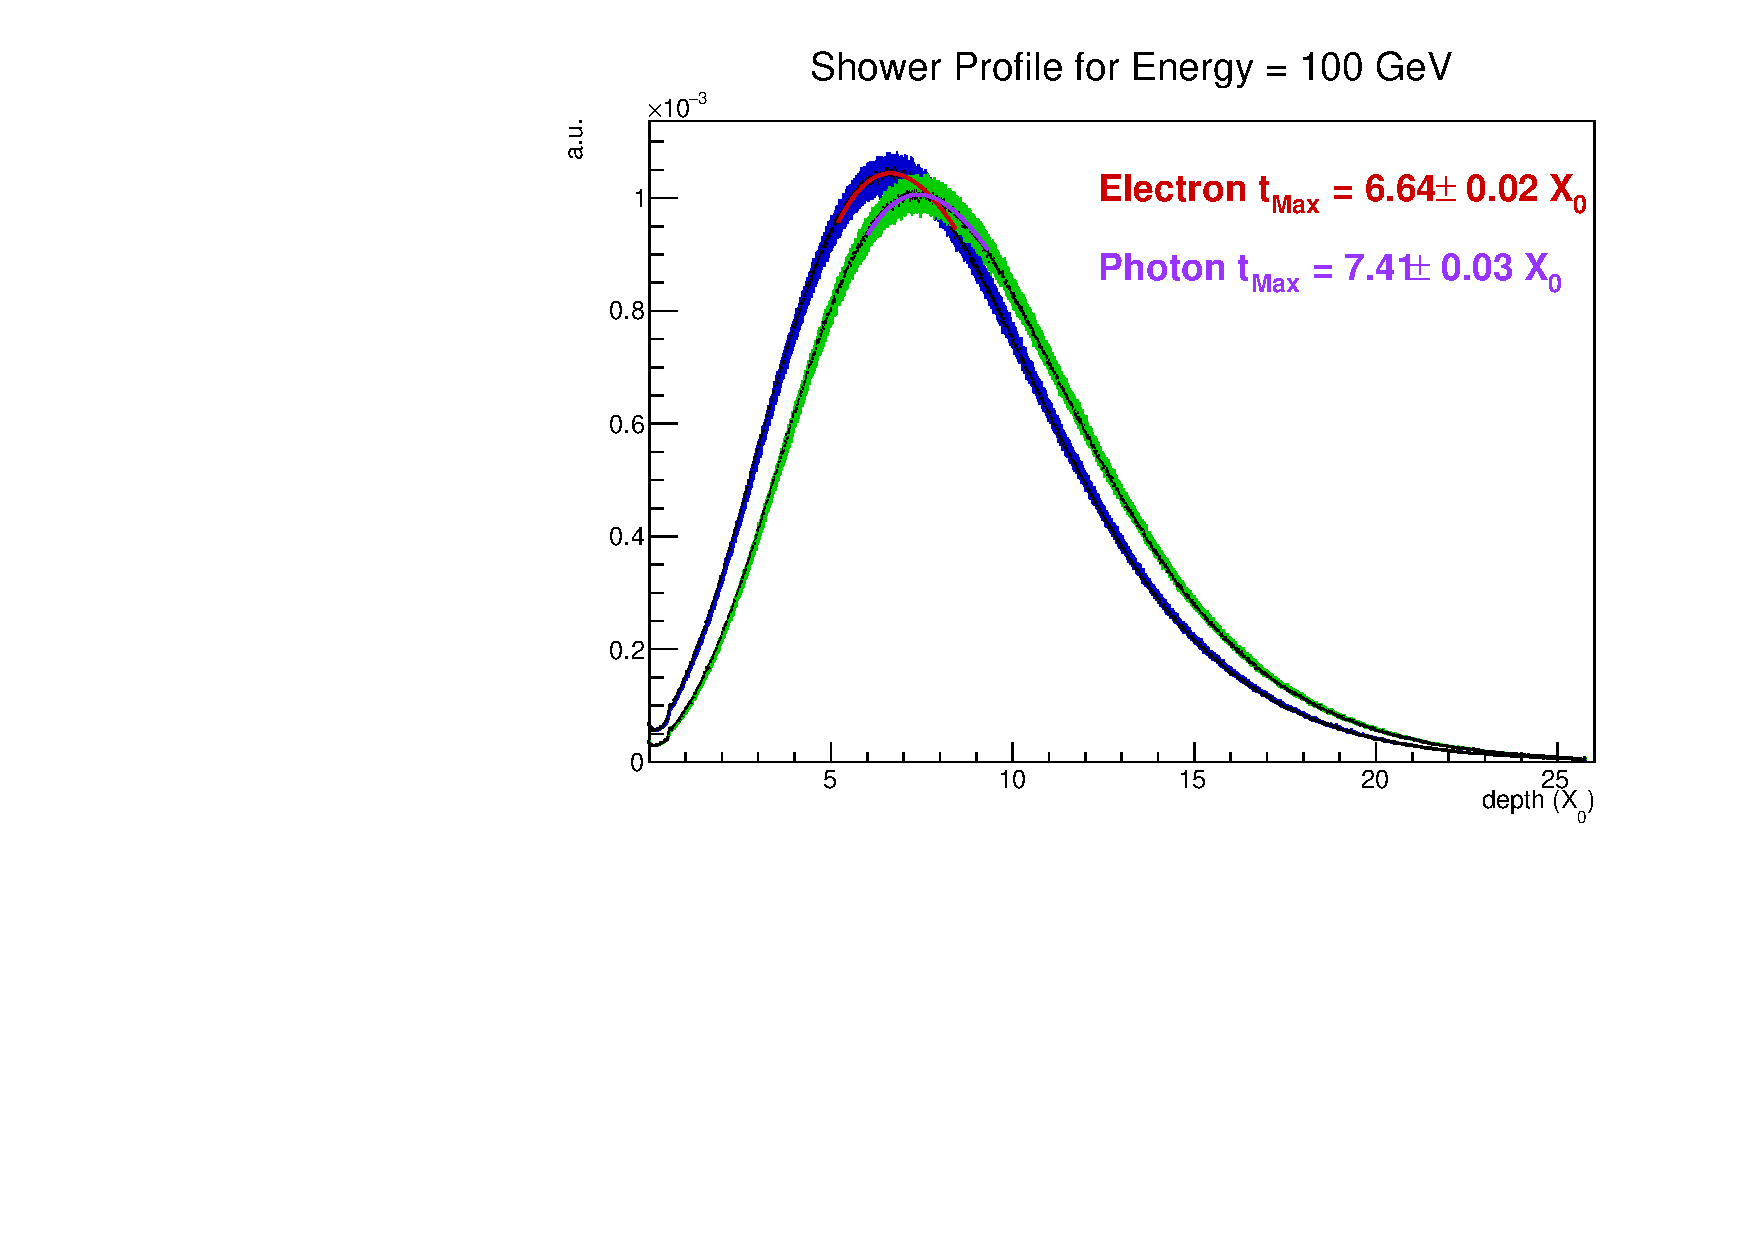
\includegraphics[width=0.55\textwidth]{07-figures/showerProfile_comparison_energy_100_GeV.pdf}
\caption[Longitudinal shower profiles: 100 GeV]{Characteristic shower profiles for 100 GeV electrons and photons in ECAL crystals. The shower maximum is extracted from a fit of a Longo-Sestelli function to the profile.}
\label{fig:shower_profiles}
\end{figure} 

\begin{figure}[hbtp!]
\centering
            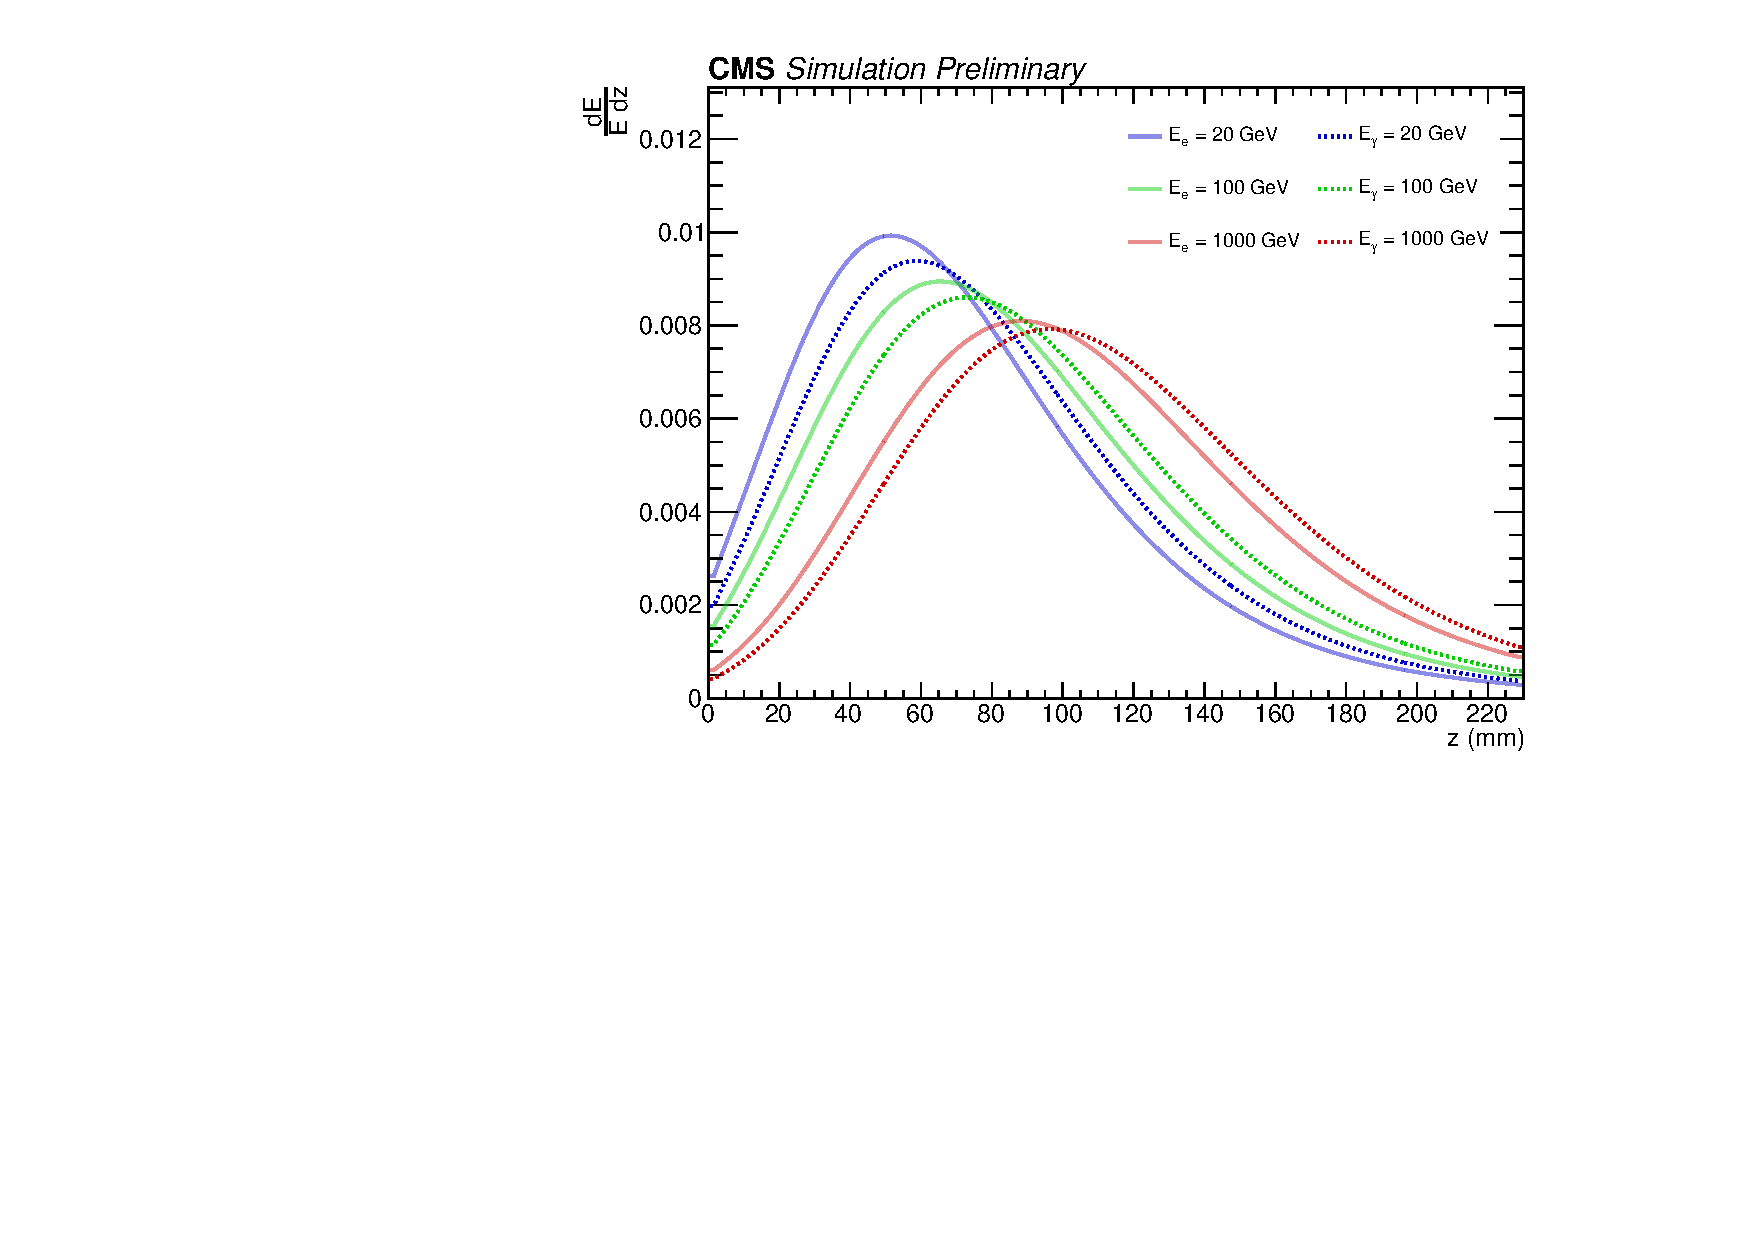
\includegraphics[width=0.75\textwidth]{07-figures/ShowerProfiles_comparison_inEB.pdf}
    \caption[Longitudinal shower profiles: 20, 100, 1000 GeV]{Average depth of the shower maximum in mm for 20 GeV, 100 GeV, and 1000 GeV electrons (solid) and photons (dashed) taken from~\cite{fnuf_dps_note}.}
    \label{fig:shower_profiles_per_energy}
\end{figure}

The transmission of light in ECAL crystals can be approximated by a light attenuation coefficient $\mu$. Initially, when the crystals were first installed, the light attenuation length was small with typical values of $\mu_{\mathrm{nat}}$ = 0.30 $\pm$ 0.01 m$^{-1}$, corresponding to an optical attenuation length of $\sim$3 m in the 22 cm crystals. At that time, the LCE was nearly uniform with slight differences due to the geometry of the crystals. After irradiation the LCE varies as a function of depth, and the loss in transparency due to irradiation is modeled by adding an induced light attenuation coefficient $\mu_{\mathrm{ind}}$ such that the transparency is
\begin{equation}
    T_{\mathrm{final}} = T_0 * e^{-(\mu_{\mathrm{nat}} + \mu_{\mathrm{ind}}}) L
\end{equation}
where $T_{\mathrm{final}}$ and $T_0$ are the final and initial light transmission, and $L$ is the average light path length through the crystal.

Since the radiation dose to the crystals increases with time, and the residual photon energy scale corrections are derived using electrons from Z boson decays, a correction is needed to compensate for the difference in signals from electrons and photons. This correction is called the 'front non-uniformity factor' (FNUF) since the non-uniformity is largest around the shower maximum for electrons, near the front face of the crystal. It is applied to photon energies as:

\begin{equation}
    F = \frac{S_{\gamma}}{S_e} = \frac{\frac{\int E^{\gamma}_{dep}(z) * LCE(z) dz}{\int E^{\gamma}_{dep}(z) dz}}{\frac{\int E^{e}_{dep}(z) * LCE(z) dz}{\int E^{e}_{dep}(z) dz}},
    \label{eqn:fnuf}
\end{equation}

\noindent where $E^{e}_{dep}(z)$ and $E^{\gamma}_{dep}(z)$ are the energy deposition profiles for electrons and photons of the same energy. 

The dependence of the LCE on radiation damage is estimated with the ECAL Longevity Model (ELM)~\cite{FNUF1}. This model uses a uniform instantaneous luminosity and a FLUKA~\cite{FLUKA} simulation to estimate the fluxes of hadrons, electrons, and photons. Values of $\mu_{\mathrm{ind}}$ are estimated across the entire ECAL (0 $< |\eta| <$ 3 in steps of 0.1) for different values of integrated luminosity. Each scenario is simulated using the S-Litrani~\cite{Gentit200235} light simulation and accounts for the loss of gain and sensitivity in the photodetectors. 

The ELM derives LCE models in bins of |$\eta$| and integrated luminosity, and from the integrated luminosity it derives values of R/R$_0$. Hence, by knowing the value of R/R$_0$ in data, an LCE model can be selected for every event. The measured values of R/R$_0$ in the EB and EE, shown in Figures~\ref{fig:rr0_vs_run_EB} and ~\ref{fig:rr0_vs_run_EE} taken from~\cite{CMS-DP-2019-005}, are used to select corresponding LCE functions, which are shown in Figure~\ref{fig:lce_profiles}~\cite{fnuf_dps_note}.  FNUF corrections, as a function of energy, |$\eta$|, and R/R$_0$ are computed using photon and electron showers simulated at several energies and weighted with the LCE functions, as shown in Equation~\ref{eqn:fnuf}. These corrections are shown in Figure~\ref{fig:fnuf_vs_energy}~\cite{fnuf_dps_note}. Note again that this correction is only relevant to photons whose shower maximum significantly differs from that of electrons. The shower maximum of low R$_9$ (R$_9 < 0.96$) photons, having likely converted to an electron-positron pair before the ECAL, is nearly identical to low R$_9$ electrons. The shower maxima for low R$_9$ photons and electrons are shown in Figure~\ref{fig:lowR9_shower_max}. The similarity of the location of the shower maxima means that no FNUF correction is needed for these photons, and no correction is made.

\begin{figure}[htbp!]
    \subfloat{%
        \begin{minipage}[t]{0.5\textwidth}%
            \begin{center}
                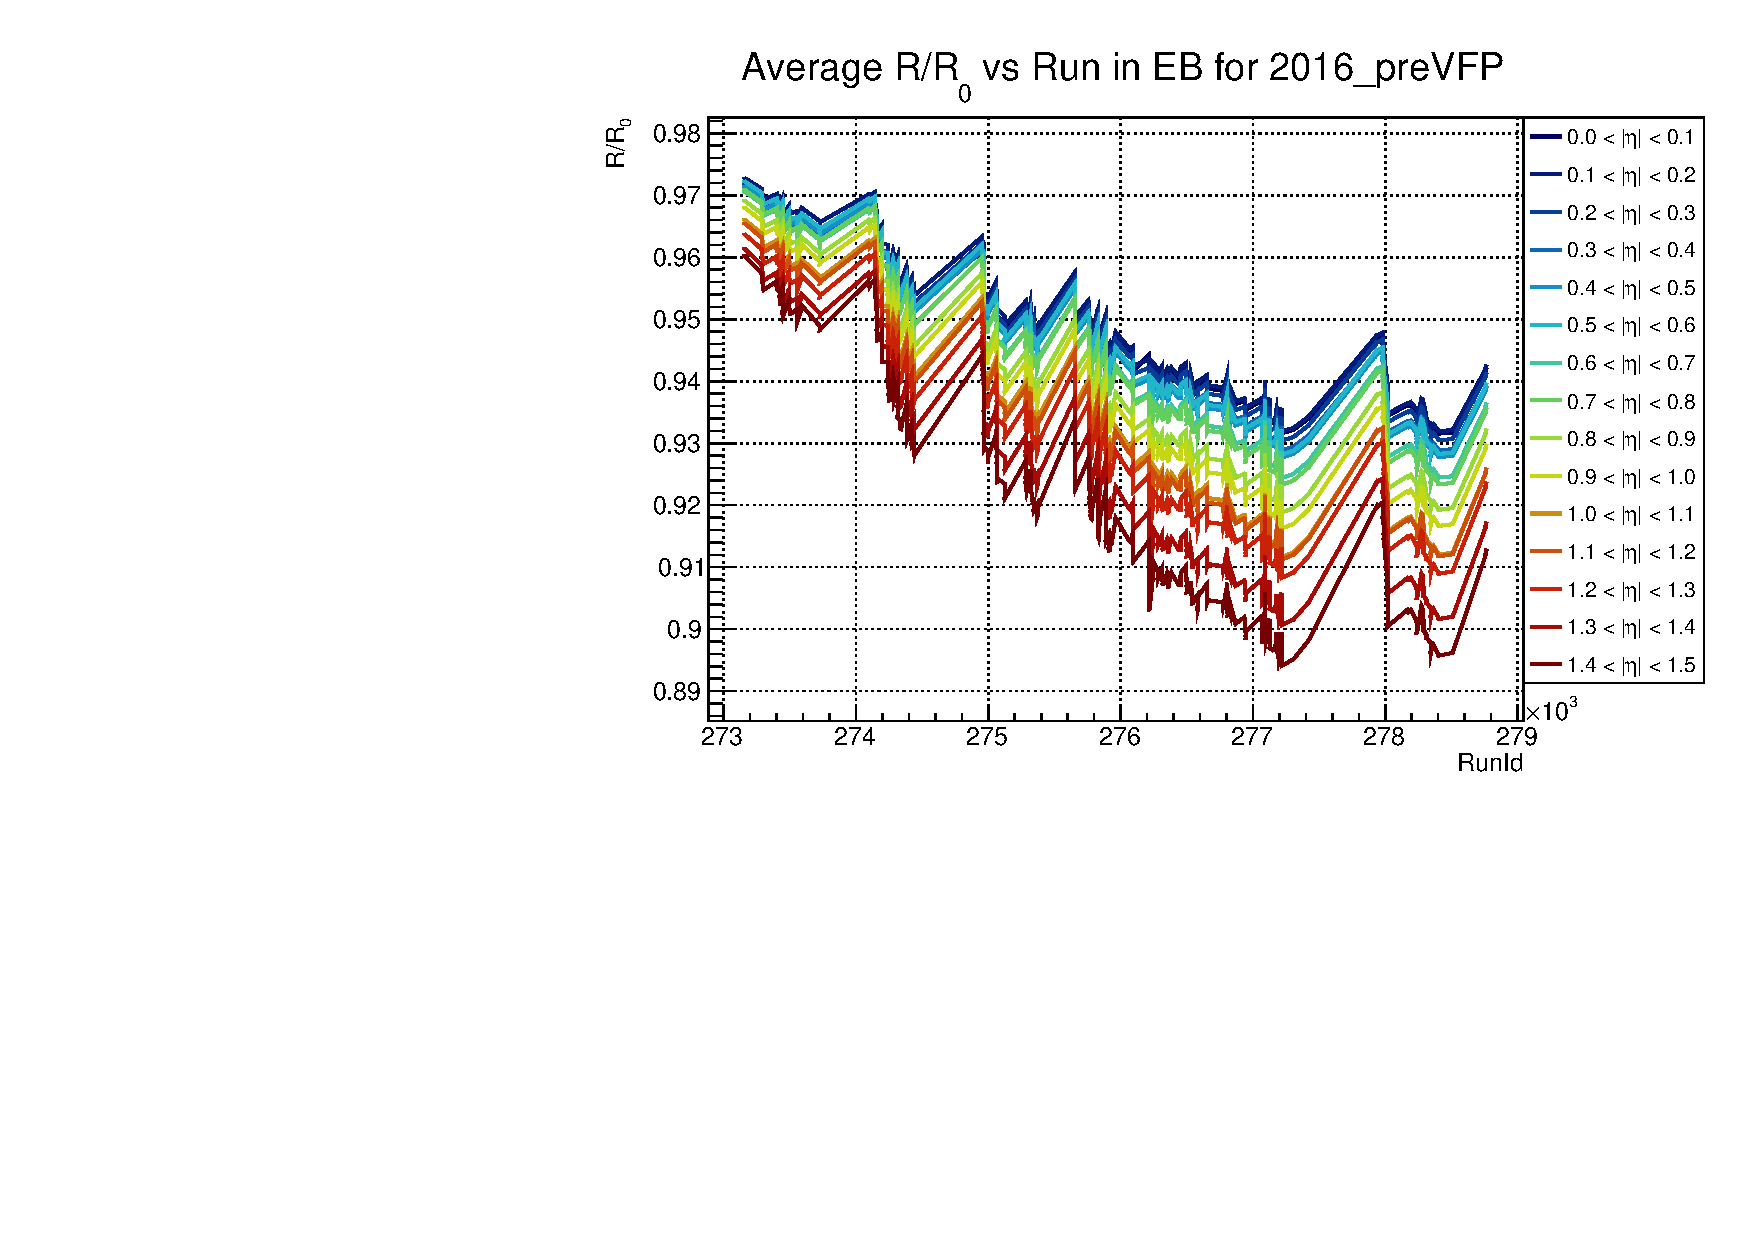
\includegraphics[width=\textwidth]{07-figures/average_RoverR0_2016_preVFP_inEB.pdf}
            \end{center}
        \end{minipage}
    }
    \subfloat{
        \begin{minipage}[t]{0.5\textwidth}%
            \begin{center}
                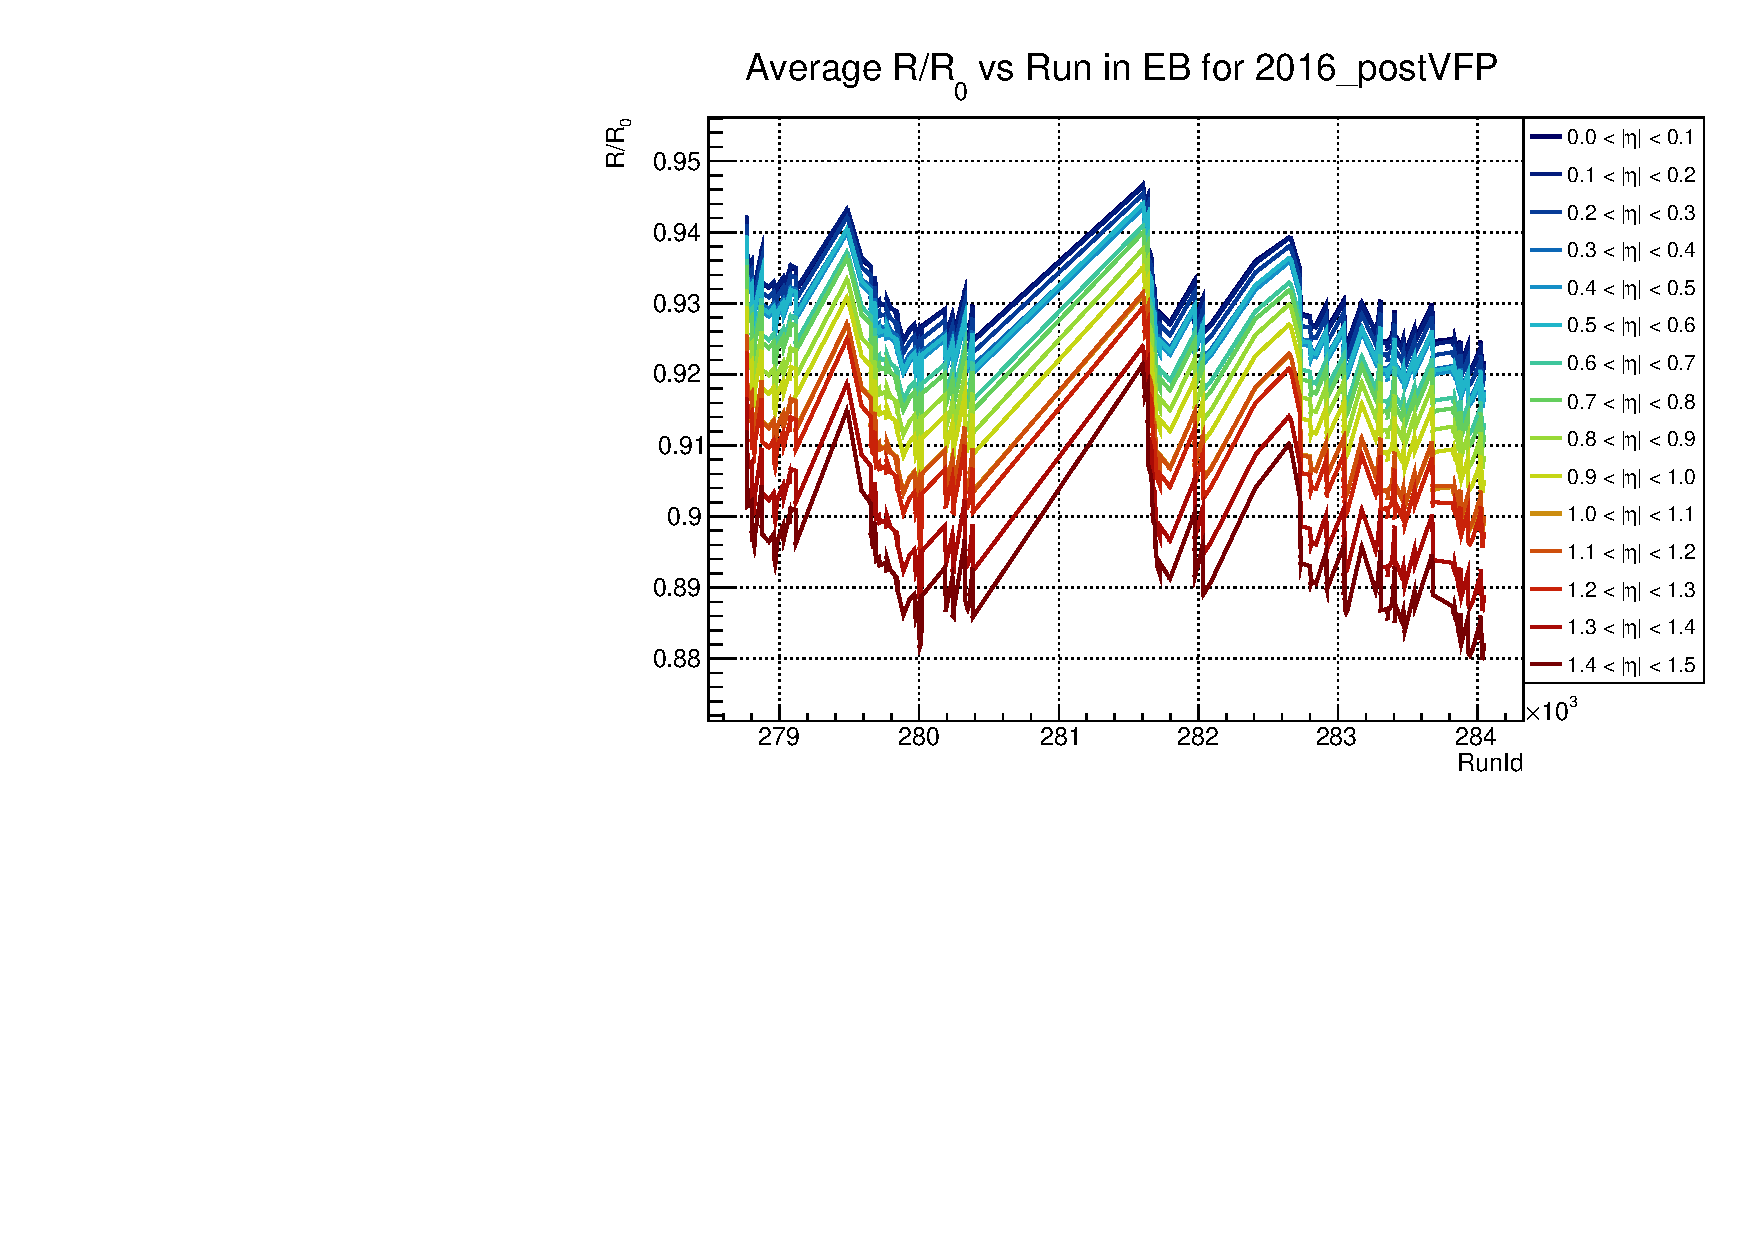
\includegraphics[width=\textwidth]{07-figures/average_RoverR0_2016_postVFP_inEB.pdf}
            \end{center}
        \end{minipage}
    }~\subfloat{
        \begin{minipage}[t]{0.5\textwidth}%
            \begin{center}
                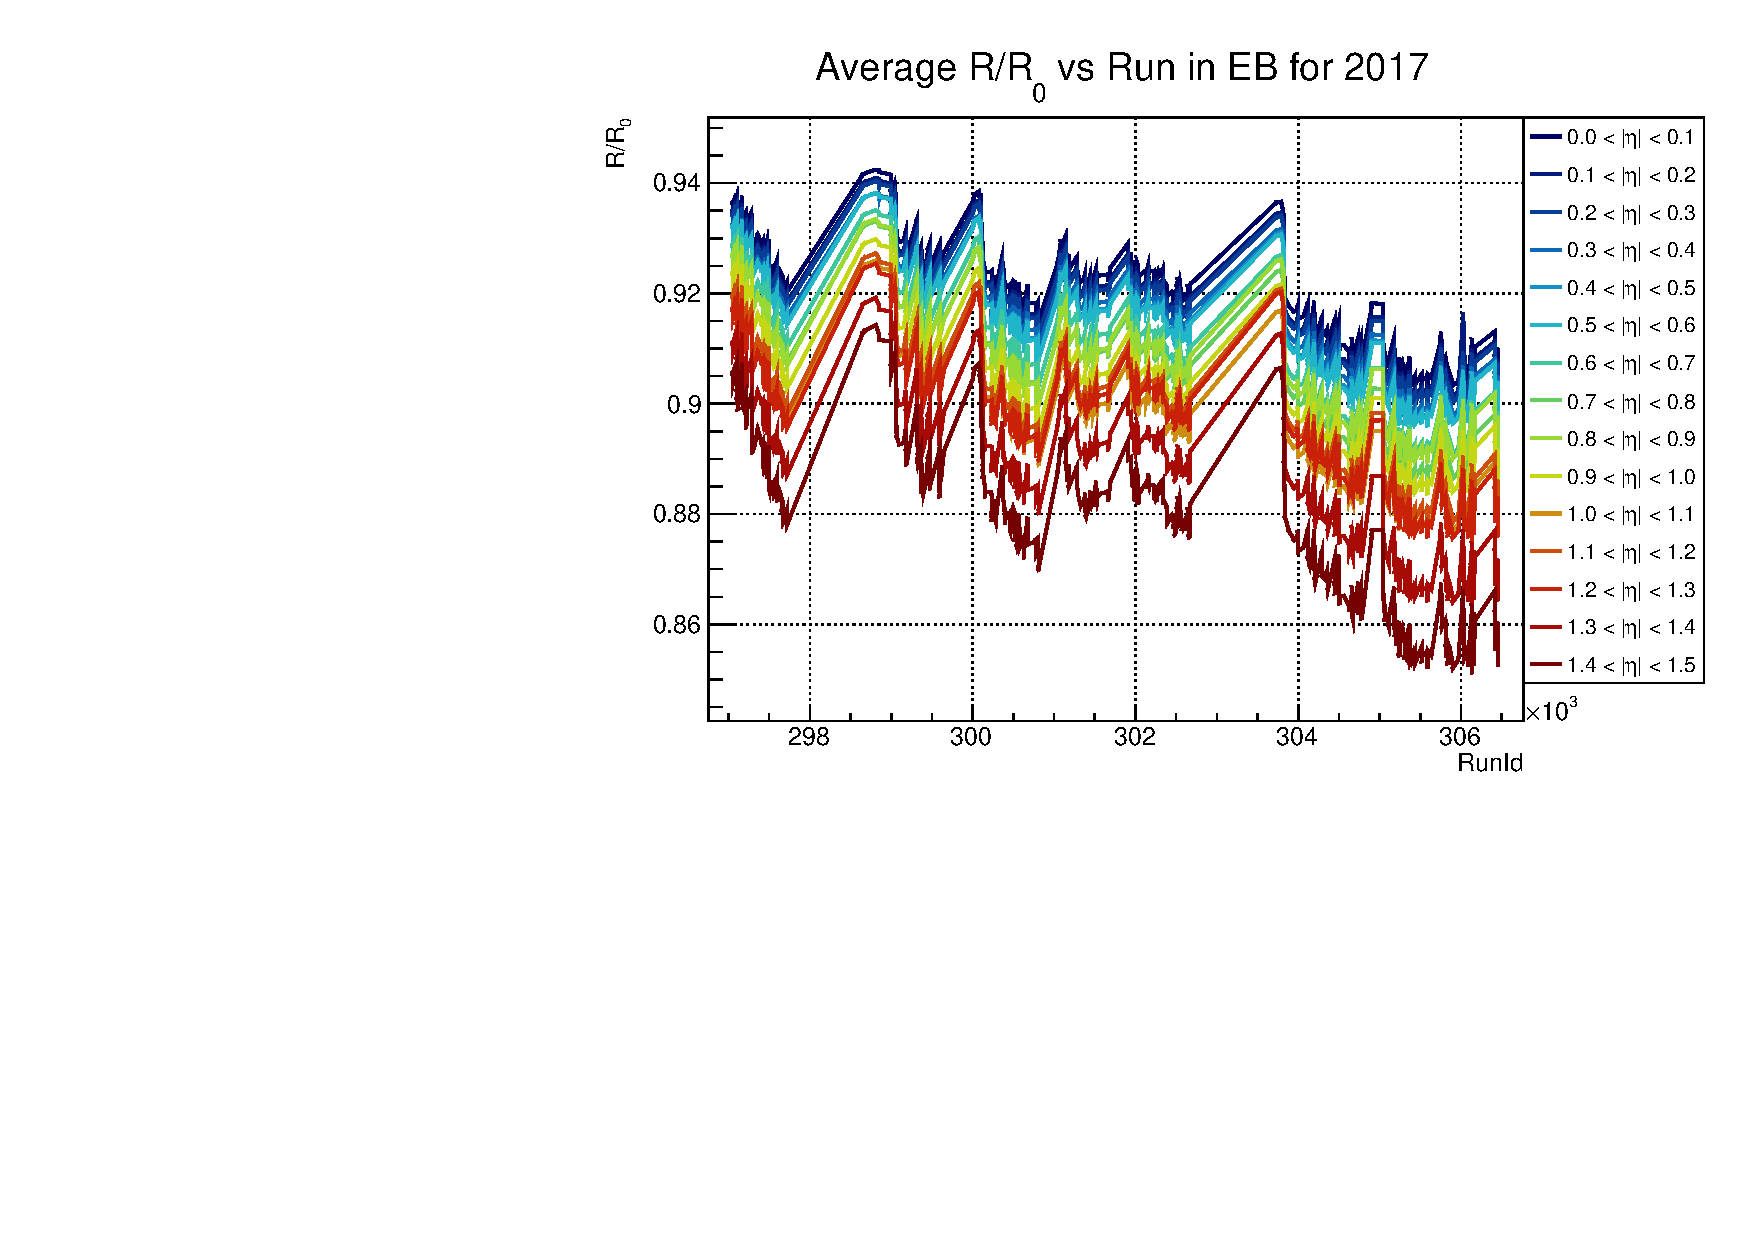
\includegraphics[width=\textwidth]{07-figures/average_RoverR0_2017_inEB.pdf}
            \end{center}
        \end{minipage}
    }~\subfloat{
        \begin{minipage}[t]{0.5\textwidth}%
            \begin{center}
                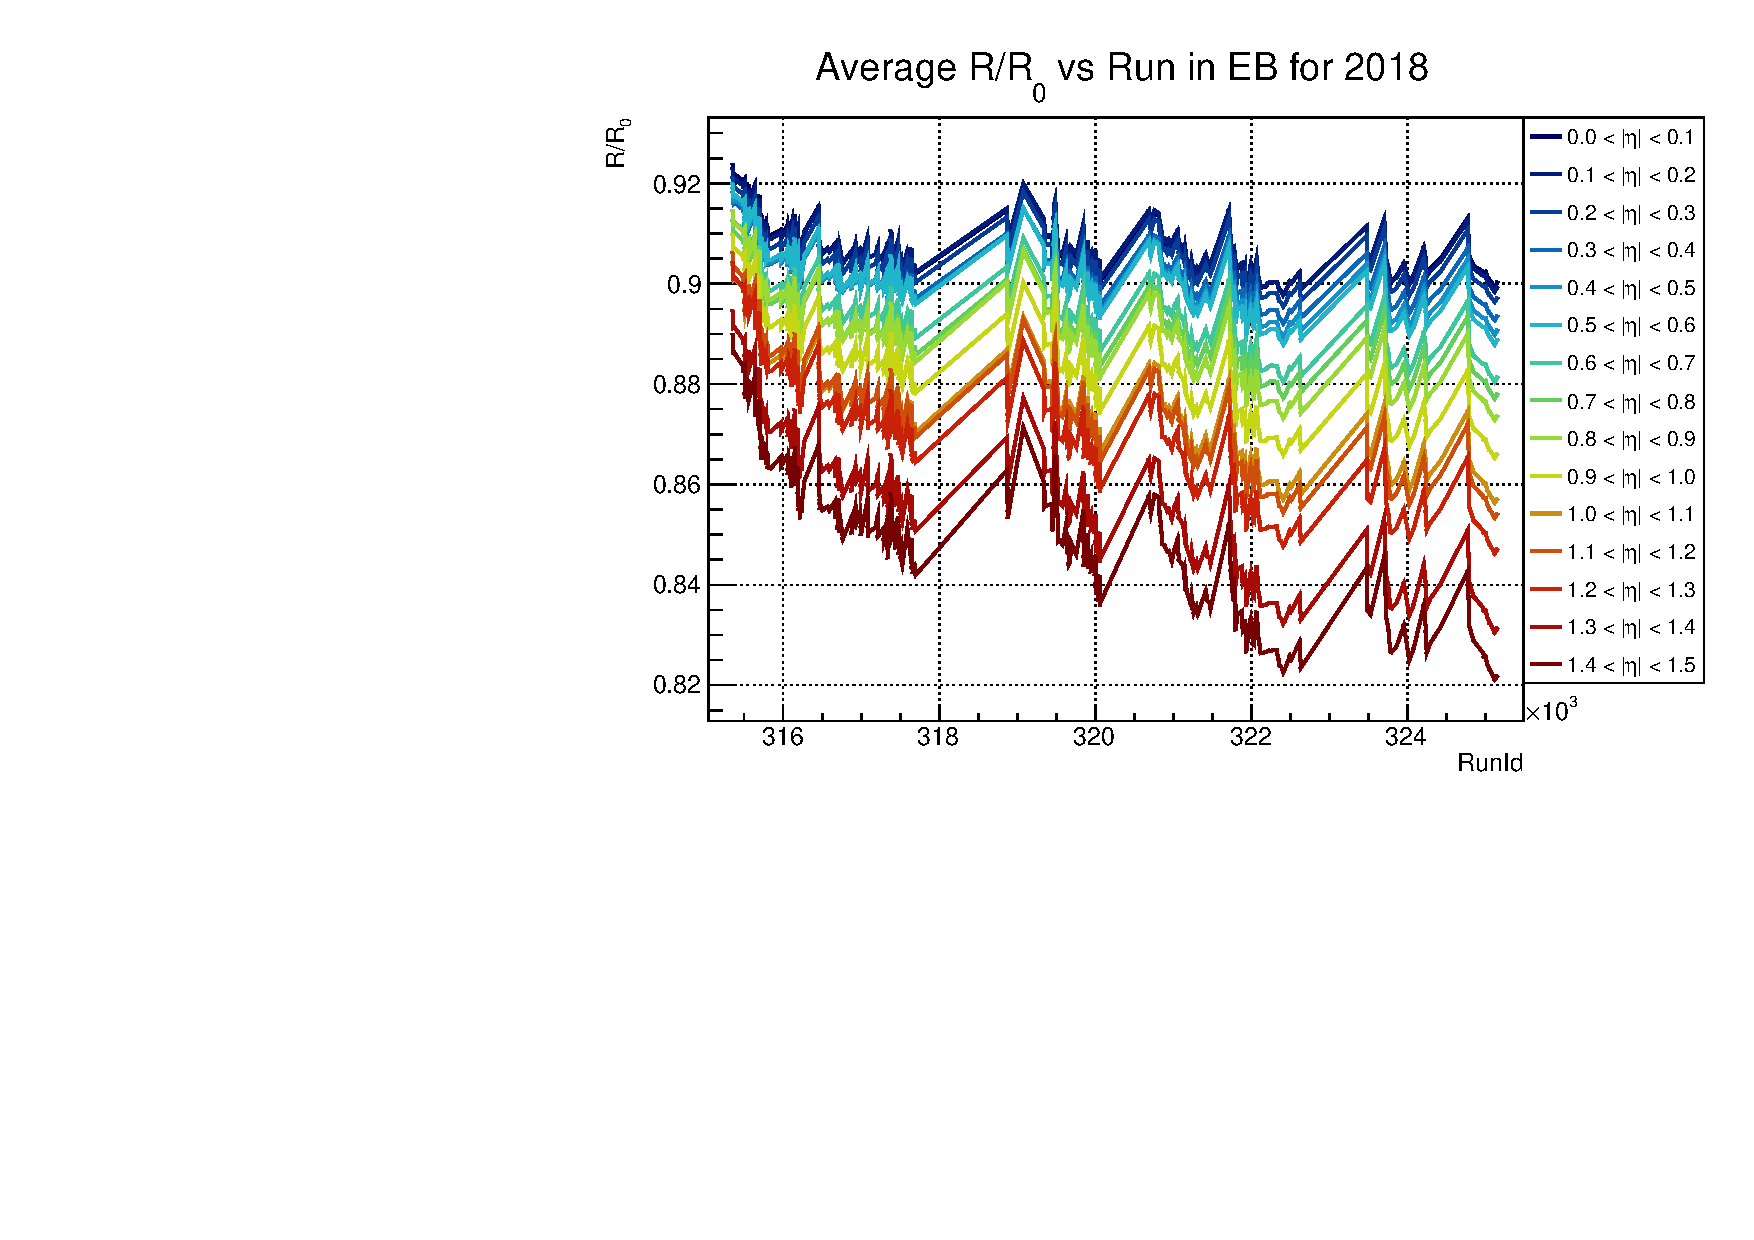
\includegraphics[width=\textwidth]{07-figures/average_RoverR0_2018_inEB.pdf}
            \end{center}
        \end{minipage}
    }
    \caption[Average laser response: EB]{Average R/R$_{0}$ from laser measurements as a function of the run, for different $|\eta|$-bins in EB taken from~\cite{CMS-DP-2019-005}.}
    \label{fig:rr0_vs_run_EB}
\end{figure}

\begin{figure}[htbp!]
    \subfloat{%
        \begin{minipage}[t]{0.5\textwidth}%
            \begin{center}
                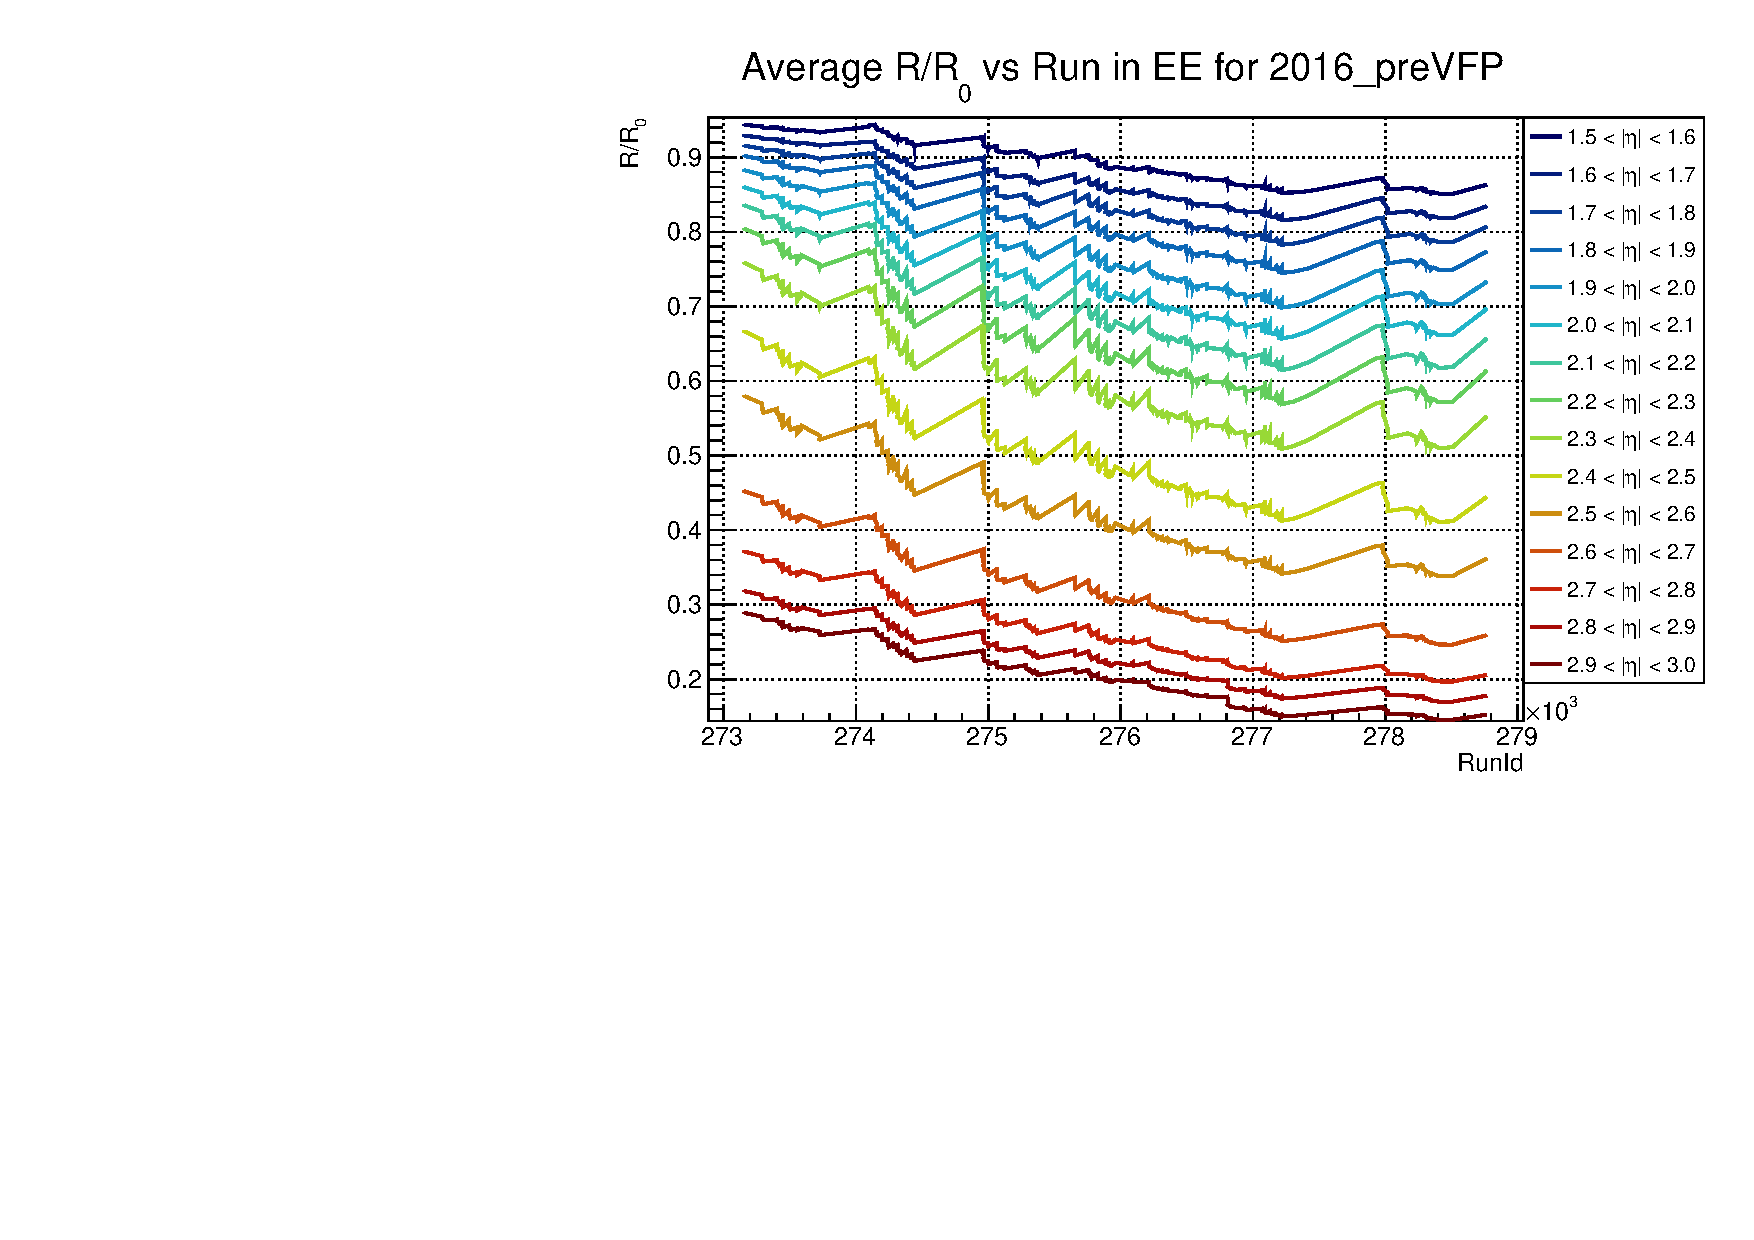
\includegraphics[width=\textwidth]{07-figures/average_RoverR0_2016_preVFP_inEE.pdf}
            \end{center}
        \end{minipage}
    }~\subfloat{%
        \begin{minipage}[t]{0.5\textwidth}%
            \begin{center}
                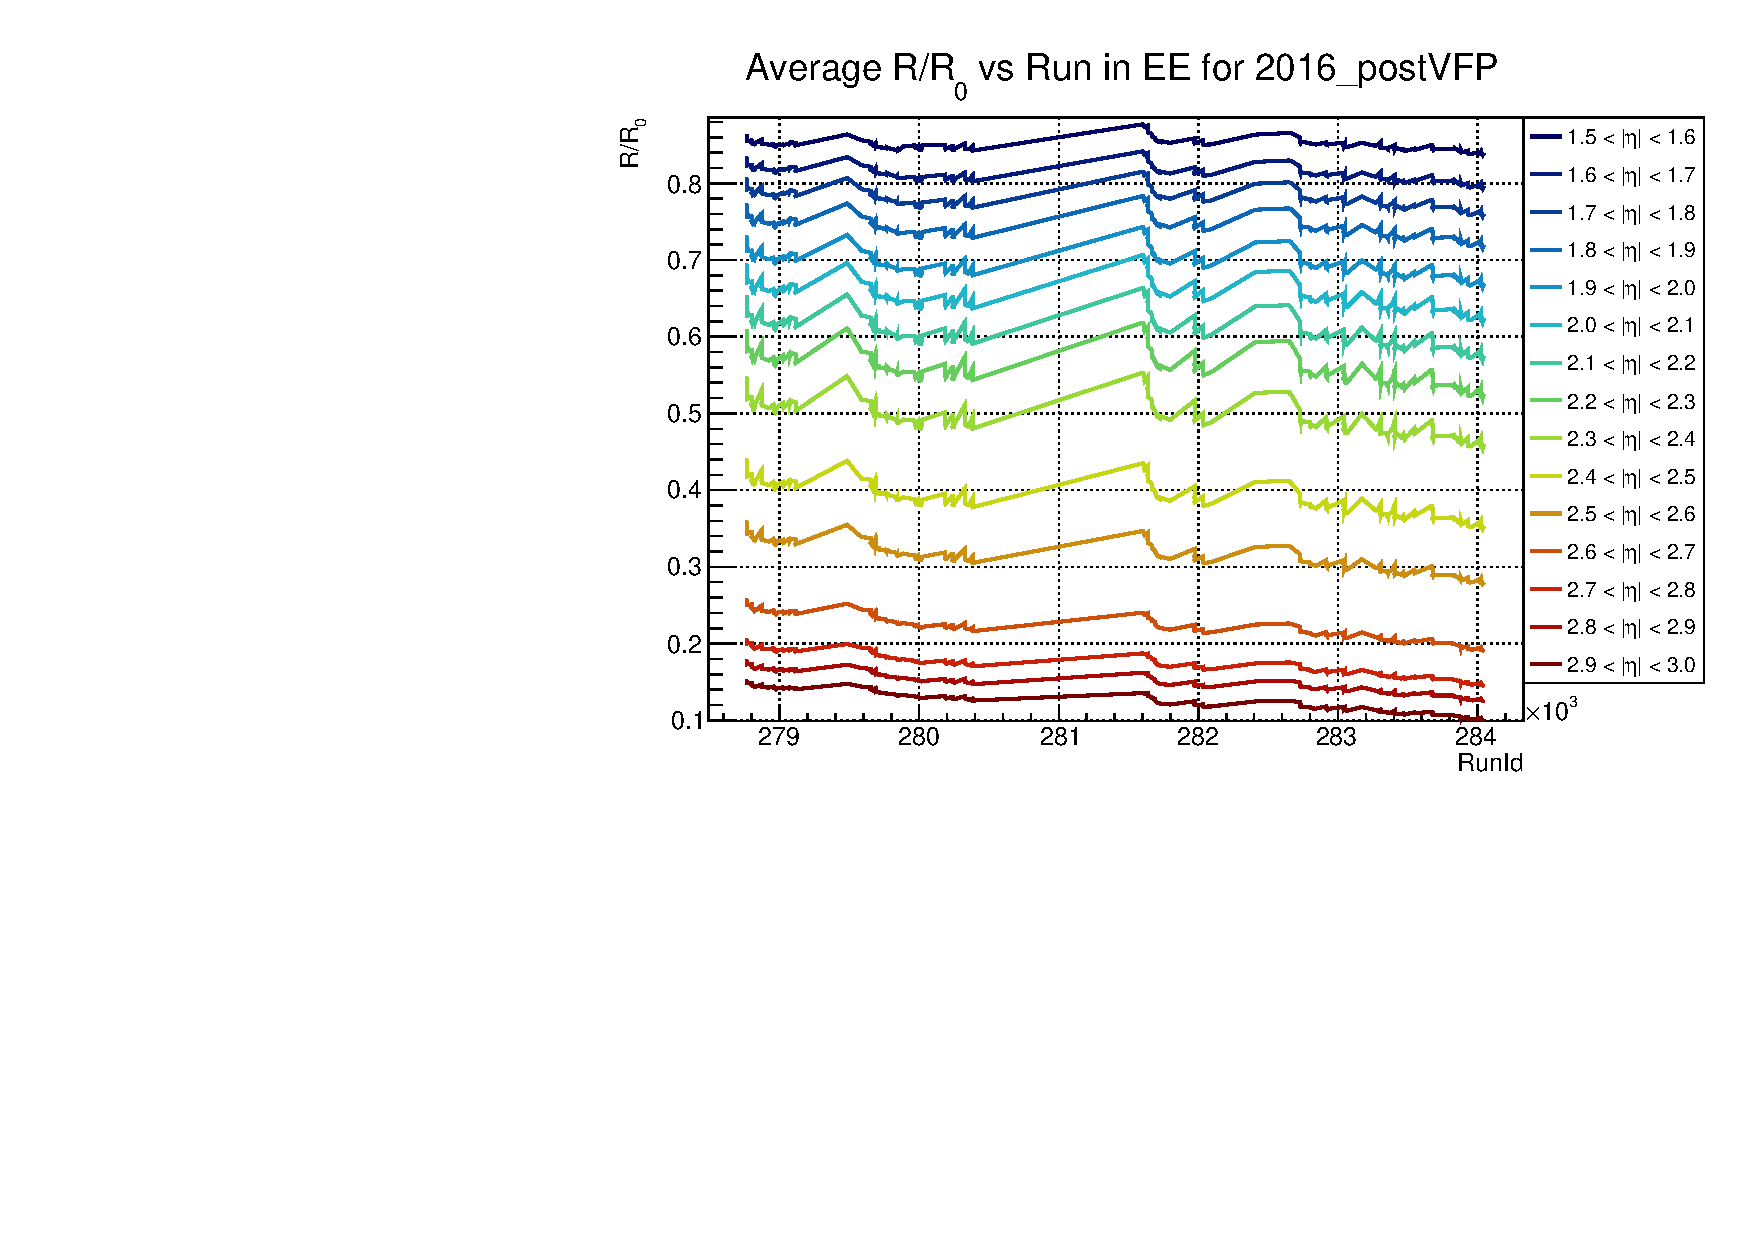
\includegraphics[width=\textwidth]{07-figures/average_RoverR0_2016_postVFP_inEE.pdf}
            \end{center}
        \end{minipage}
    }~\subfloat{%
        \begin{minipage}[t]{0.5\textwidth}%
            \begin{center}
                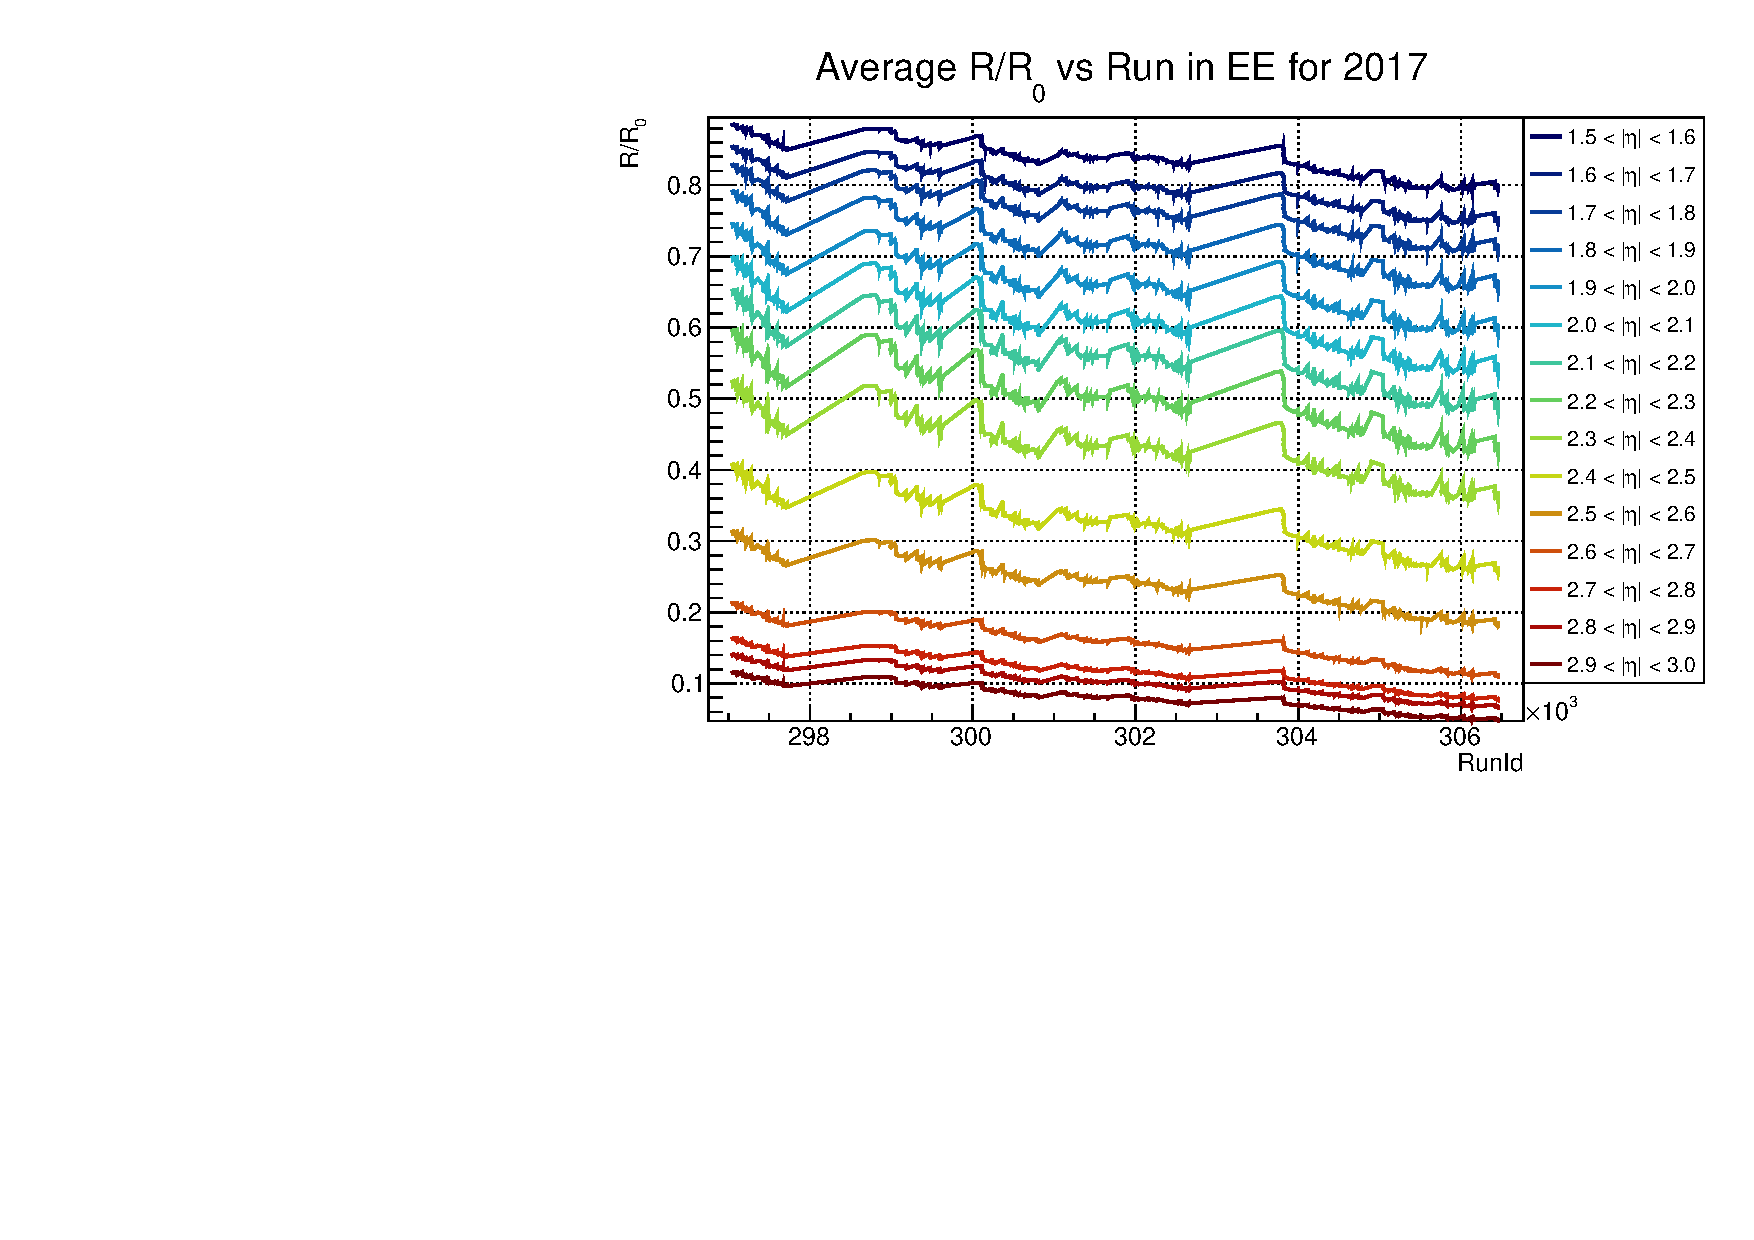
\includegraphics[width=\textwidth]{07-figures/average_RoverR0_2017_inEE.pdf}
            \end{center}
        \end{minipage}
    }~\subfloat{%
        \begin{minipage}[t]{0.5\textwidth}%
            \begin{center}
                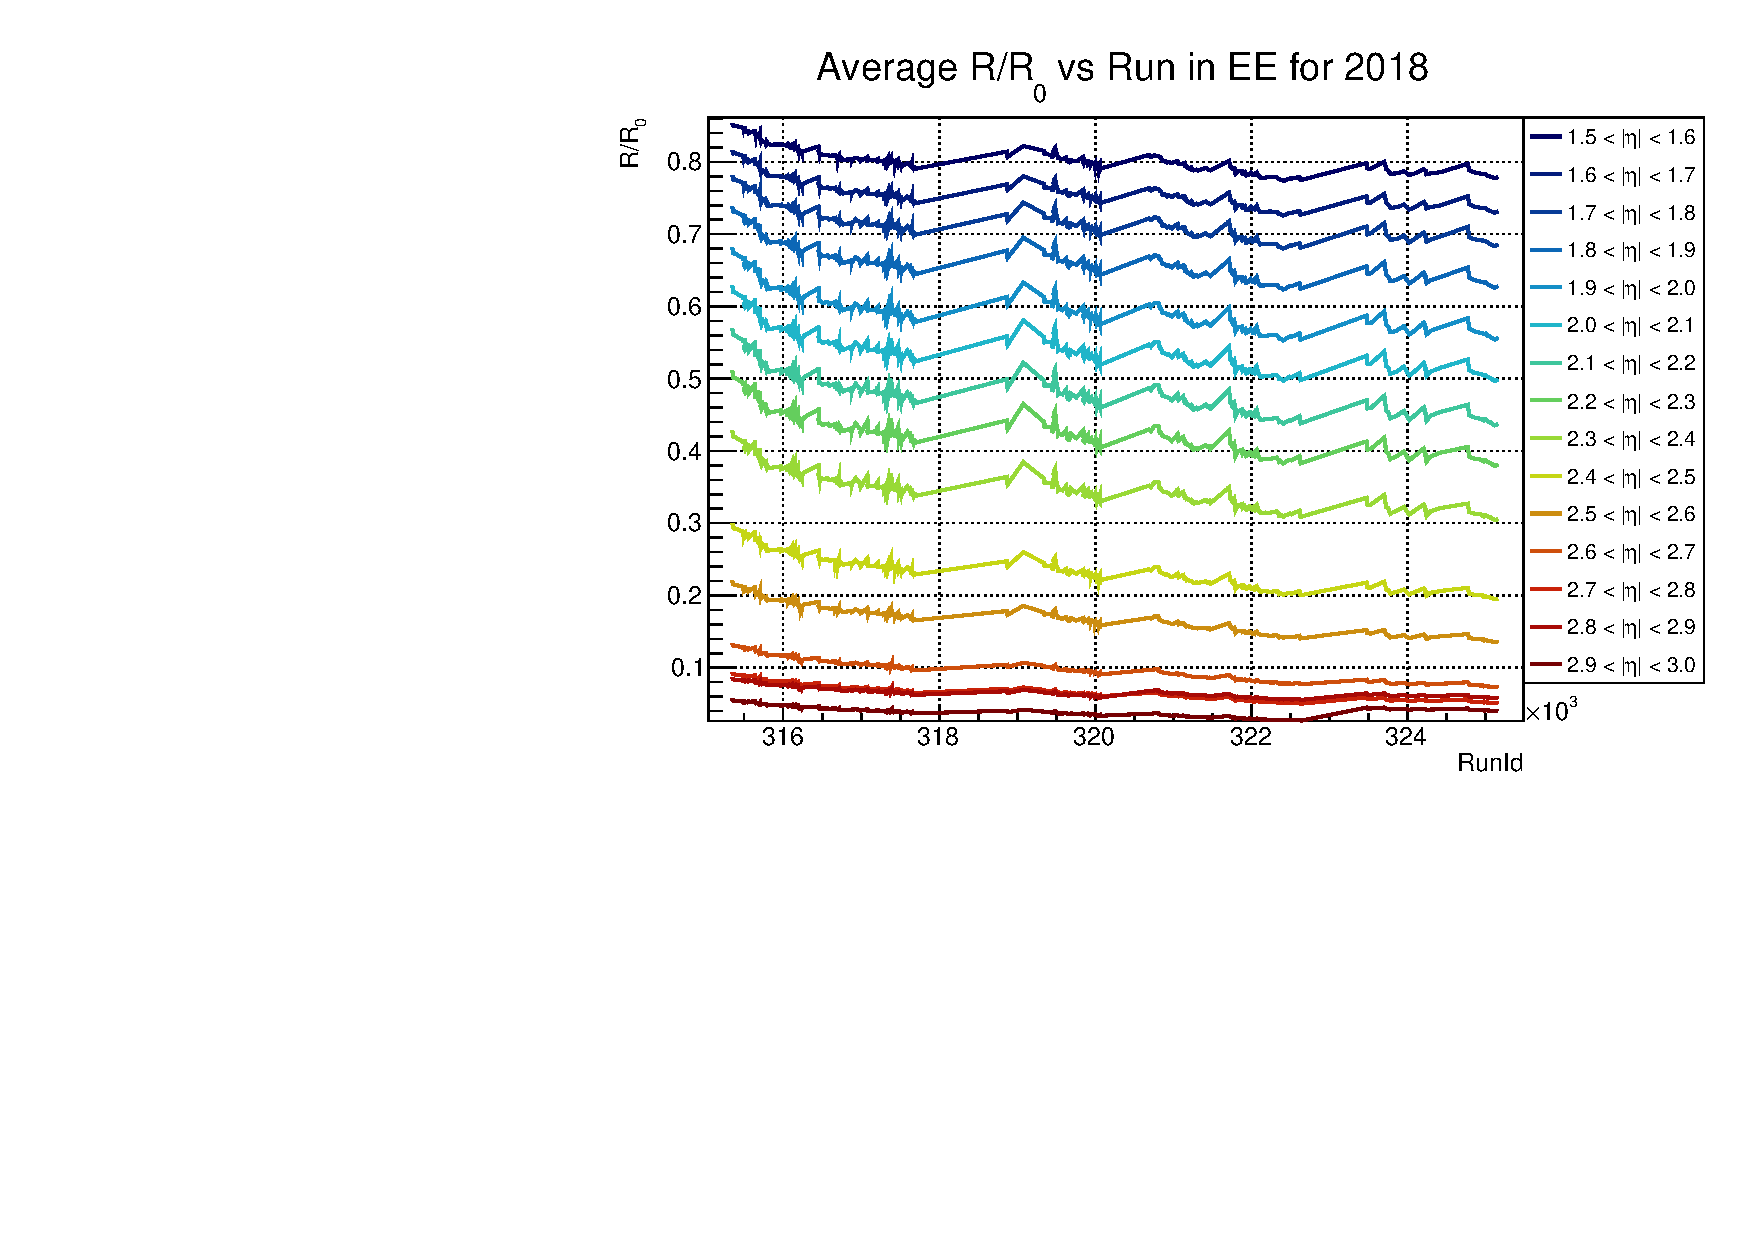
\includegraphics[width=\textwidth]{07-figures/average_RoverR0_2018_inEE.pdf}
            \end{center}
        \end{minipage}
    }
    \caption[Average laser response: EE]{Average R/R$_{0}$ from laser measurements as a function of the run, for different $|\eta|$ bins in EE taken from~\cite{CMS-DP-2019-005}.}
    \label{fig:rr0_vs_run_EE}
\end{figure}

\begin{figure}[htbp!]
    \subfloat{%
        \begin{minipage}[t]{0.5\textwidth}%
            \begin{center}
                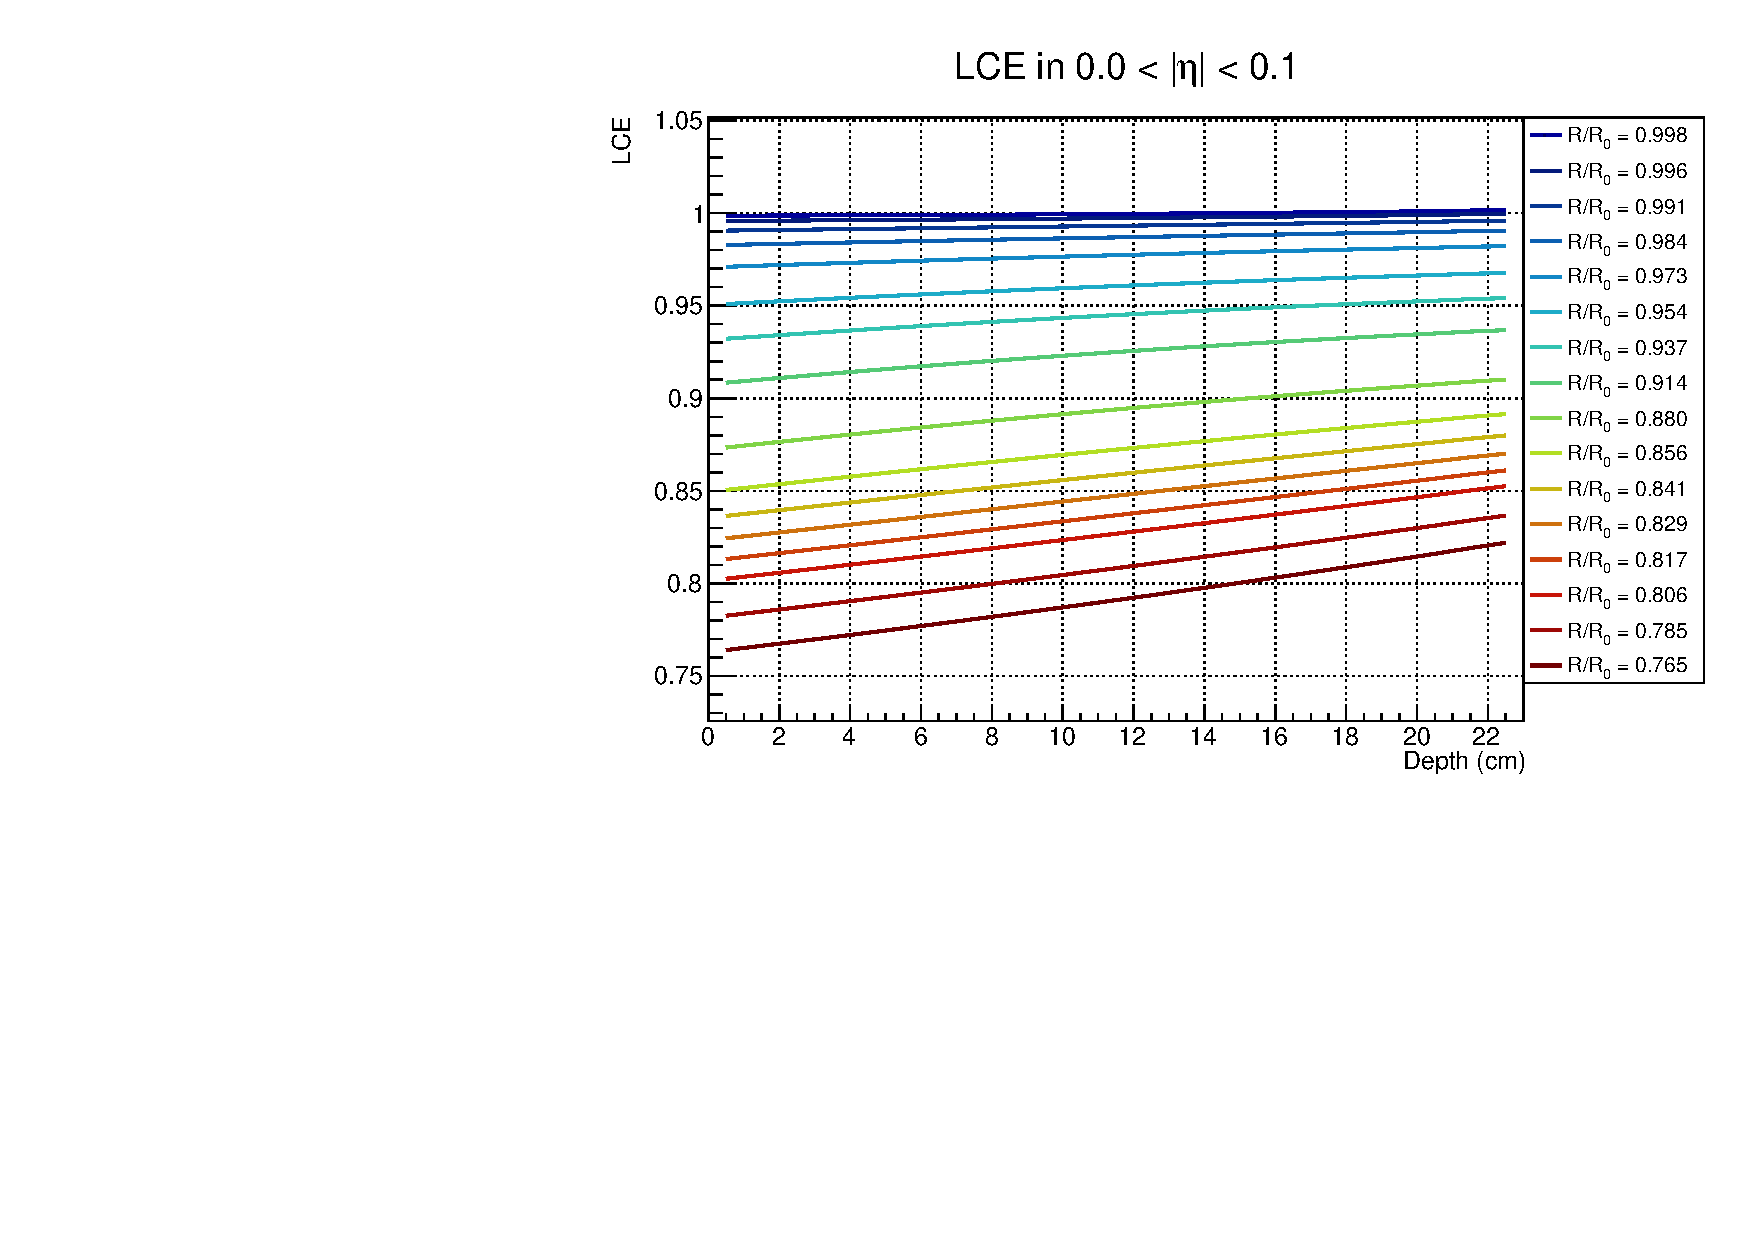
\includegraphics[width=\textwidth]{07-figures/LCE_ring_0_inEB.pdf}
            \end{center}
        \end{minipage}
    }~\subfloat{%
        \begin{minipage}[t]{0.5\textwidth}%
            \begin{center}
                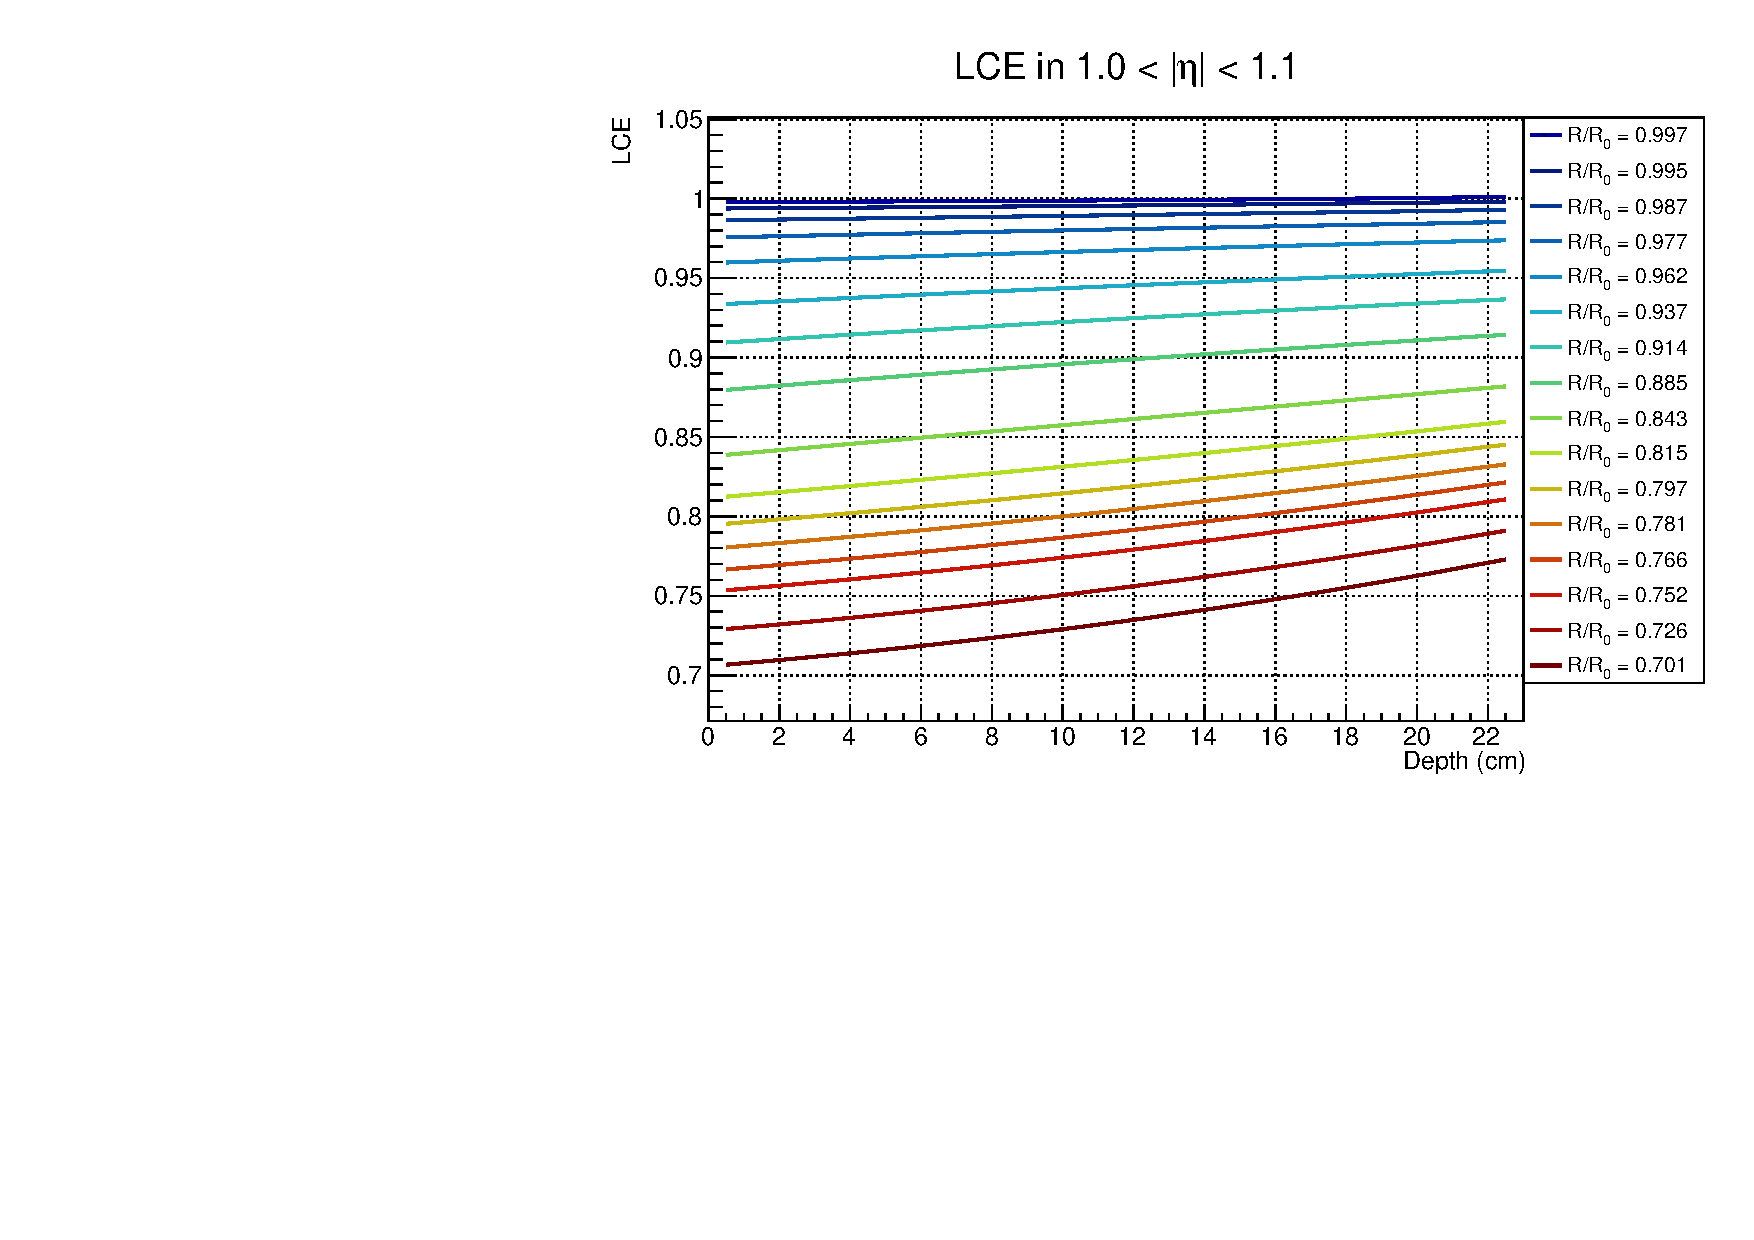
\includegraphics[width=\textwidth]{07-figures/LCE_ring_10_inEB.pdf}
            \end{center}
        \end{minipage}
    }~\subfloat{%
        \begin{minipage}[t]{0.5\textwidth}%
            \begin{center}
                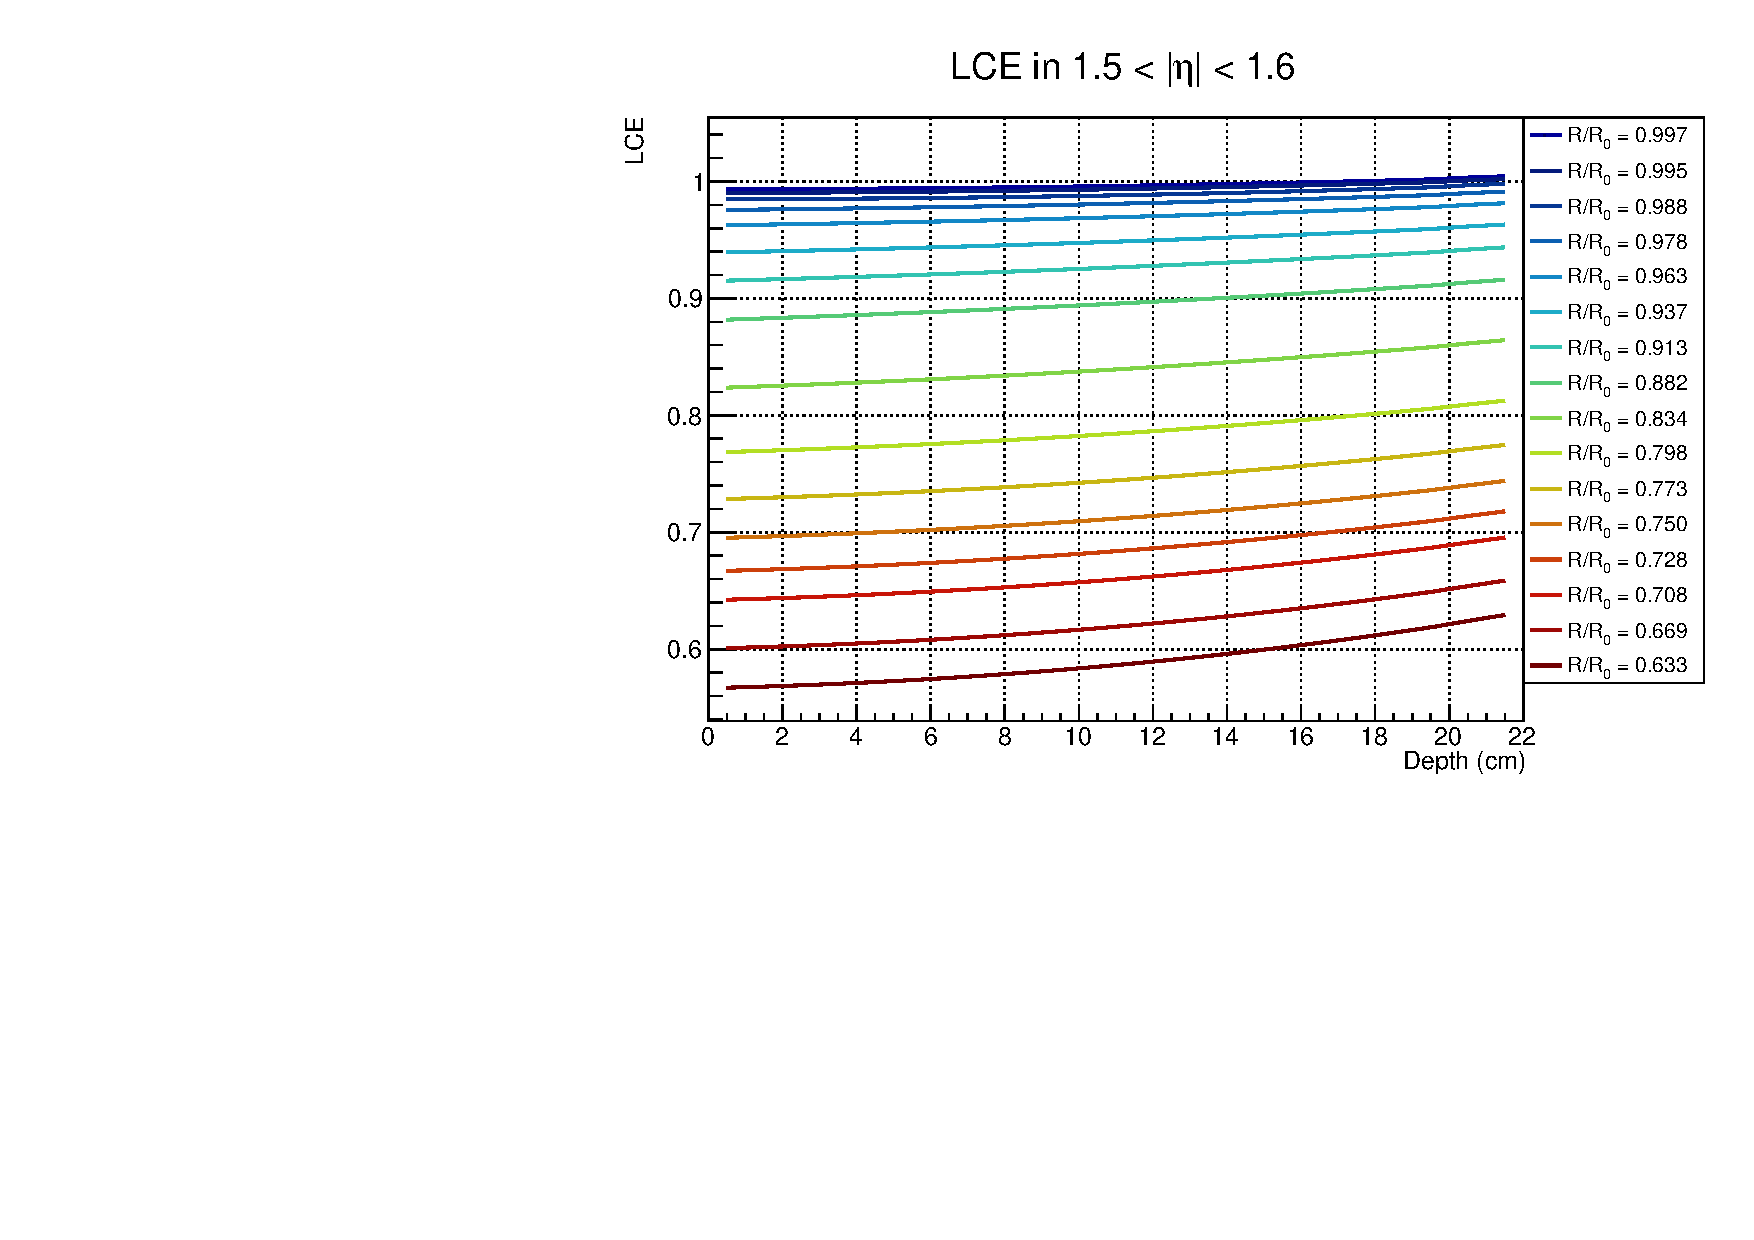
\includegraphics[width=\textwidth]{07-figures/LCE_ring_15_inEE.pdf}
            \end{center}
        \end{minipage}
    }~\subfloat{%
        \begin{minipage}[t]{0.5\textwidth}%
            \begin{center}
                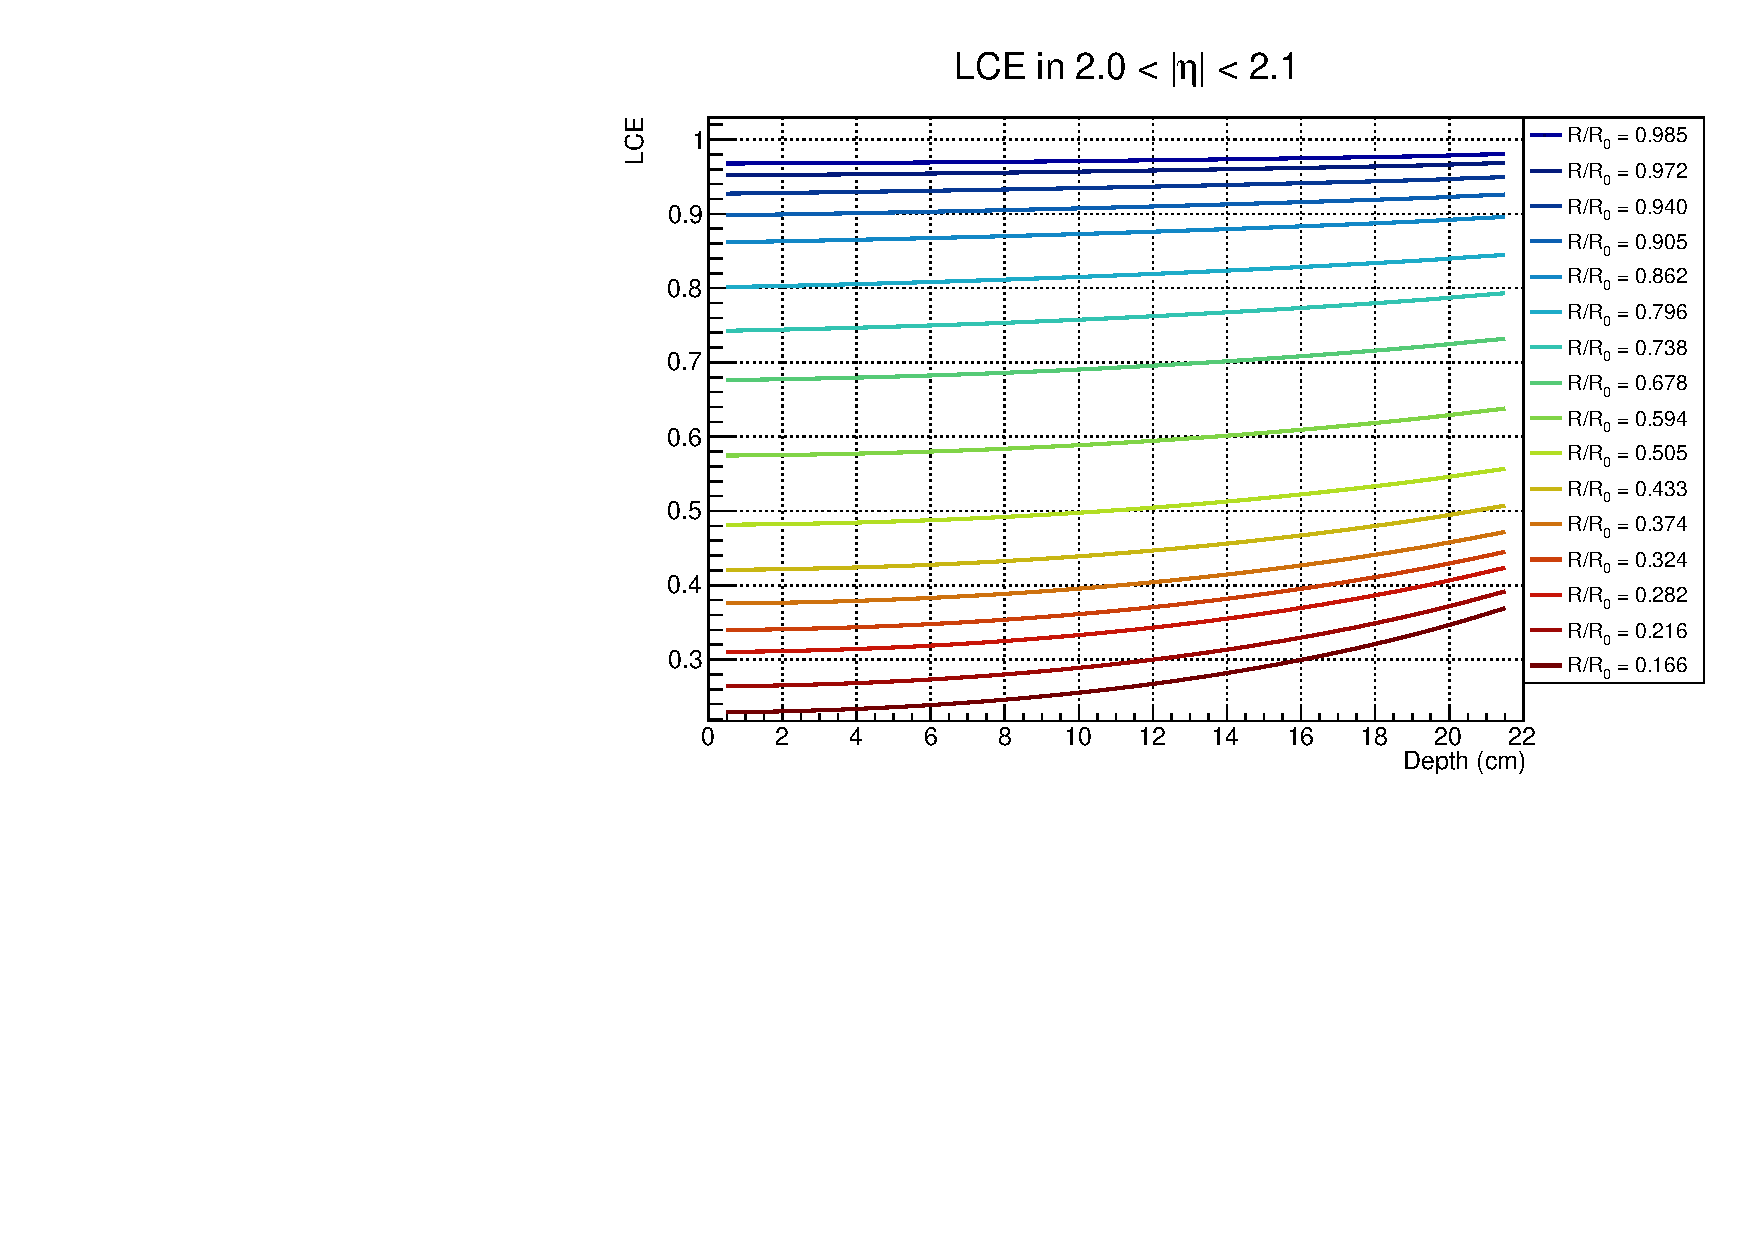
\includegraphics[width=\textwidth]{07-figures/LCE_ring_20_inEE.pdf}
            \end{center}
        \end{minipage}
    }
\caption[Light collection efficiency profiles]{LCE profiles for different value of |$\eta$| in the EB and EE taken from~\cite{fnuf_dps_note}.}
\label{fig:lce_profiles}
\end{figure}

\begin{figure}[htbp!]
    \subfloat{%
        \begin{minipage}[t]{0.5\textwidth}%
            \begin{center}
                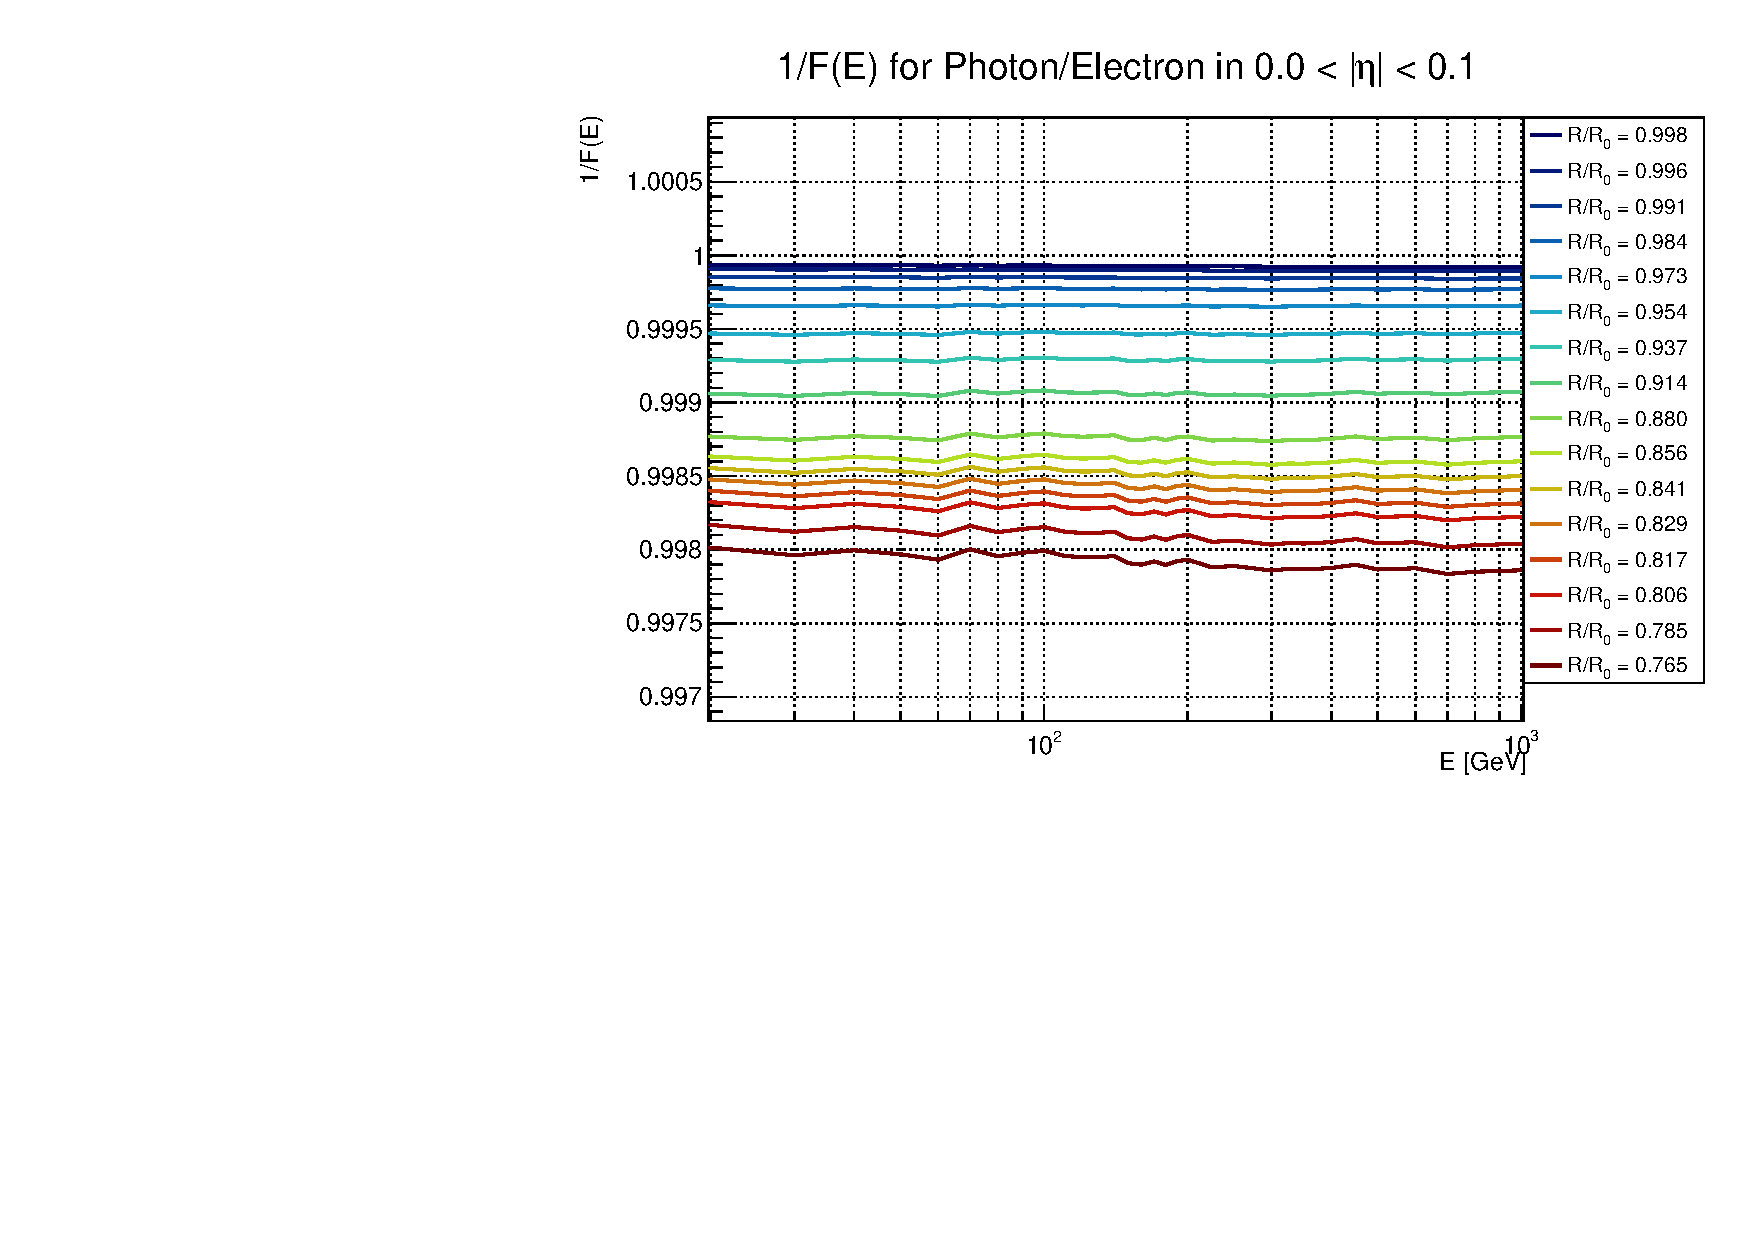
\includegraphics[width=\textwidth]{07-figures/F_vs_E_ratio_ring_0_inEB.pdf}
            \end{center}
        \end{minipage}
    }~\subfloat{%
        \begin{minipage}[t]{0.5\textwidth}%
            \begin{center}
                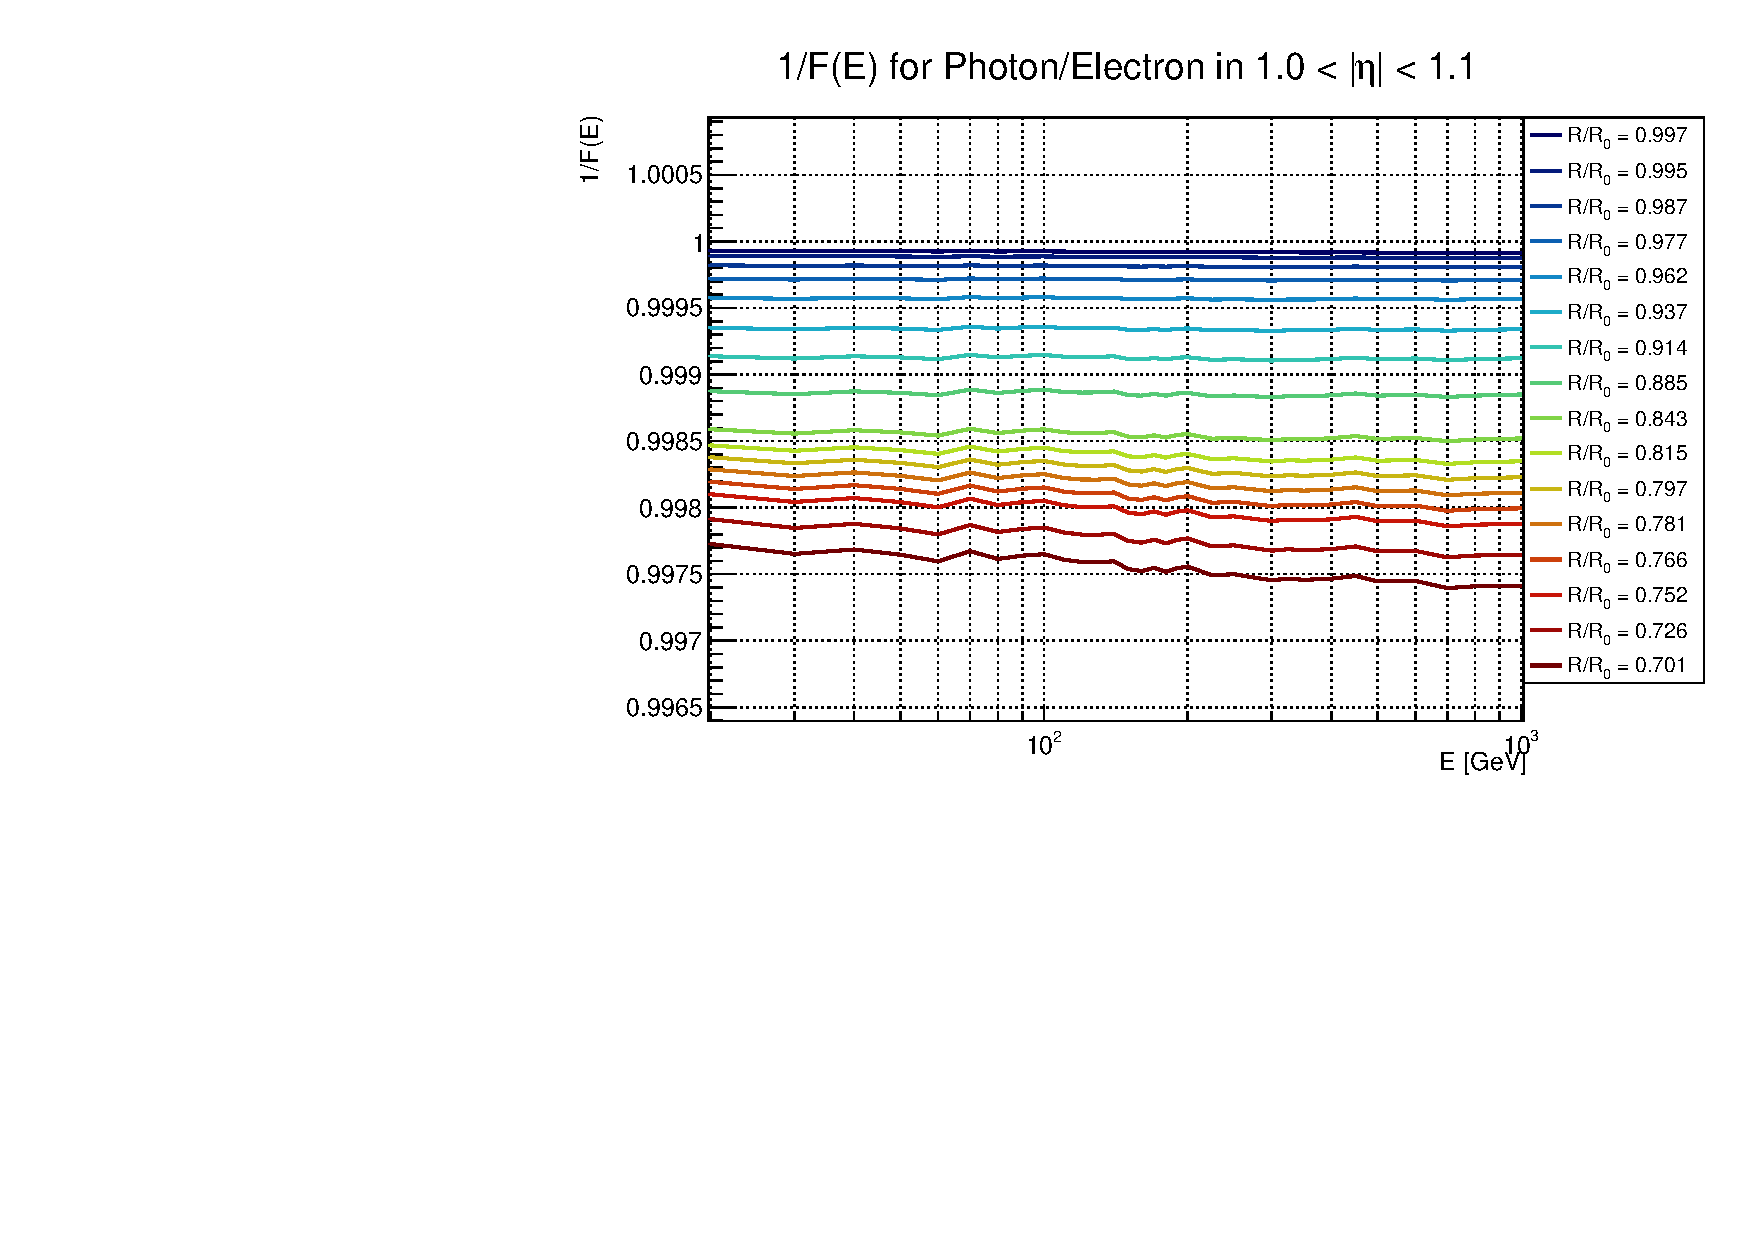
\includegraphics[width=\textwidth]{07-figures/F_vs_E_ratio_ring_10_inEB.pdf}
            \end{center}
        \end{minipage}
    }~\subfloat{%
        \begin{minipage}[t]{0.5\textwidth}%
            \begin{center}
                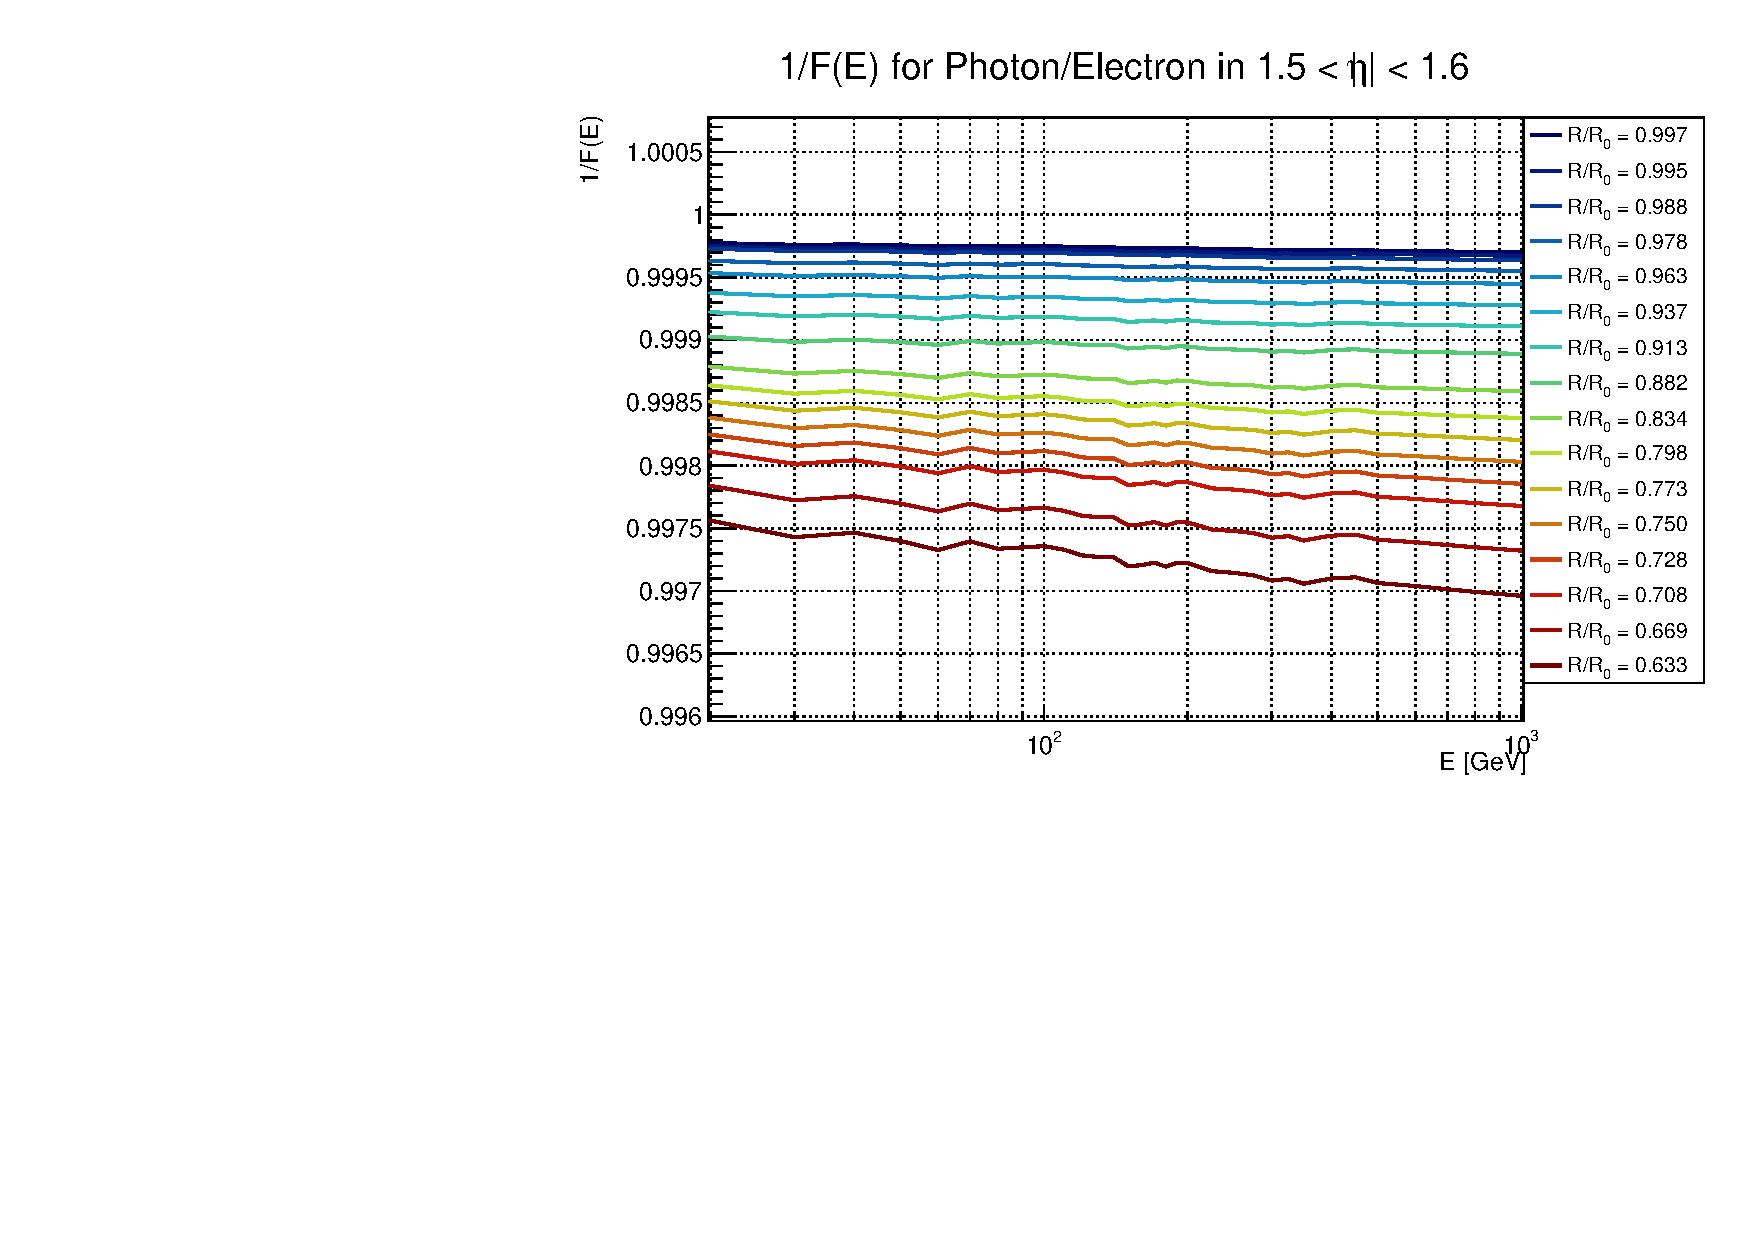
\includegraphics[width=\textwidth]{07-figures/F_vs_E_ratio_ring_15_inEE.pdf}
            \end{center}
        \end{minipage}
    }~\subfloat{%
        \begin{minipage}[t]{0.5\textwidth}%
            \begin{center}
                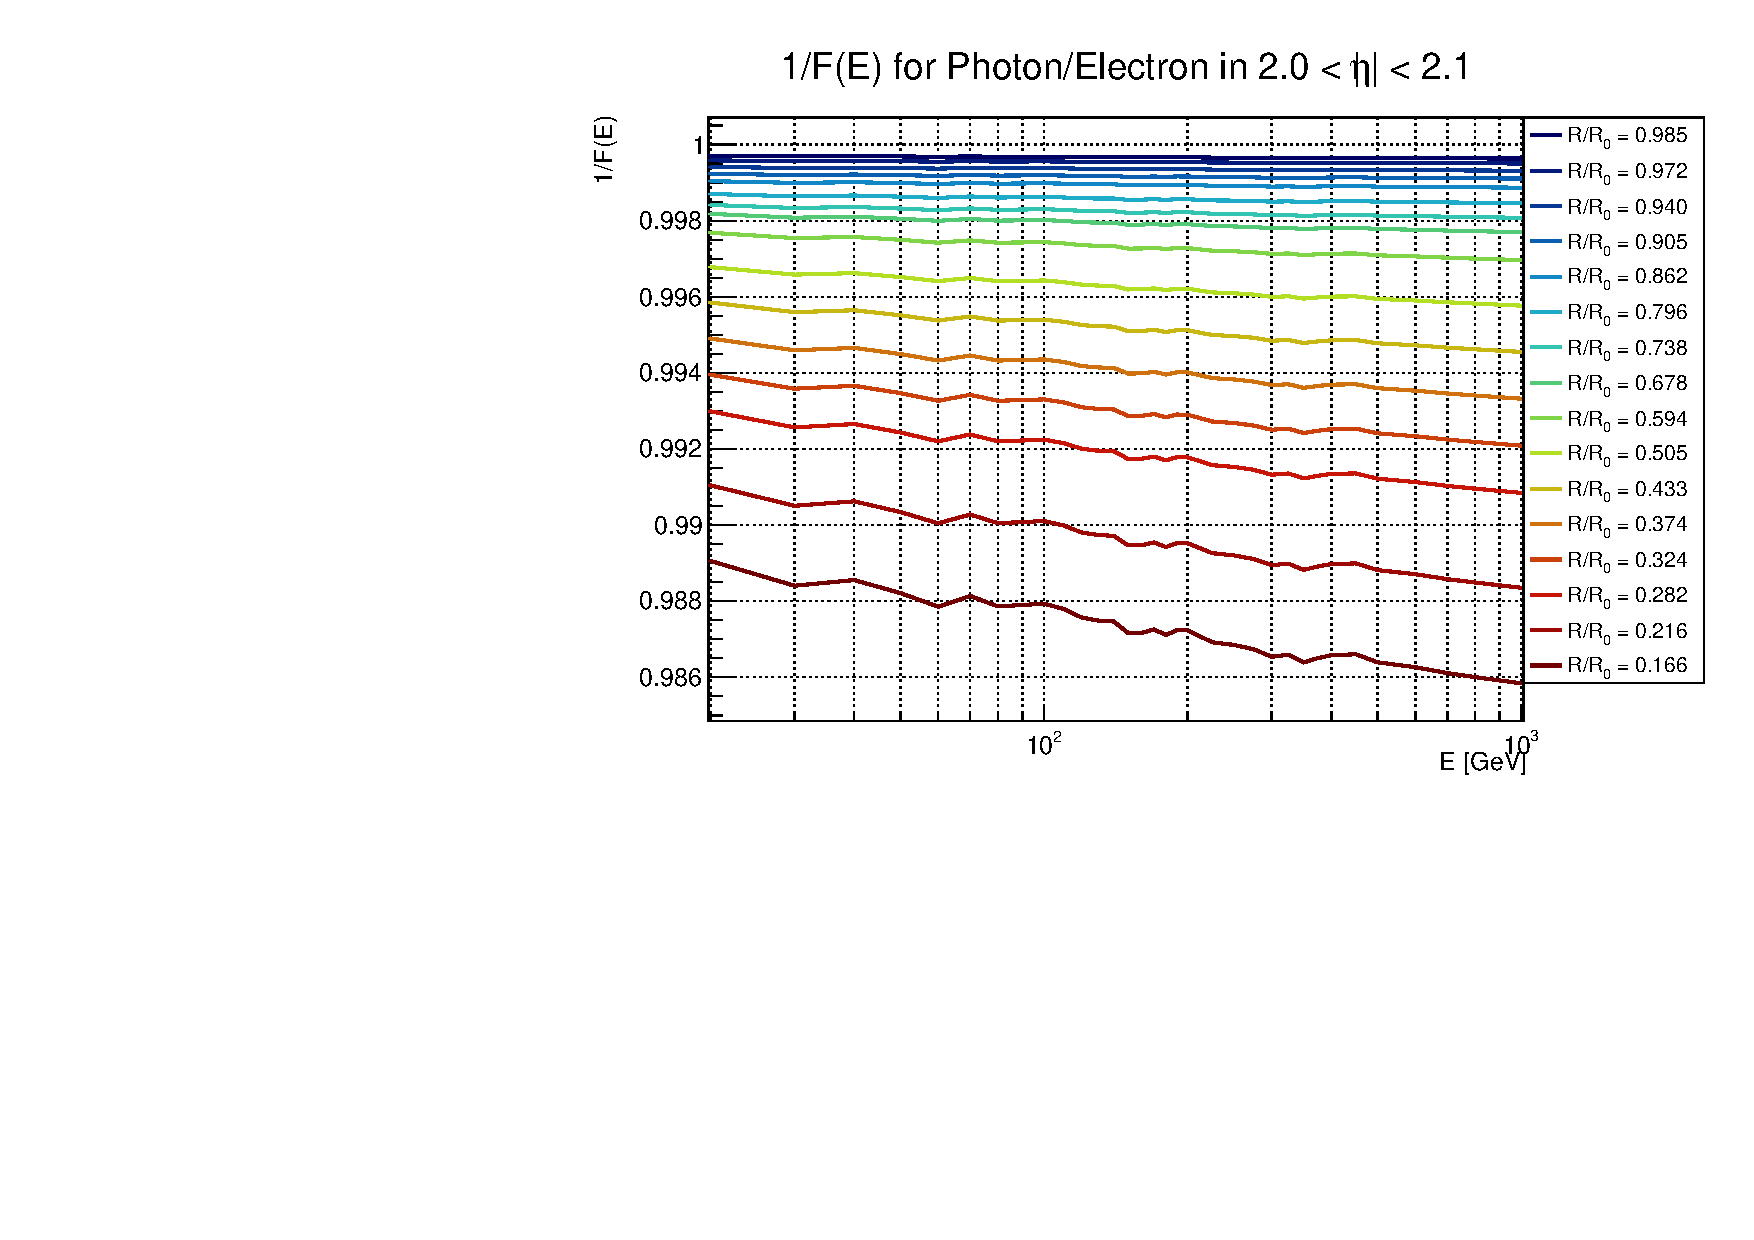
\includegraphics[width=\textwidth]{07-figures/F_vs_E_ratio_ring_20_inEE.pdf}
            \end{center}
        \end{minipage}
    }
    \caption[FNUF corrections vs. energy]{FNUF corrections as a function of energy for different value of |$\eta$| in the EB and EE taken from~\cite{fnuf_dps_note}.}
    \label{fig:fnuf_vs_energy}
\end{figure}

\begin{figure}[htbp!]
    \centering
    \includegraphics[width=0.5\textwidth]{07-figures/pho_ele_shower_profiles_lowR9.png}
    \caption[Shower maximum for electrons and photons with R$_9 < 0.96$]{The average depth of shower max for electrons (filled band) and photons (black) with R$_9 < 0.96$. The ratio pad shows good agreement, indicating that there is very little difference in the location of the shower maximum.}
    \label{fig:lowR9_shower_max}
\end{figure}


The agreement between the FLUKA+S-Litrani simulation and the data determines the uncertainty on the FNUF correction. The sources of this are:

\begin{itemize}
\item Luminosity modeling: The FLUKA simulation calculates $\mu_{\mathrm{ind}}$ assuming a constant instantaneous luminosity. This does not include in-fill and fill-to-fill variations in the luminosity. An uncertainty of 2\% in EB and 8\% in EE was derived using the spread of FNUF corrections in bins of $\eta$ to account for these variations in luminosity.

\item Agreement between the data and S-Litrani simulation: in \cite{NIM-A-564-2006} the light loss of proton-irradiated crystals with 0.1 m$^{-1}$ $< \mu_{\mathrm{ind}} < $ 10 m$^{-1}$ was measured using cosmic ray muons and compared with the S-Litrani simulation. The data and simulation agreed to within 20\%, and an uncertainty of 10\% in EB and 20\% in EE is assigned to cover ``imperfections" of simulation predictions for a given value of $\mu_{\mathrm{ind}}$. The value is higher in the EE due to the larger radiation dose, leading to larger values of $\mu_{\mathrm{ind}}$.

\item Changes in the of sensitivity of VPTs and APDs: The range of the effect of radiation on the EE VPT conditioning was measured to vary by up to 30\%~\cite{VPT-conditioning}. An uncertainty of 27\% in the EE is assigned to cover these variations. The effect of radiation on the APDs is to increase the dark current. This is tracked continuously and corrected for by increasing the applied bias voltage, so no uncertainty is needed in the EB. 

\item Spread in $\mu_{\mathrm{nat}}$ measurements: The ELM model assumes an initial value of $\mu_{\mathrm{nat}} = 0.3$ m$^{-1}$, however the initial measurements of $\mu_{\mathrm{nat}}$ ranged from 0.2 - 0.35 m$^{-1}$~\cite{mu_natural}. An uncertainty of 15\% is applied to the FNUF correction in EB and EE to account for this variation.   

\item Effect of ``PN-corrections" on laser measurements: A drift of 1\% every 10 fb$^{-1}$ is visible in the EB energy scale in the Run 2 dataset~\cite{CMS:ECALRun2}. This drift is not fully corrected by applying the laser corrections to the crystal energy calibration. The origin of this drift is not fully understood. Therefore the uncertainty associated with this effect is propagated directly to the mass measurement itself: 5~MeV for 2016 preVFP, 10~MeV for 2016 postVFP, 10~MeV for 2017, and 30~MeV for 2018.      
\end{itemize}

The total systematic uncertainty on the FNUF correction is 20\% in EB and 35\% in EE. Additionally, a systematic uncertainty of 5~MeV for 2016 preVFP, 10~MeV for 2016 postVFP, 10~MeV for 2017, and 30~MeV for 2018 is applied directly to the mass measurement. For additional details, see~\cite{FNUF1} and~\cite{FNUF_uncertainties}. 





%%%%%%%%%%%%%%%%%%%%%%%%%%%%%%%%%%%%%%%%%%%%%%%%%%%%%%%%%%%%%%%%%%%%%%%%%%%%%%%%%%%%%%%%%%
\subsubsection{Uncertainty from shower shape modeling}

The uncertainty due to imperfect modeling of the shower shape for both photons and electrons in the simulation is estimated using Z$\rightarrow$ee and H$\rightarrow\gamma\gamma$ Monte Carlo samples with and without shower shape corrections. After the shower shape correction is applied, the energy regression is re-run. The e/$\gamma$ double ratio of the difference with and without the correction is taken as an estimate of the systematic uncertainty. Results are summarized in Table~\ref{tab:shower_shape_unc} for different photon categories in $\eta$ and R$_9$. Due to the improved agreement of the shower shape variables between Legacy 2016 data and simulation, this uncertainty is less than in our previous measurement.

\begin{table}[h]
    \centering
    \begin{tabular}{|c|c|}
        \hline
        \textbf{Photon category} & \textbf{e/$\gamma$ relative scale unc.} ($\times 10^{-2}$)  \\ \hline
         EB R$_9 > 0.94$, $|\eta| < 1$ & -0.01 \\
         EB R$_9 > 0.94$, $|\eta| > 1$ & -0.00 \\
         EB R$_9 < 0.94$, $|\eta| < 1$ & -0.00 \\
         EB R$_9 < 0.94$, $|\eta| > 1$ & -0.00 \\ \hline
         EE R$_9 > 0.94$, $|\eta| < 2$ & -0.02 \\
         EE R$_9 > 0.94$, $|\eta| > 2$ & -0.02 \\
         EE R$_9 < 0.94$, $|\eta| < 2$ & -0.00 \\
         EE R$_9 < 0.94$, $|\eta| > 2$ & -0.00 \\ \hline
         
    \end{tabular}
    \caption[Shower shape uncertainties]{Energy scale uncertainties associated with the imperfect modeling of the shower shape for the different classes of photons expressed in percent.}
    \label{tab:shower_shape_unc}
\end{table}


\section{Final models}

The final signal and background models with all uncertainties accounted for are presented in this section. The signal models in each of the five categories for each of the four datasets are shown in Figures~\ref{fig:signal_model_2016_preVFP}-~\ref{fig:signal_model_2018} and their background models can be seen in Figures~\ref{fig:bkg_model_2016_preVFP}-~\ref{fig:bkg_model_2018}. The combined signal and background models are shown in Figure~\ref{fig:model_run2}, and the expected yields in each category are shown in Table~\ref{tab:yields}


\begin{figure}[htbp!]
    \subfloat{%
        \begin{minipage}[t]{0.5\textwidth}%
            \begin{center}
                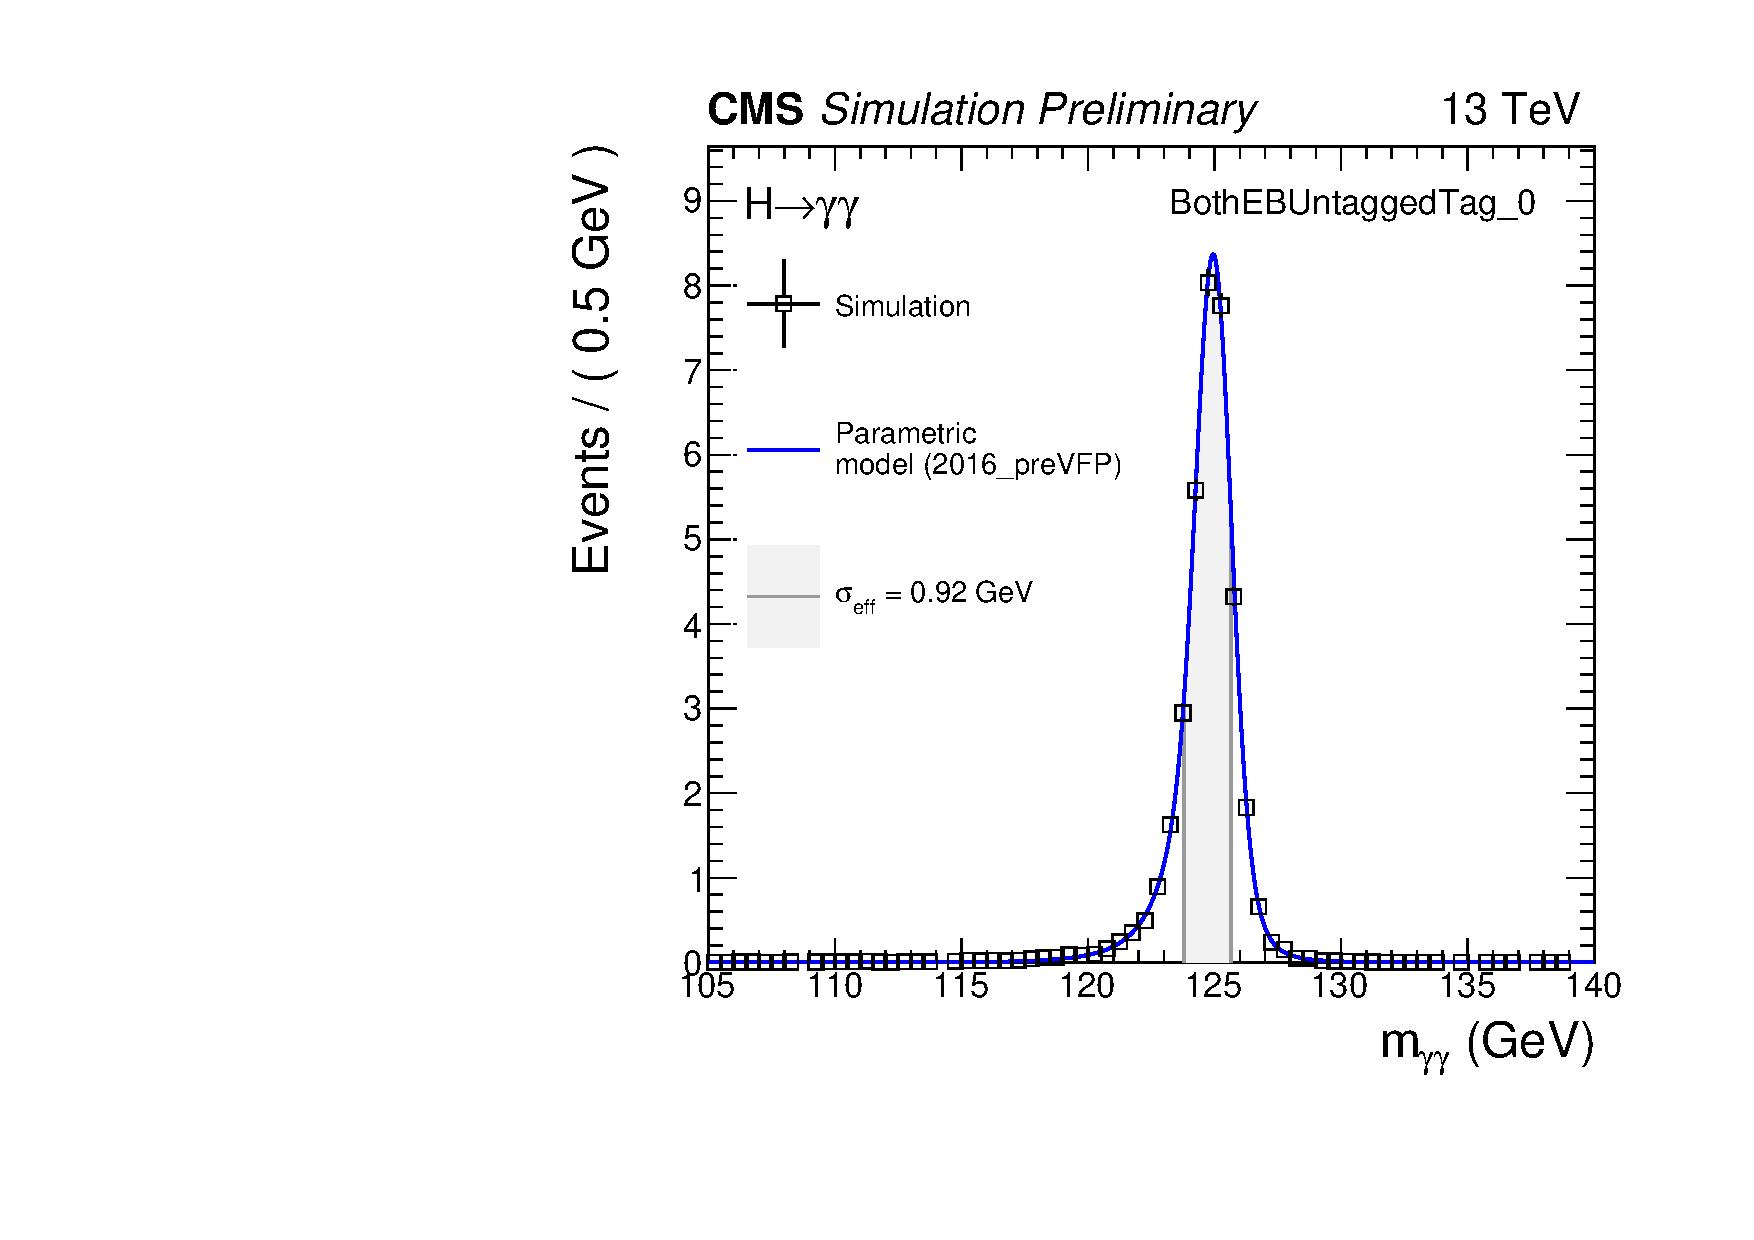
\includegraphics[width=\textwidth]{07-figures/signal_models/smodel_BothEBUntaggedTag_0_2016_preVFP.pdf}
            \end{center}
        \end{minipage}
    }~\subfloat{%
        \begin{minipage}[t]{0.5\textwidth}%
            \begin{center}
                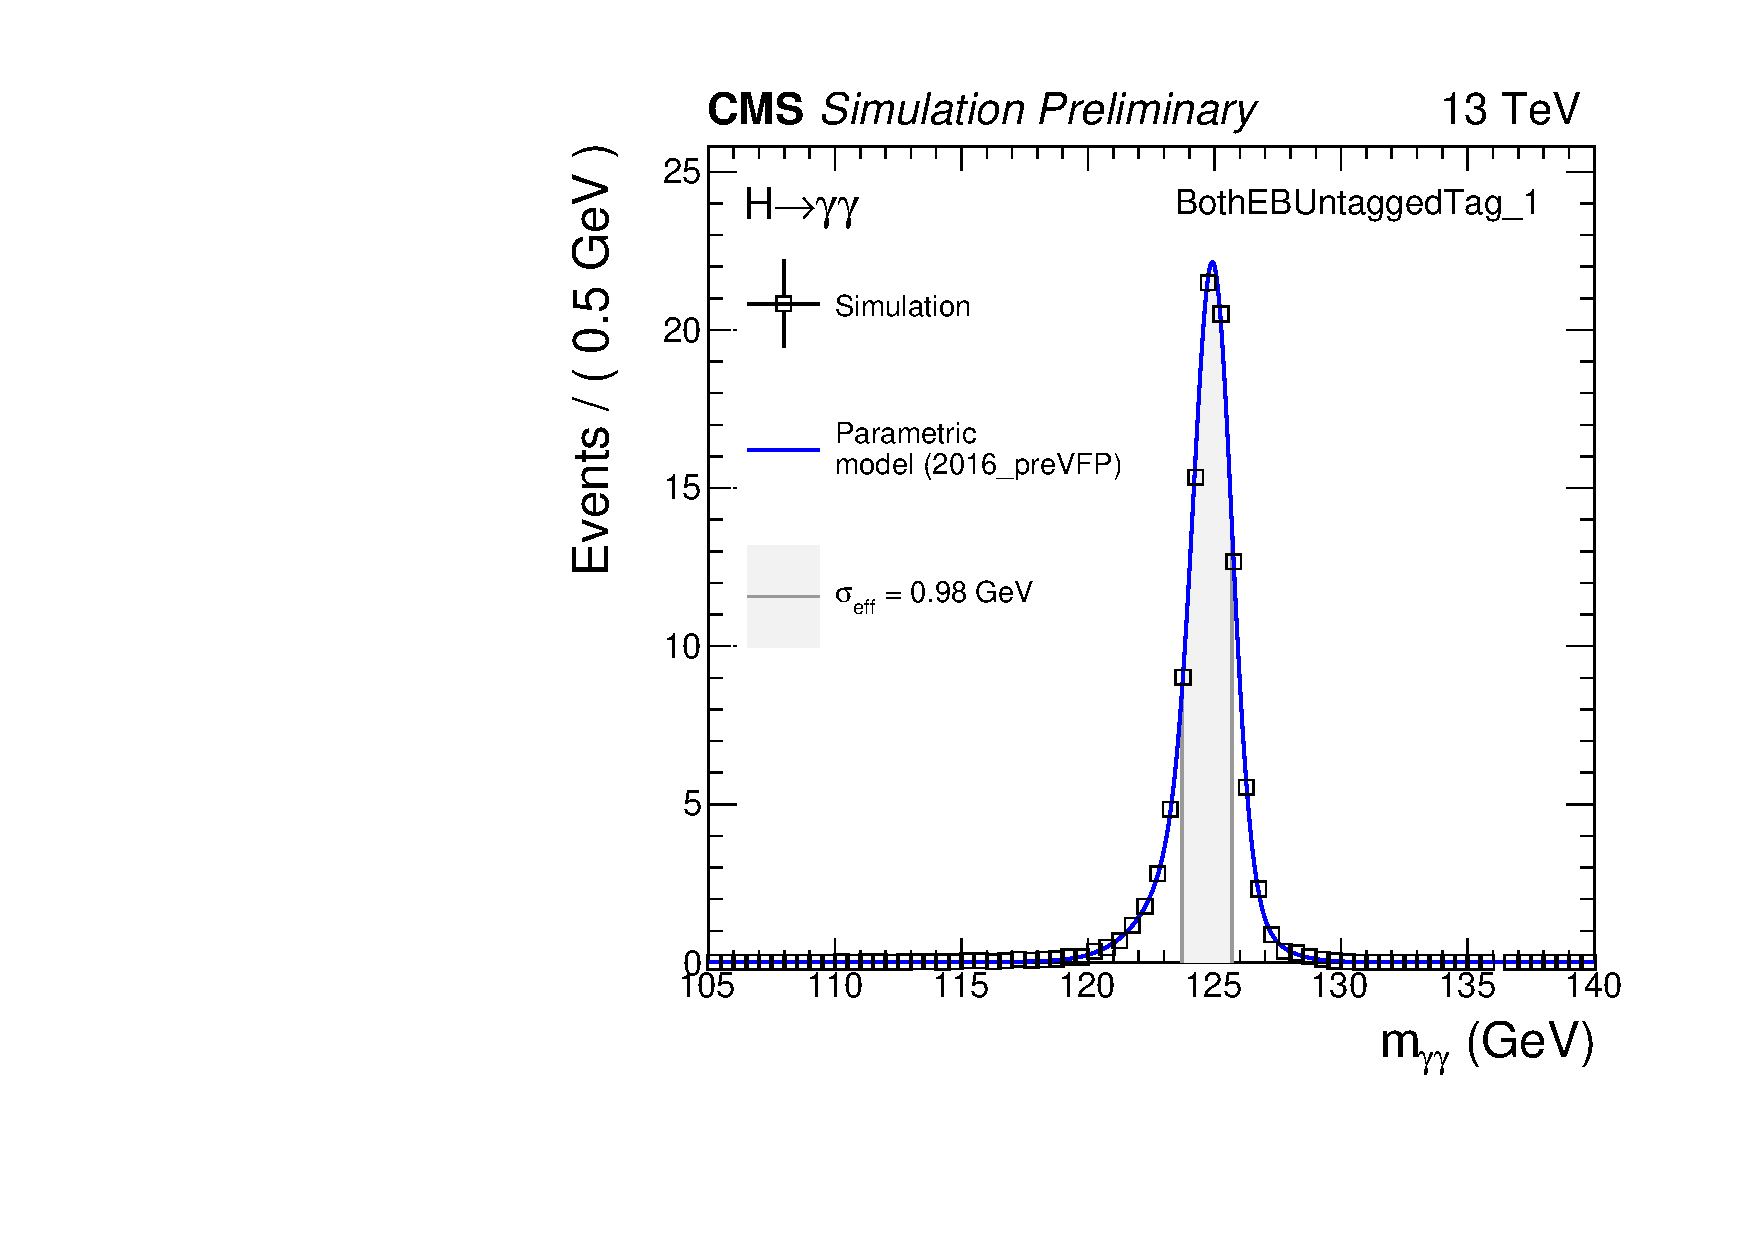
\includegraphics[width=\textwidth]{07-figures/signal_models/smodel_BothEBUntaggedTag_1_2016_preVFP.pdf}
            \end{center}
        \end{minipage}
    }~\subfloat{%
        \begin{minipage}[t]{0.5\textwidth}%
            \begin{center}
                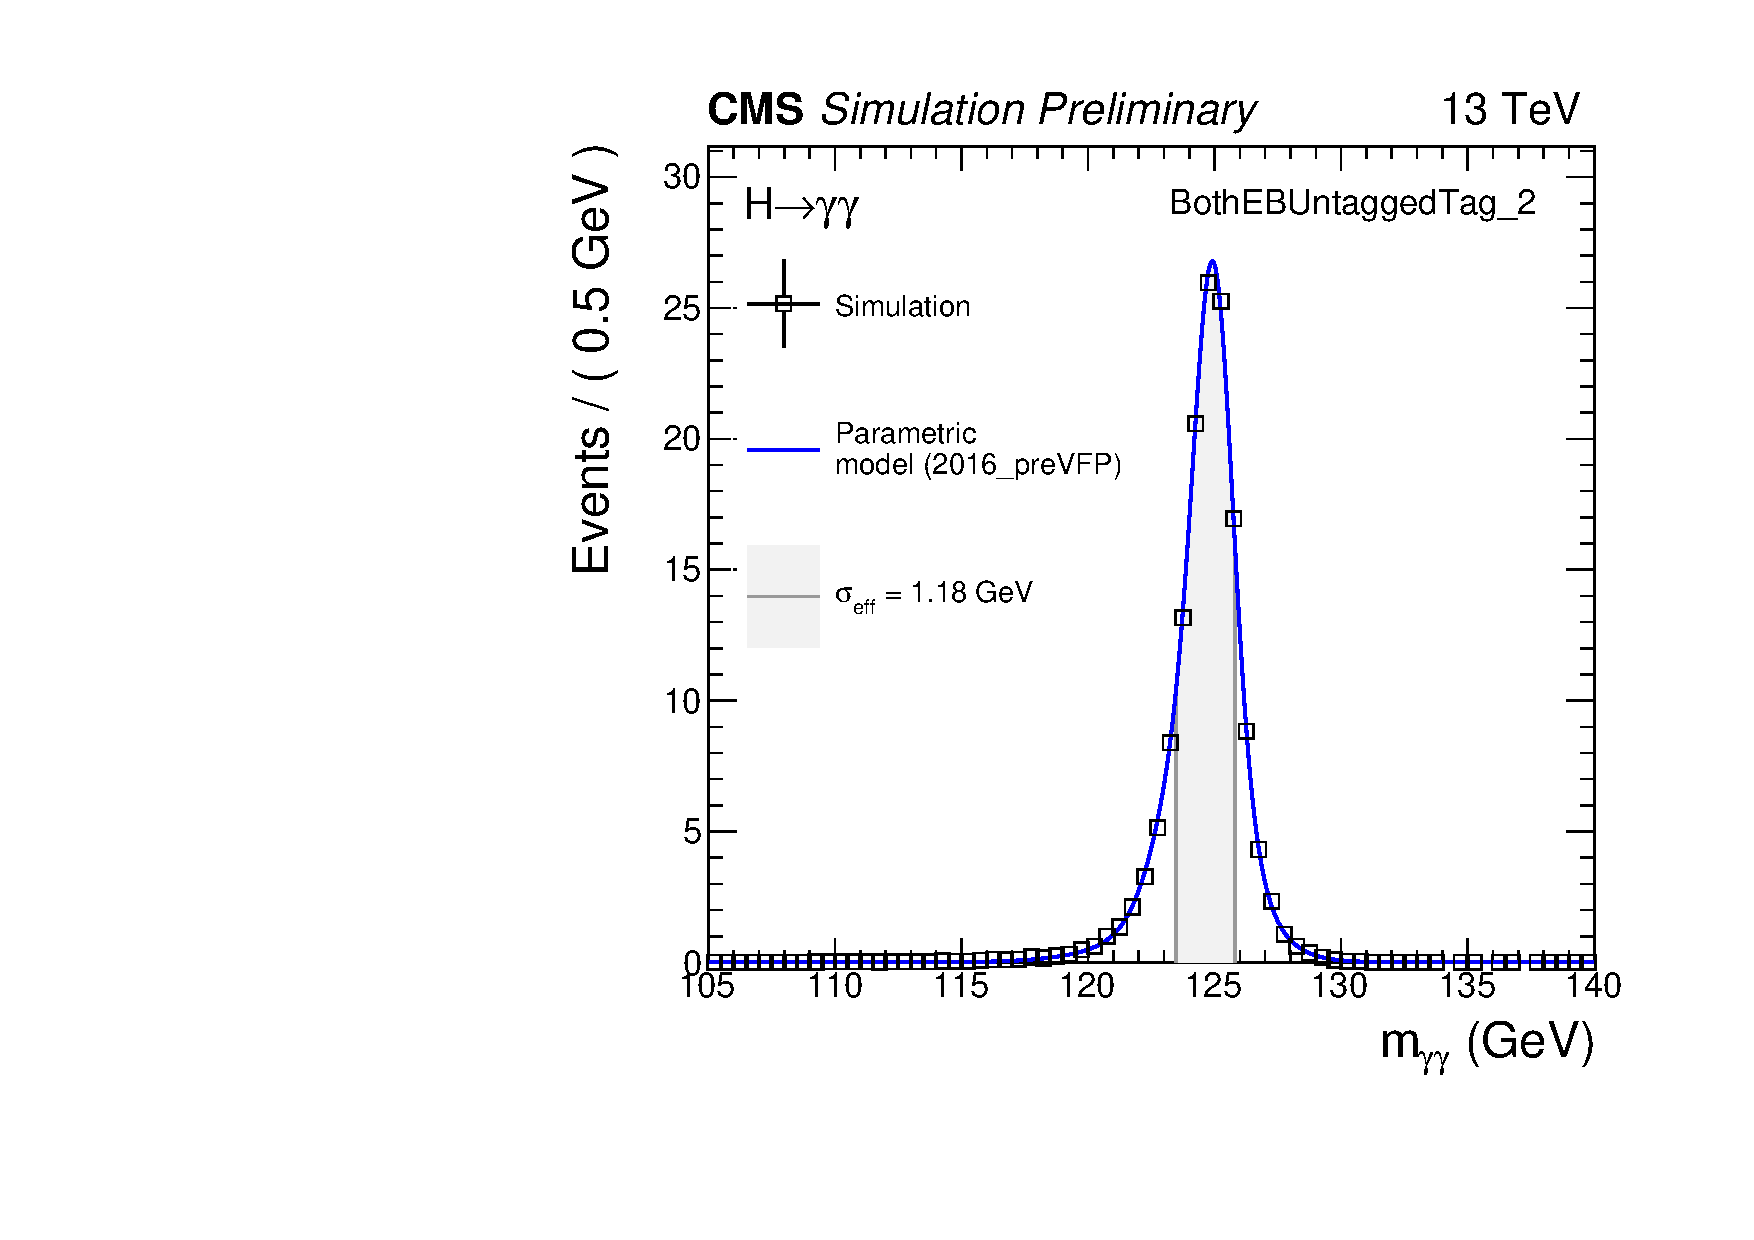
\includegraphics[width=\textwidth]{07-figures/signal_models/smodel_BothEBUntaggedTag_2_2016_preVFP.pdf}
            \end{center}
        \end{minipage}
    }~\subfloat{%
        \begin{minipage}[t]{0.5\textwidth}%
            \begin{center}
                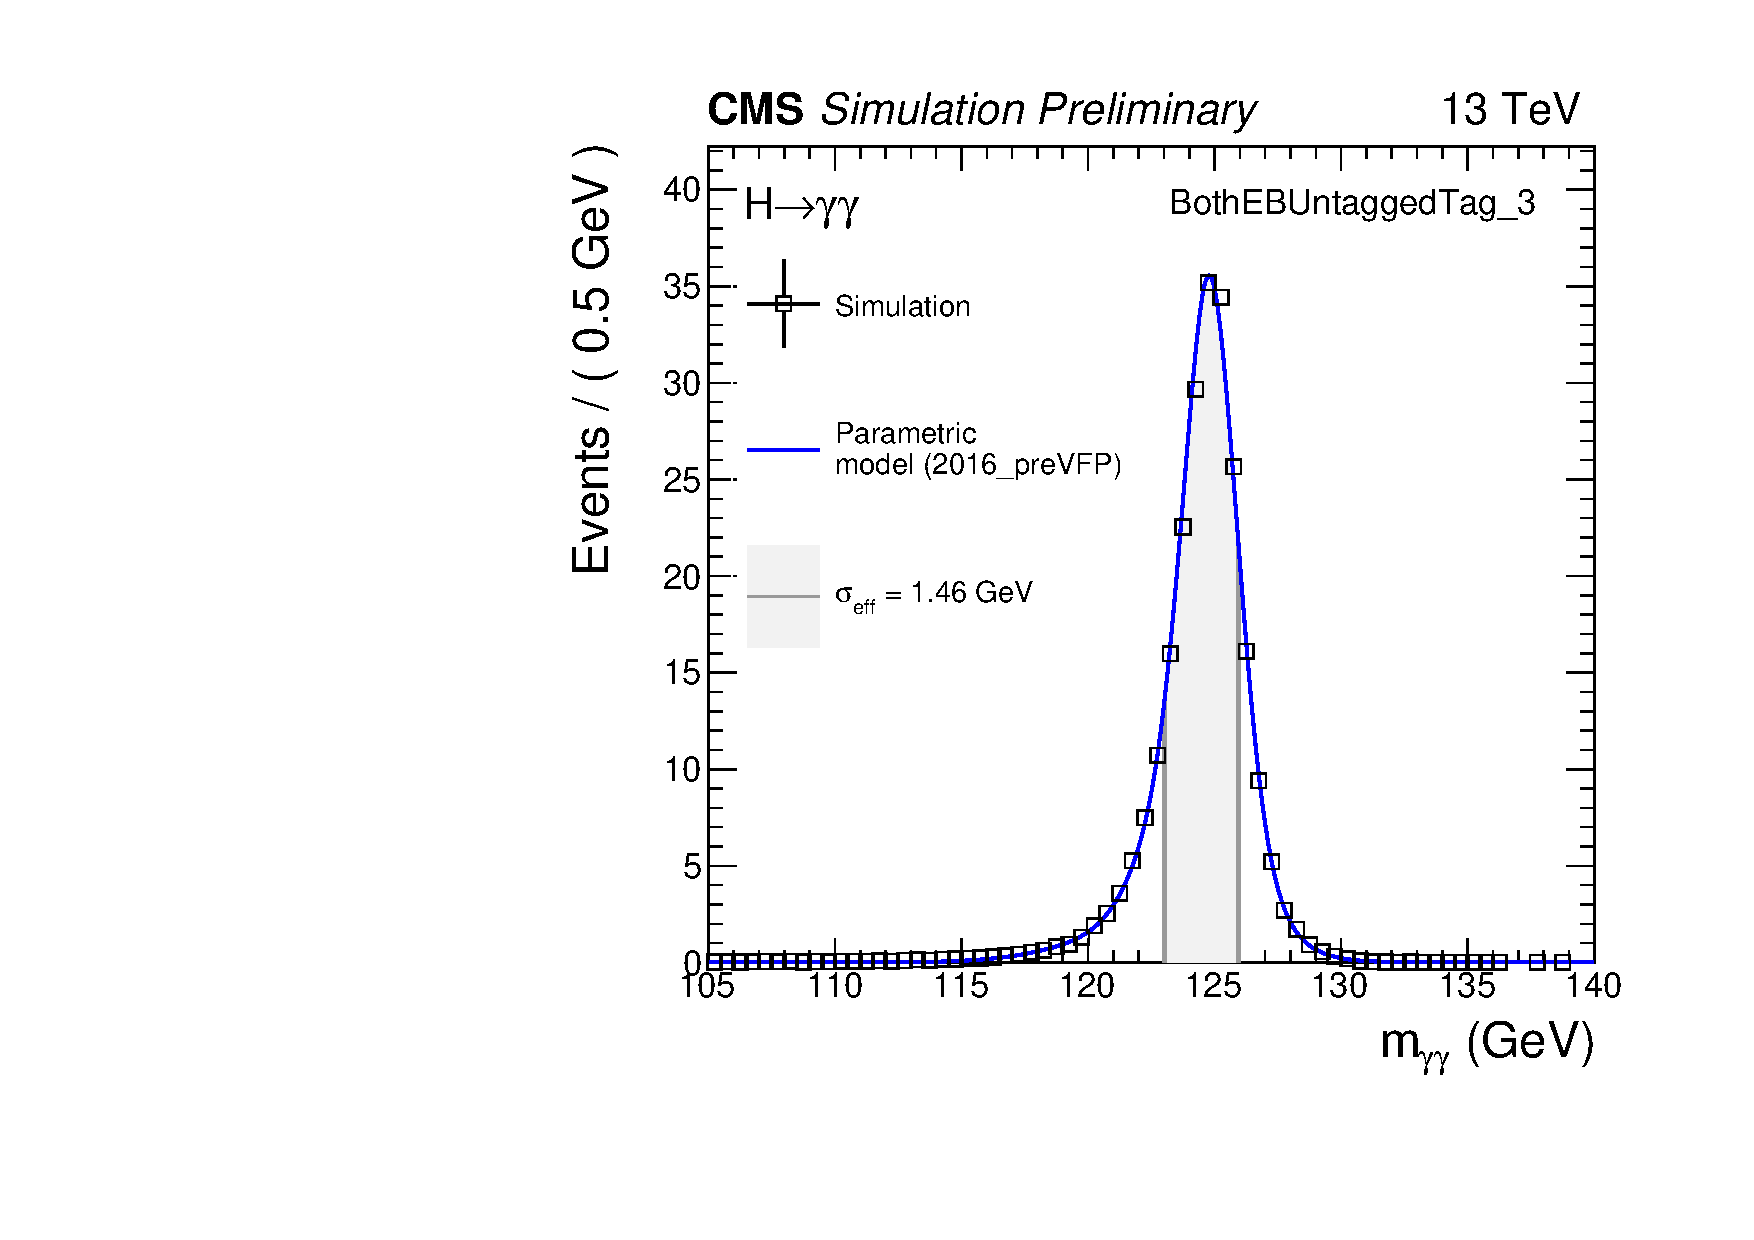
\includegraphics[width=\textwidth]{07-figures/signal_models/smodel_BothEBUntaggedTag_3_2016_preVFP.pdf}
            \end{center}
        \end{minipage}
    }~\subfloat{%
        \begin{minipage}[t]{0.5\textwidth}%
            \begin{center}
                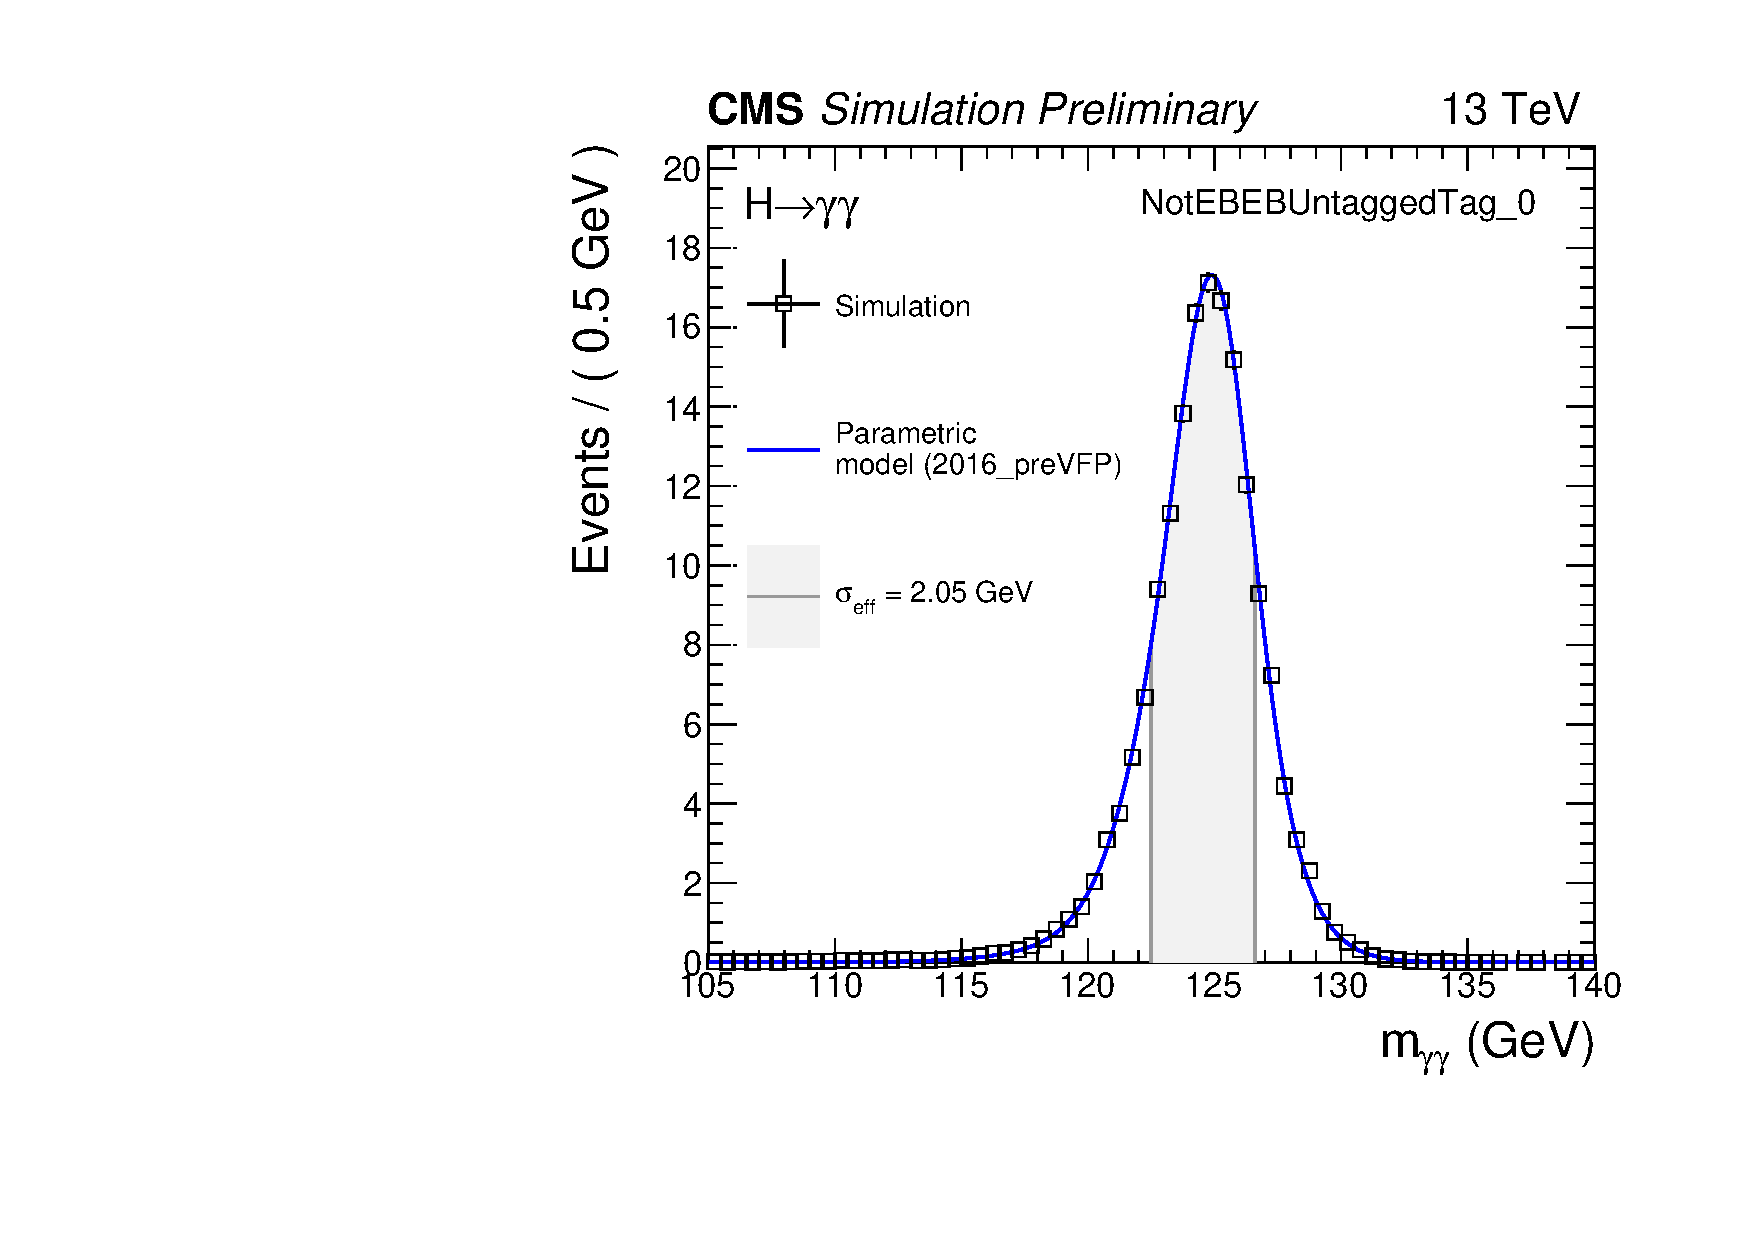
\includegraphics[width=\textwidth]{07-figures/signal_models/smodel_NotEBEBUntaggedTag_0_2016_preVFP.pdf}
            \end{center}
        \end{minipage}
    }~\subfloat{%
        \begin{minipage}[t]{0.5\textwidth}%
            \begin{center}
                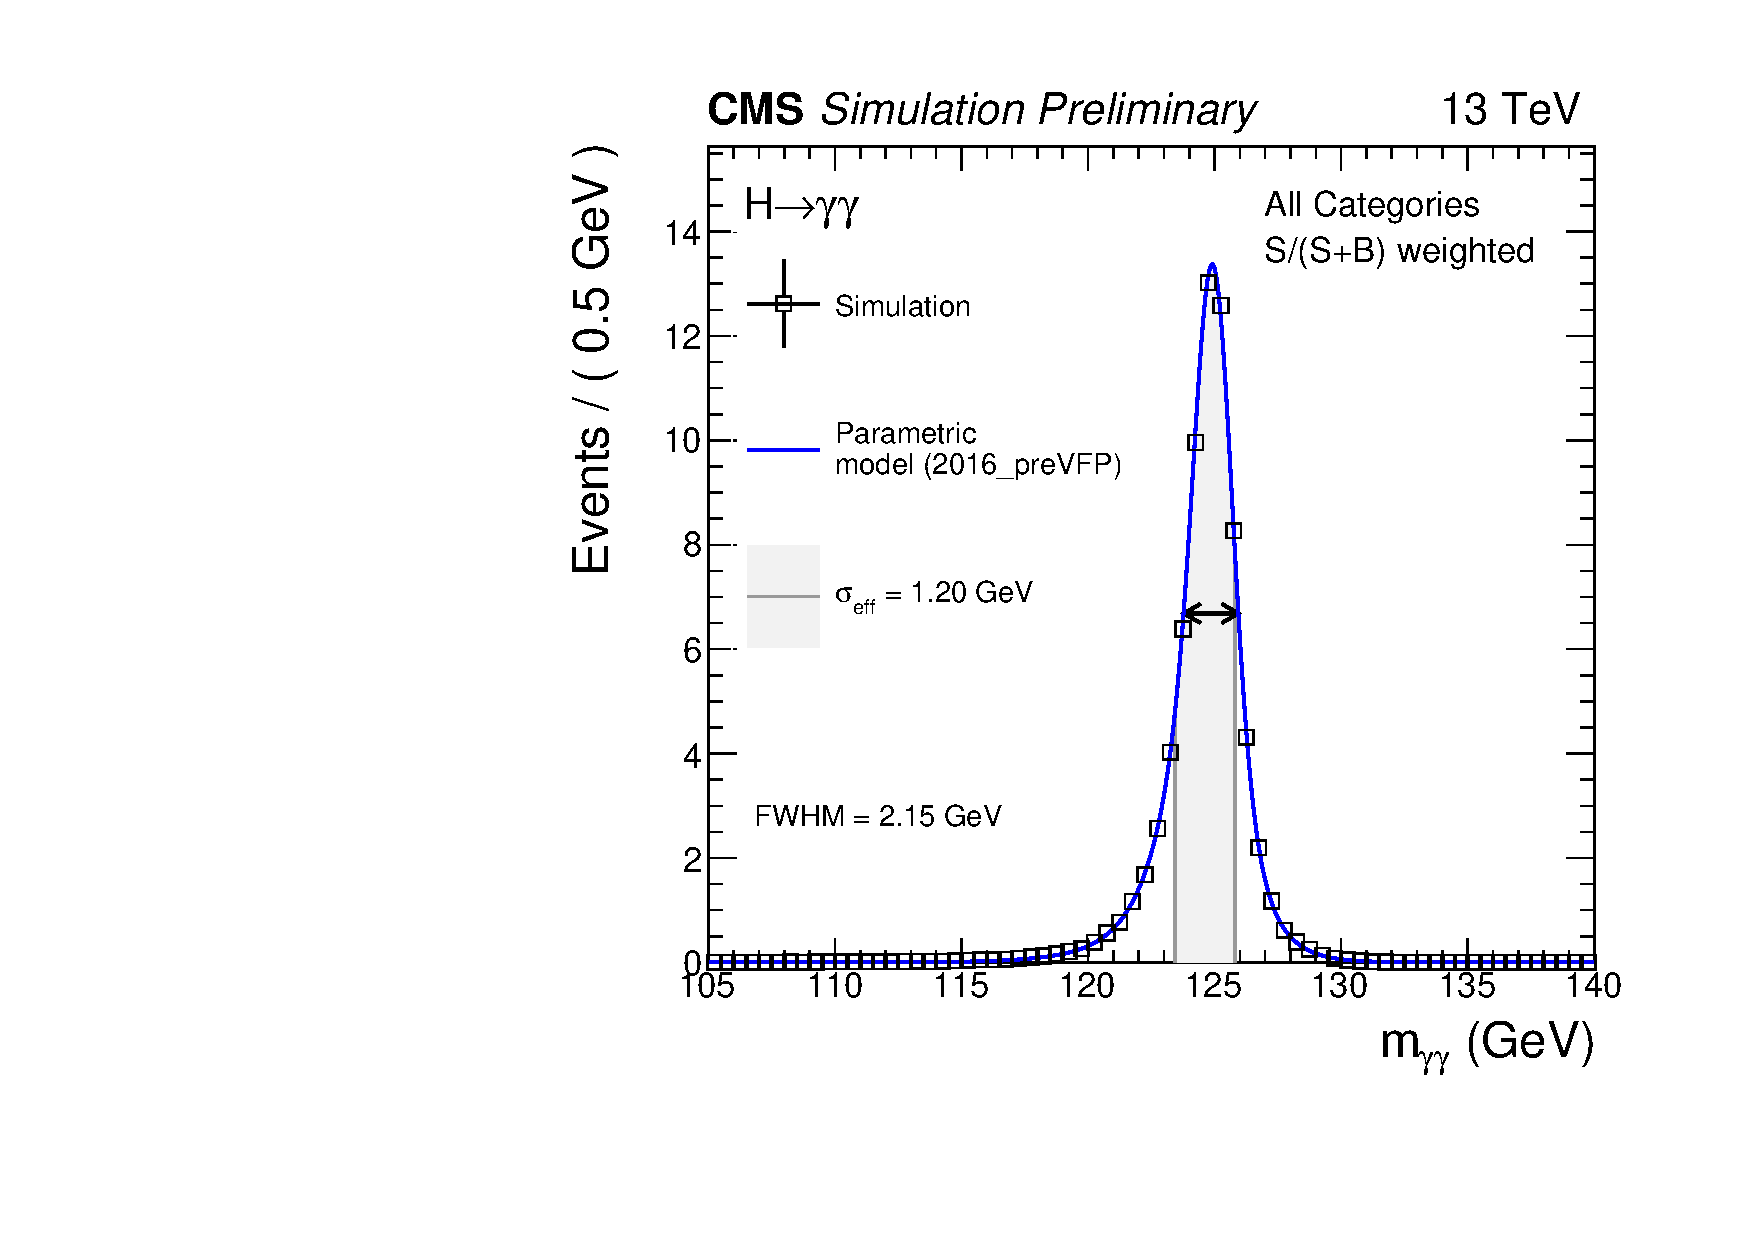
\includegraphics[width=\textwidth]{07-figures/signal_models/smodel_wall_2016_preVFP.pdf}
            \end{center}
        \end{minipage}
    }
    \caption[Signal models: 2016 preVFP]{Signal models for 2016 preVFP in each category and all categories combined.}
    \label{fig:signal_model_2016_preVFP}
\end{figure}

\begin{figure}[htbp!]
    \subfloat{%
        \begin{minipage}[t]{0.5\textwidth}%
            \begin{center}
                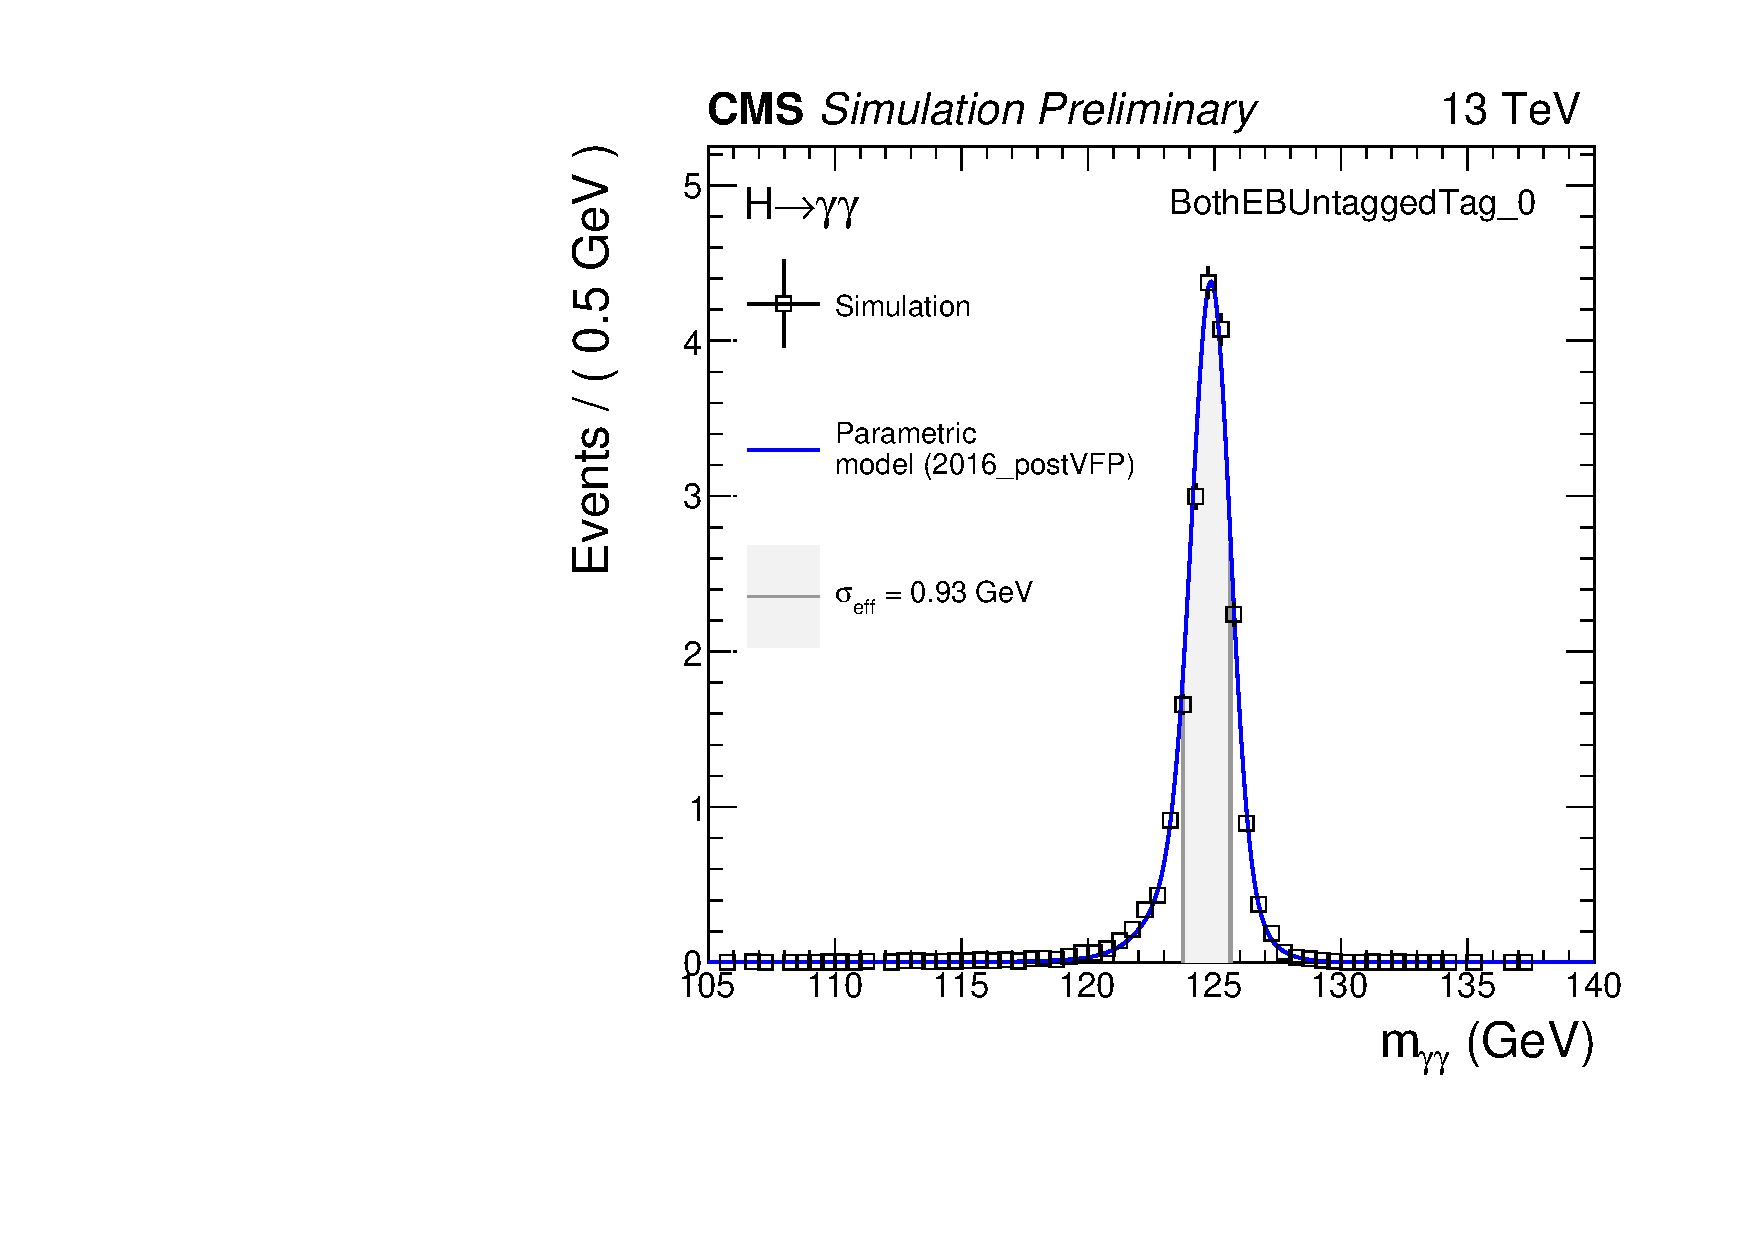
\includegraphics[width=\textwidth]{07-figures/signal_models/smodel_BothEBUntaggedTag_0_2016_postVFP.pdf}
            \end{center}
        \end{minipage}
    }~\subfloat{%
        \begin{minipage}[t]{0.5\textwidth}%
            \begin{center}
                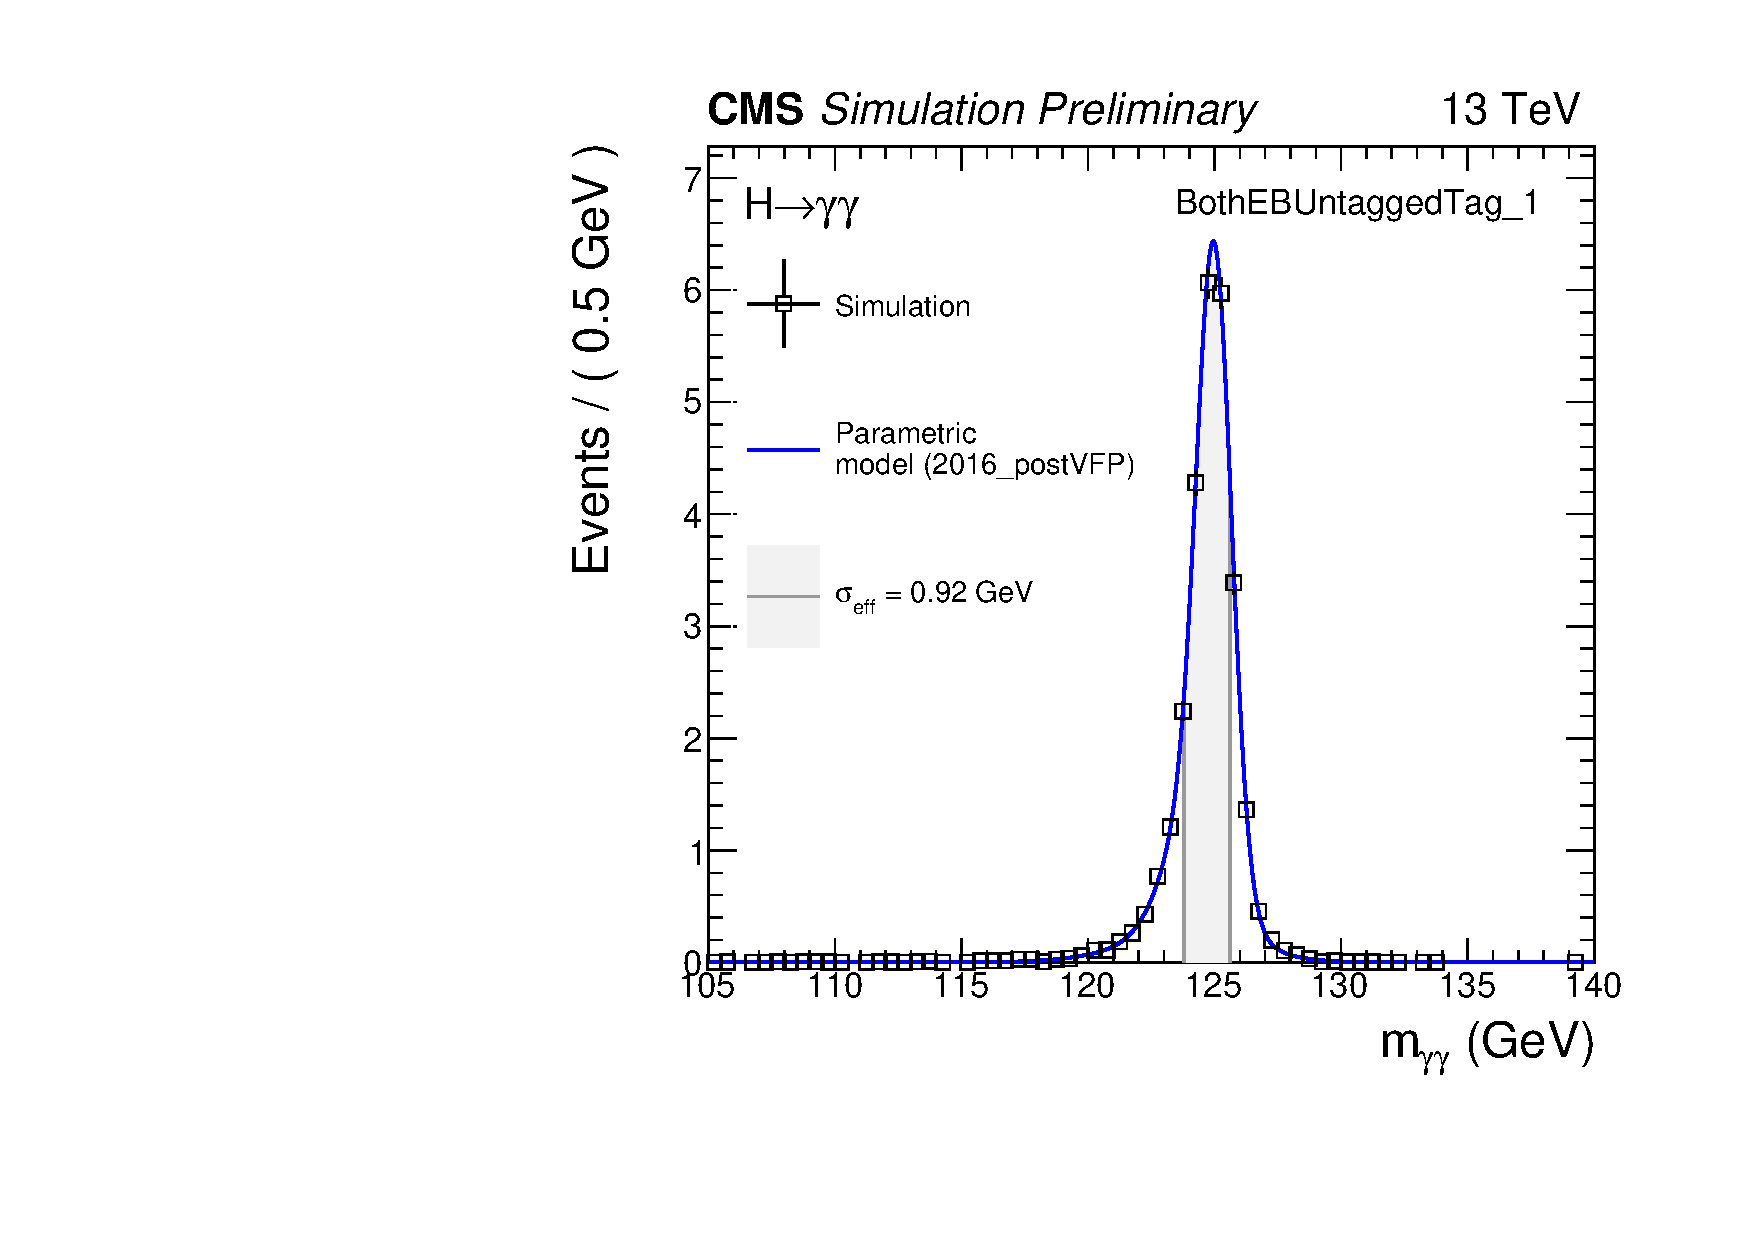
\includegraphics[width=\textwidth]{07-figures/signal_models/smodel_BothEBUntaggedTag_1_2016_postVFP.pdf}
            \end{center}
        \end{minipage}
    }~\subfloat{%
        \begin{minipage}[t]{0.5\textwidth}%
            \begin{center}
                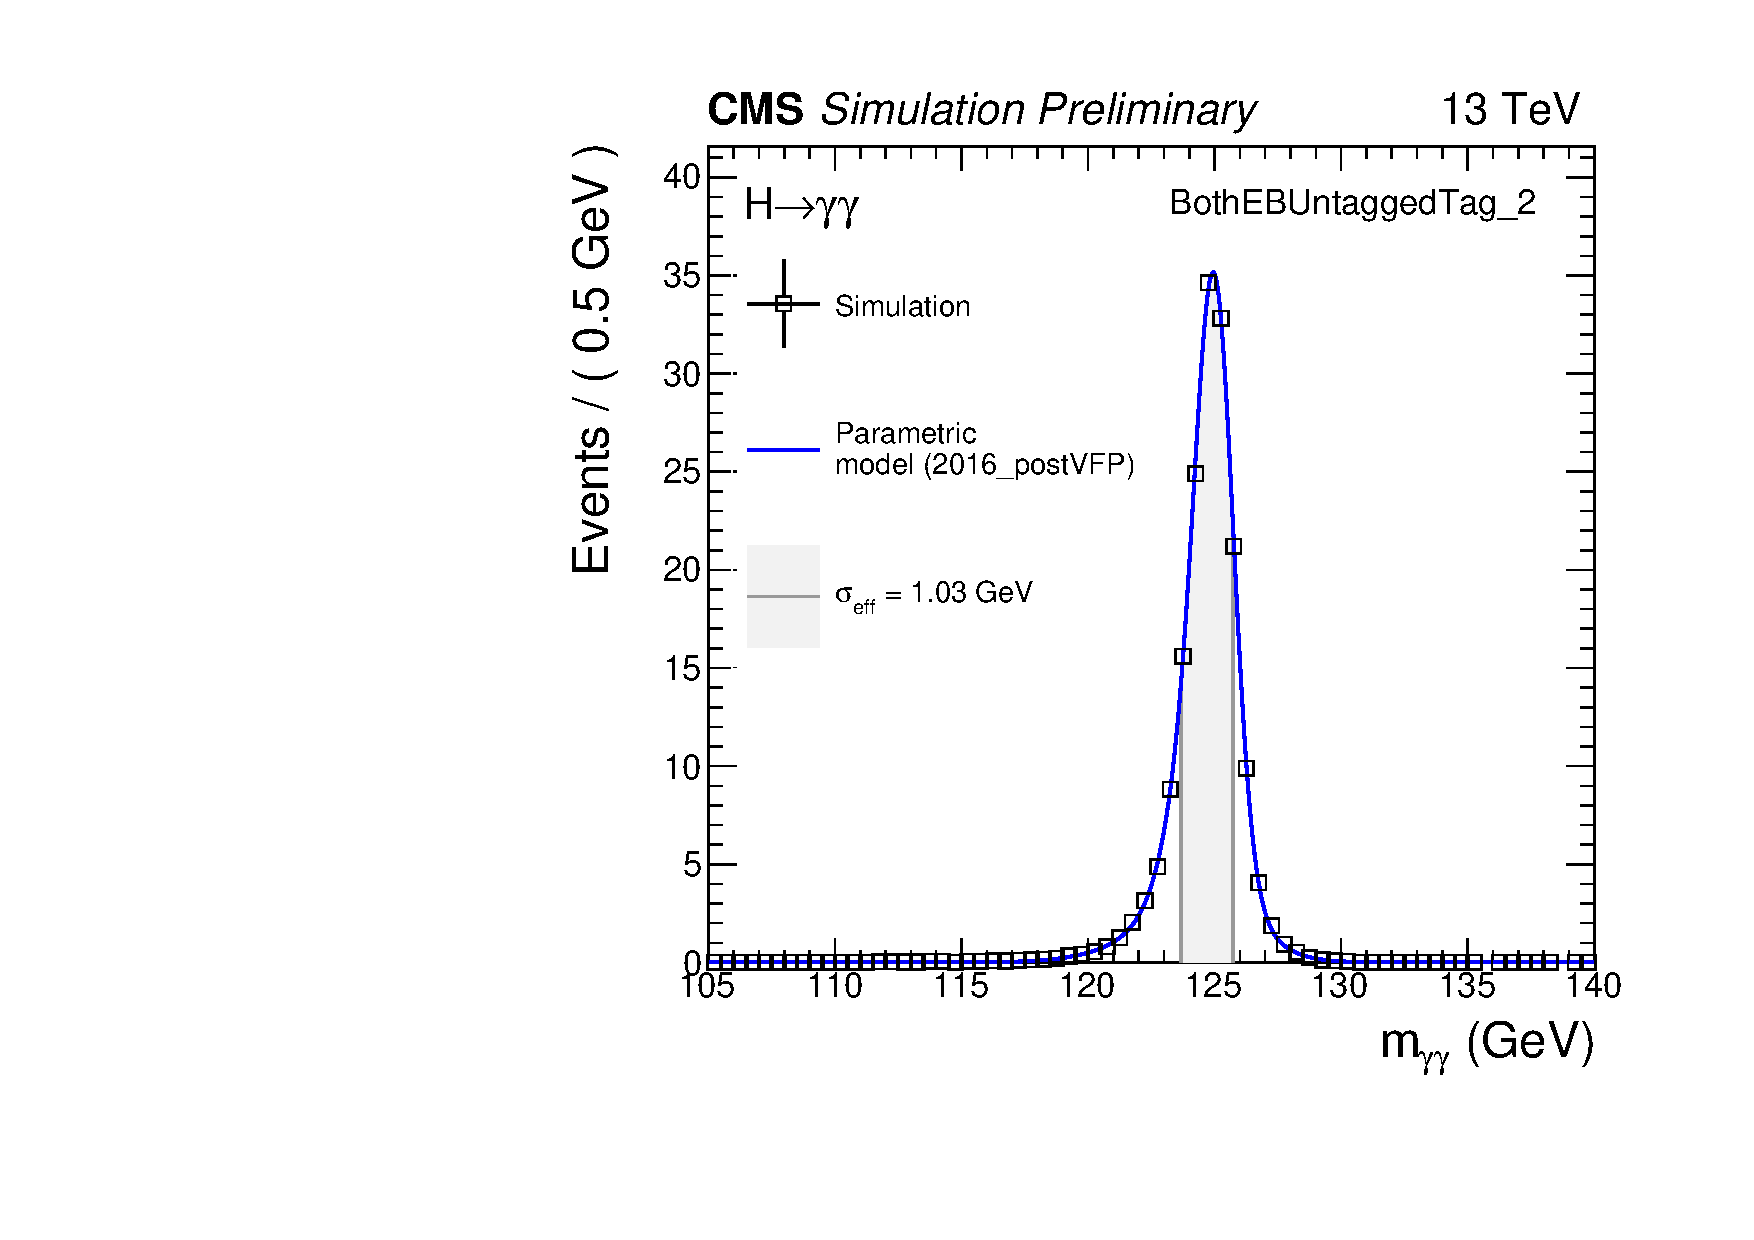
\includegraphics[width=\textwidth]{07-figures/signal_models/smodel_BothEBUntaggedTag_2_2016_postVFP.pdf}
            \end{center}
        \end{minipage}
    }~\subfloat{%
        \begin{minipage}[t]{0.5\textwidth}%
            \begin{center}
                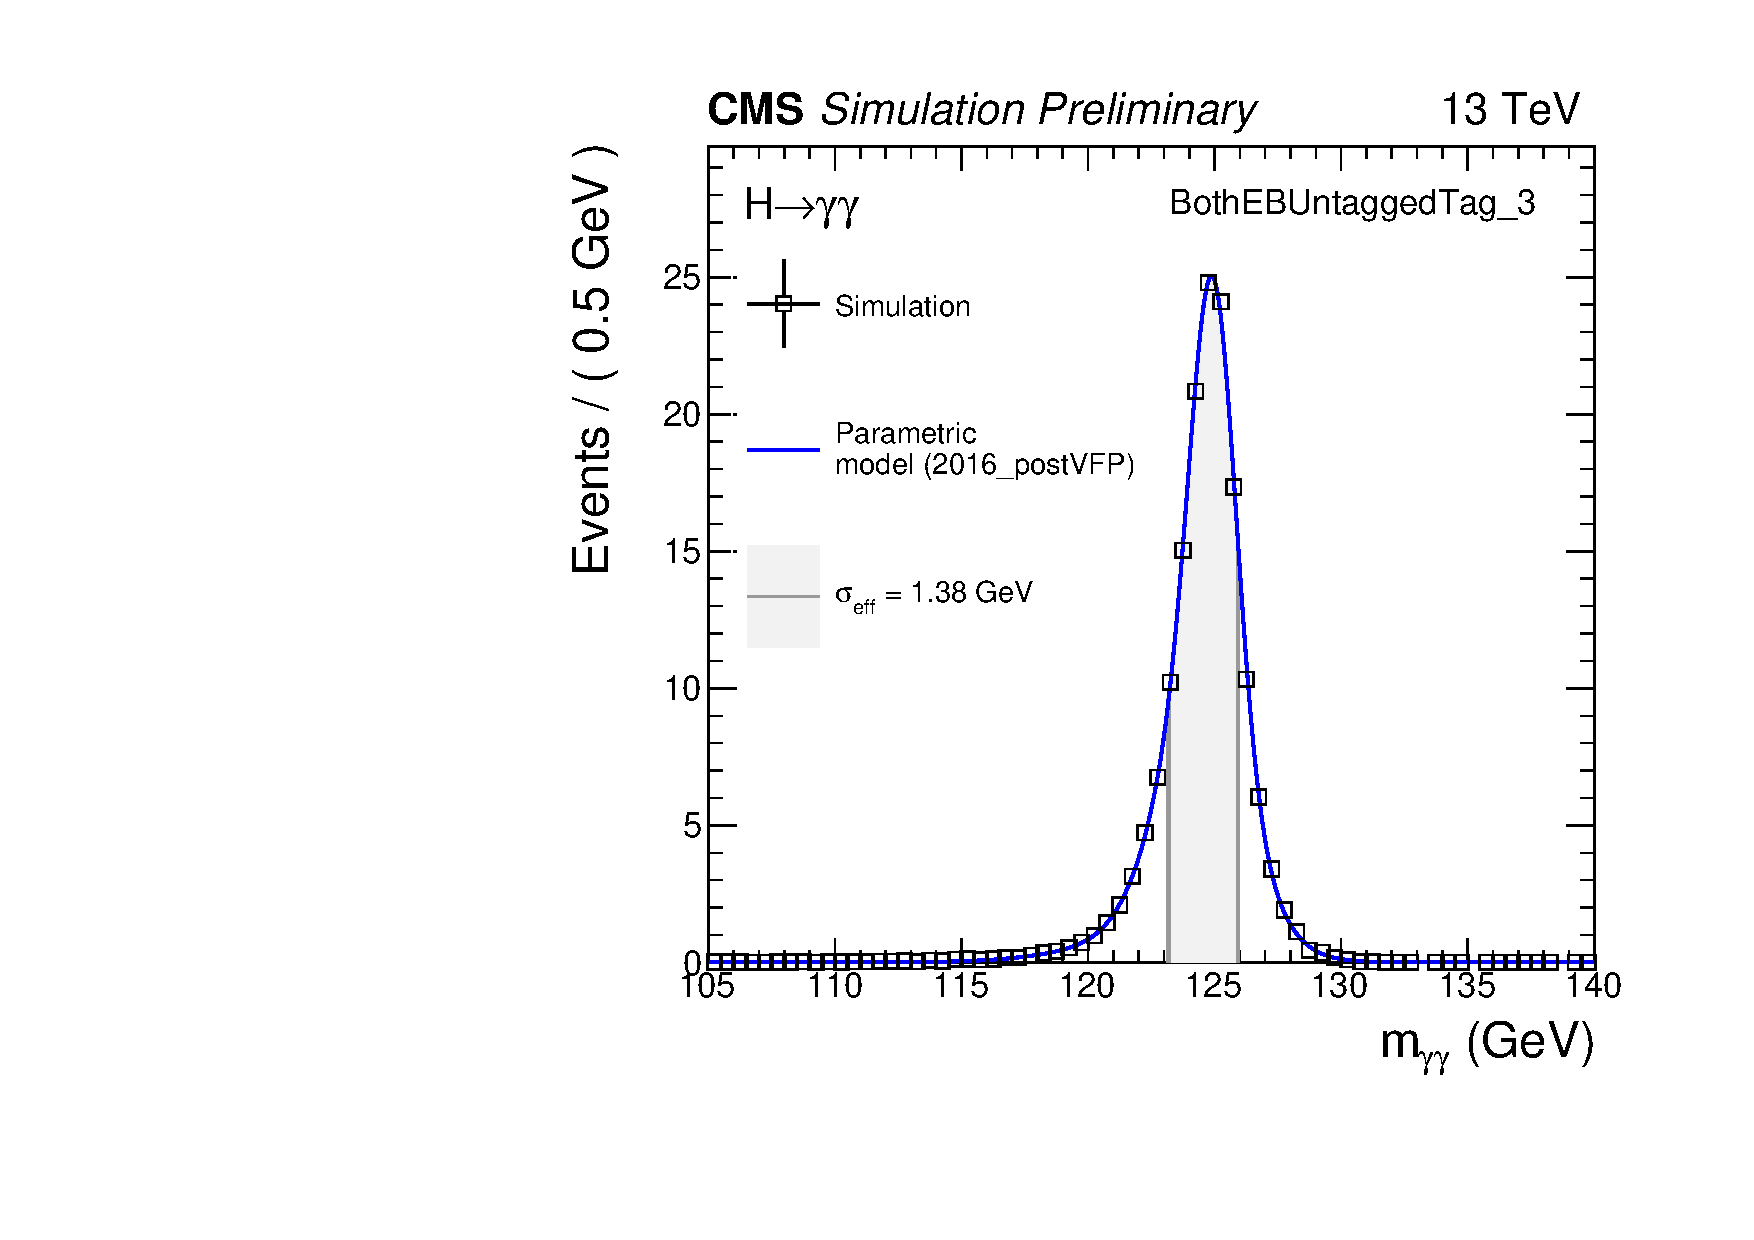
\includegraphics[width=\textwidth]{07-figures/signal_models/smodel_BothEBUntaggedTag_3_2016_postVFP.pdf}
            \end{center}
        \end{minipage}
    }~\subfloat{%
        \begin{minipage}[t]{0.5\textwidth}%
            \begin{center}
                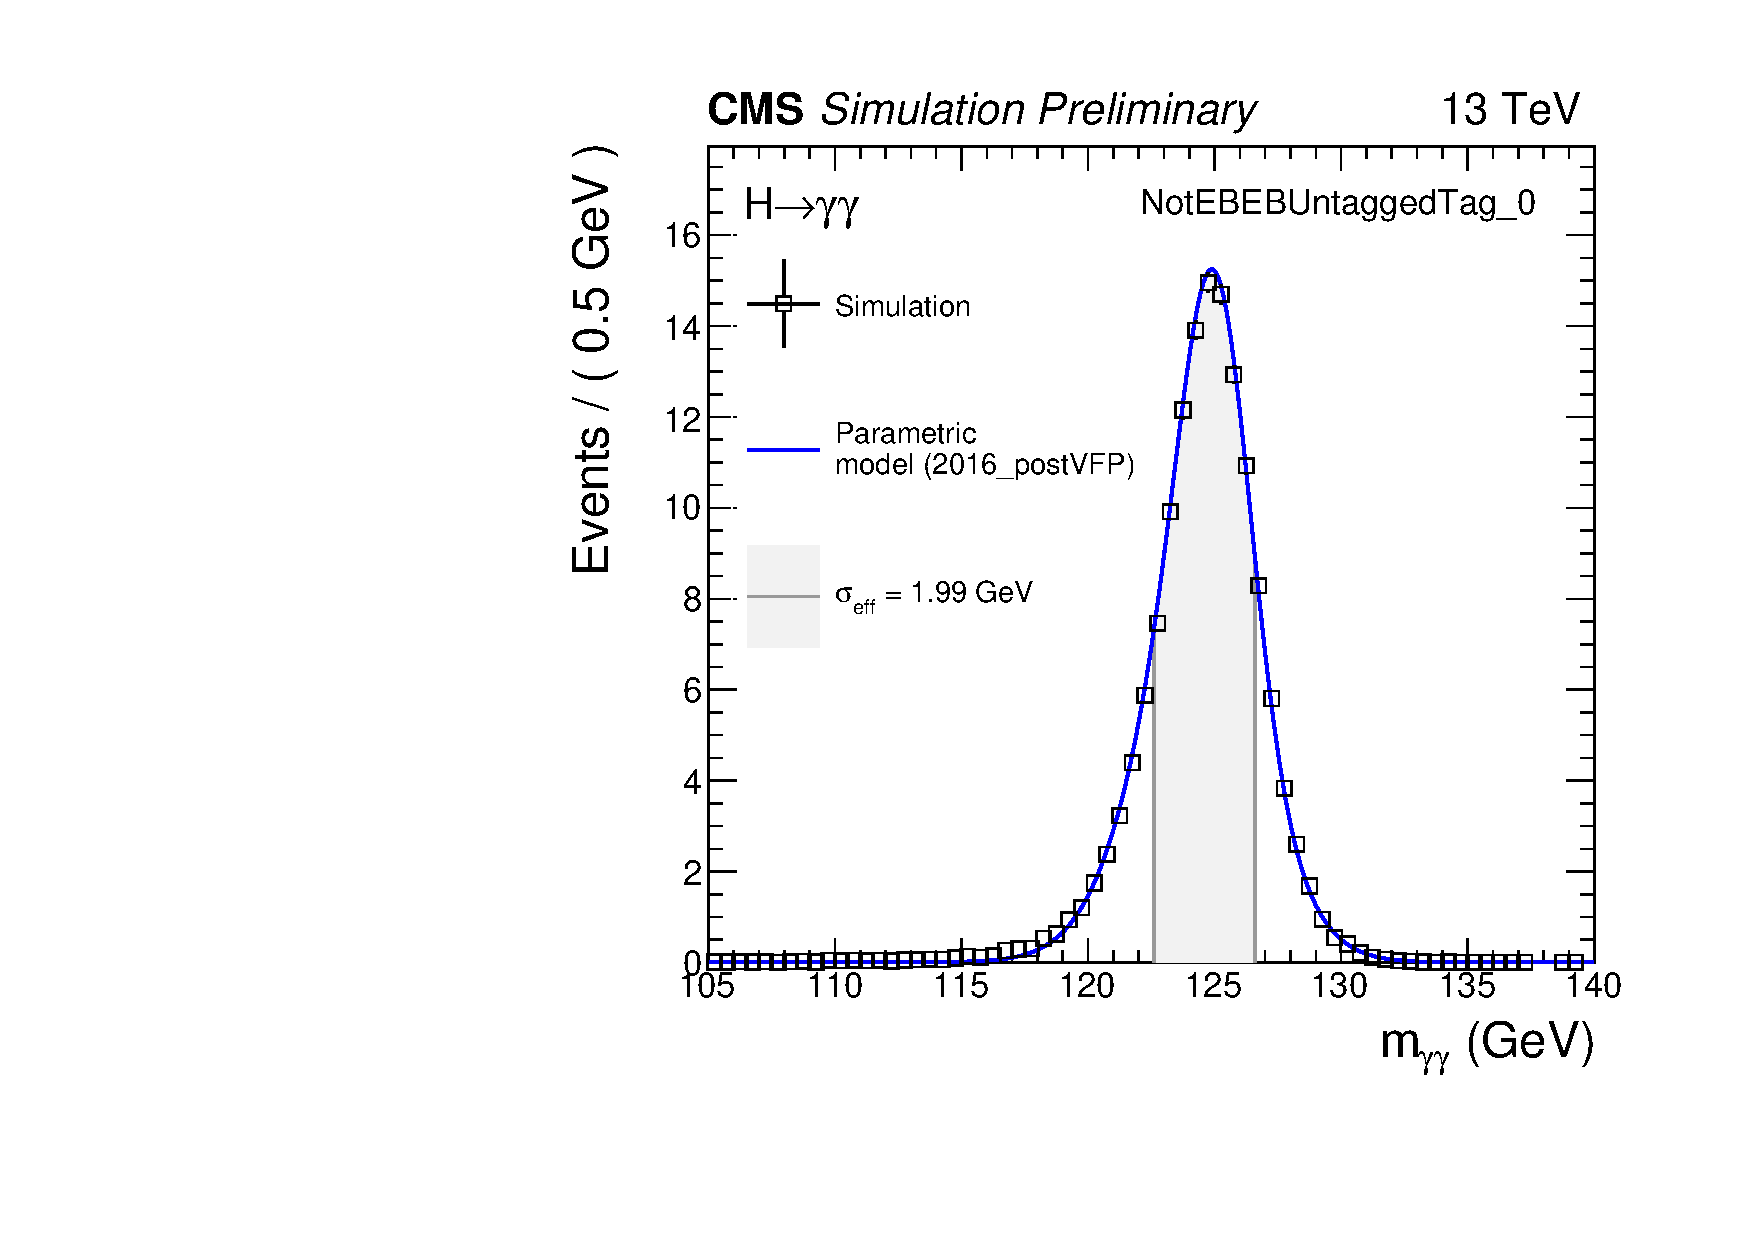
\includegraphics[width=\textwidth]{07-figures/signal_models/smodel_NotEBEBUntaggedTag_0_2016_postVFP.pdf}
            \end{center}
        \end{minipage}
    }~\subfloat{%
        \begin{minipage}[t]{0.5\textwidth}%
            \begin{center}
                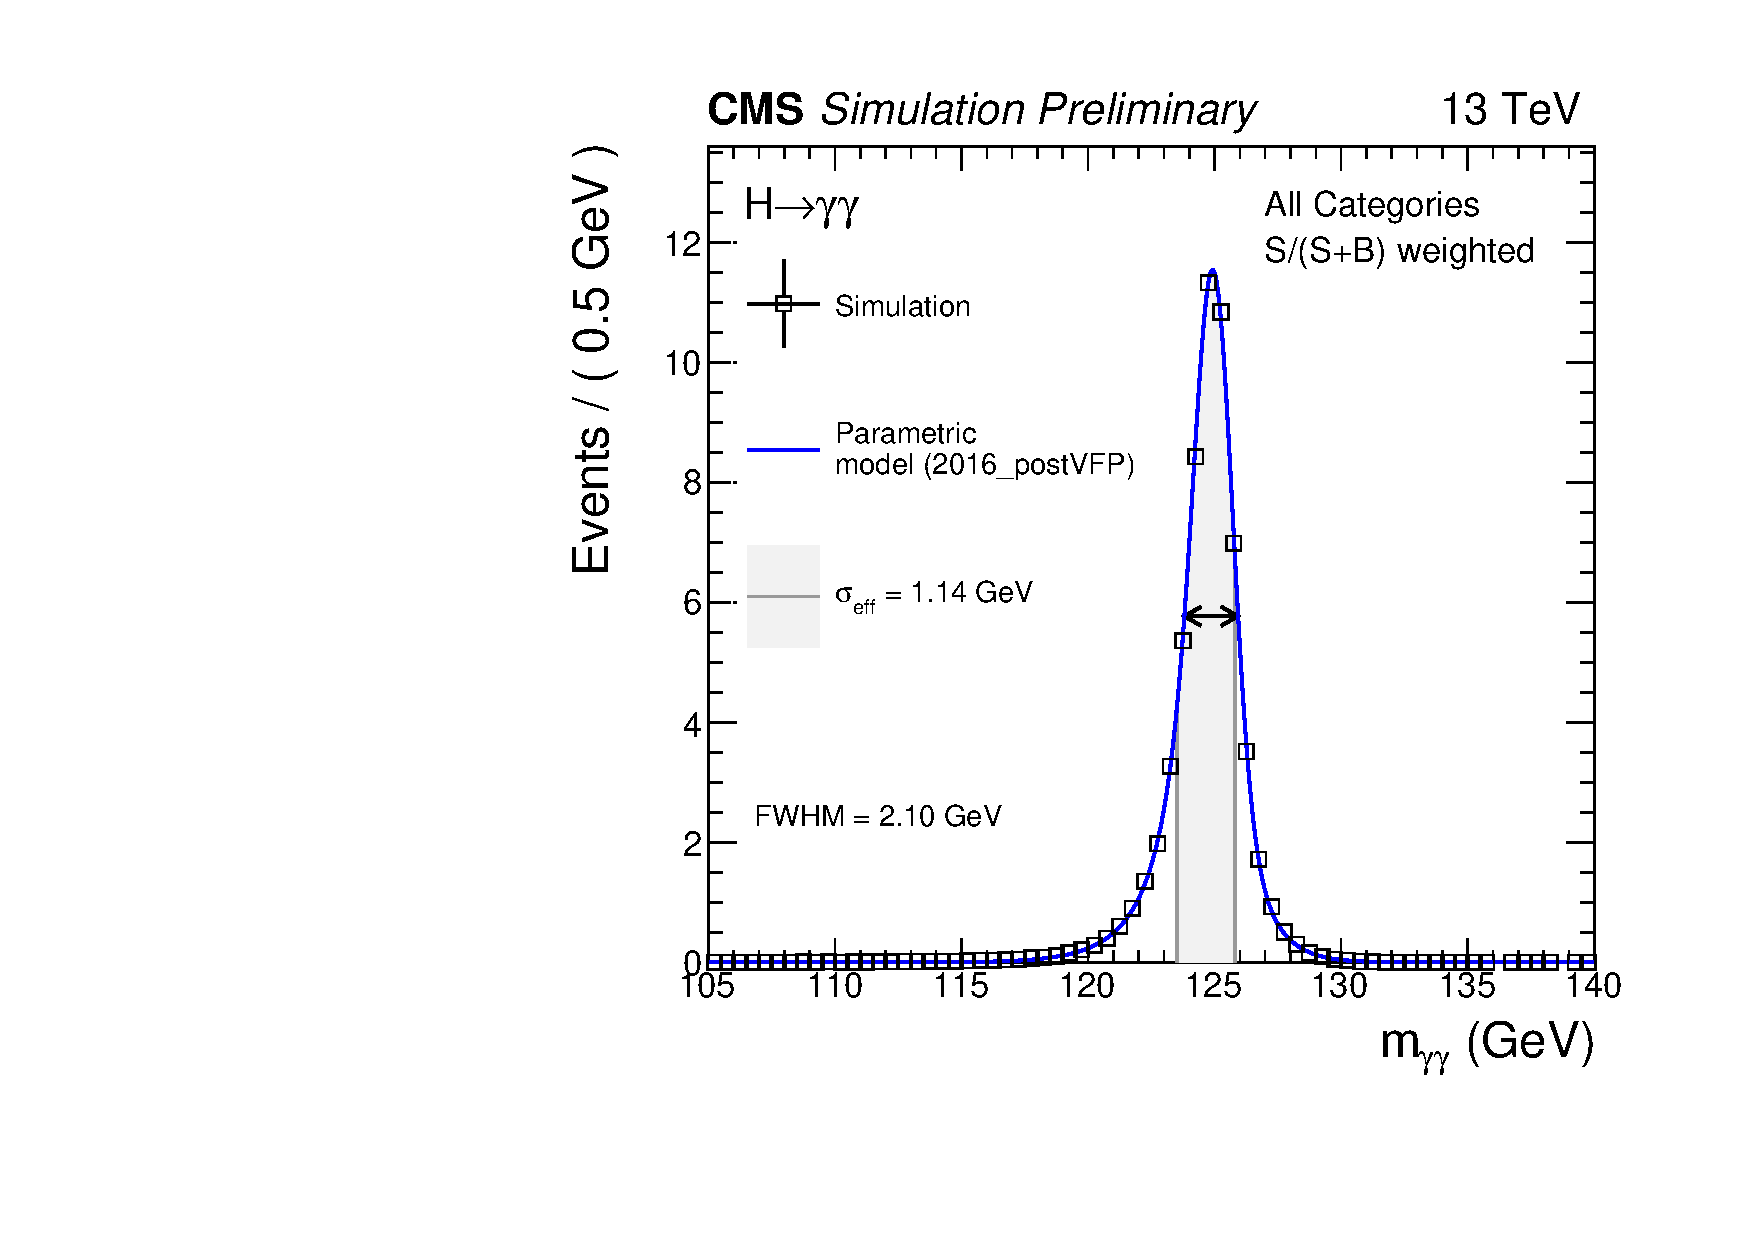
\includegraphics[width=\textwidth]{07-figures/signal_models/smodel_wall_2016_postVFP.pdf}
            \end{center}
        \end{minipage}
    }
    \caption[Signal models: 2016 postVFP]{Signal models for 2016 postVFP in each category and all categories combined.}
    \label{fig:signal_model_2016_postVFP}
\end{figure}

\begin{figure}[htbp!]
    \subfloat{%
        \begin{minipage}[t]{0.5\textwidth}%
            \begin{center}
                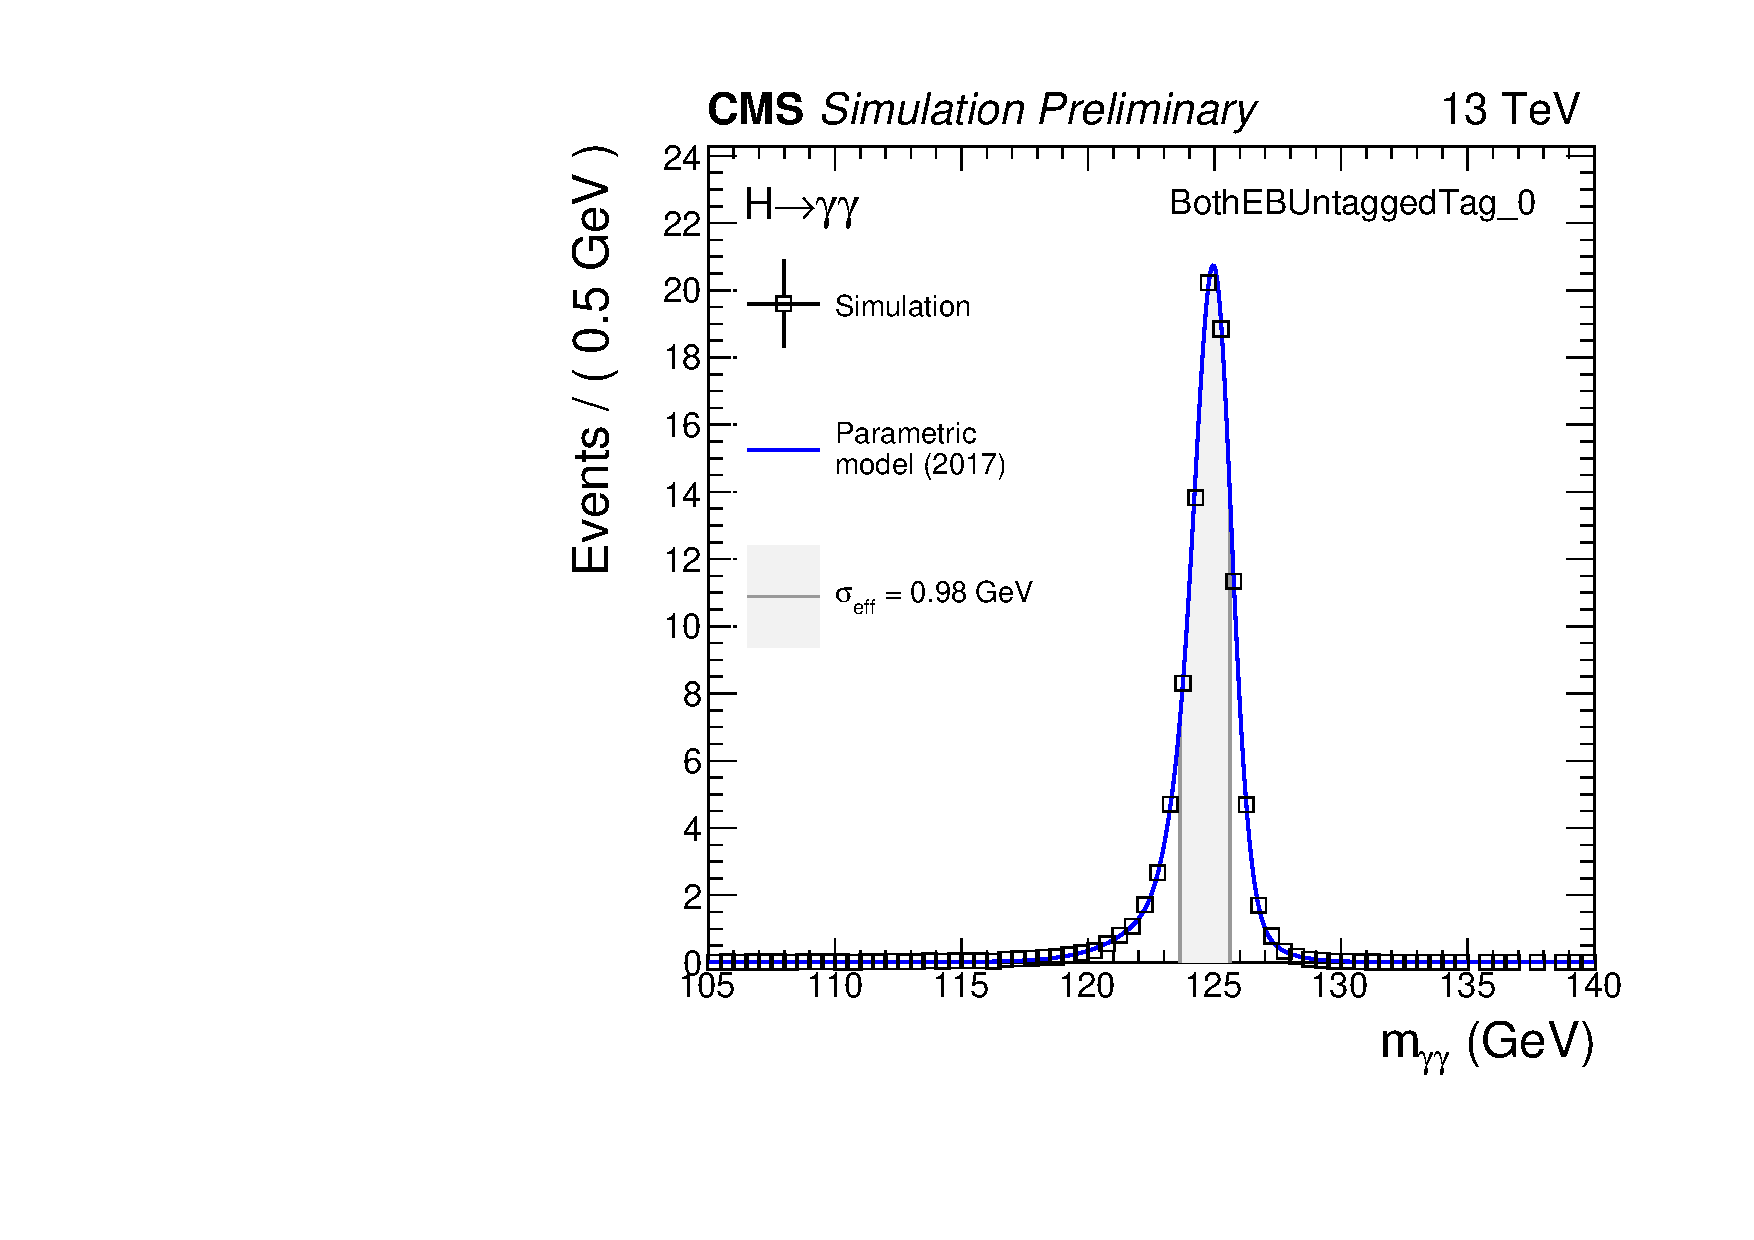
\includegraphics[width=\textwidth]{07-figures/signal_models/smodel_BothEBUntaggedTag_0_2017.pdf}
            \end{center}
        \end{minipage}
    }~\subfloat{%
        \begin{minipage}[t]{0.5\textwidth}%
            \begin{center}
                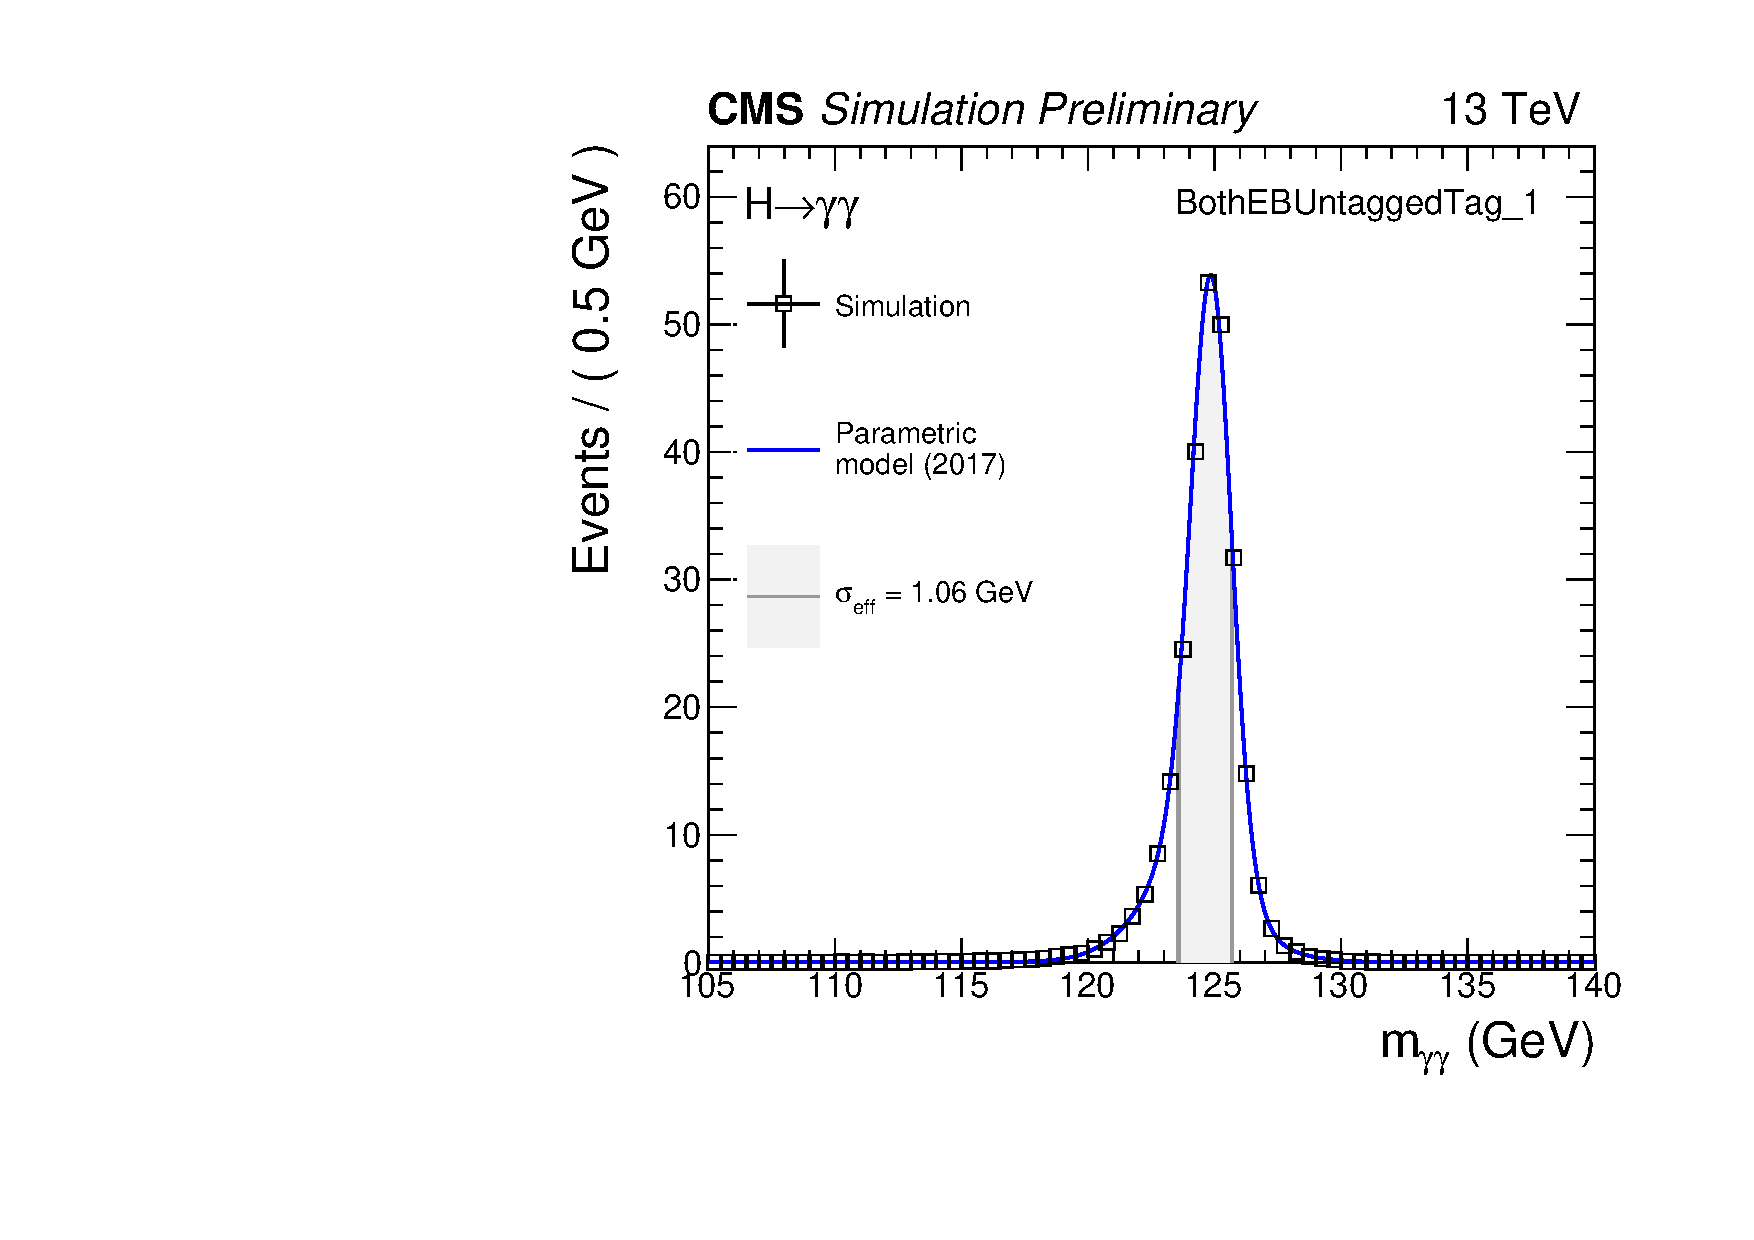
\includegraphics[width=\textwidth]{07-figures/signal_models/smodel_BothEBUntaggedTag_1_2017.pdf}
            \end{center}
        \end{minipage}
    }~\subfloat{%
        \begin{minipage}[t]{0.5\textwidth}%
            \begin{center}
                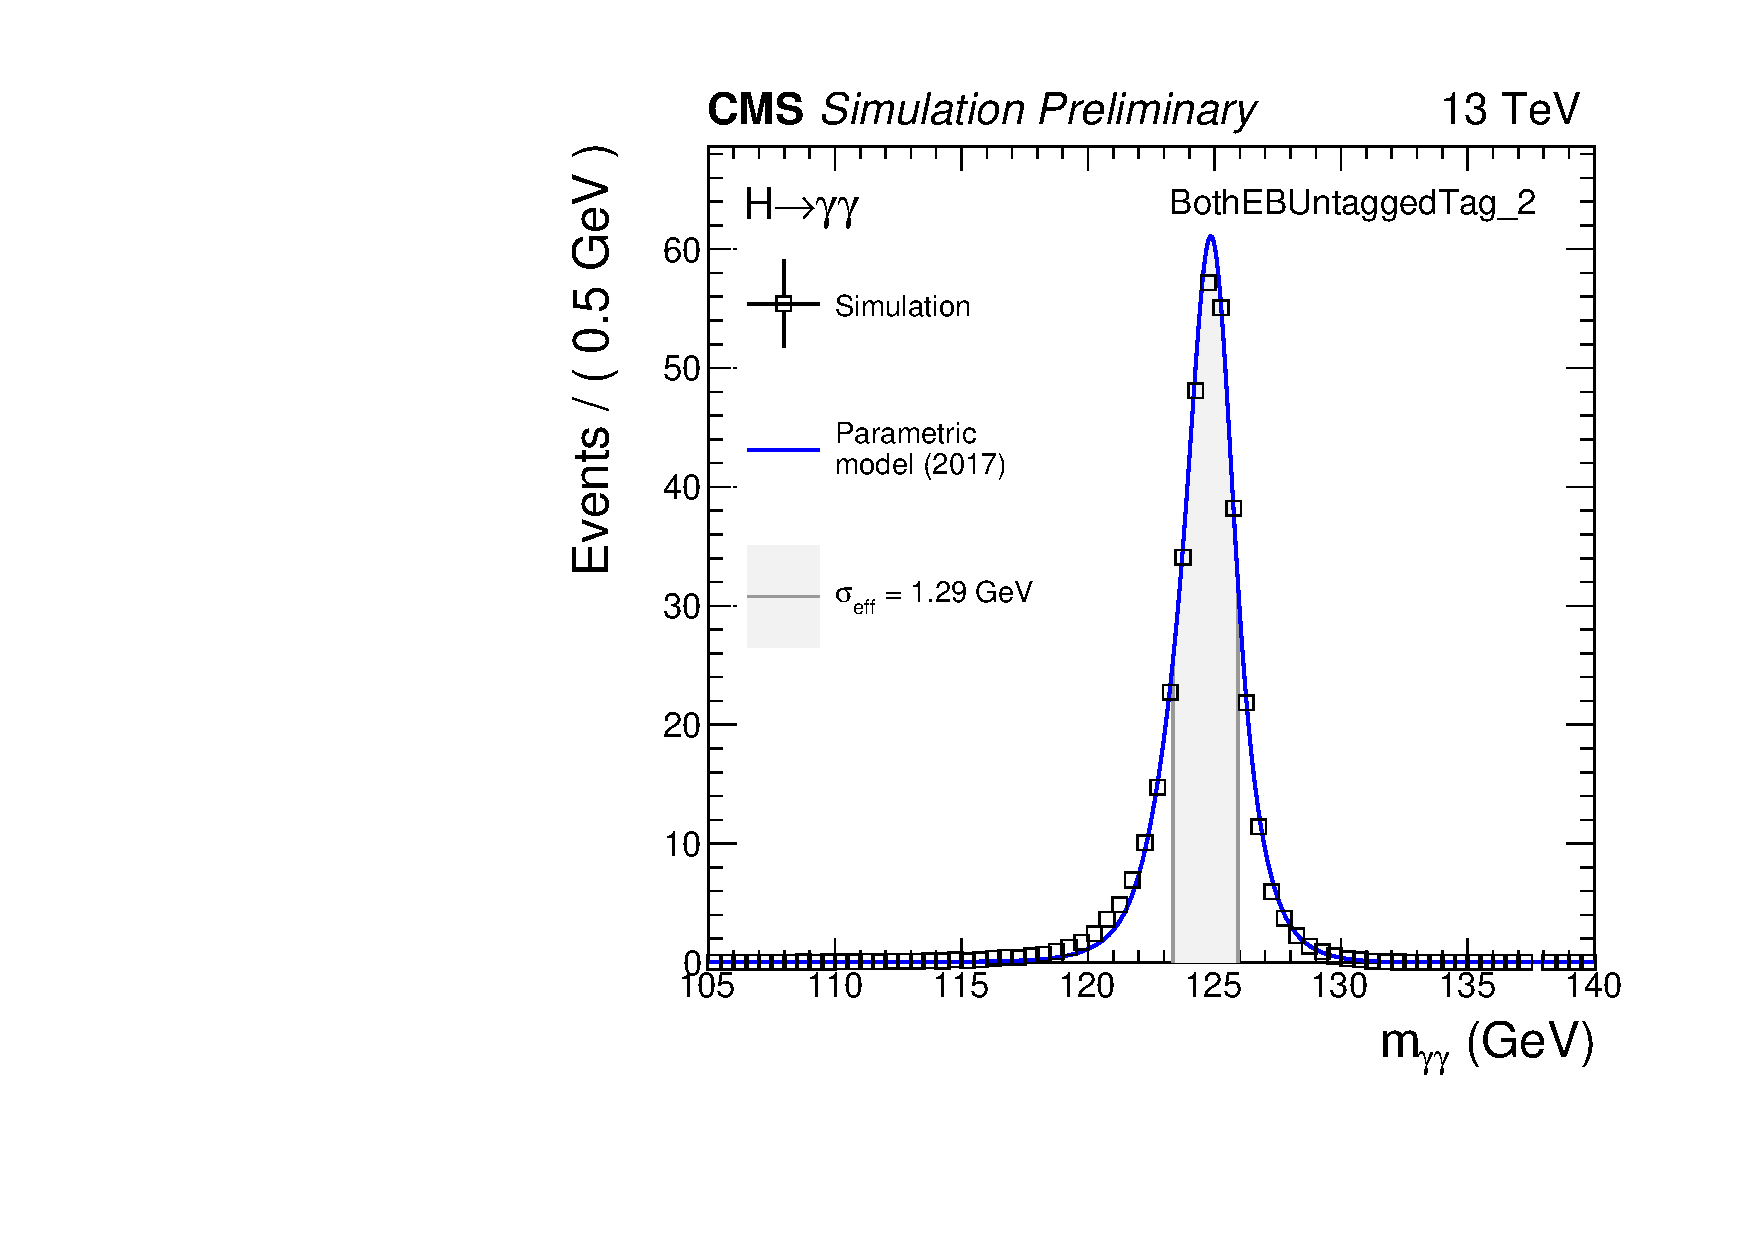
\includegraphics[width=\textwidth]{07-figures/signal_models/smodel_BothEBUntaggedTag_2_2017.pdf}
            \end{center}
        \end{minipage}
    }~\subfloat{%
        \begin{minipage}[t]{0.5\textwidth}%
            \begin{center}
                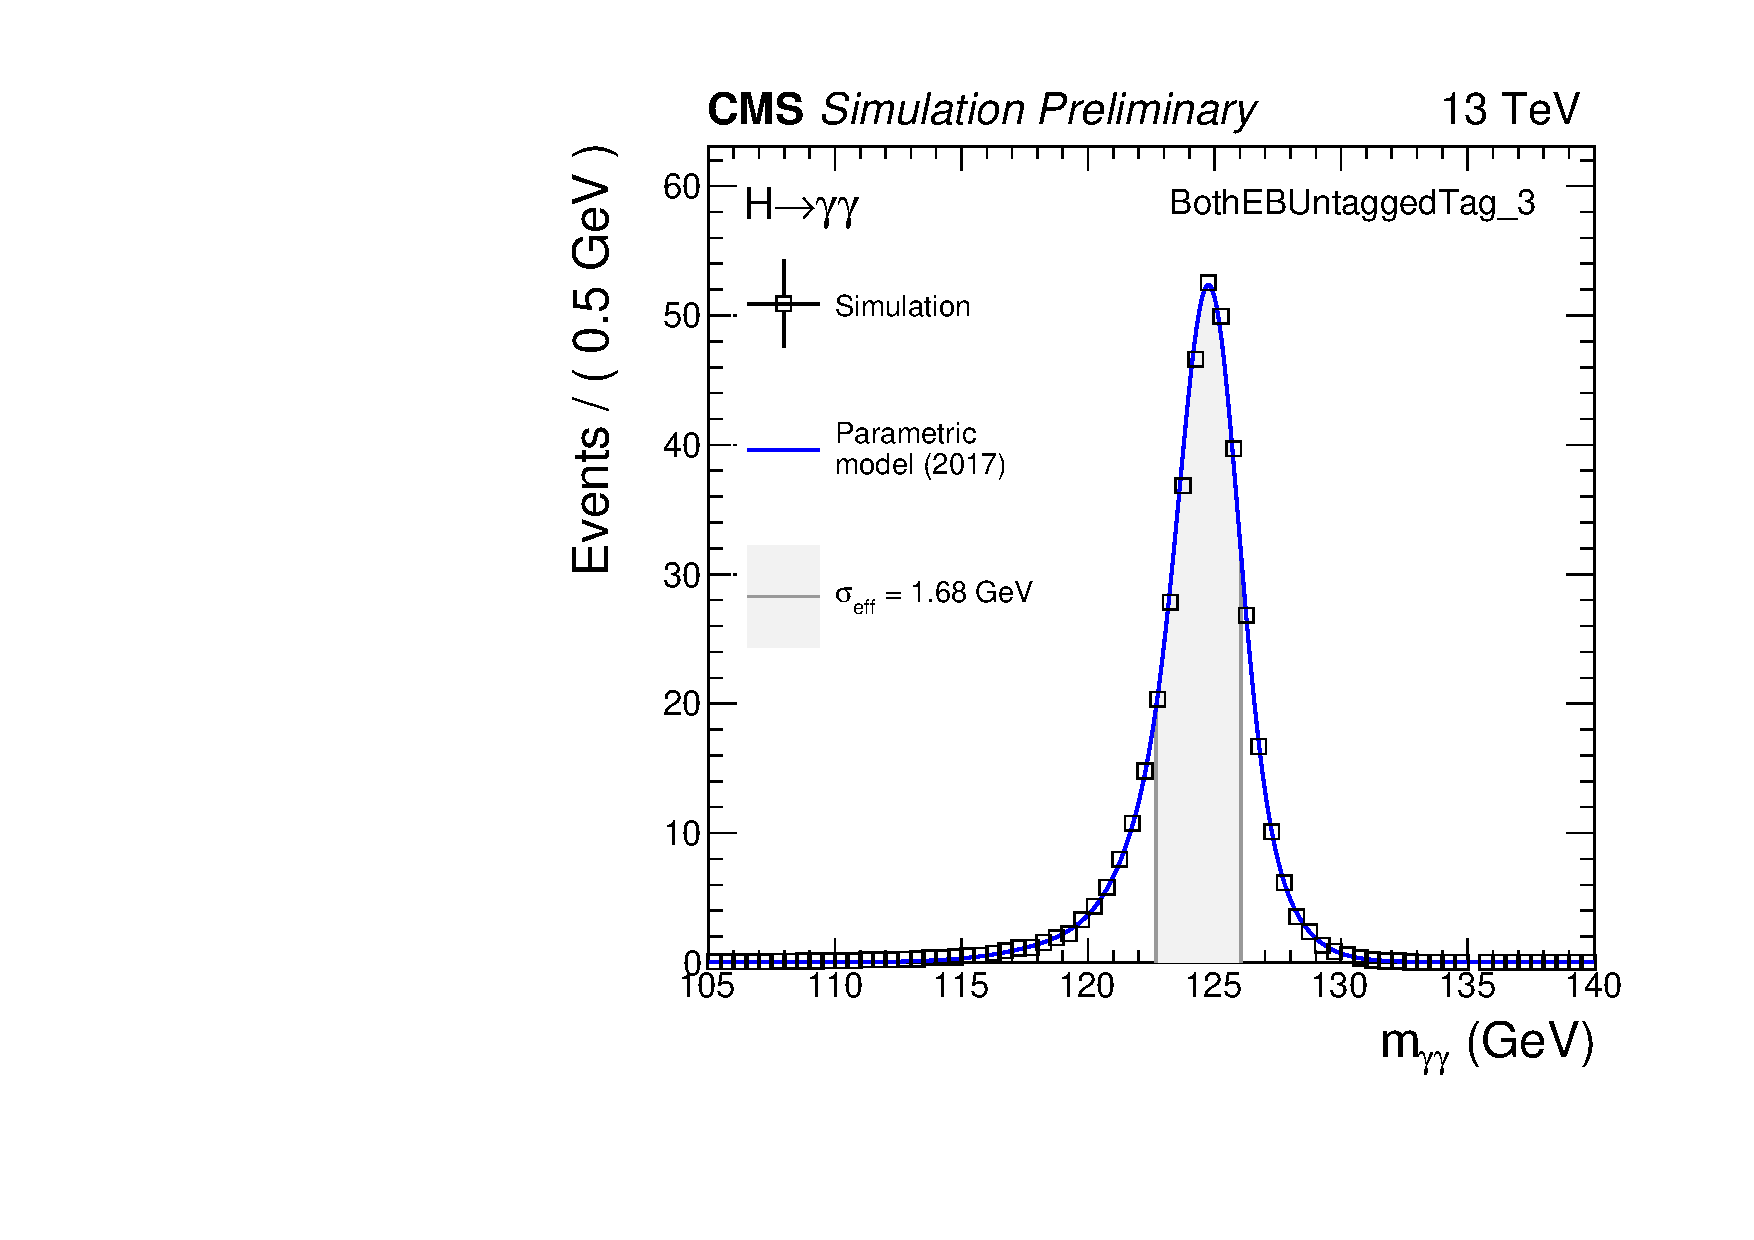
\includegraphics[width=\textwidth]{07-figures/signal_models/smodel_BothEBUntaggedTag_3_2017.pdf}
            \end{center}
        \end{minipage}
    }~\subfloat{%
        \begin{minipage}[t]{0.5\textwidth}%
            \begin{center}
                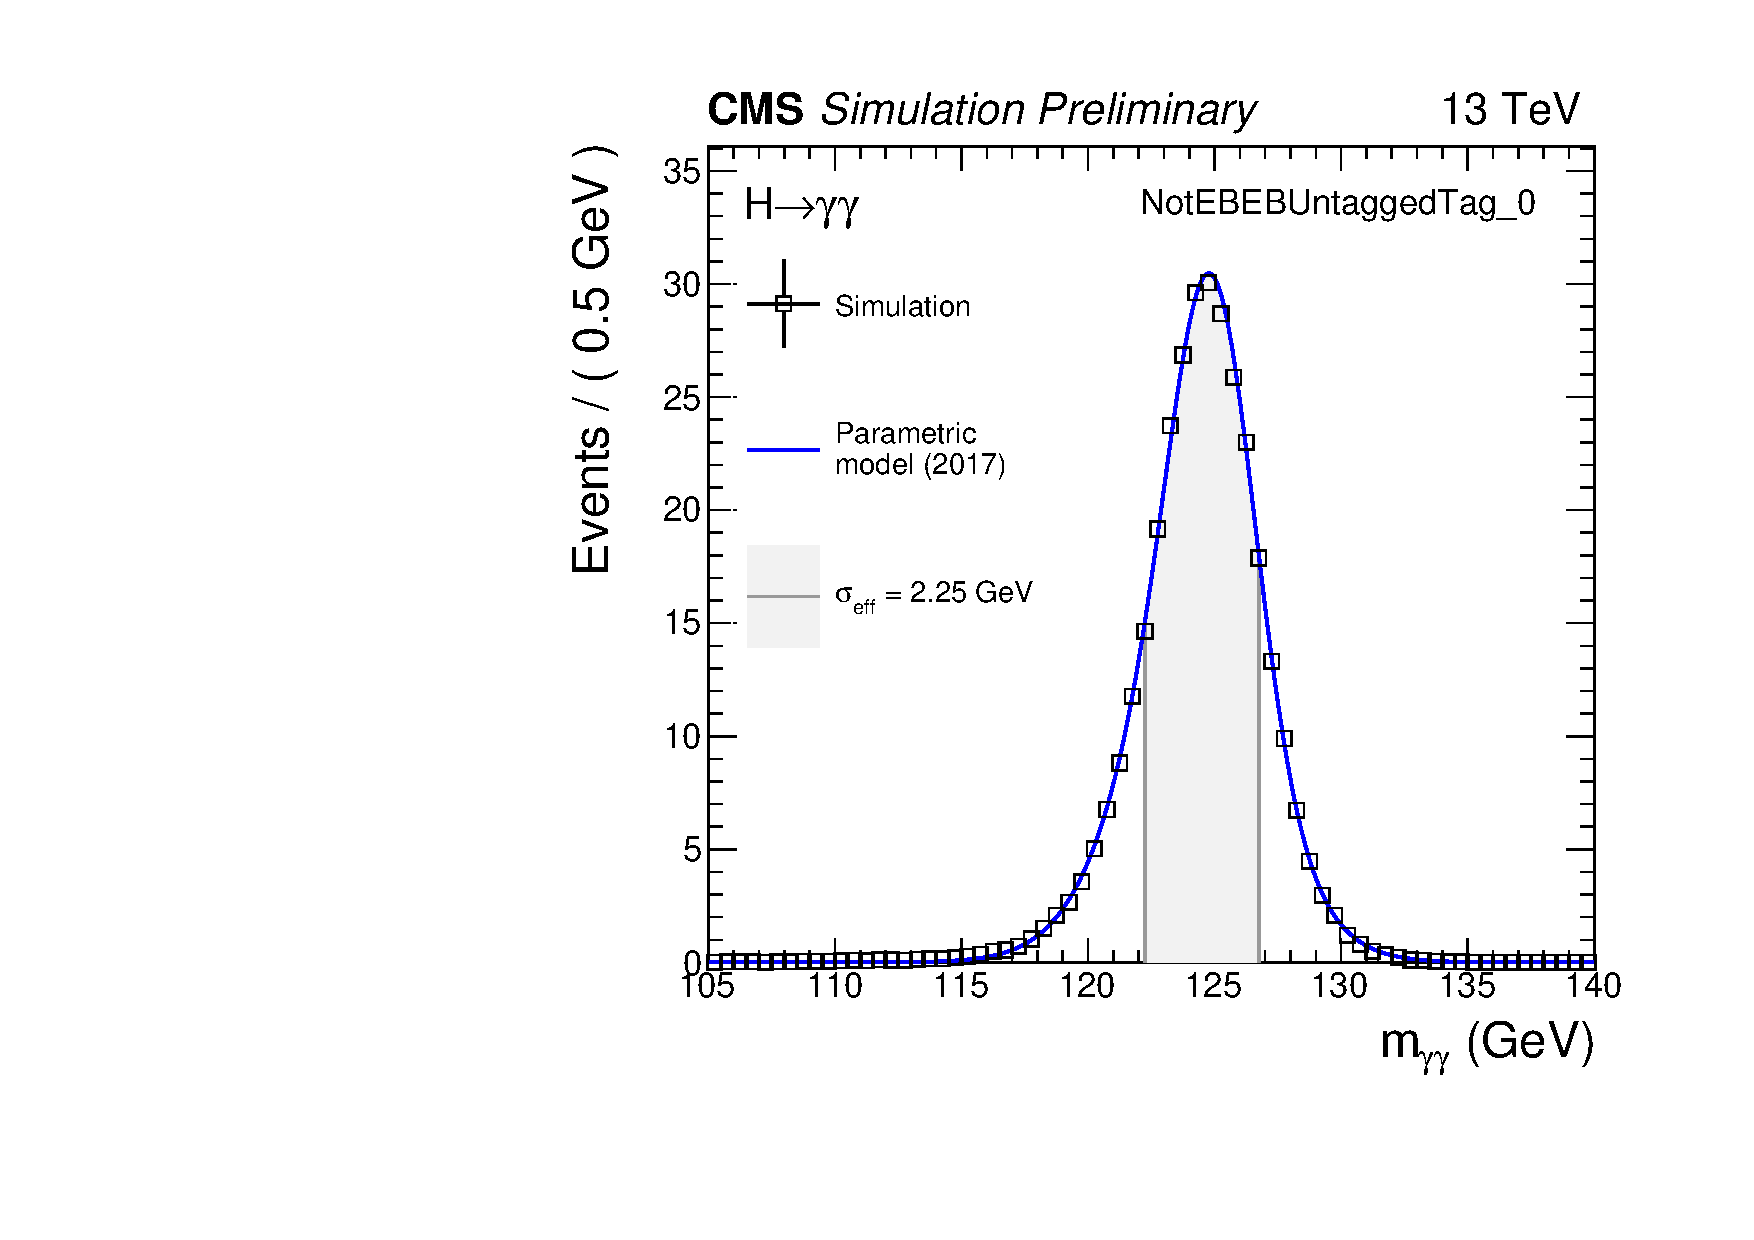
\includegraphics[width=\textwidth]{07-figures/signal_models/smodel_NotEBEBUntaggedTag_0_2017.pdf}
            \end{center}
        \end{minipage}
    }~\subfloat{%
        \begin{minipage}[t]{0.5\textwidth}%
            \begin{center}
                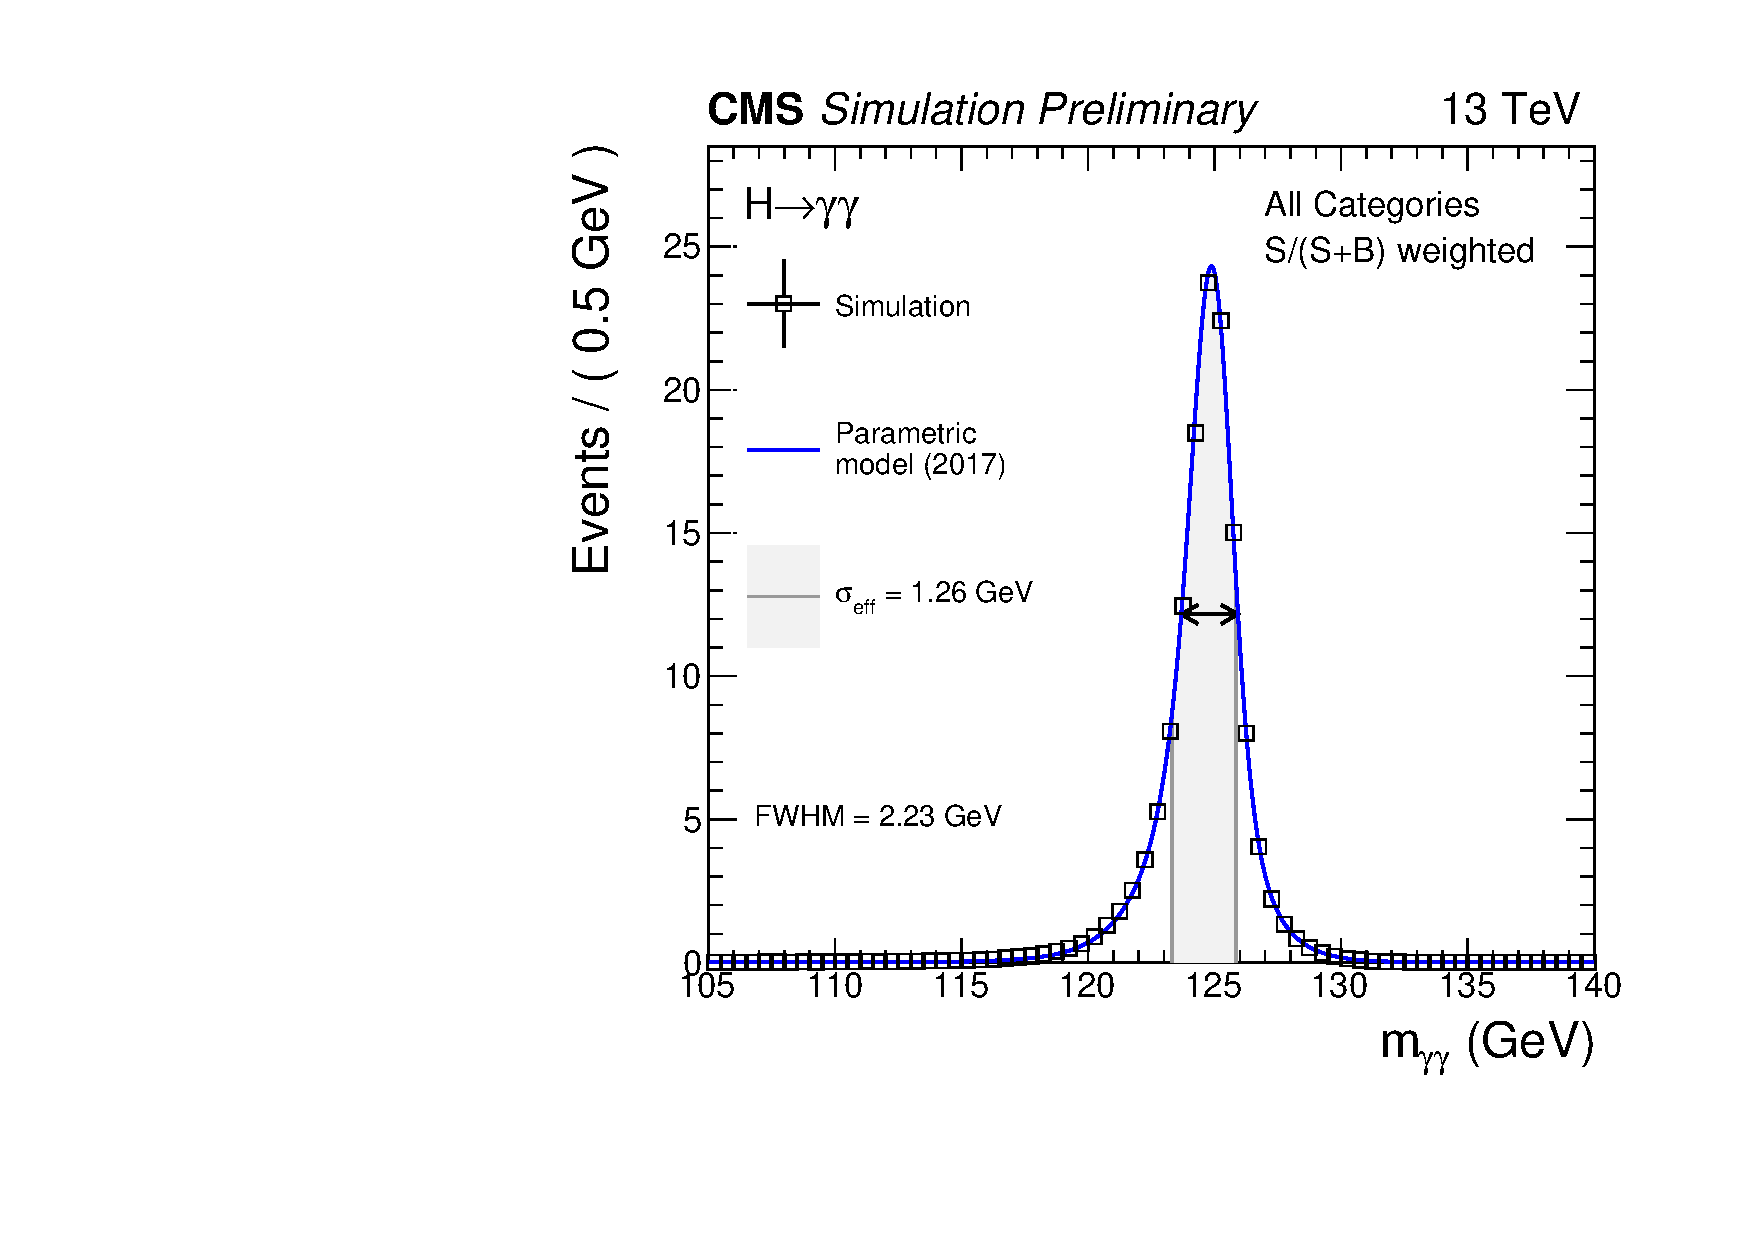
\includegraphics[width=\textwidth]{07-figures/signal_models/smodel_wall_2017.pdf}
            \end{center}
        \end{minipage}
    }
    \caption[Signal models: 2017]{Signal models for 2016 postVFP in each category and all categories combined.}
    \label{fig:signal_model_2017}
\end{figure}

\begin{figure}[htbp!]
    \subfloat{%
        \begin{minipage}[t]{0.5\textwidth}%
            \begin{center}
                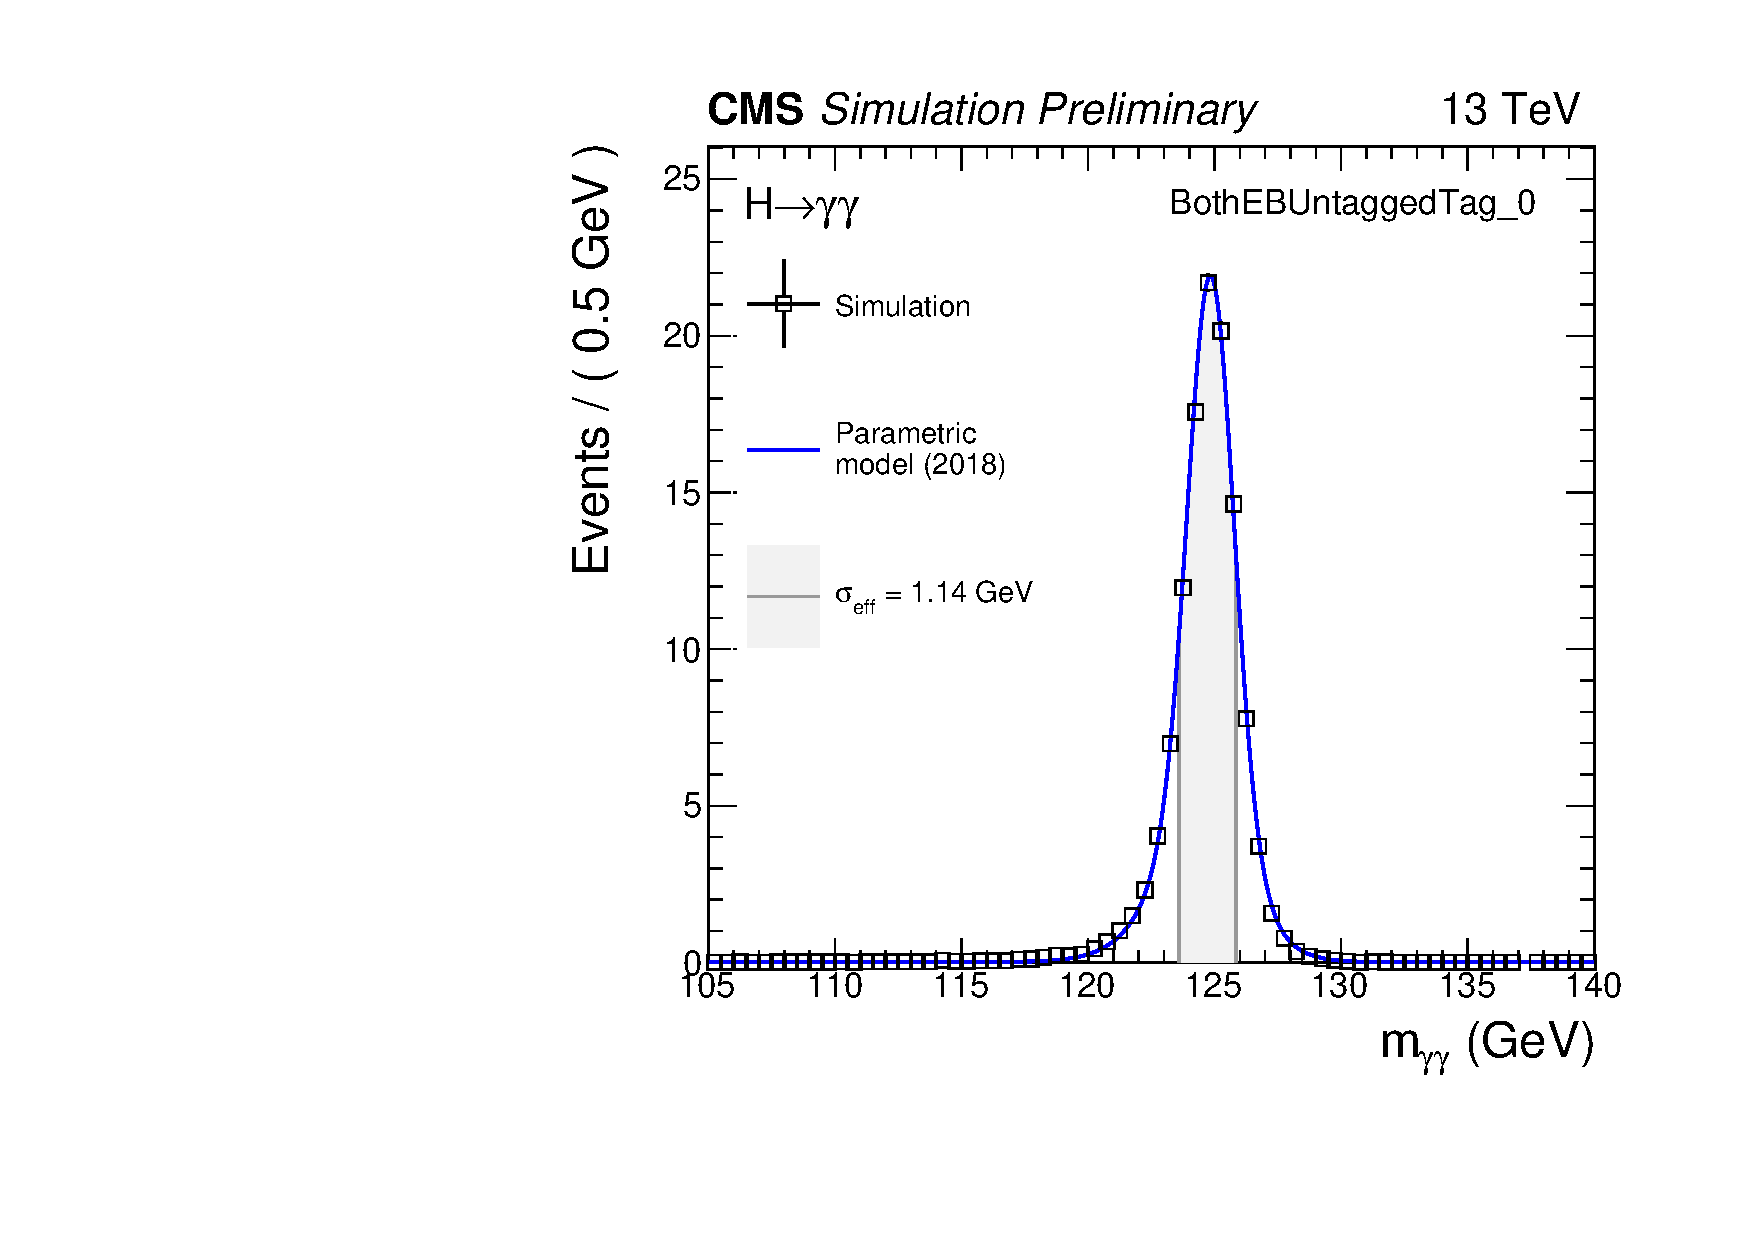
\includegraphics[width=\textwidth]{07-figures/signal_models/smodel_BothEBUntaggedTag_0_2018.pdf}
            \end{center}
        \end{minipage}
    }~\subfloat{%
        \begin{minipage}[t]{0.5\textwidth}%
            \begin{center}
                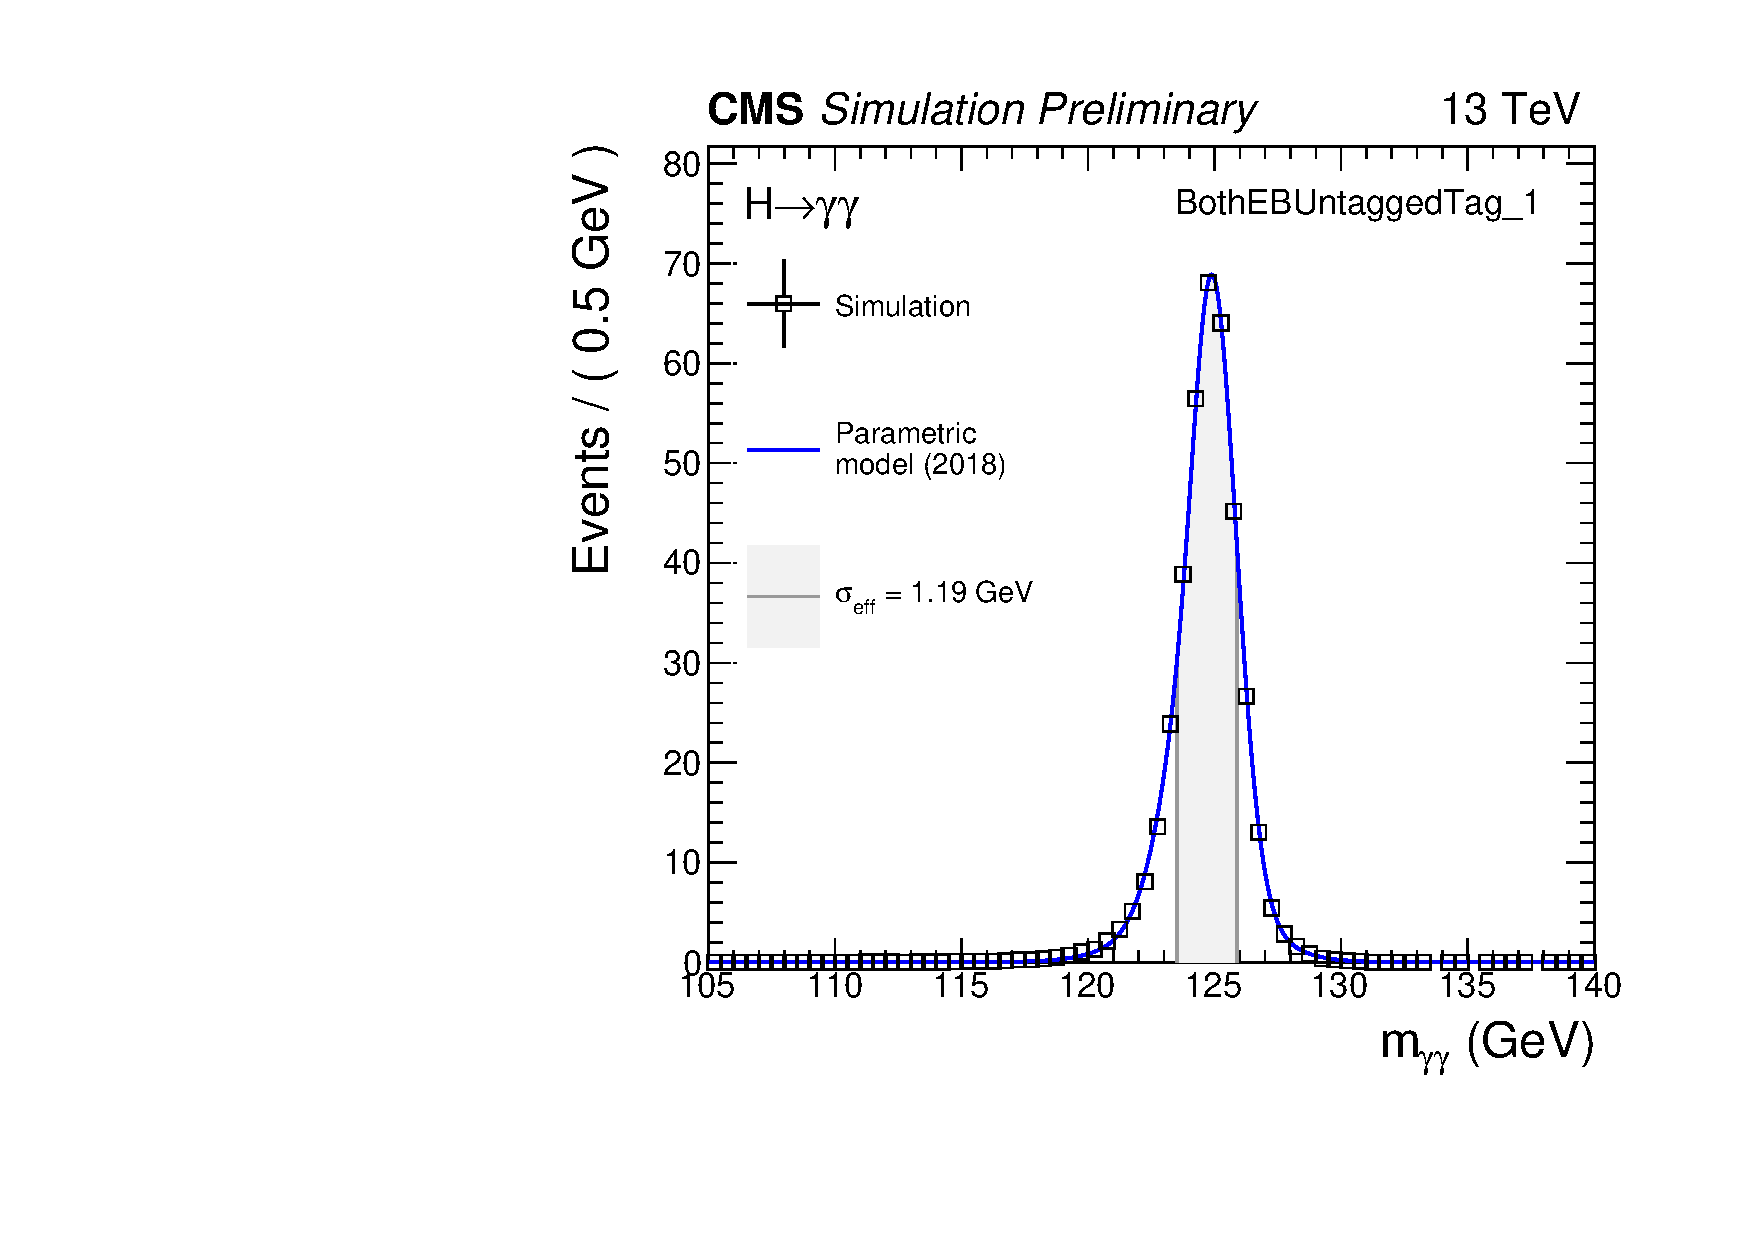
\includegraphics[width=\textwidth]{07-figures/signal_models/smodel_BothEBUntaggedTag_1_2018.pdf}
            \end{center}
        \end{minipage}
    }~\subfloat{%
        \begin{minipage}[t]{0.5\textwidth}%
            \begin{center}
                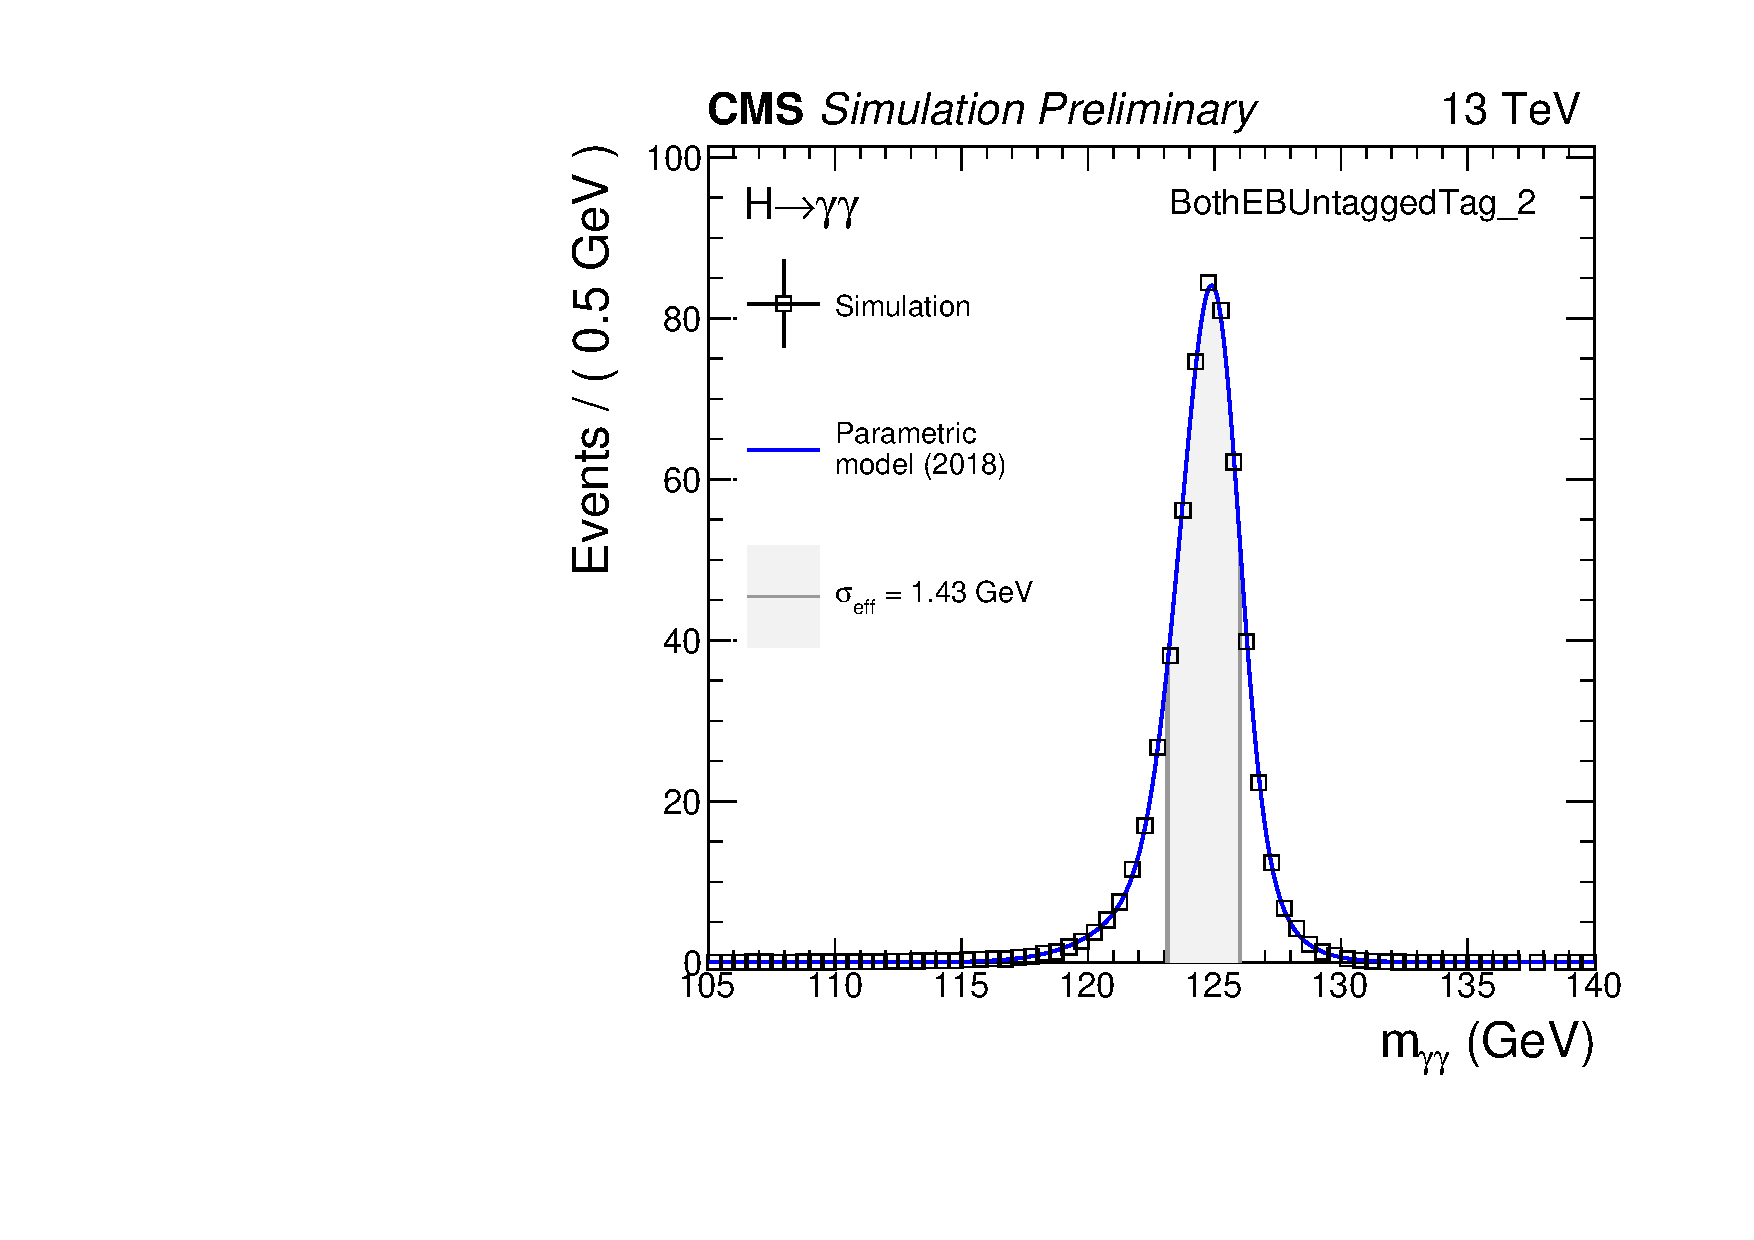
\includegraphics[width=\textwidth]{07-figures/signal_models/smodel_BothEBUntaggedTag_2_2018.pdf}
            \end{center}
        \end{minipage}
    }~\subfloat{%
        \begin{minipage}[t]{0.5\textwidth}%
            \begin{center}
                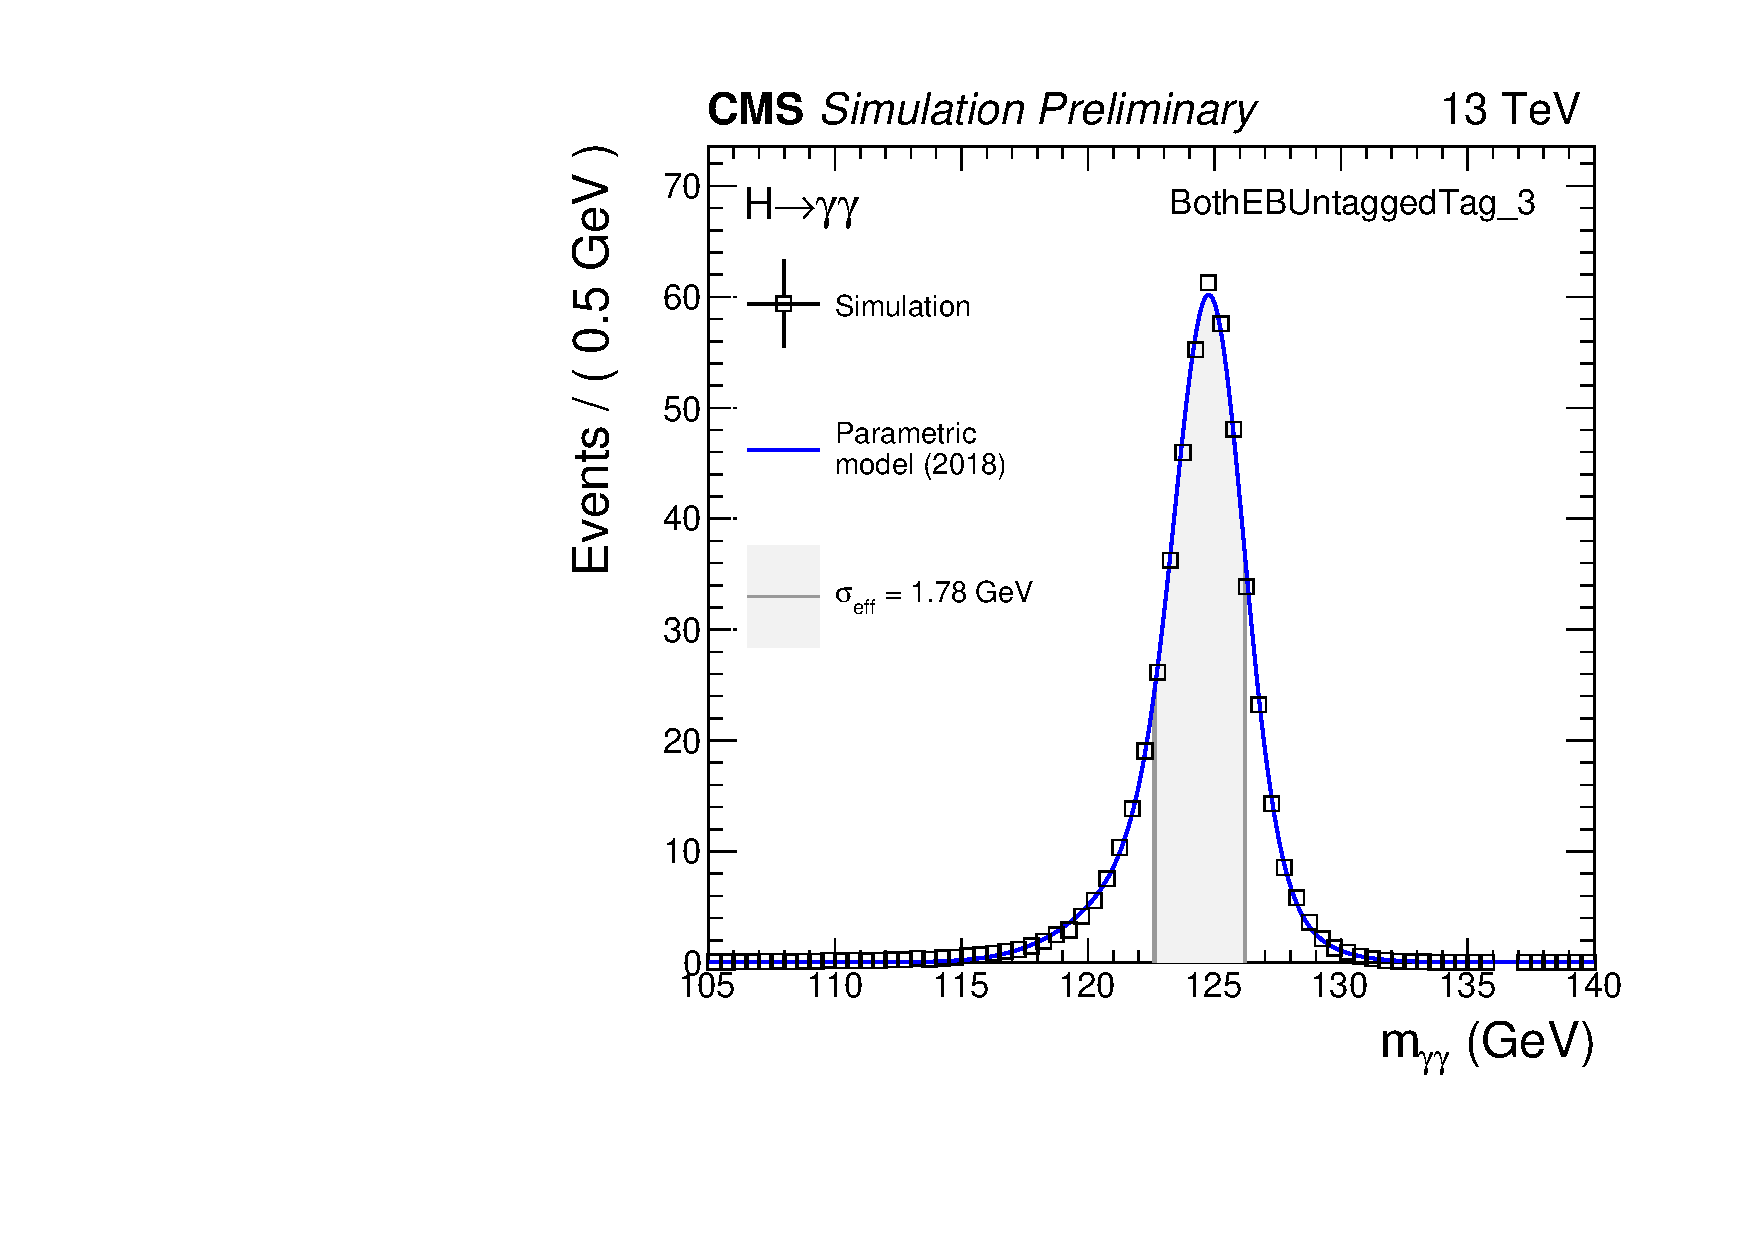
\includegraphics[width=\textwidth]{07-figures/signal_models/smodel_BothEBUntaggedTag_3_2018.pdf}
            \end{center}
        \end{minipage}
    }~\subfloat{%
        \begin{minipage}[t]{0.5\textwidth}%
            \begin{center}
                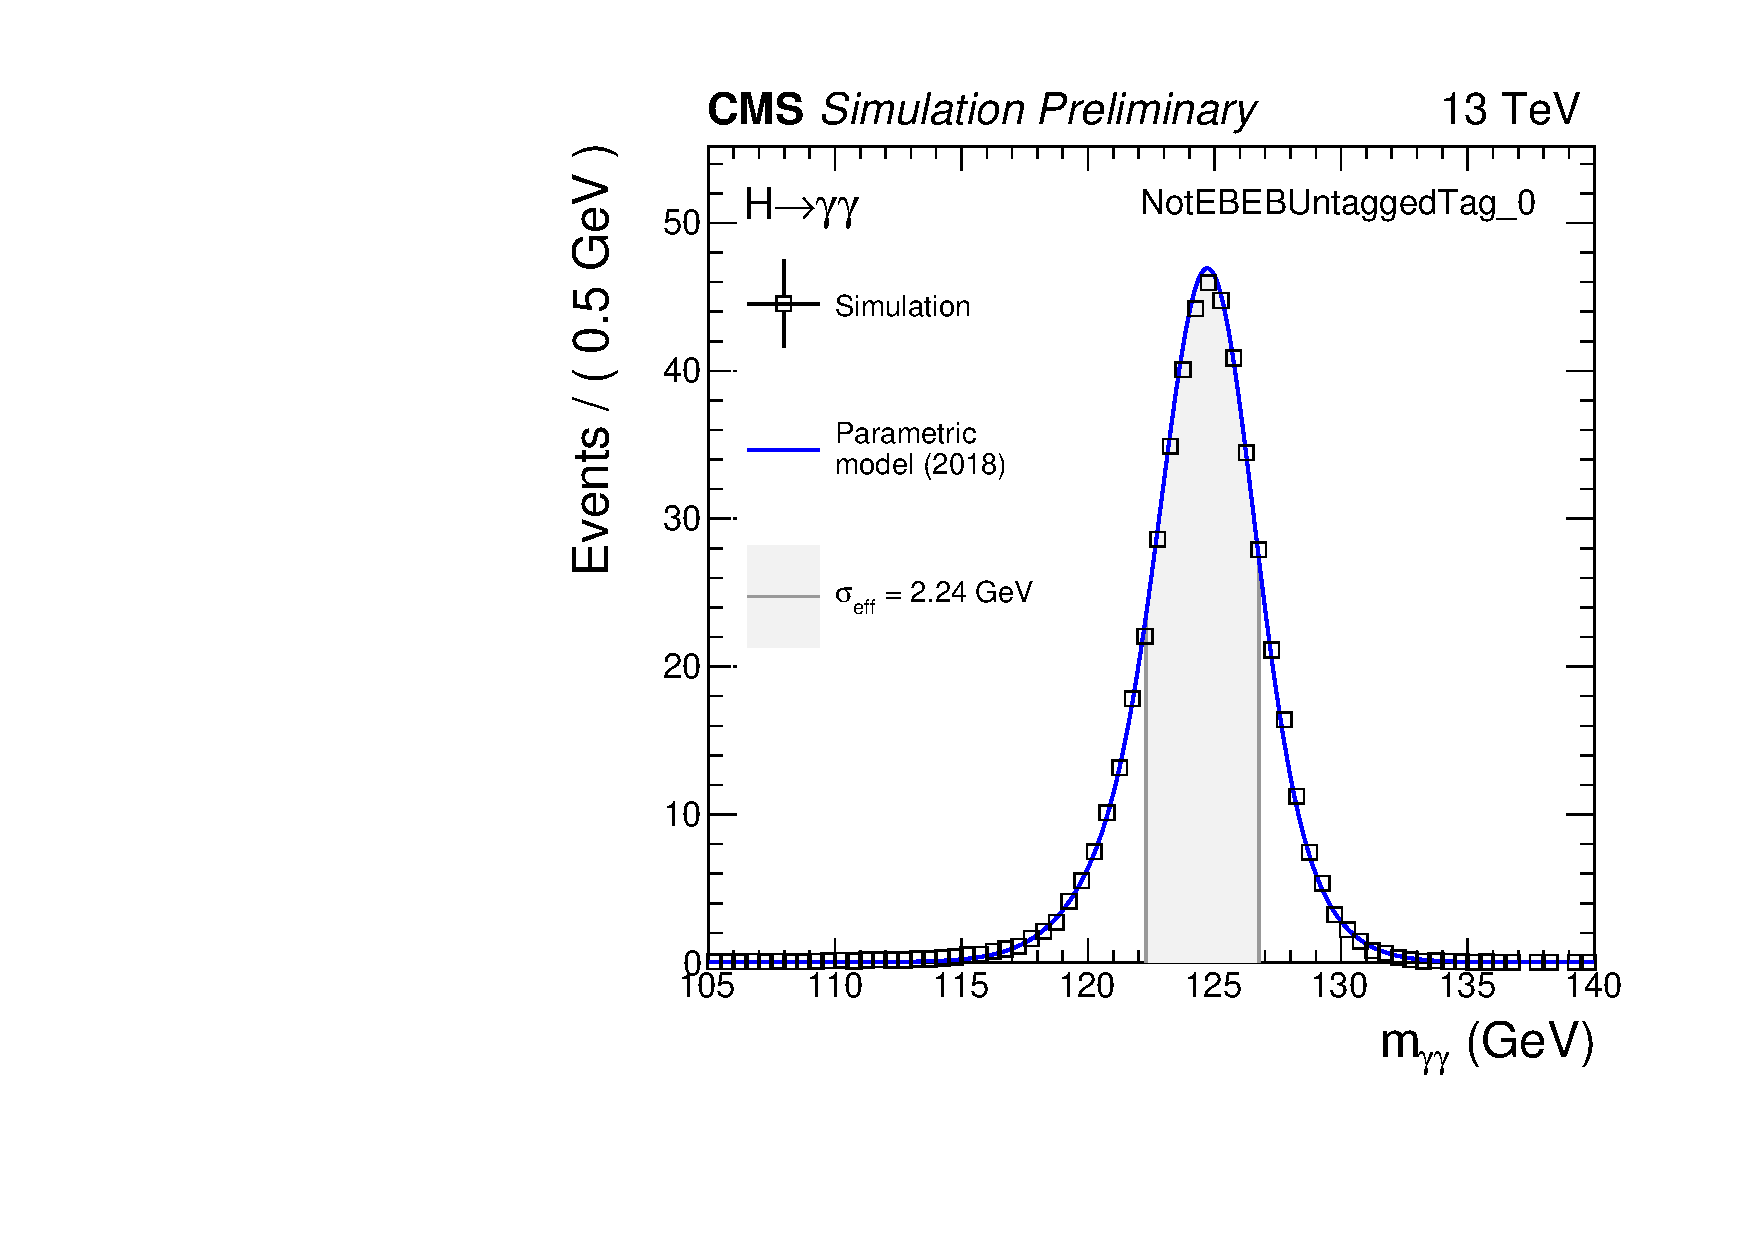
\includegraphics[width=\textwidth]{07-figures/signal_models/smodel_NotEBEBUntaggedTag_0_2018.pdf}
            \end{center}
        \end{minipage}
    }~\subfloat{%
        \begin{minipage}[t]{0.5\textwidth}%
            \begin{center}
                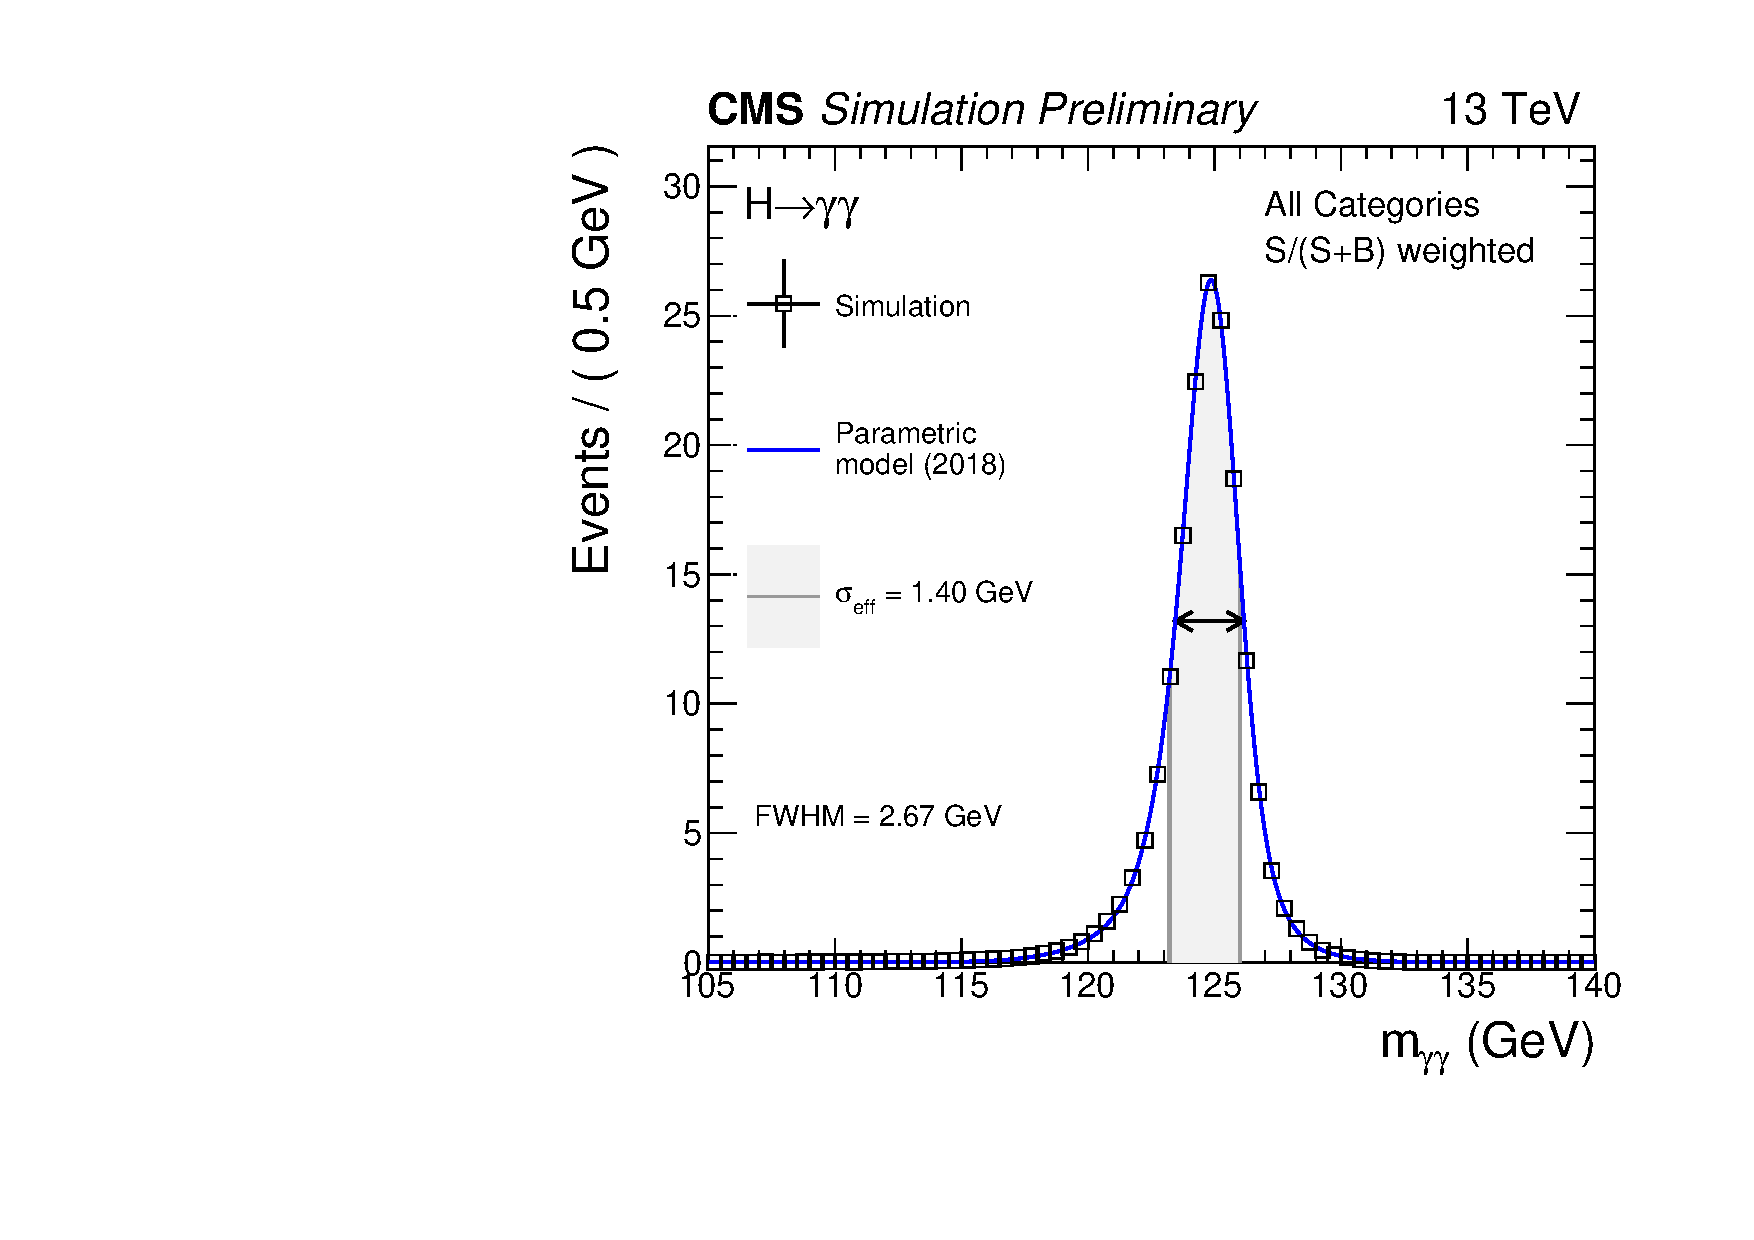
\includegraphics[width=\textwidth]{07-figures/signal_models/smodel_wall_2018.pdf}
            \end{center}
        \end{minipage}
    }
    \caption[Signal models: 2018]{Signal models for 2018 in each category and all categories combined.}
    \label{fig:signal_model_2018}
\end{figure}



\begin{figure}[htbp!]
    \subfloat{%
        \begin{minipage}[t]{0.5\textwidth}%
            \begin{center}
                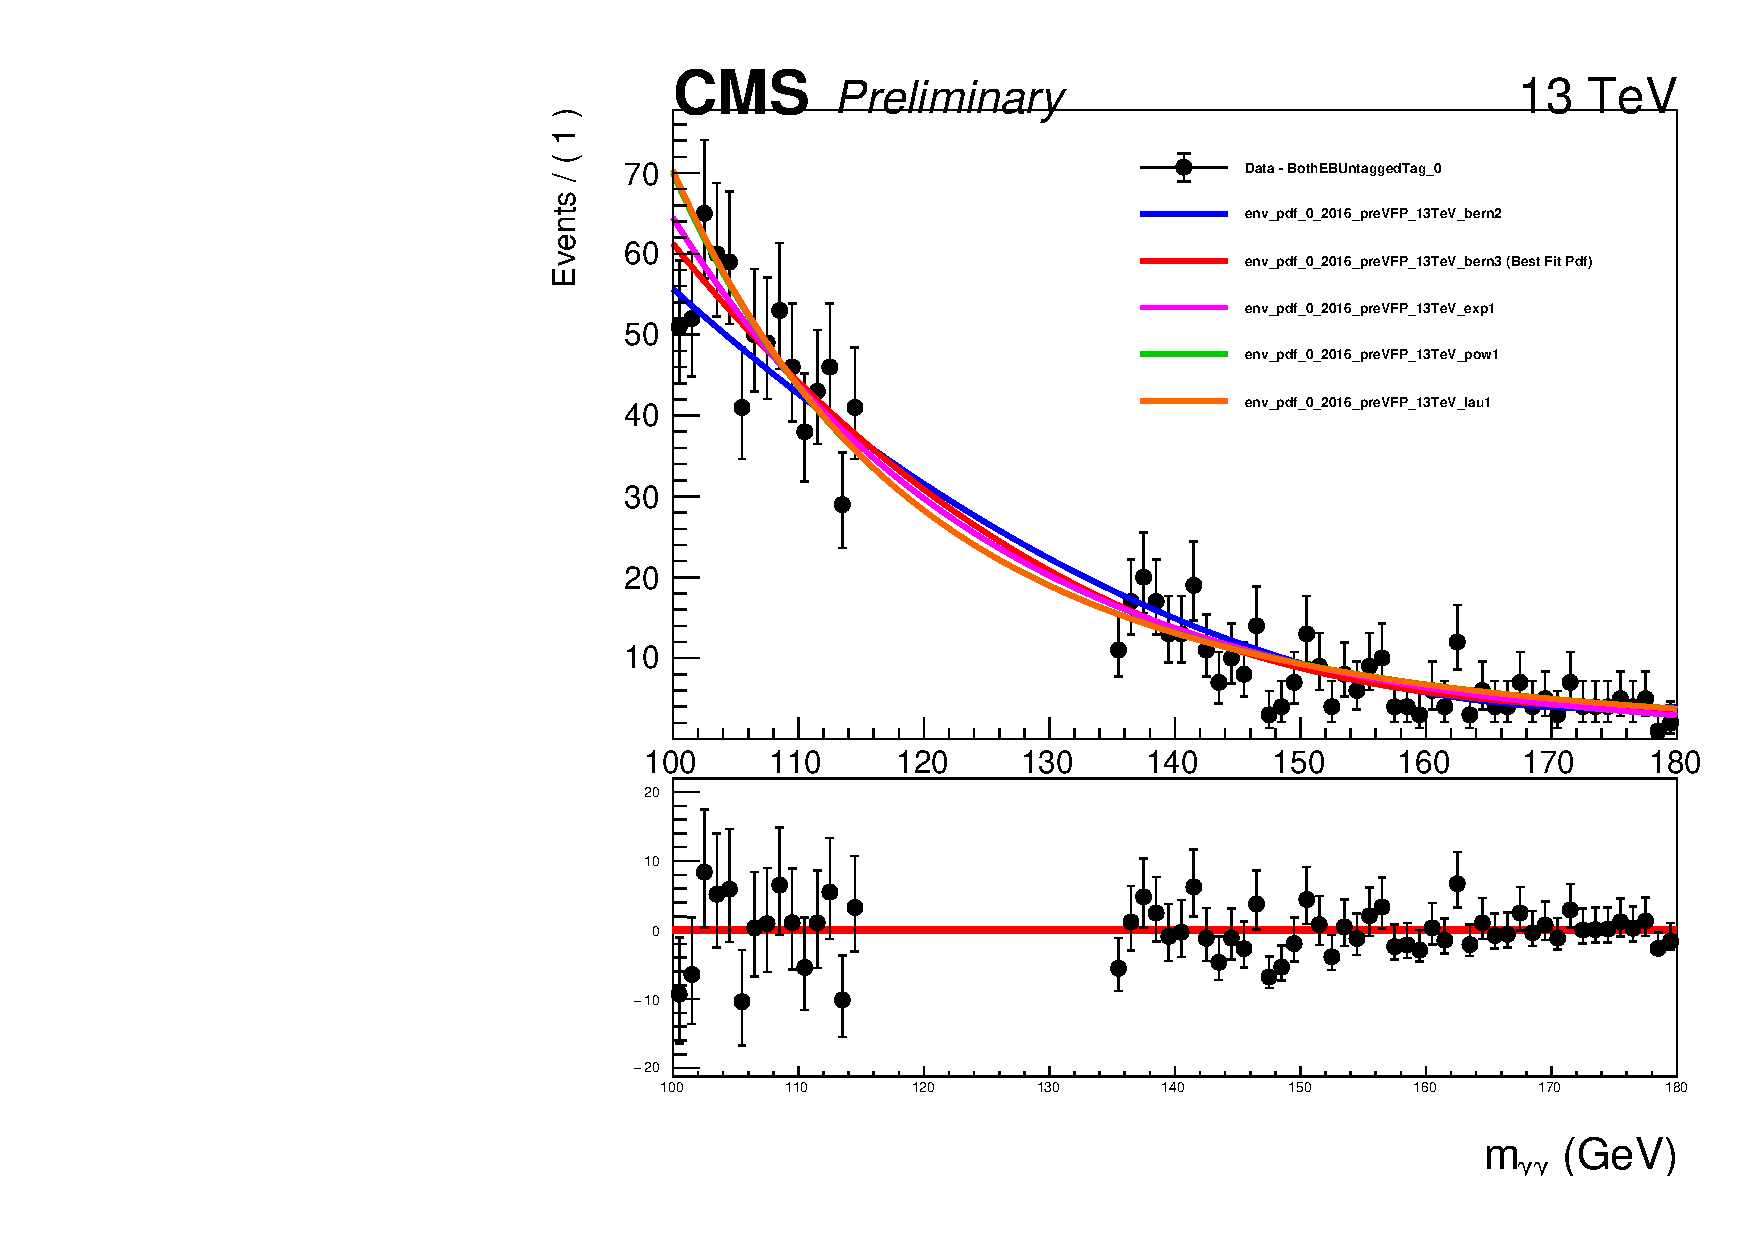
\includegraphics[width=0.925\textwidth]{07-figures/bkg_models/multipdf_BothEBUntaggedTag_0_2016preVFP.pdf}
            \end{center}
        \end{minipage}
    }~\subfloat{%
        \begin{minipage}[t]{0.5\textwidth}%
            \begin{center}
                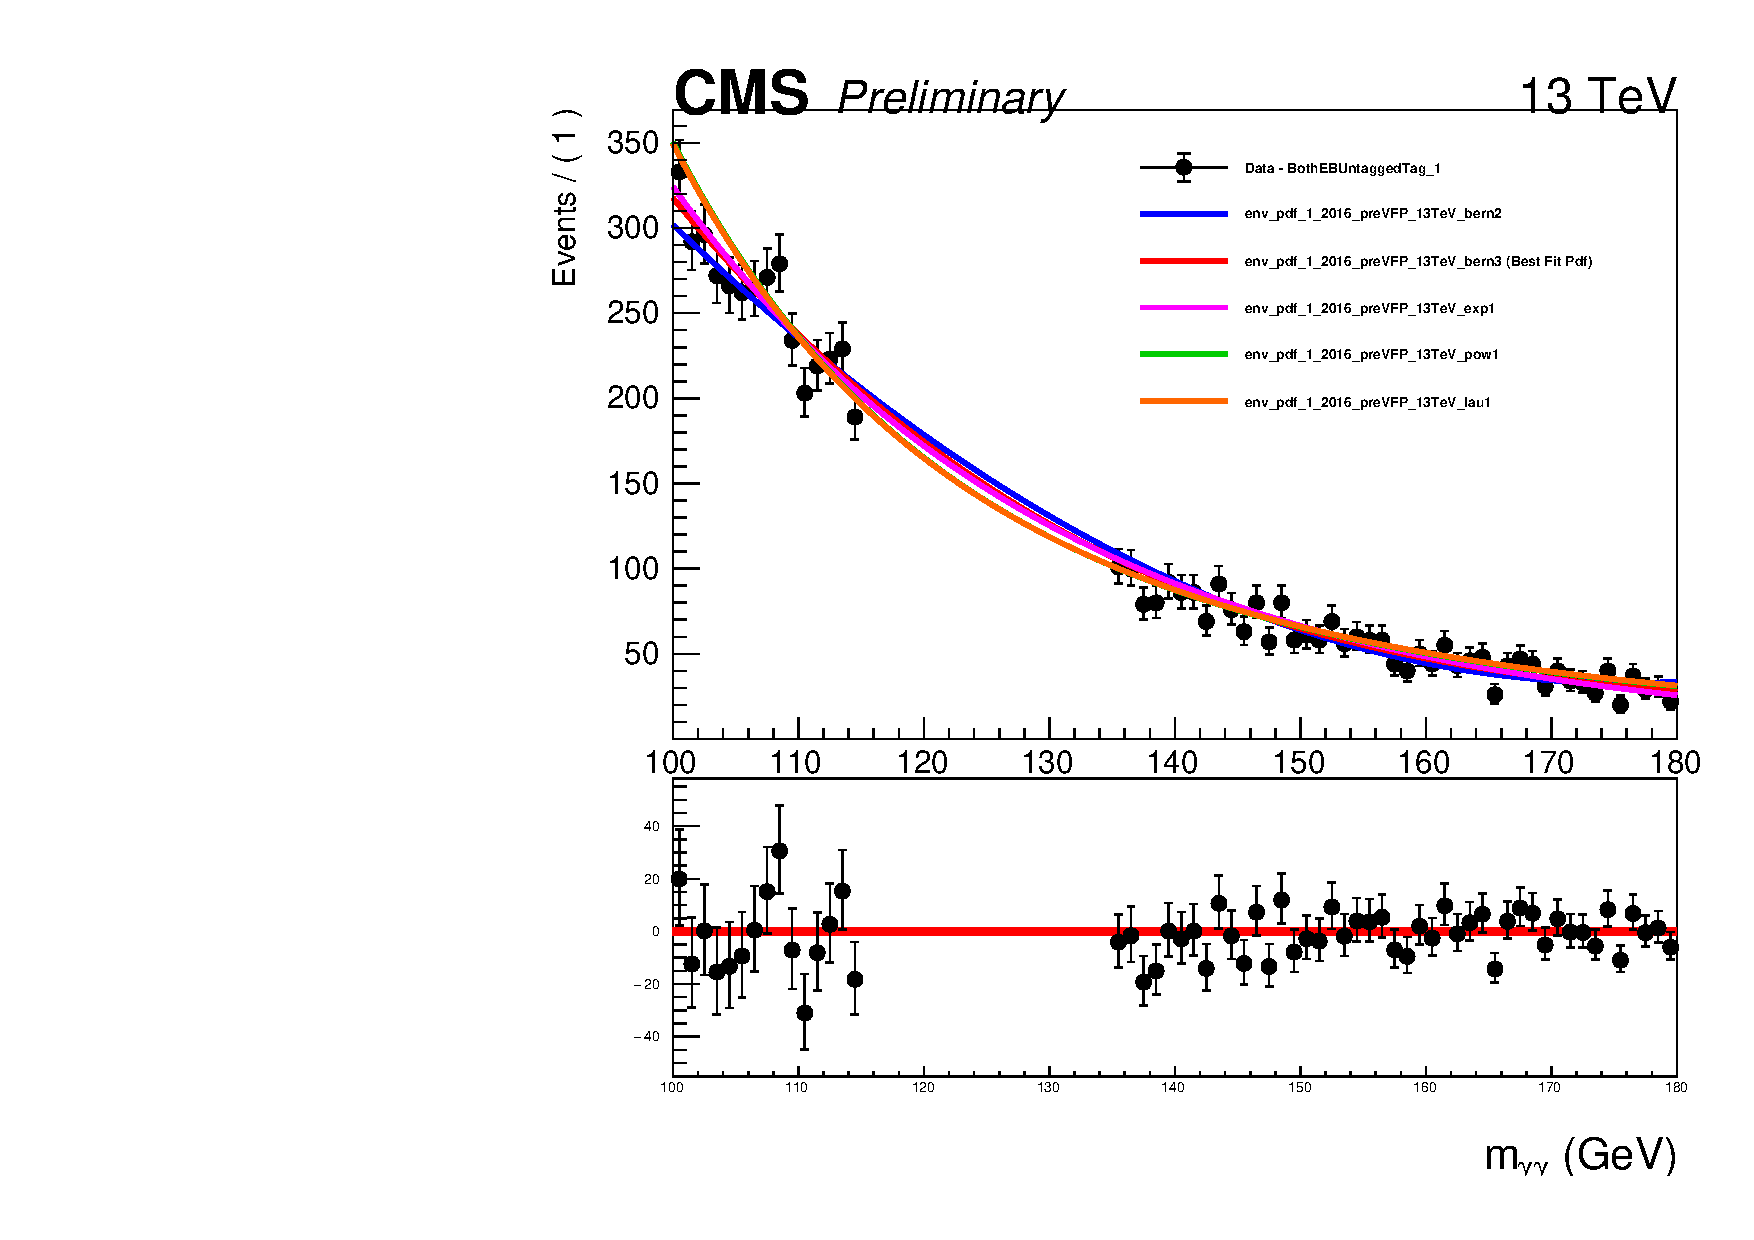
\includegraphics[width=0.925\textwidth]{07-figures/bkg_models/multipdf_BothEBUntaggedTag_1_2016preVFP.pdf}
            \end{center}
        \end{minipage}
    }~\subfloat{%
        \begin{minipage}[t]{0.5\textwidth}%
            \begin{center}
                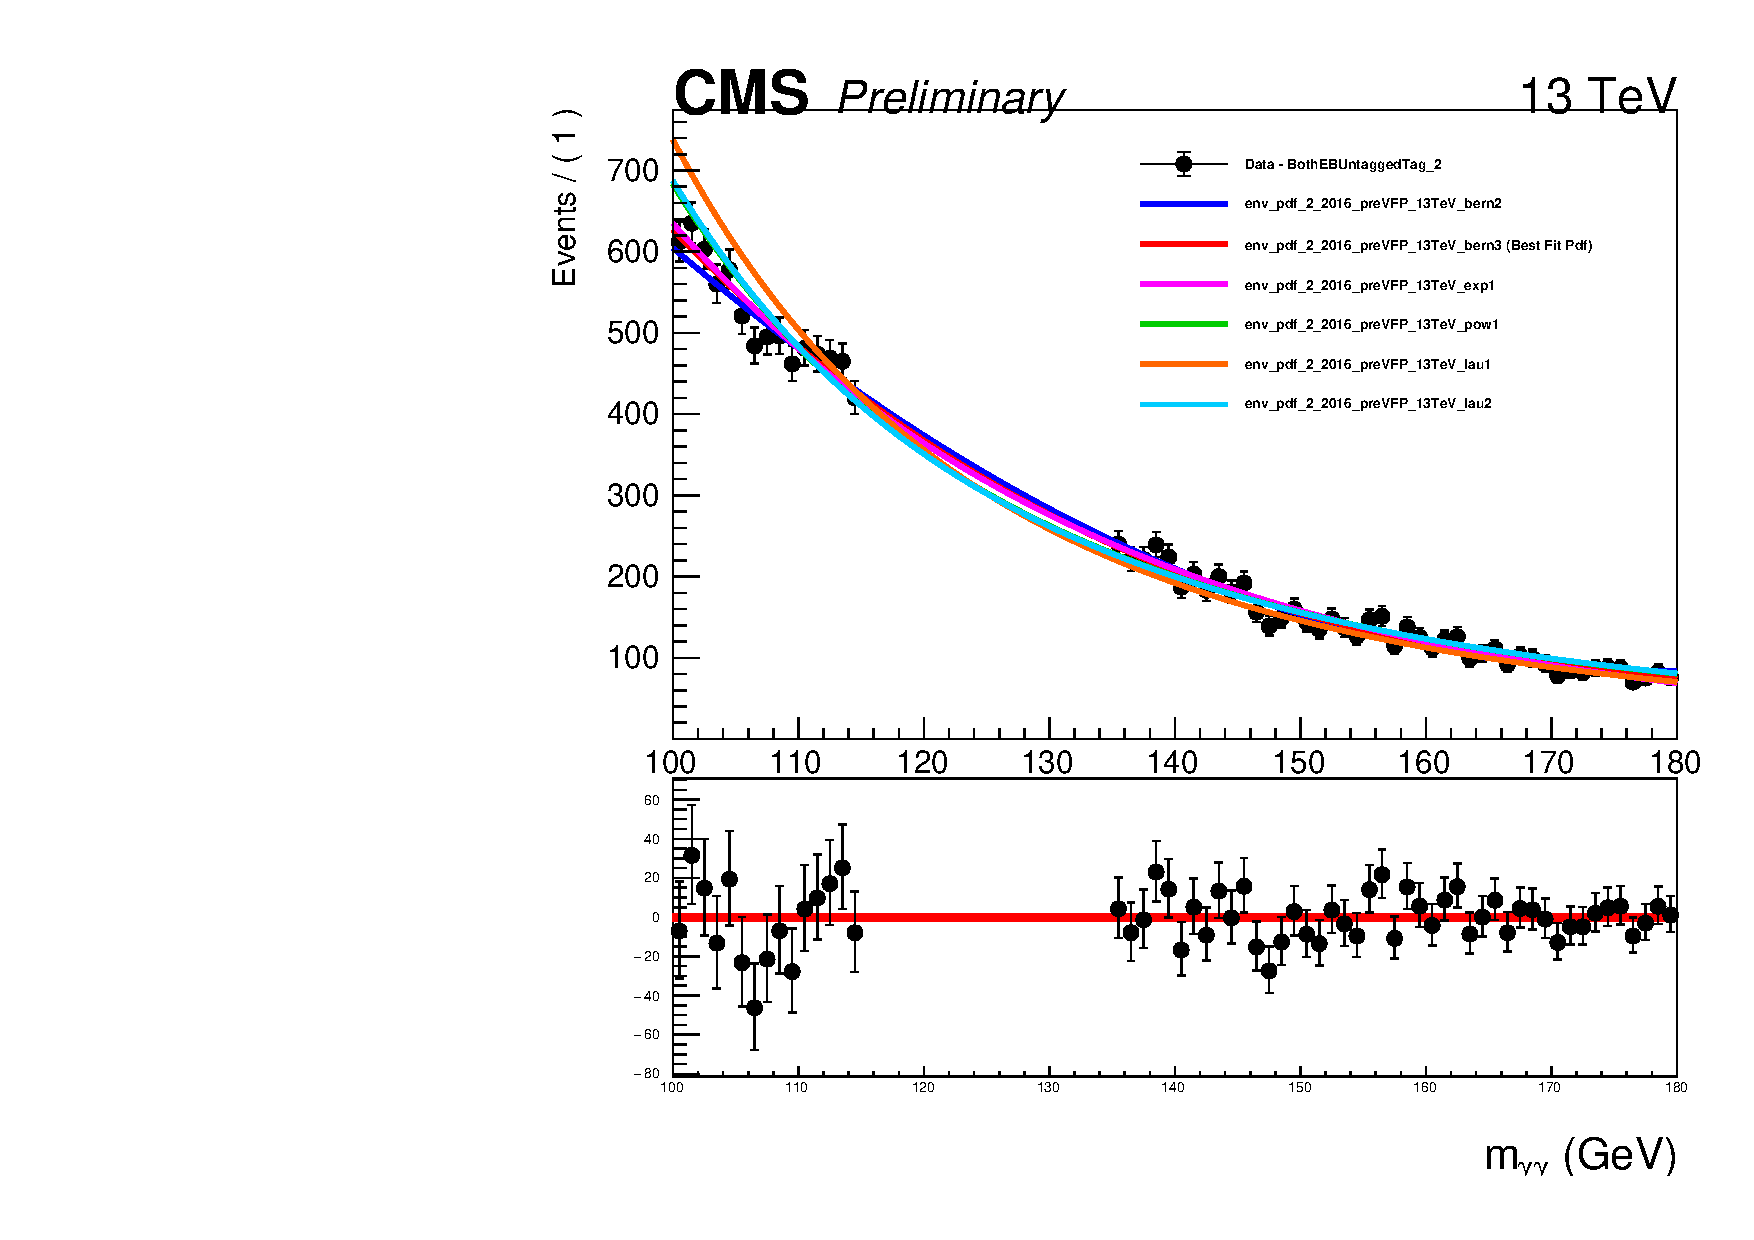
\includegraphics[width=0.925\textwidth]{07-figures/bkg_models/multipdf_BothEBUntaggedTag_2_2016preVFP.pdf}
            \end{center}
        \end{minipage}
    }~\subfloat{%
        \begin{minipage}[t]{0.5\textwidth}%
            \begin{center}
                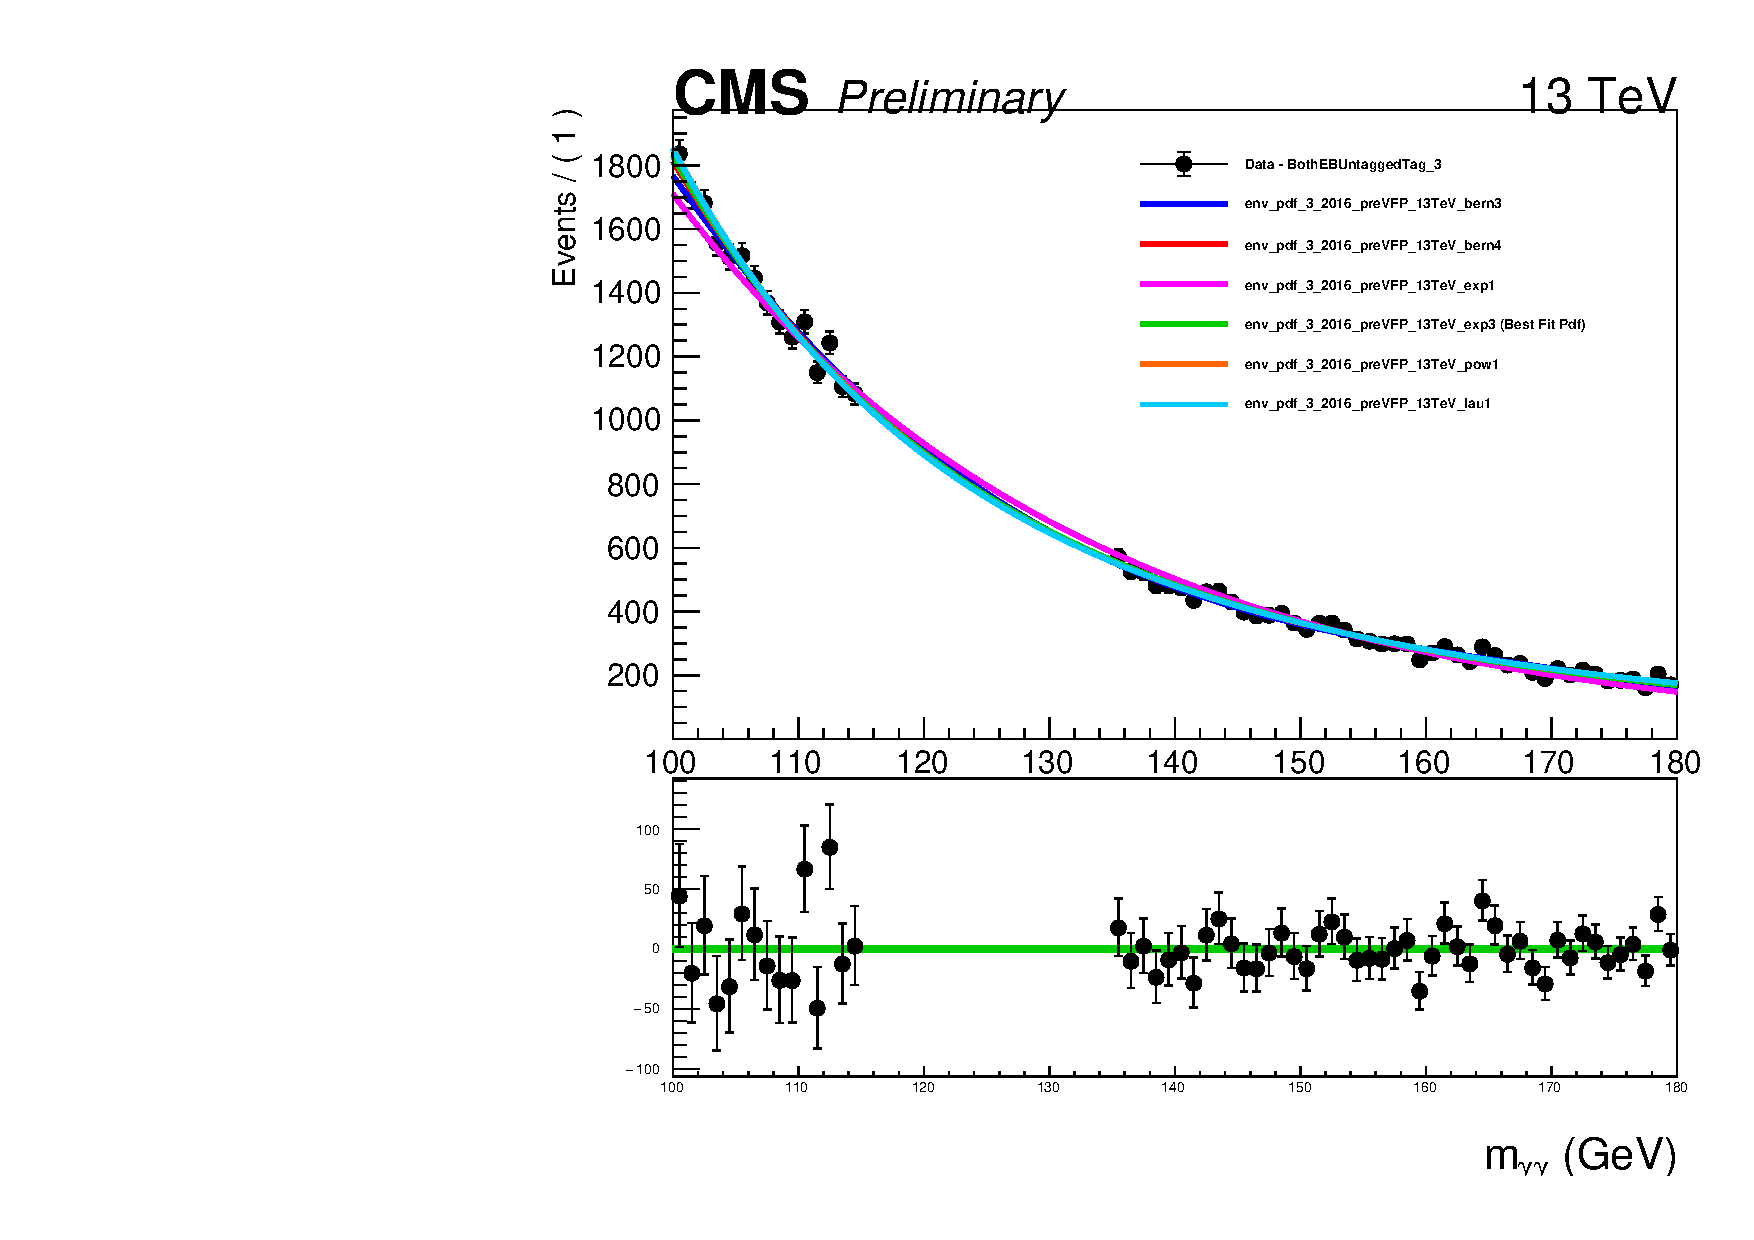
\includegraphics[width=0.925\textwidth]{07-figures/bkg_models/multipdf_BothEBUntaggedTag_3_2016preVFP.pdf}
            \end{center}
        \end{minipage}
    }
            \begin{center}
    \subfloat{%
        \begin{minipage}[t]{0.5\textwidth}%
                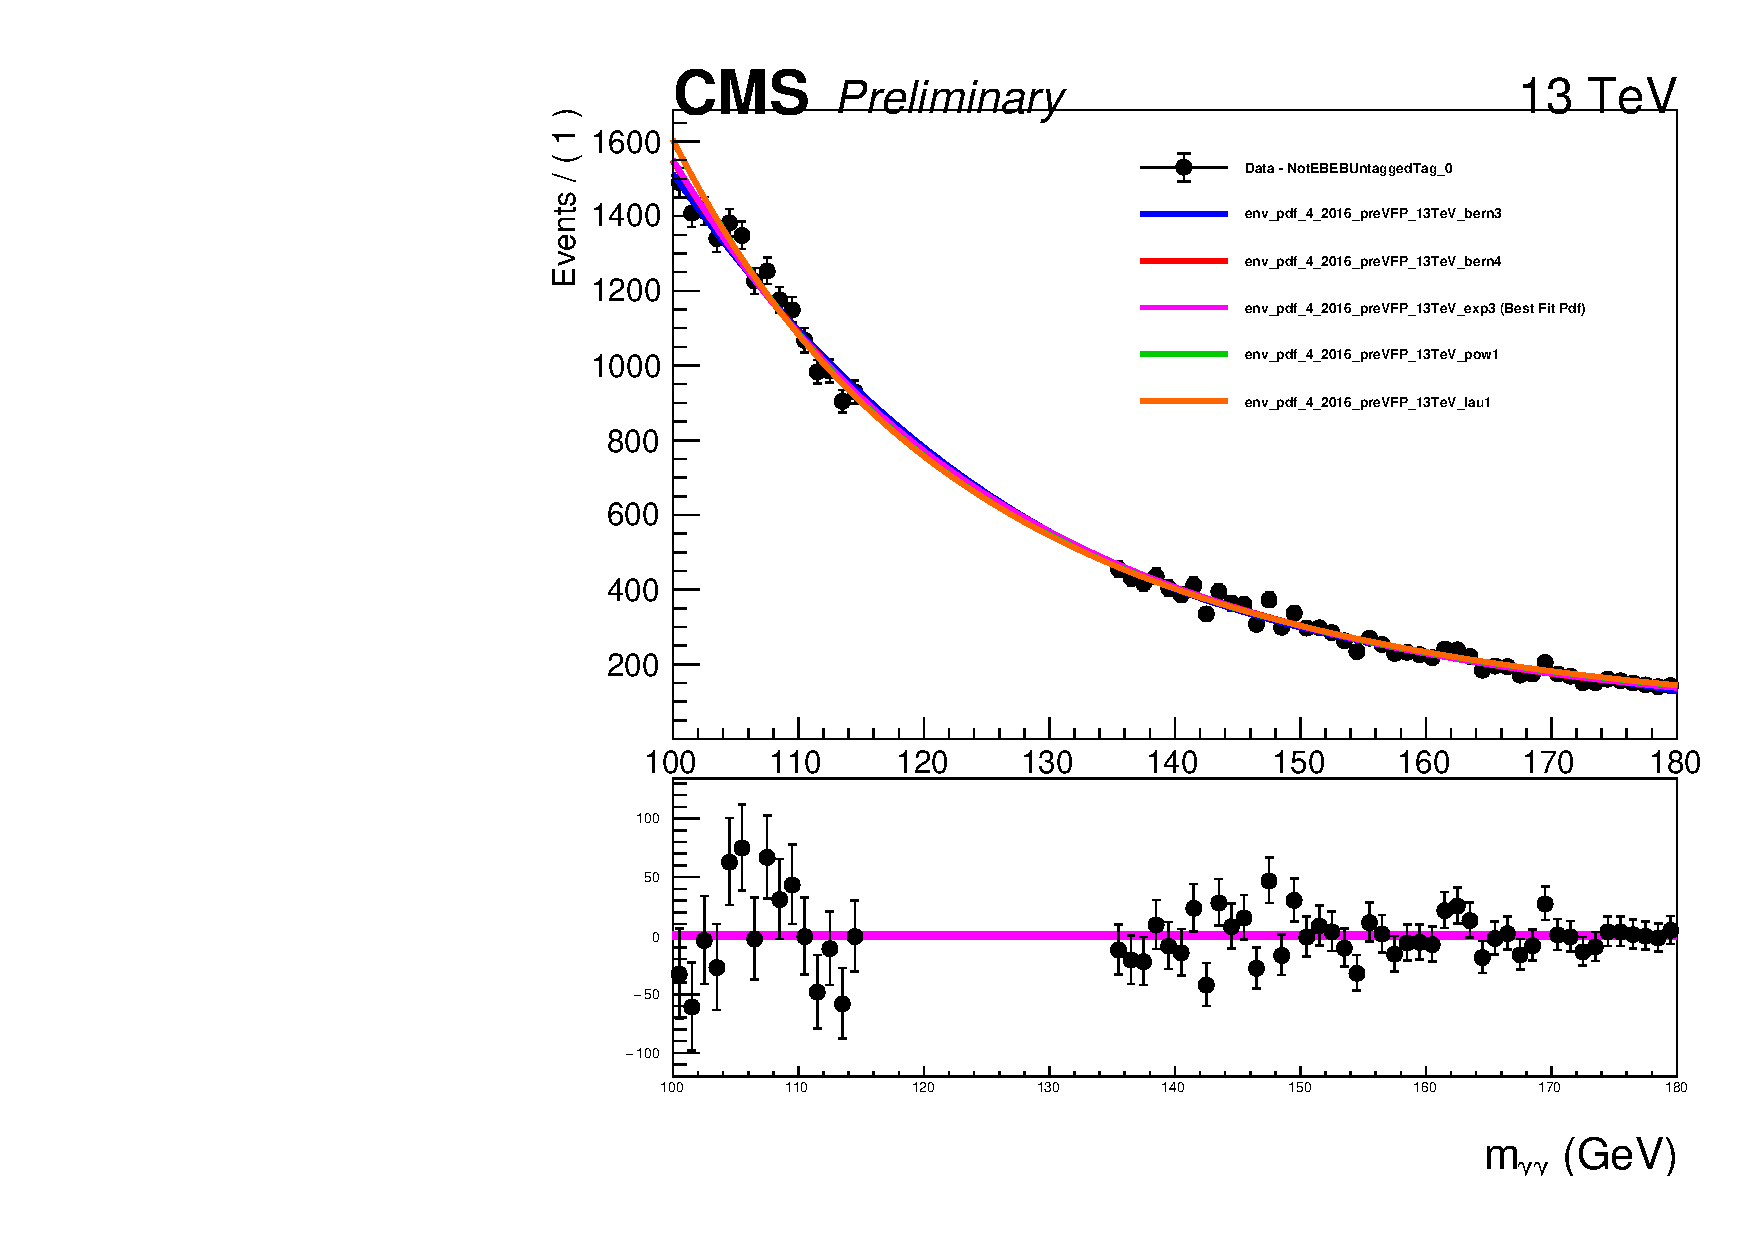
\includegraphics[width=0.925\textwidth]{07-figures/bkg_models/multipdf_NotEBEBUntaggedTag_0_2016preVFP.pdf}
        \end{minipage}
    }
            \end{center}
    \caption[Background models: 2016 preVFP]{Background models for 2016 preVFP in each category.}
    \label{fig:bkg_model_2016_preVFP}
\end{figure}

\begin{figure}[htbp!]
    \subfloat{%
        \begin{minipage}[t]{0.5\textwidth}%
            \begin{center}
                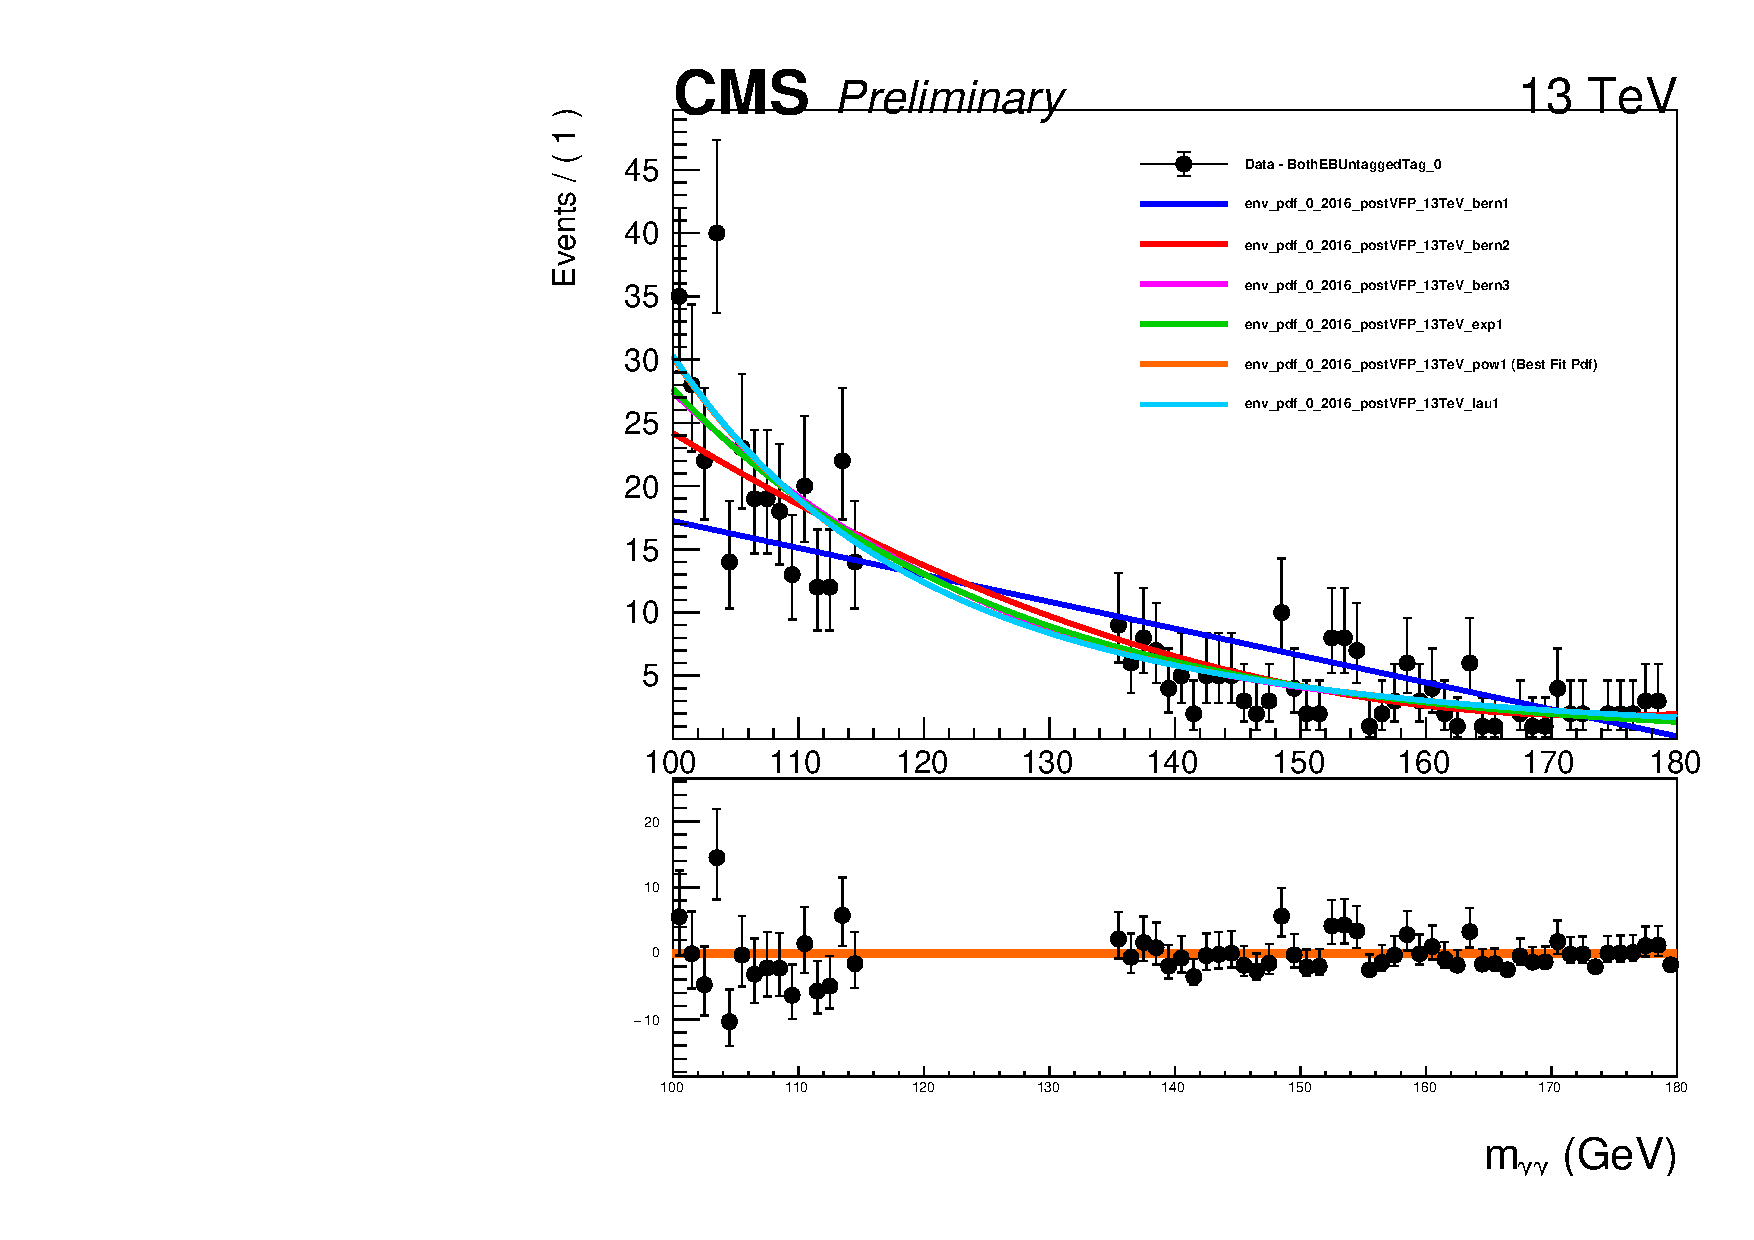
\includegraphics[width=0.925\textwidth]{07-figures/bkg_models/multipdf_BothEBUntaggedTag_0_2016postVFP.pdf}
            \end{center}
        \end{minipage}
    }~\subfloat{%
        \begin{minipage}[t]{0.5\textwidth}%
            \begin{center}
                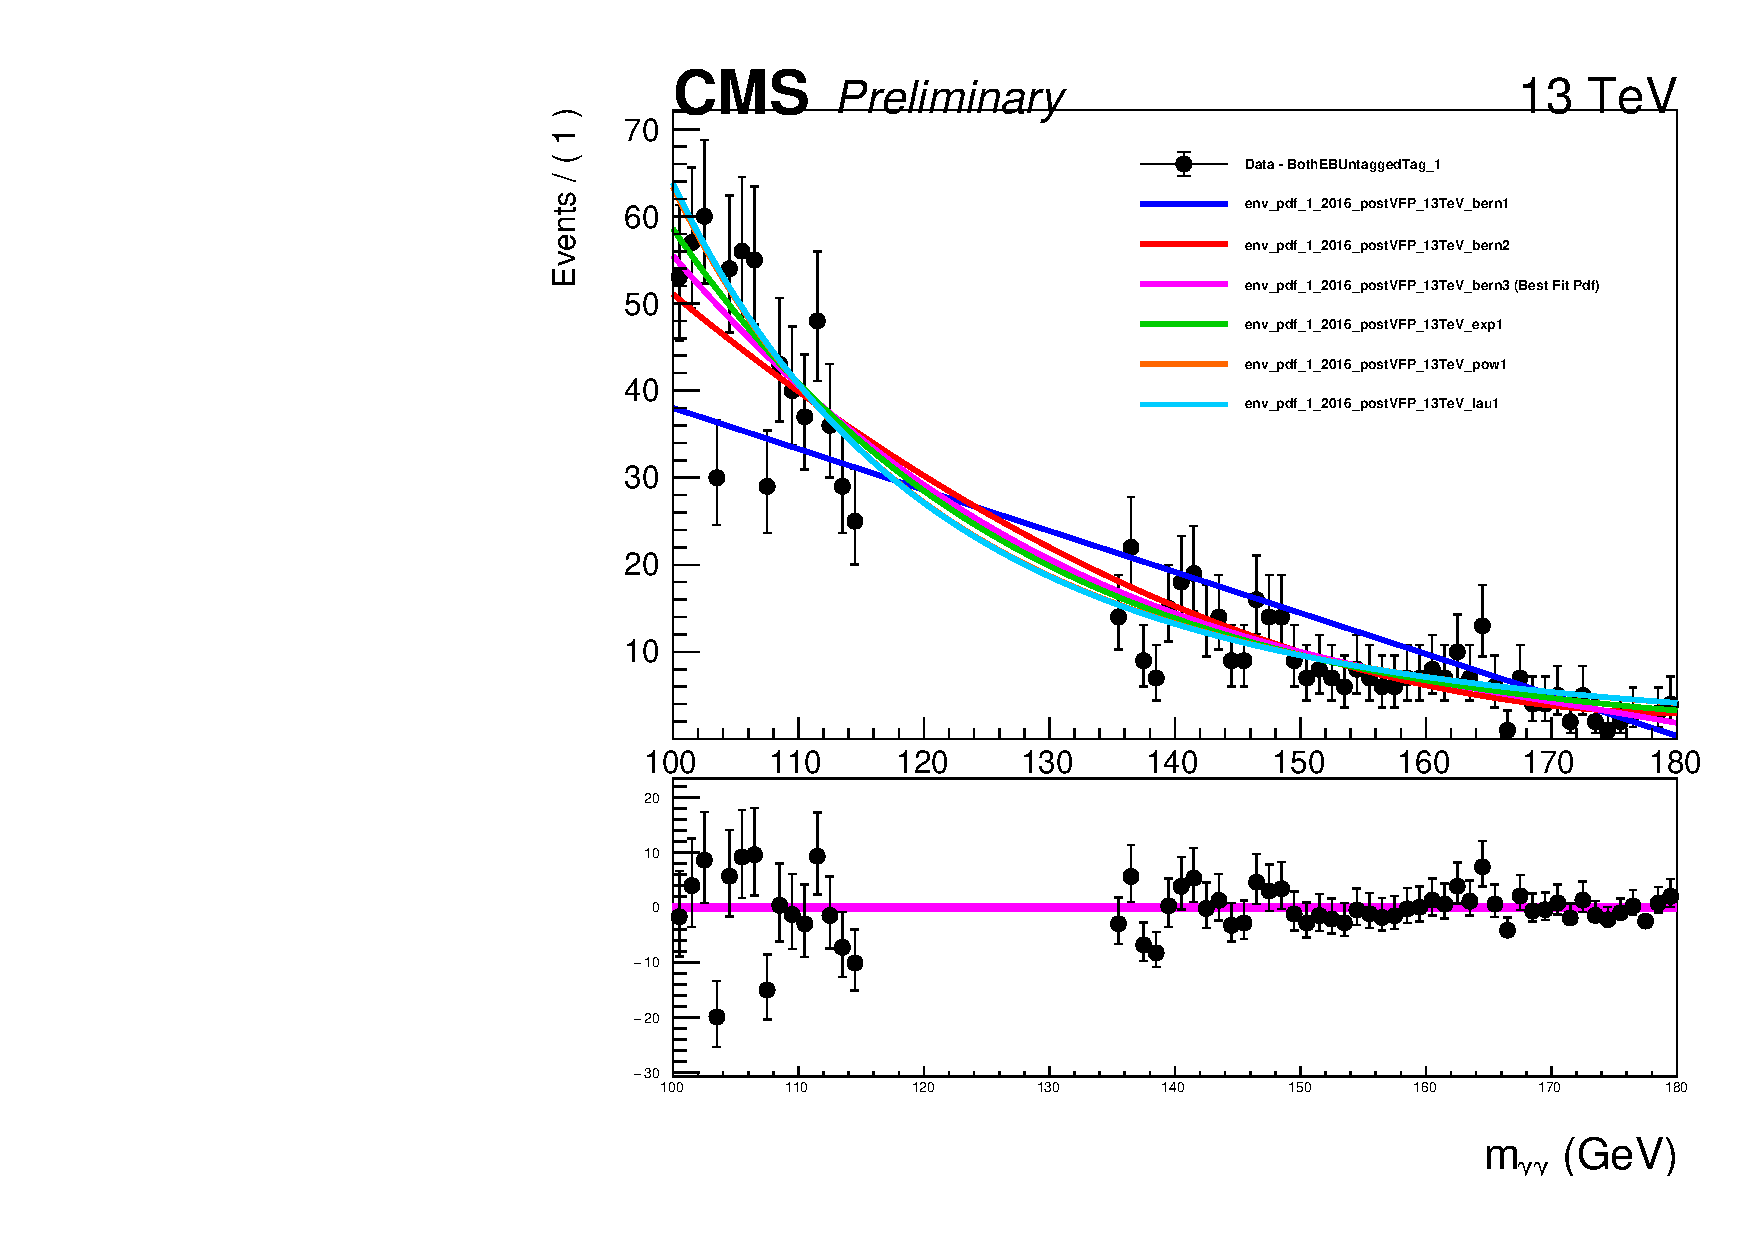
\includegraphics[width=0.925\textwidth]{07-figures/bkg_models/multipdf_BothEBUntaggedTag_1_2016postVFP.pdf}
            \end{center}
        \end{minipage}
    }~\subfloat{%
        \begin{minipage}[t]{0.5\textwidth}%
            \begin{center}
                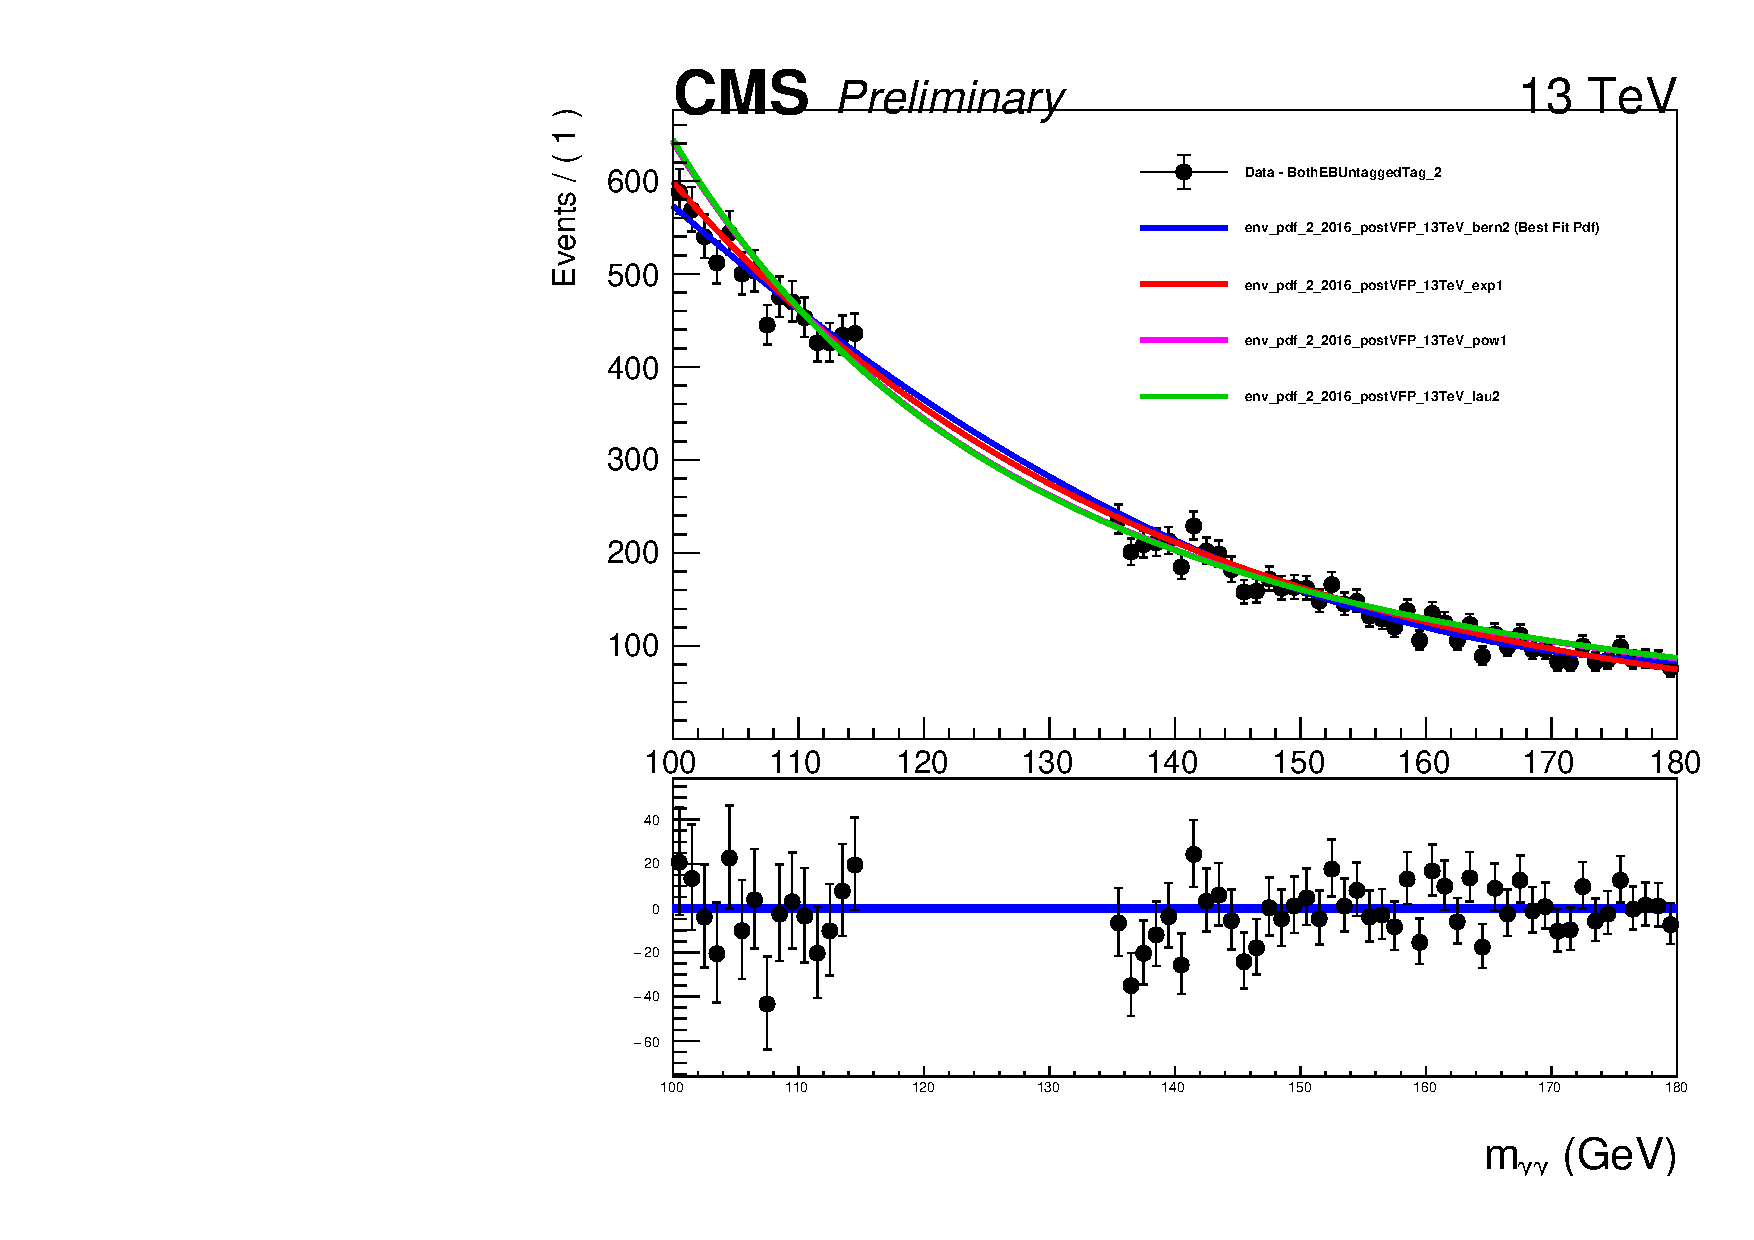
\includegraphics[width=0.925\textwidth]{07-figures/bkg_models/multipdf_BothEBUntaggedTag_2_2016postVFP.pdf}
            \end{center}
        \end{minipage}
    }~\subfloat{%
        \begin{minipage}[t]{0.5\textwidth}%
            \begin{center}
                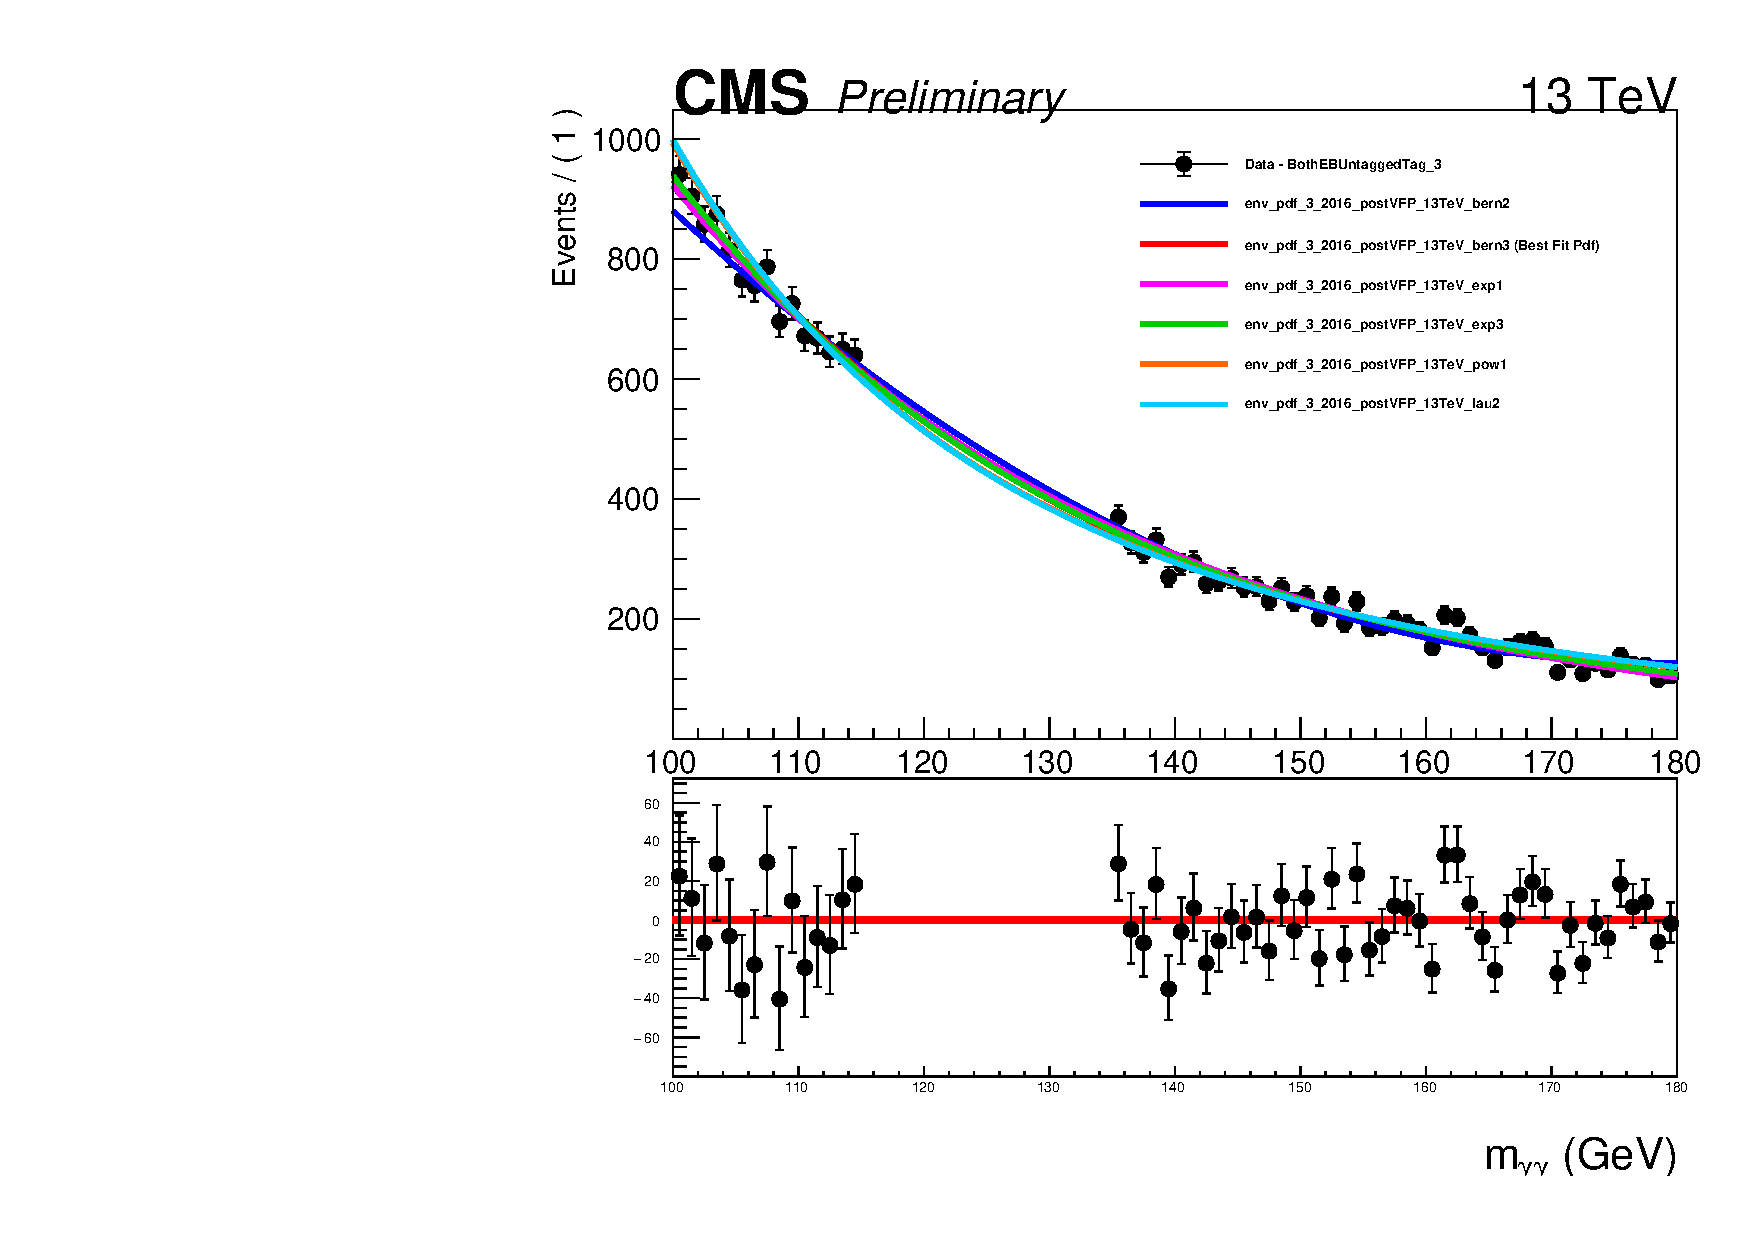
\includegraphics[width=0.952\textwidth]{07-figures/bkg_models/multipdf_BothEBUntaggedTag_3_2016postVFP.pdf}
            \end{center}
        \end{minipage}
    }
            \begin{center}
    \subfloat{%
        \begin{minipage}[t]{0.5\textwidth}%
                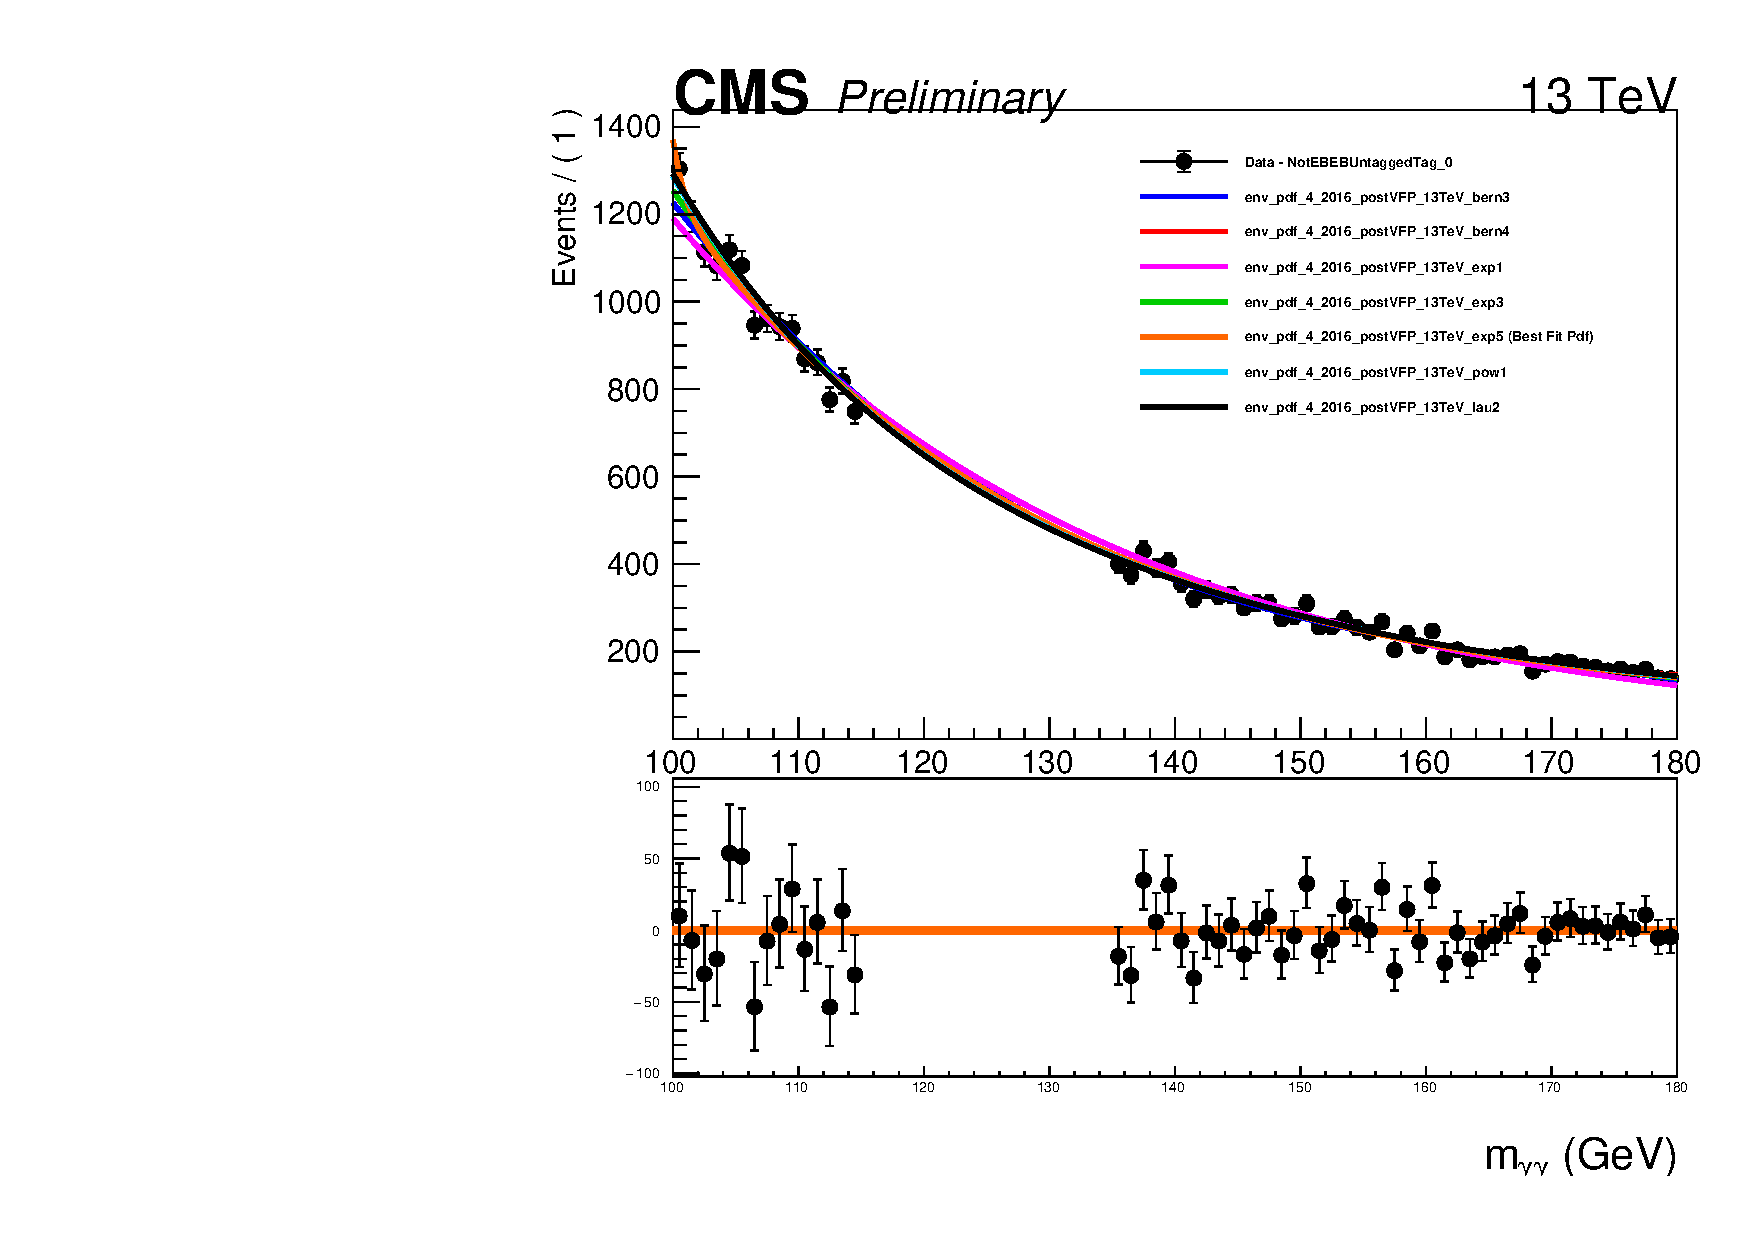
\includegraphics[width=0.925\textwidth]{07-figures/bkg_models/multipdf_NotEBEBUntaggedTag_0_2016postVFP.pdf}
        \end{minipage}
    }
            \end{center}
    \caption[Background models: 2016 postVFP]{Background models for 2016 postVFP in each category.}
    \label{fig:bkg_model_2016_postVFP}
\end{figure}

\begin{figure}[htbp!]
    \subfloat{%
        \begin{minipage}[t]{0.5\textwidth}%
            \begin{center}
                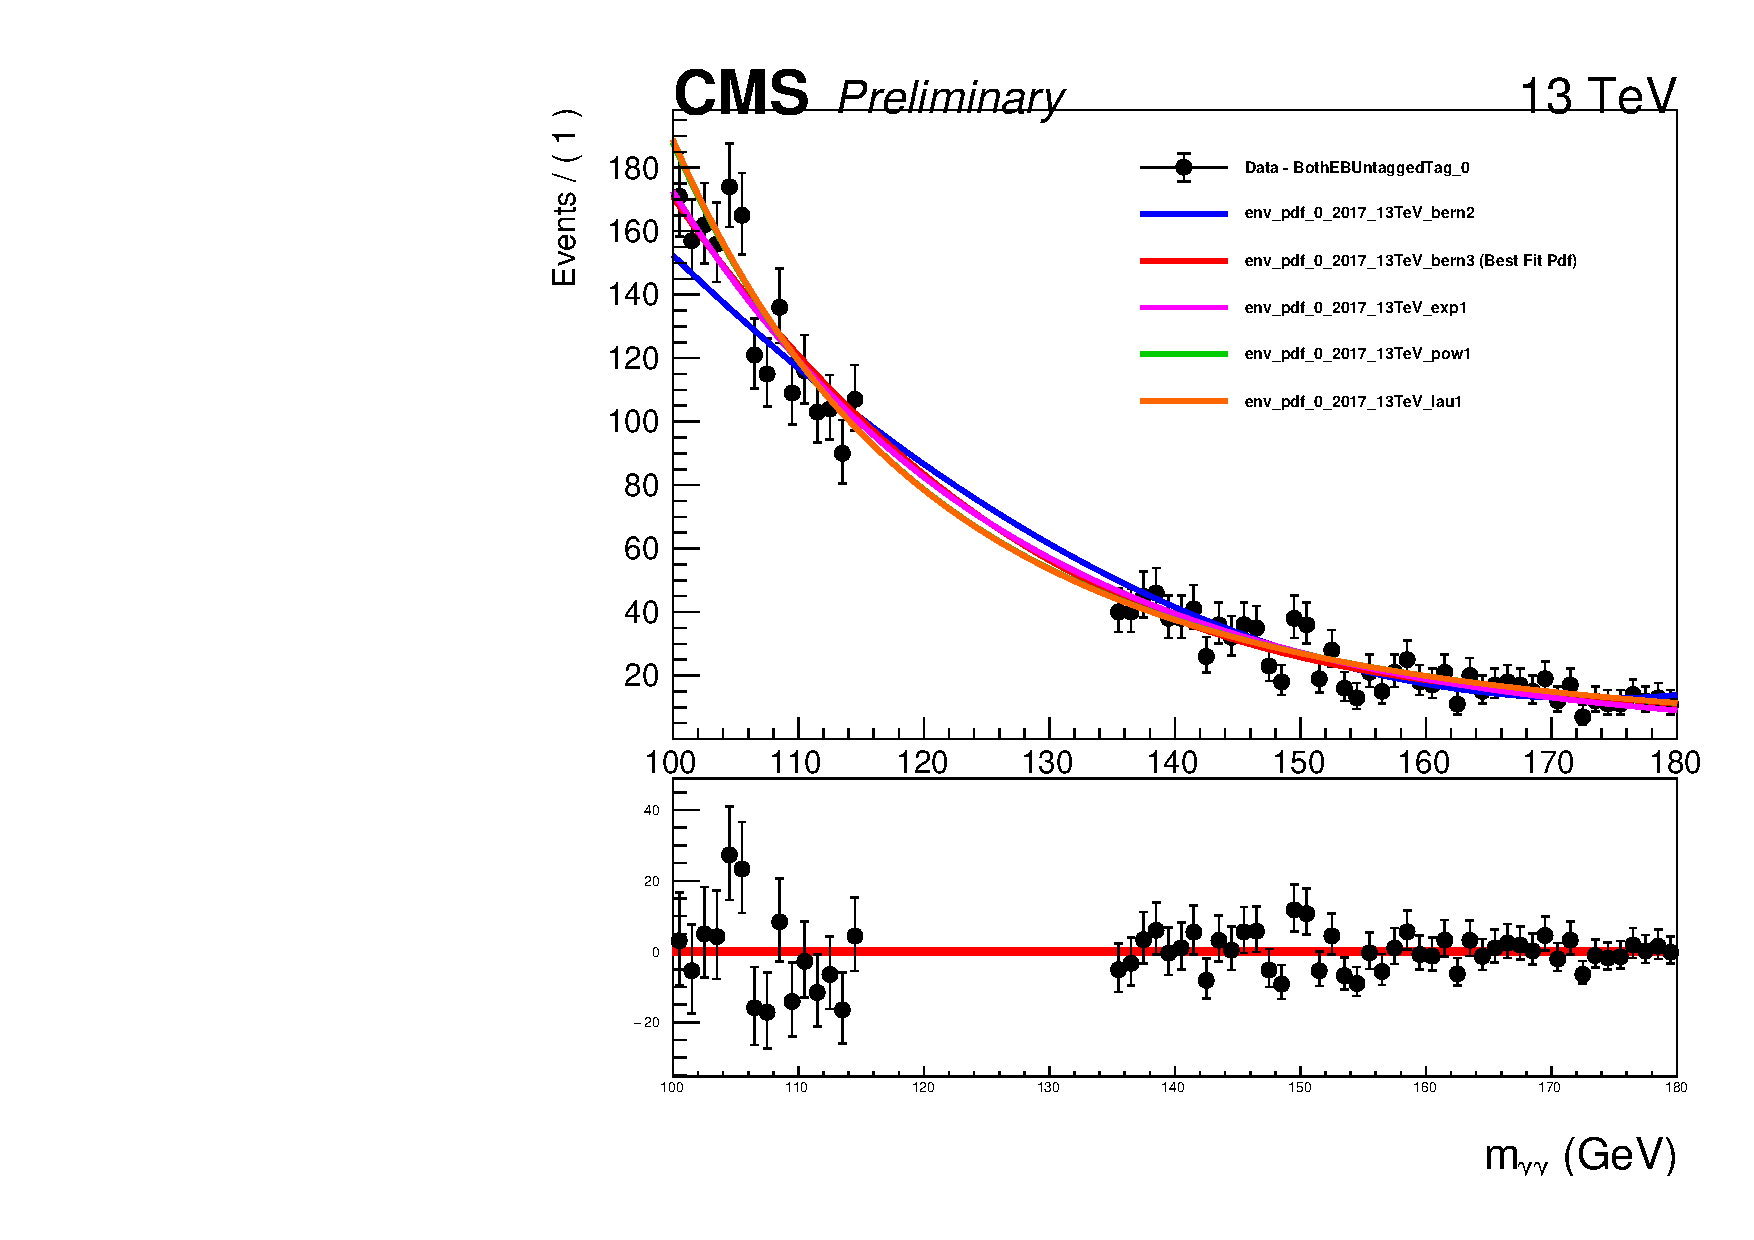
\includegraphics[width=0.925\textwidth]{07-figures/bkg_models/multipdf_BothEBUntaggedTag_0_2017.pdf}
            \end{center}
        \end{minipage}
    }~\subfloat{%
        \begin{minipage}[t]{0.5\textwidth}%
            \begin{center}
                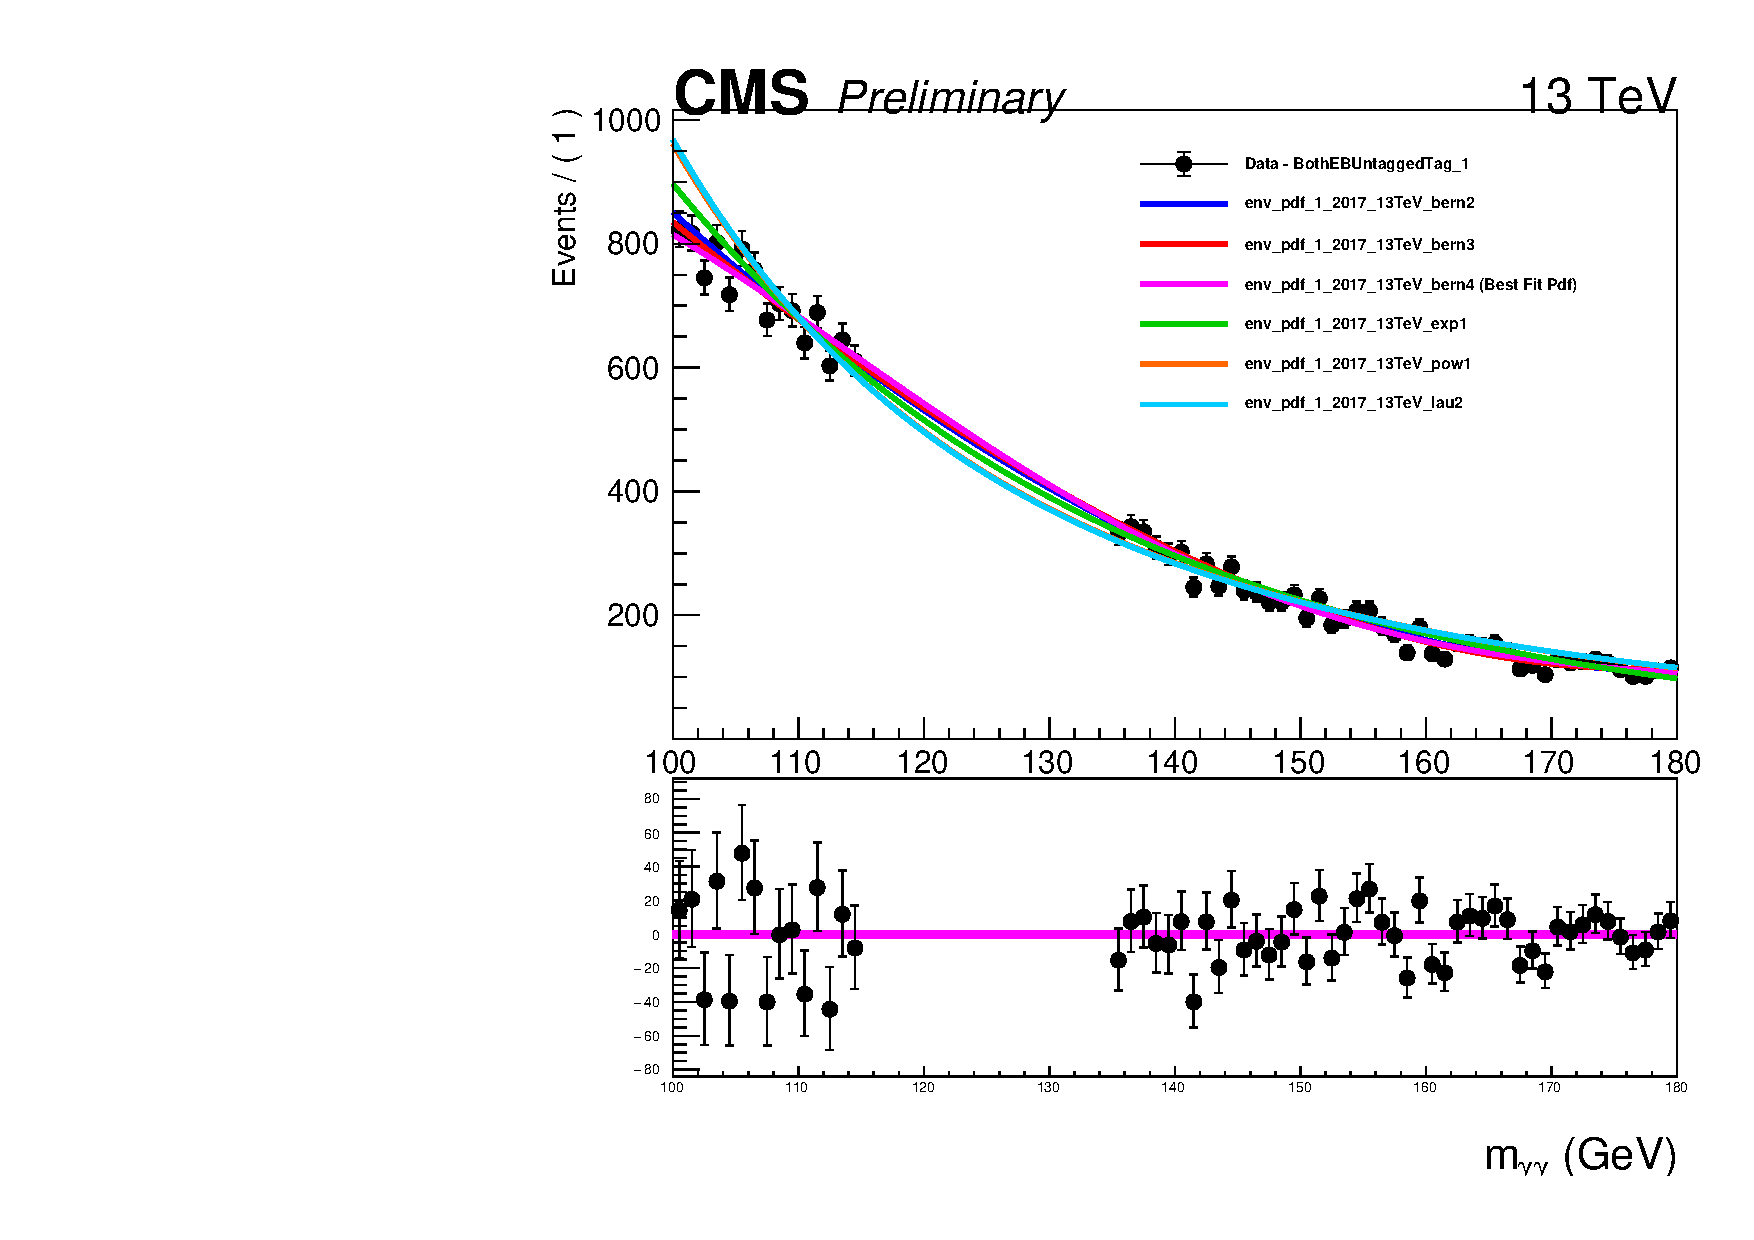
\includegraphics[width=0.925\textwidth]{07-figures/bkg_models/multipdf_BothEBUntaggedTag_1_2017.pdf}
            \end{center}
        \end{minipage}
    }~\subfloat{%
        \begin{minipage}[t]{0.5\textwidth}%
            \begin{center}
                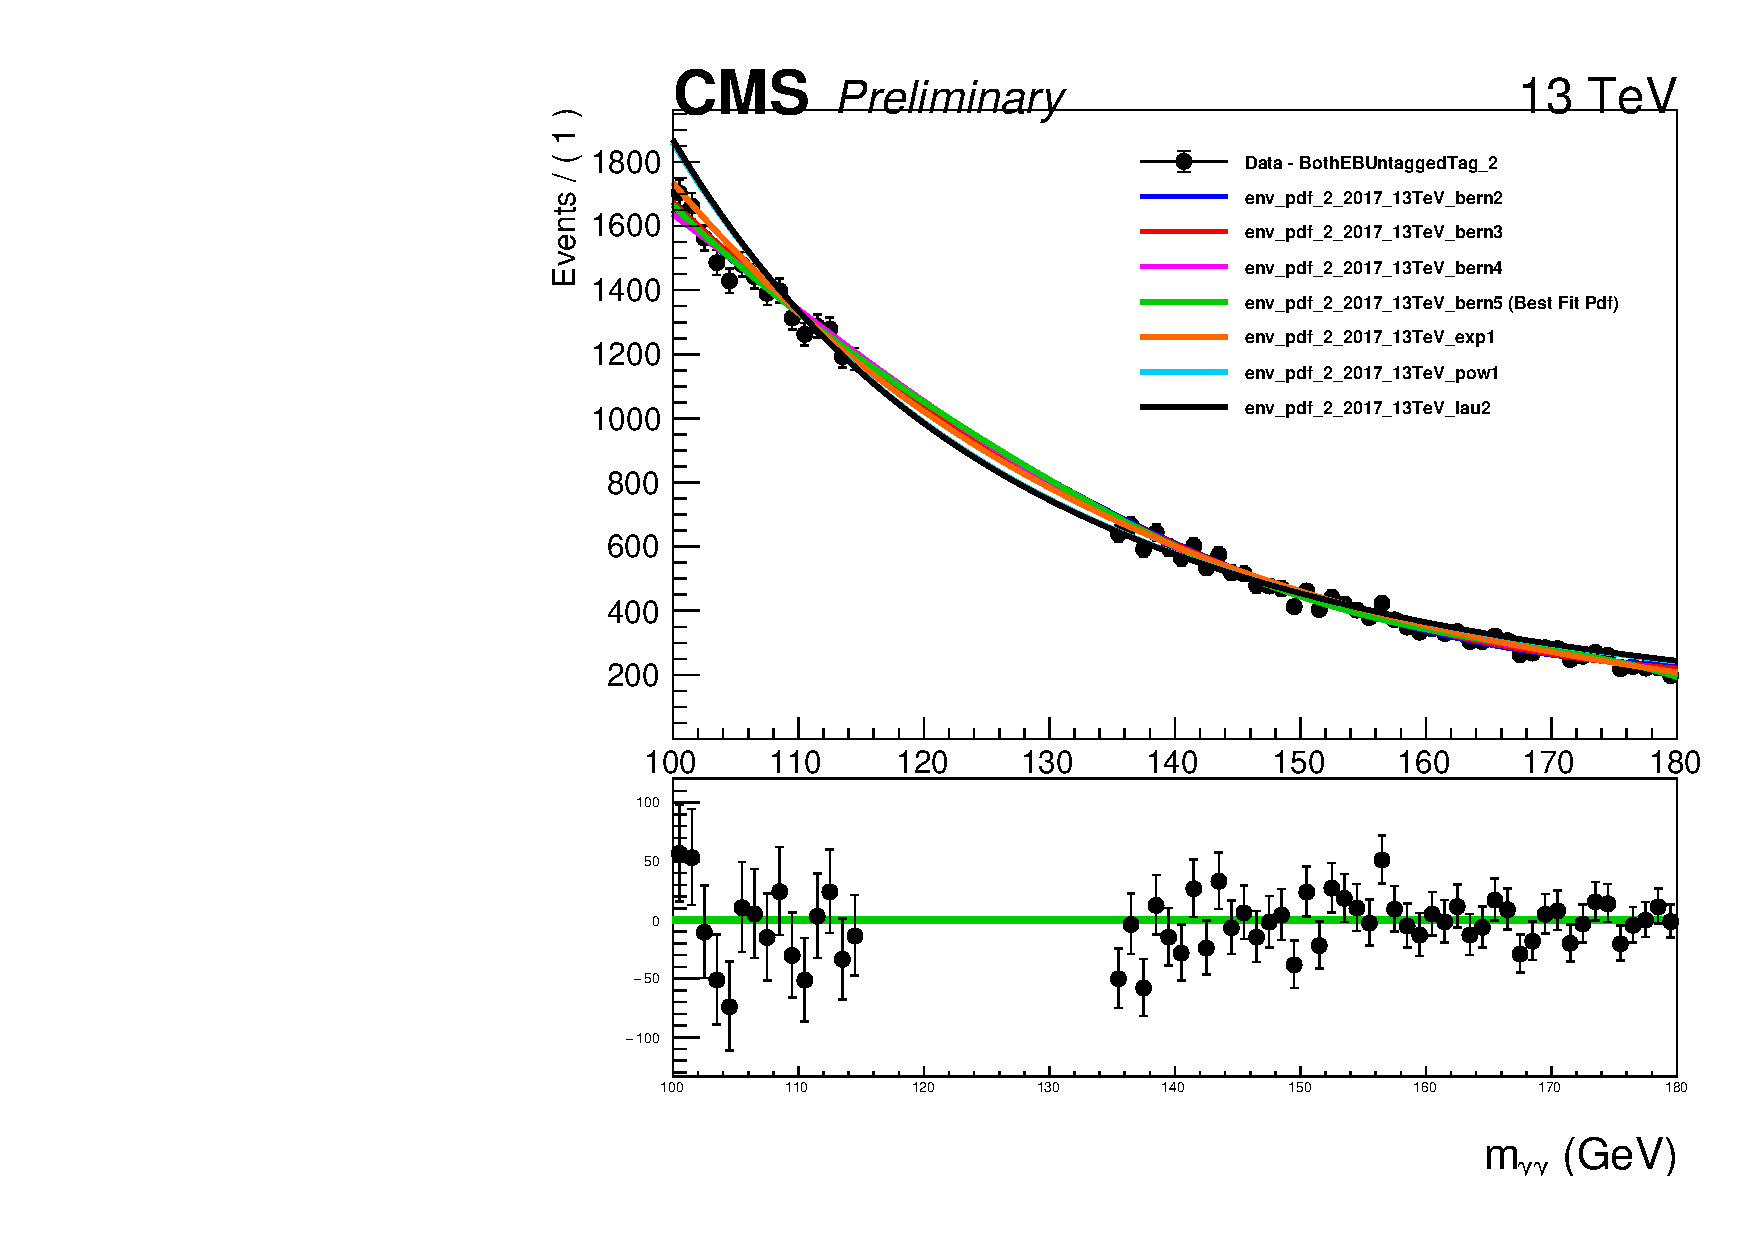
\includegraphics[width=0.925\textwidth]{07-figures/bkg_models/multipdf_BothEBUntaggedTag_2_2017.pdf}
            \end{center}
        \end{minipage}
    }~\subfloat{%
        \begin{minipage}[t]{0.5\textwidth}%
            \begin{center}
                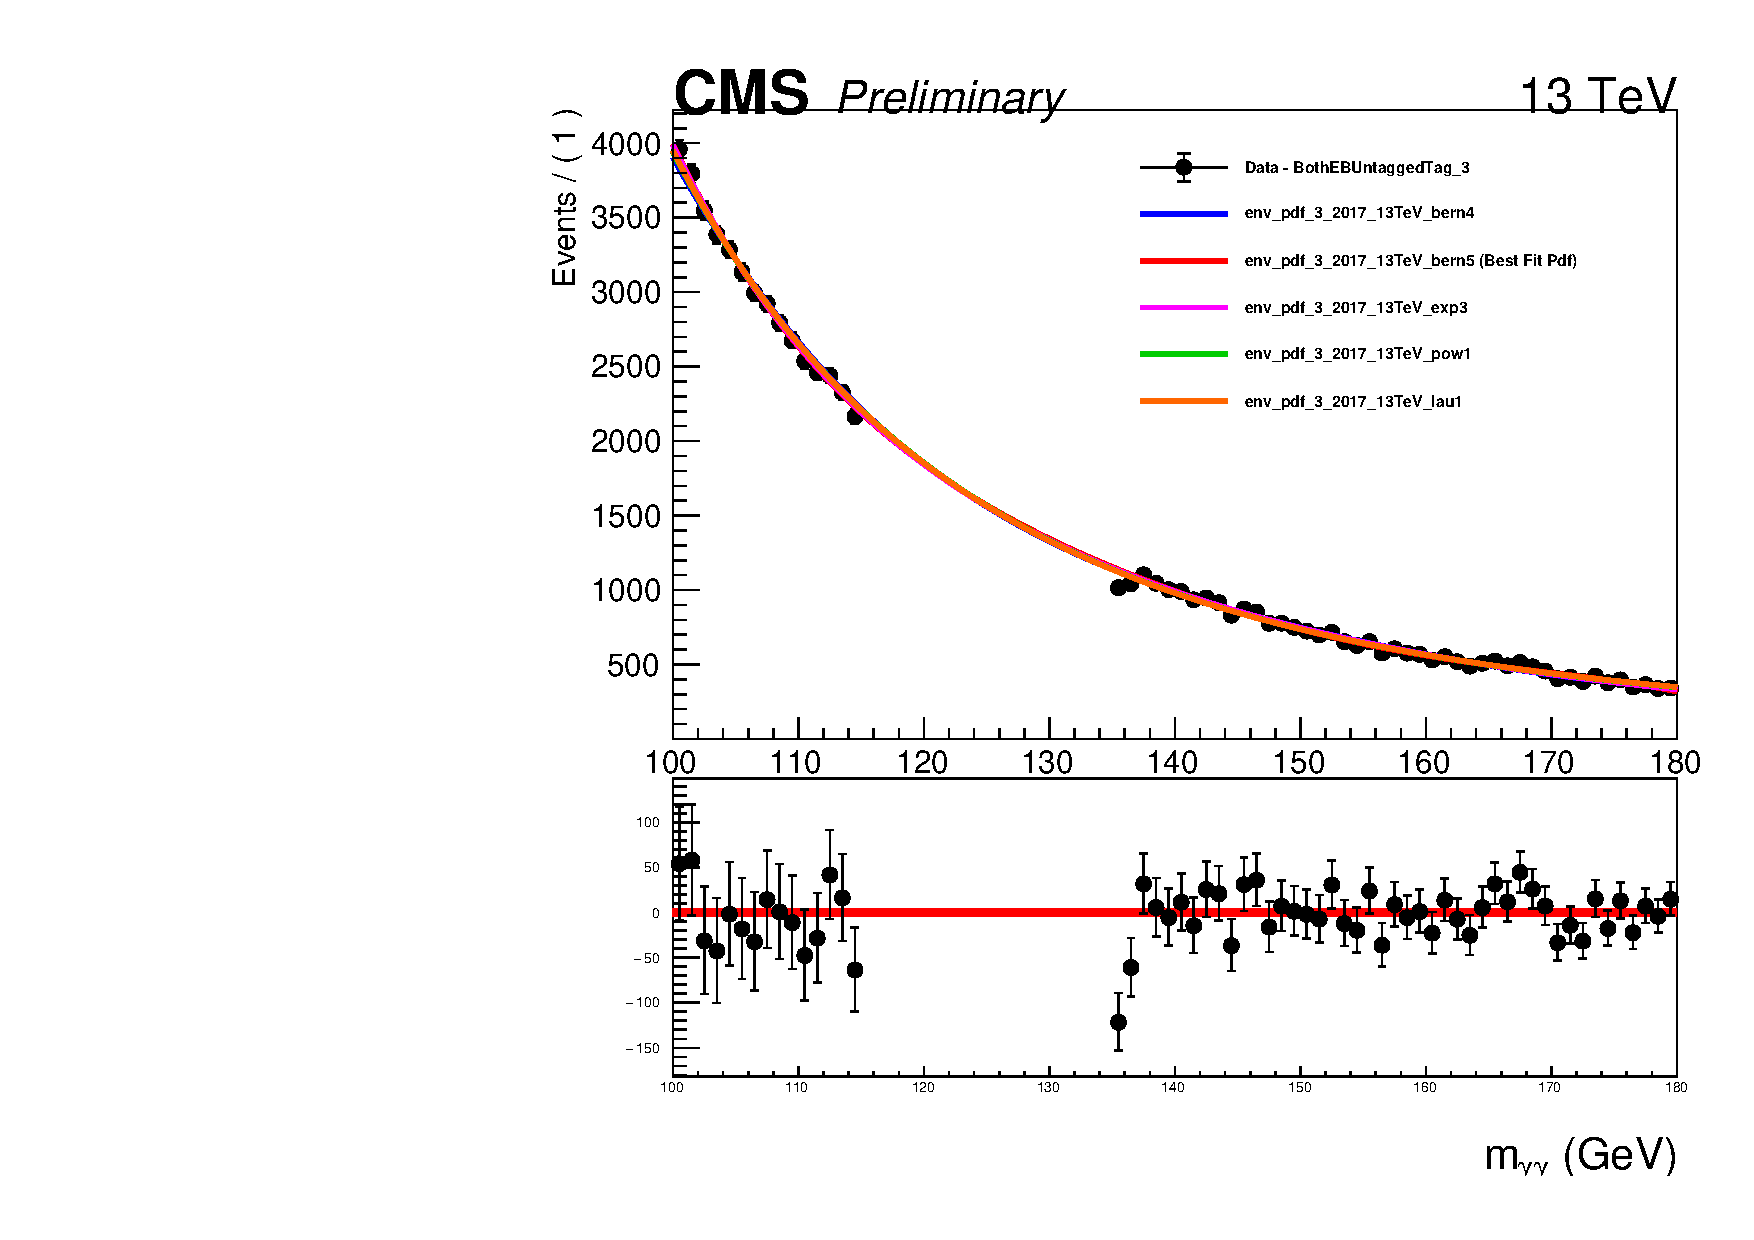
\includegraphics[width=0.925\textwidth]{07-figures/bkg_models/multipdf_BothEBUntaggedTag_3_2017.pdf}
            \end{center}
        \end{minipage}
    }
            \begin{center}
    \subfloat{%
        \begin{minipage}[t]{0.5\textwidth}%
                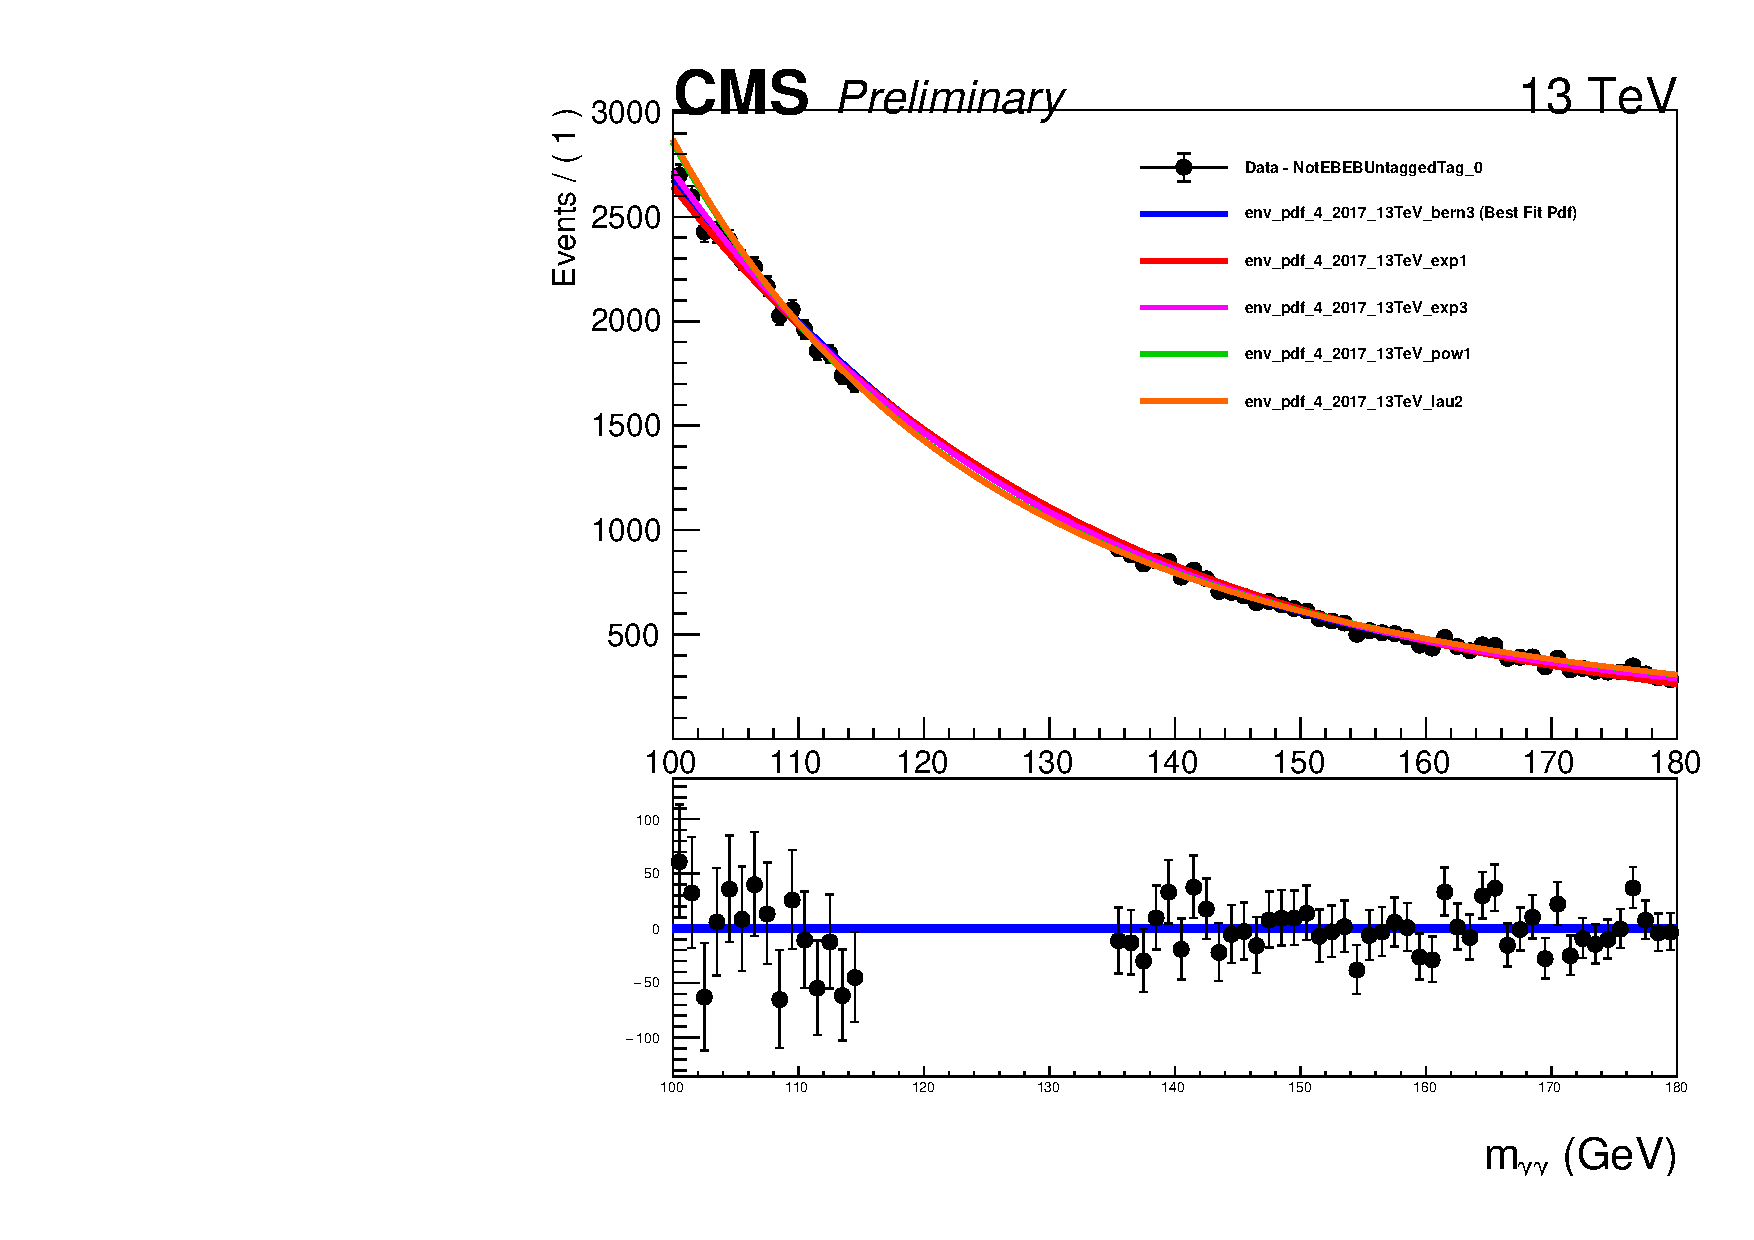
\includegraphics[width=0.925\textwidth]{07-figures/bkg_models/multipdf_NotEBEBUntaggedTag_0_2017.pdf}
        \end{minipage}
    }
            \end{center}
    \caption[Background models: 2017]{Background models for 2017 in each category.}
    \label{fig:bkg_model_2017}
\end{figure}

\begin{figure}[htbp!]
    \subfloat{%
        \begin{minipage}[t]{0.5\textwidth}%
            \begin{center}
                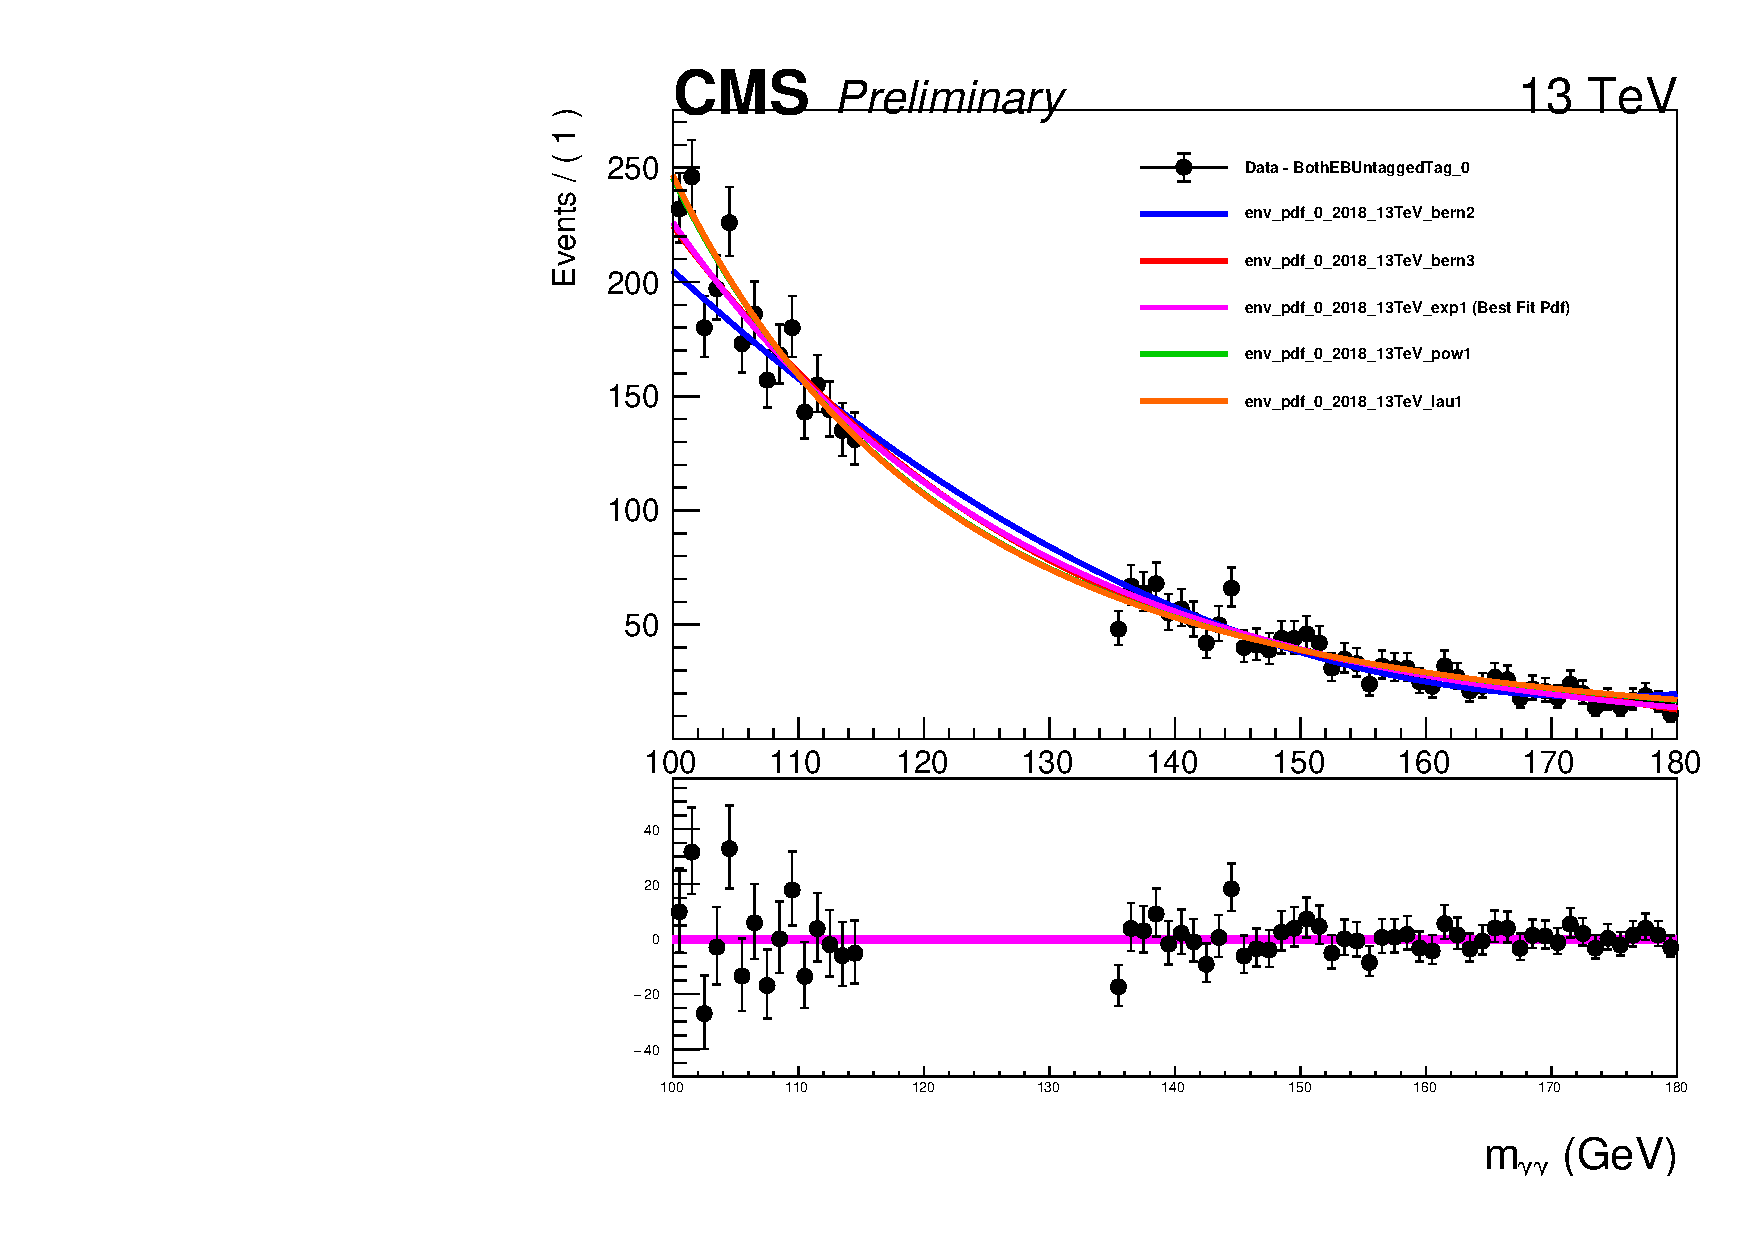
\includegraphics[width=0.925\textwidth]{07-figures/bkg_models/multipdf_BothEBUntaggedTag_0_2018.pdf}
            \end{center}
        \end{minipage}
    }~\subfloat{%
        \begin{minipage}[t]{0.5\textwidth}%
            \begin{center}
                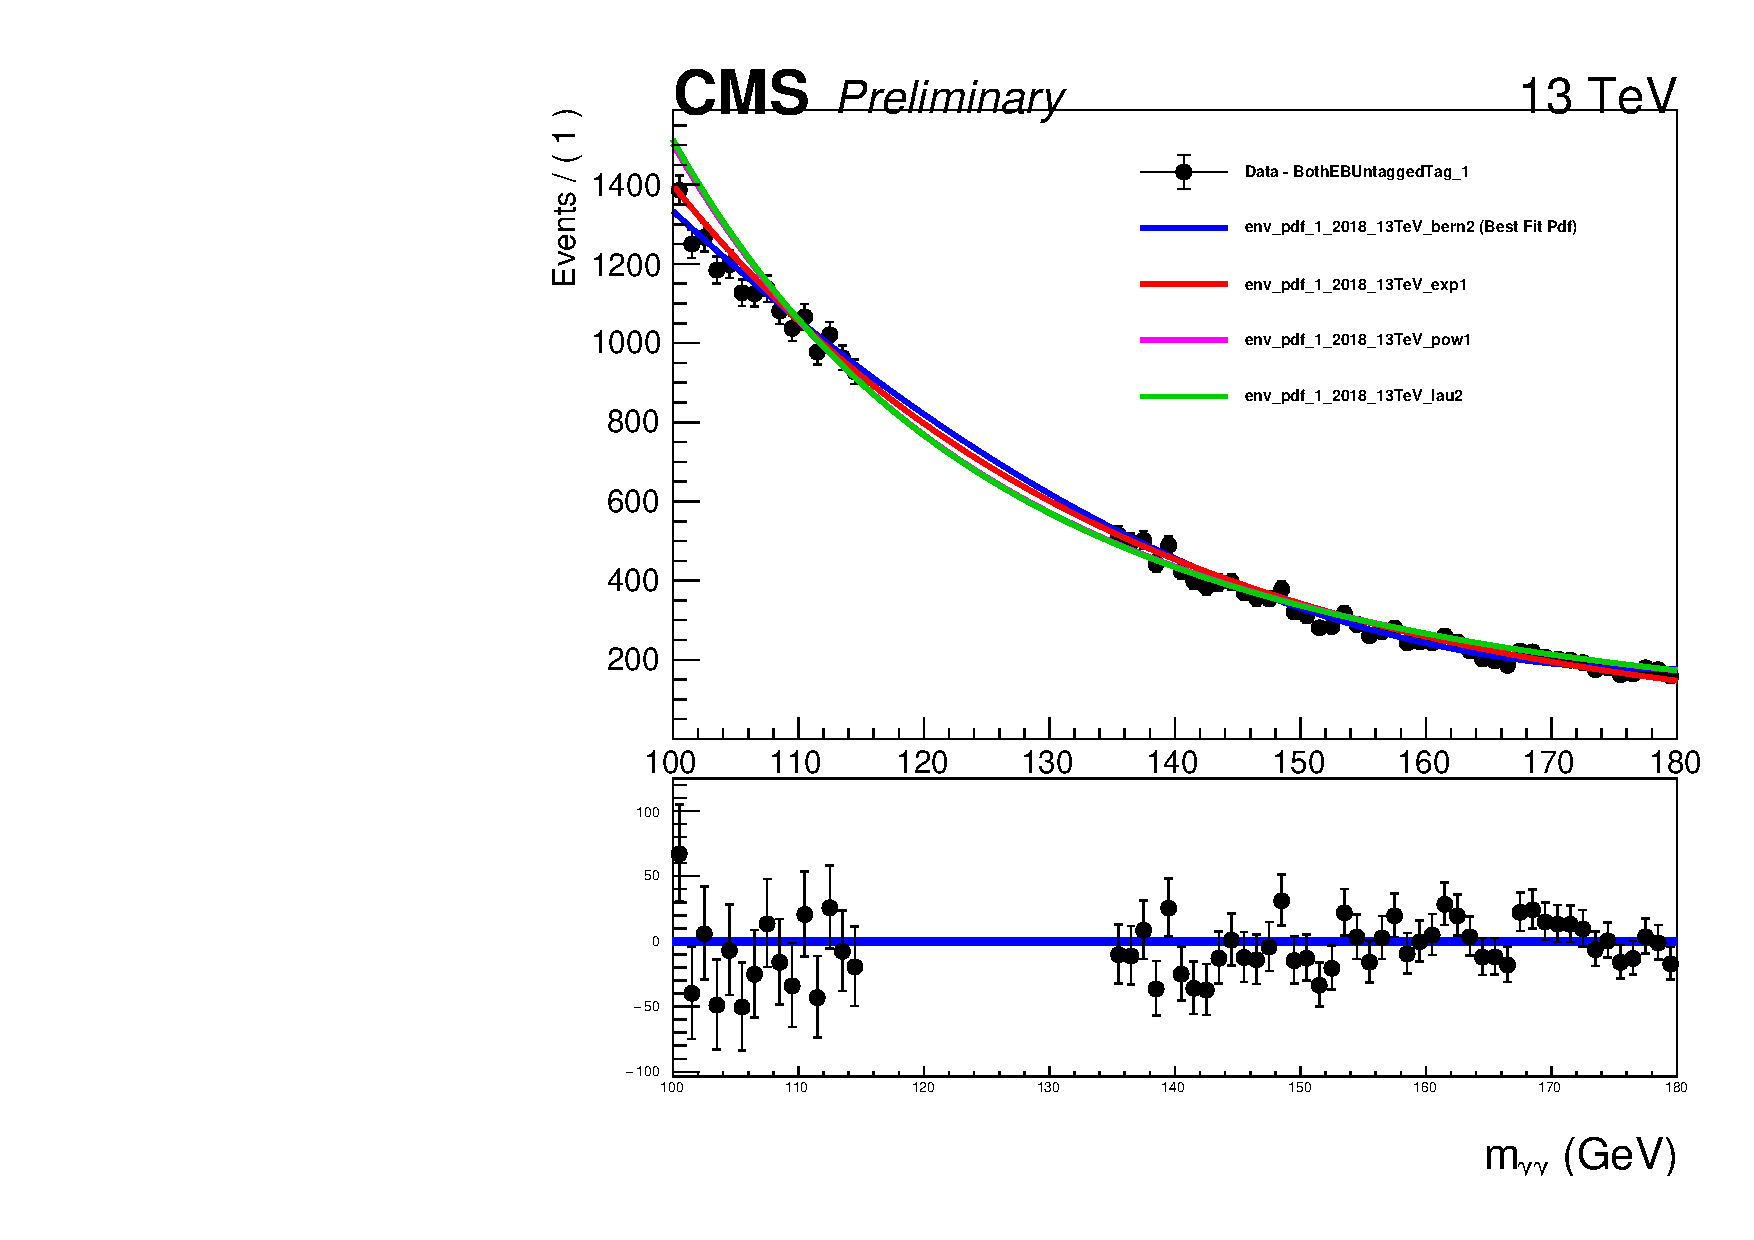
\includegraphics[width=0.925\textwidth]{07-figures/bkg_models/multipdf_BothEBUntaggedTag_1_2018.pdf}
            \end{center}
        \end{minipage}
    }~\subfloat{%
        \begin{minipage}[t]{0.5\textwidth}%
            \begin{center}
                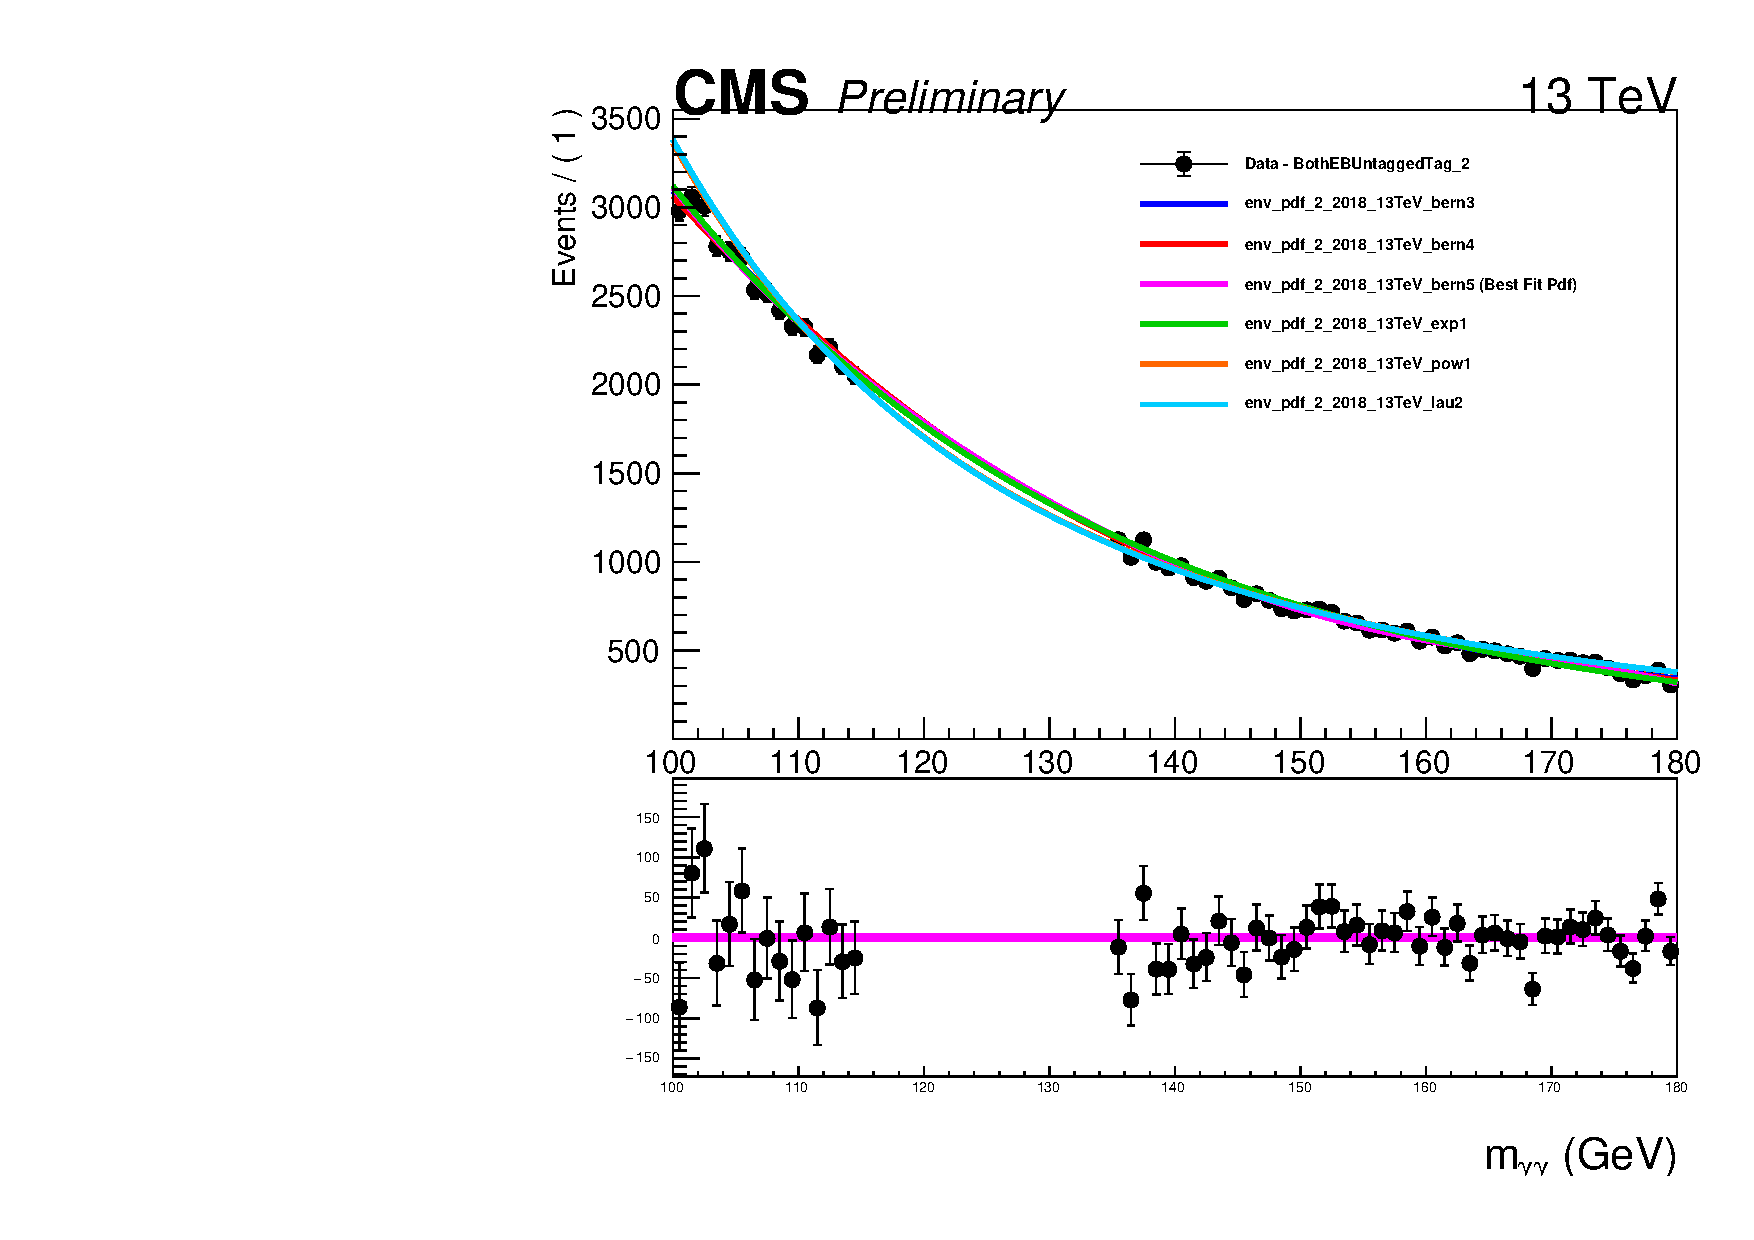
\includegraphics[width=0.925\textwidth]{07-figures/bkg_models/multipdf_BothEBUntaggedTag_2_2018.pdf}
            \end{center}
        \end{minipage}
    }~\subfloat{%
        \begin{minipage}[t]{0.5\textwidth}%
            \begin{center}
                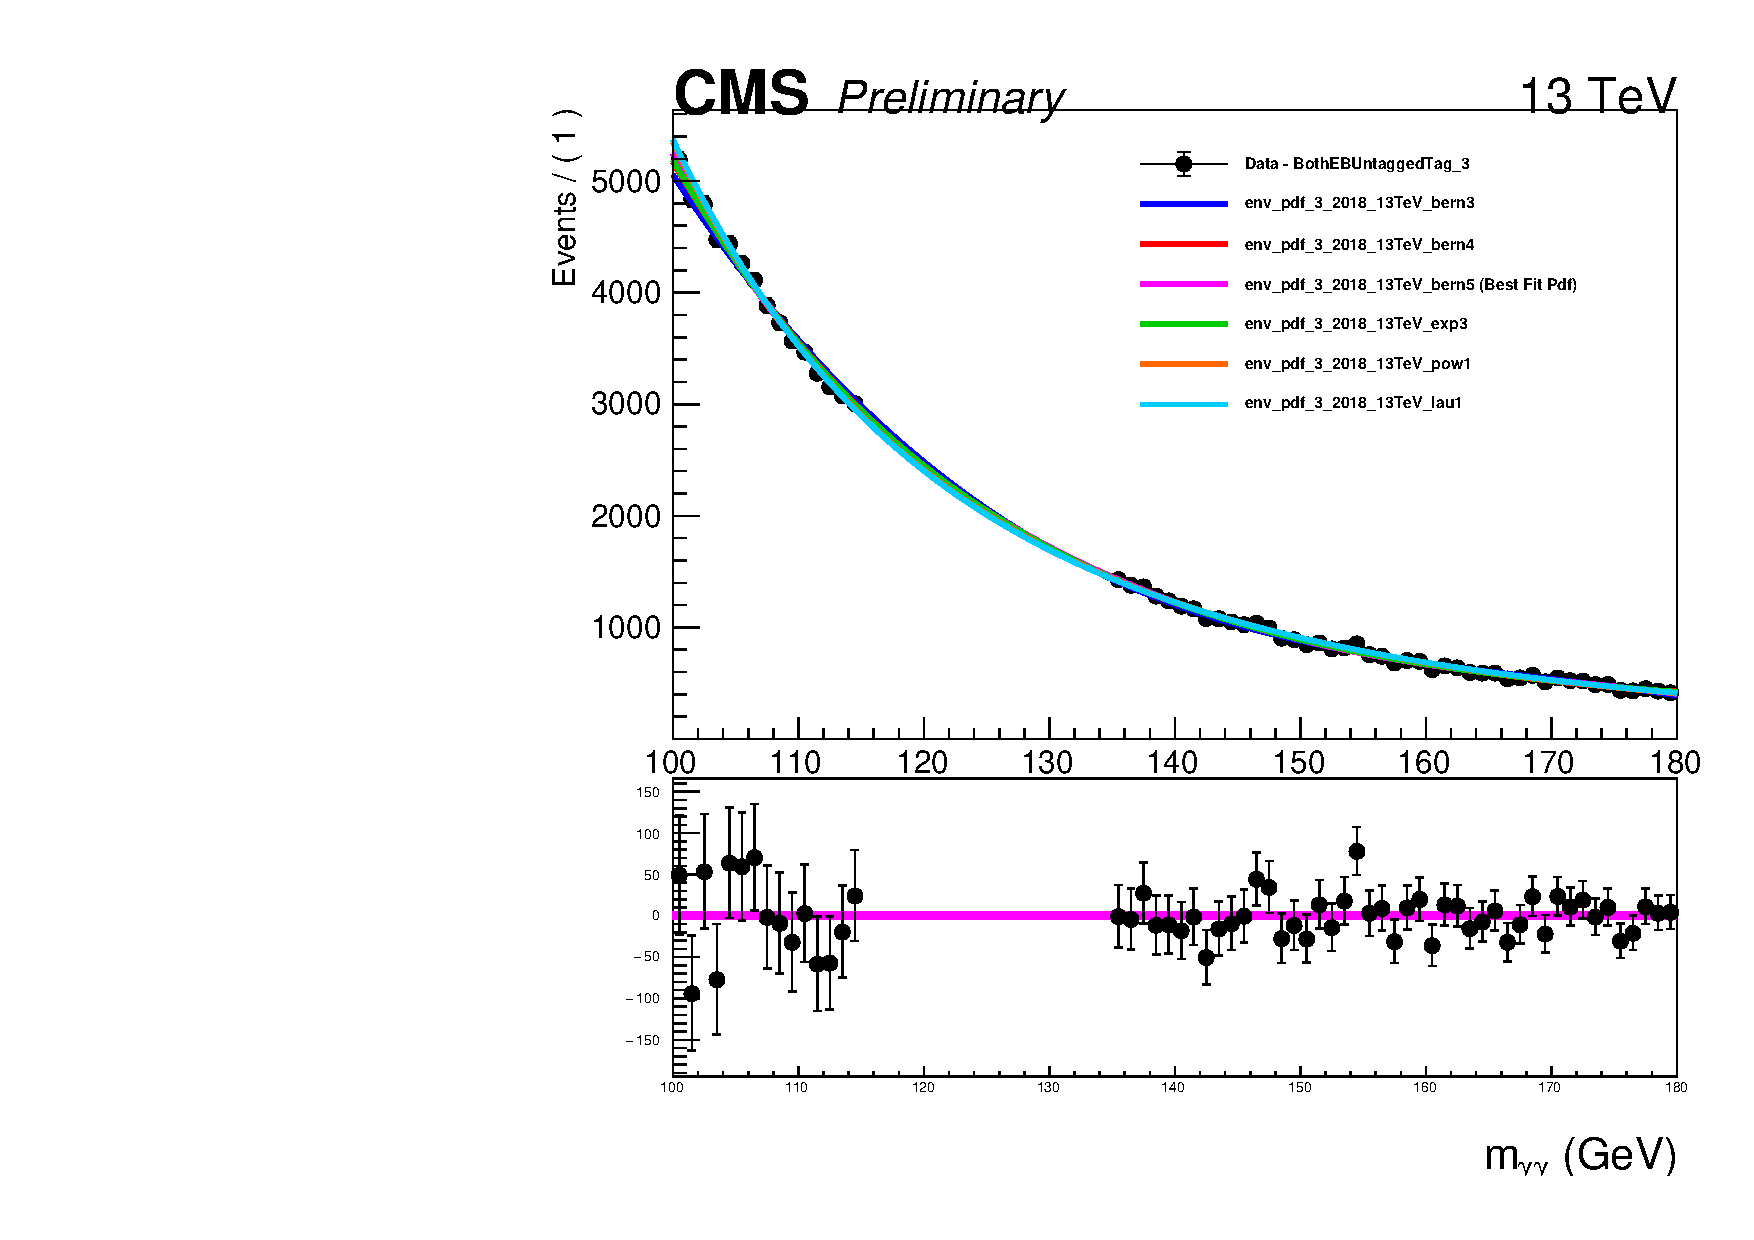
\includegraphics[width=0.925\textwidth]{07-figures/bkg_models/multipdf_BothEBUntaggedTag_3_2018.pdf}
            \end{center}
        \end{minipage}
    }
            \begin{center}
    \subfloat{%
        \begin{minipage}[t]{0.5\textwidth}%
                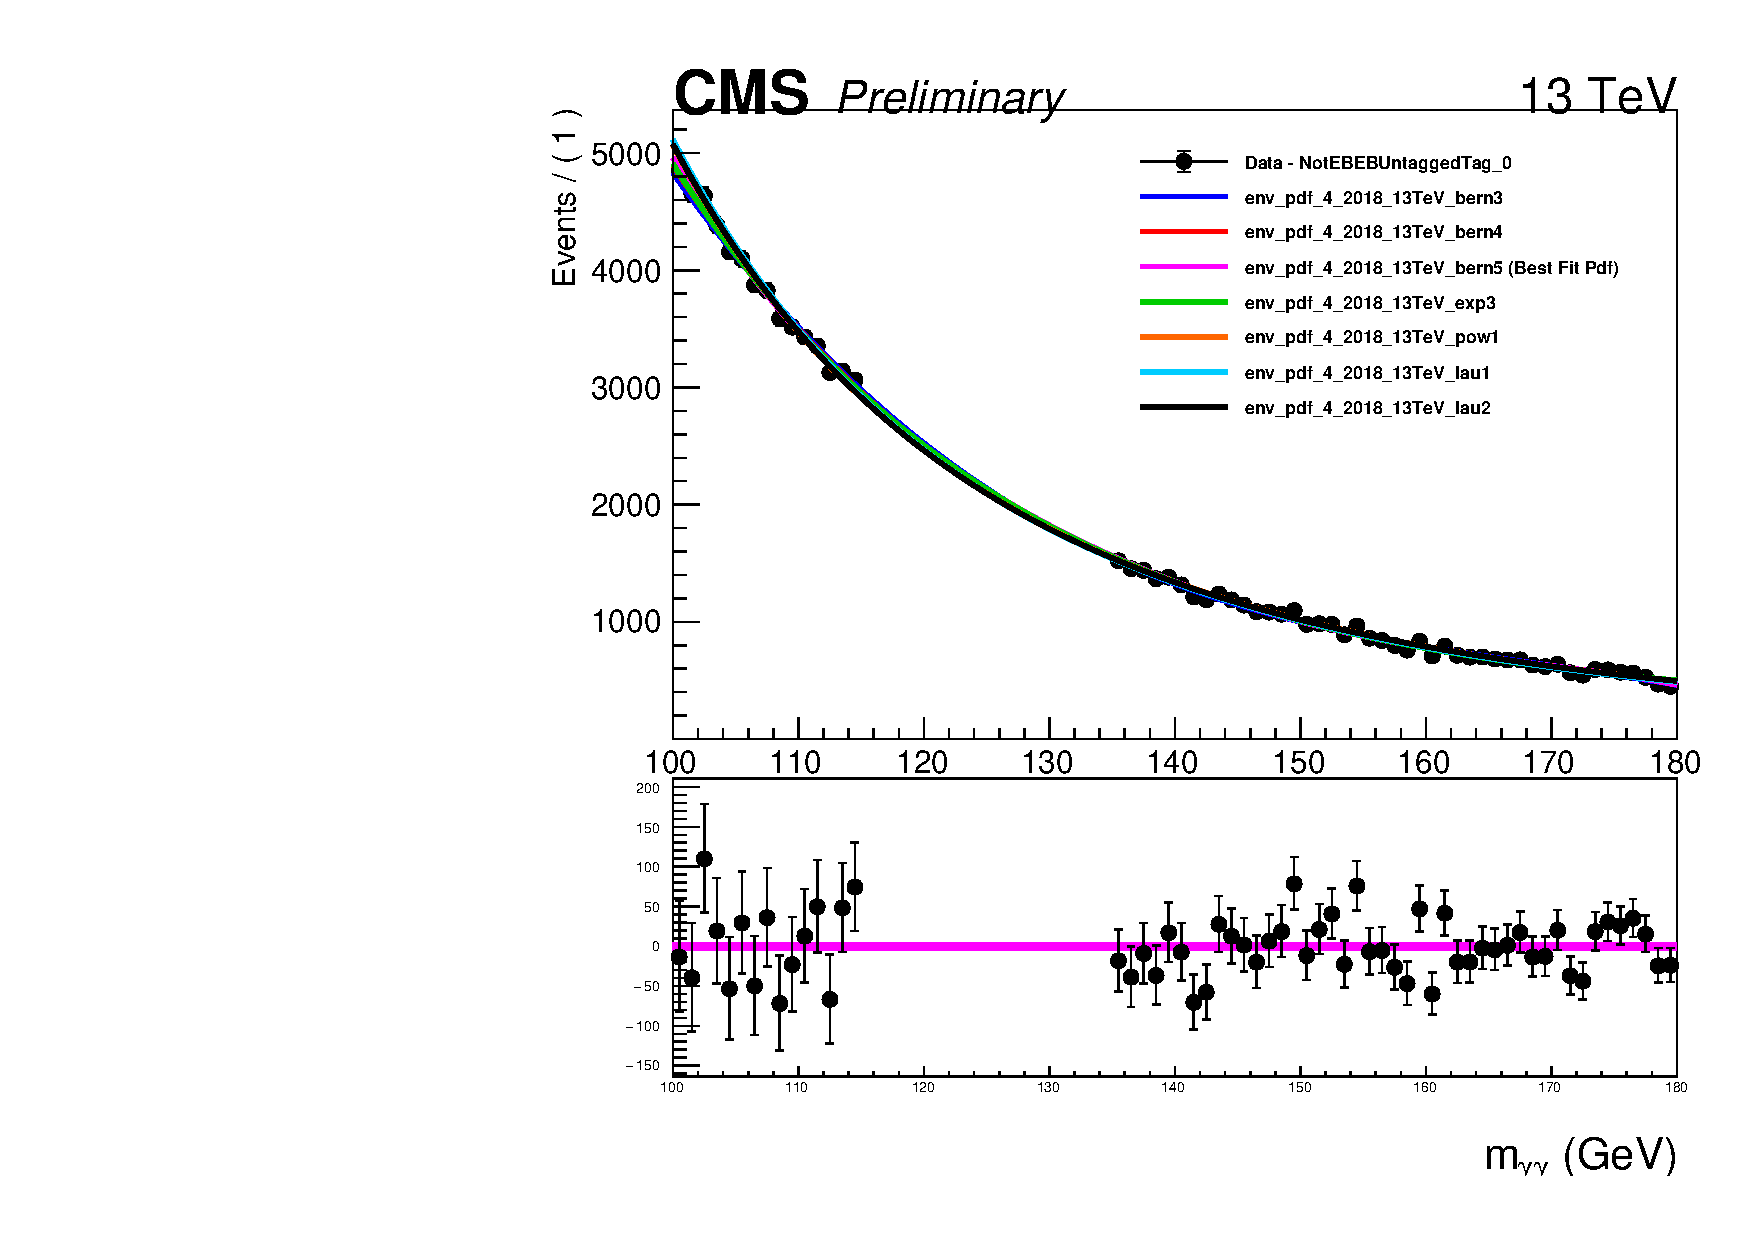
\includegraphics[width=0.925\textwidth]{07-figures/bkg_models/multipdf_NotEBEBUntaggedTag_0_2018.pdf}
        \end{minipage}
    }
            \end{center}
    \caption[Background models: 2018]{Background models for 2018 in each category.}
    \label{fig:bkg_model_2018}
\end{figure}

\begin{figure}[htbp!]
    \subfloat{%
        \begin{minipage}[t]{0.5\textwidth}%
            \begin{center}
                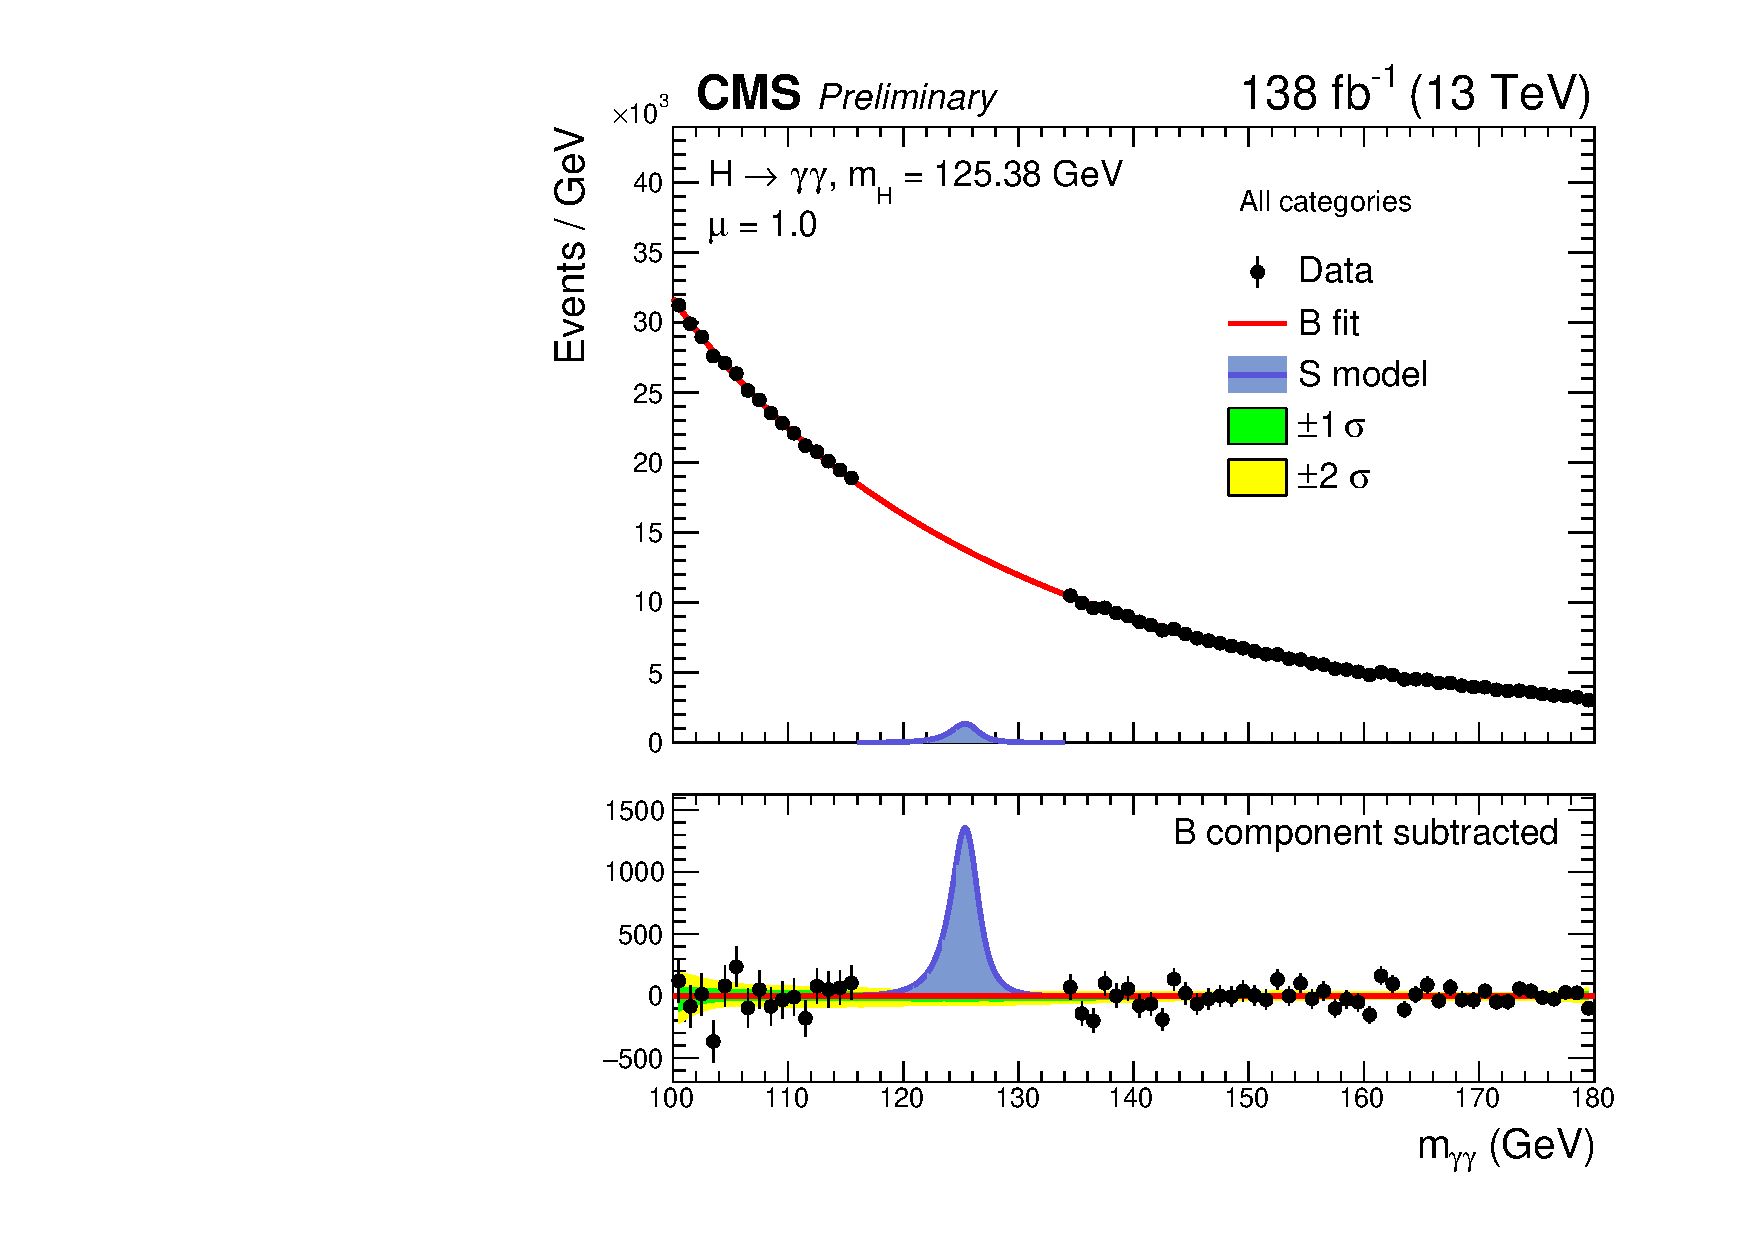
\includegraphics[width=\textwidth]{07-figures/all_CMS_hgg_mass.pdf}
            \end{center}
        \end{minipage}
    }~\subfloat{%
        \begin{minipage}[t]{0.5\textwidth}%
            \begin{center}
                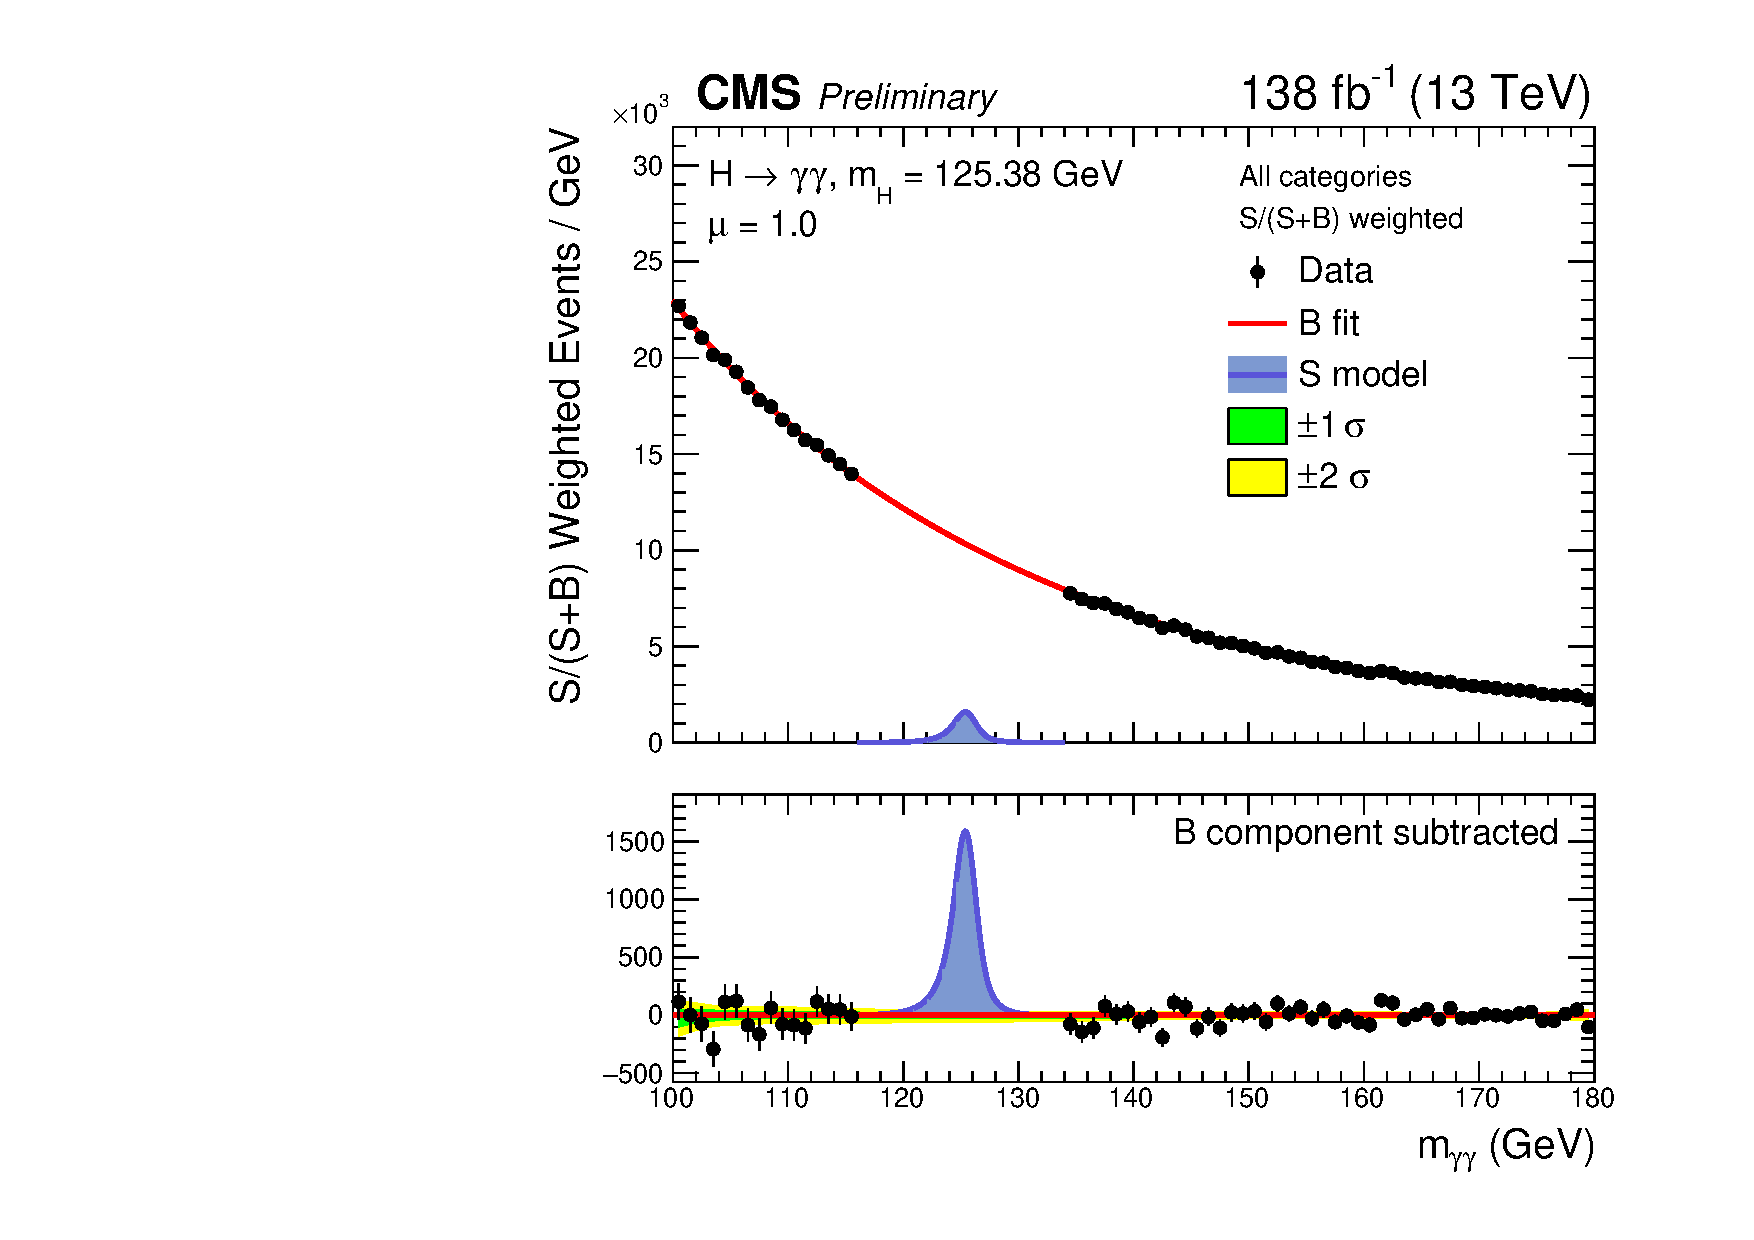
\includegraphics[width=\textwidth]{07-figures/wall_CMS_hgg_mass.pdf}
            \end{center}
        \end{minipage}
    }
            \begin{center}
    \subfloat{%
        \begin{minipage}[t]{0.55\textwidth}%
                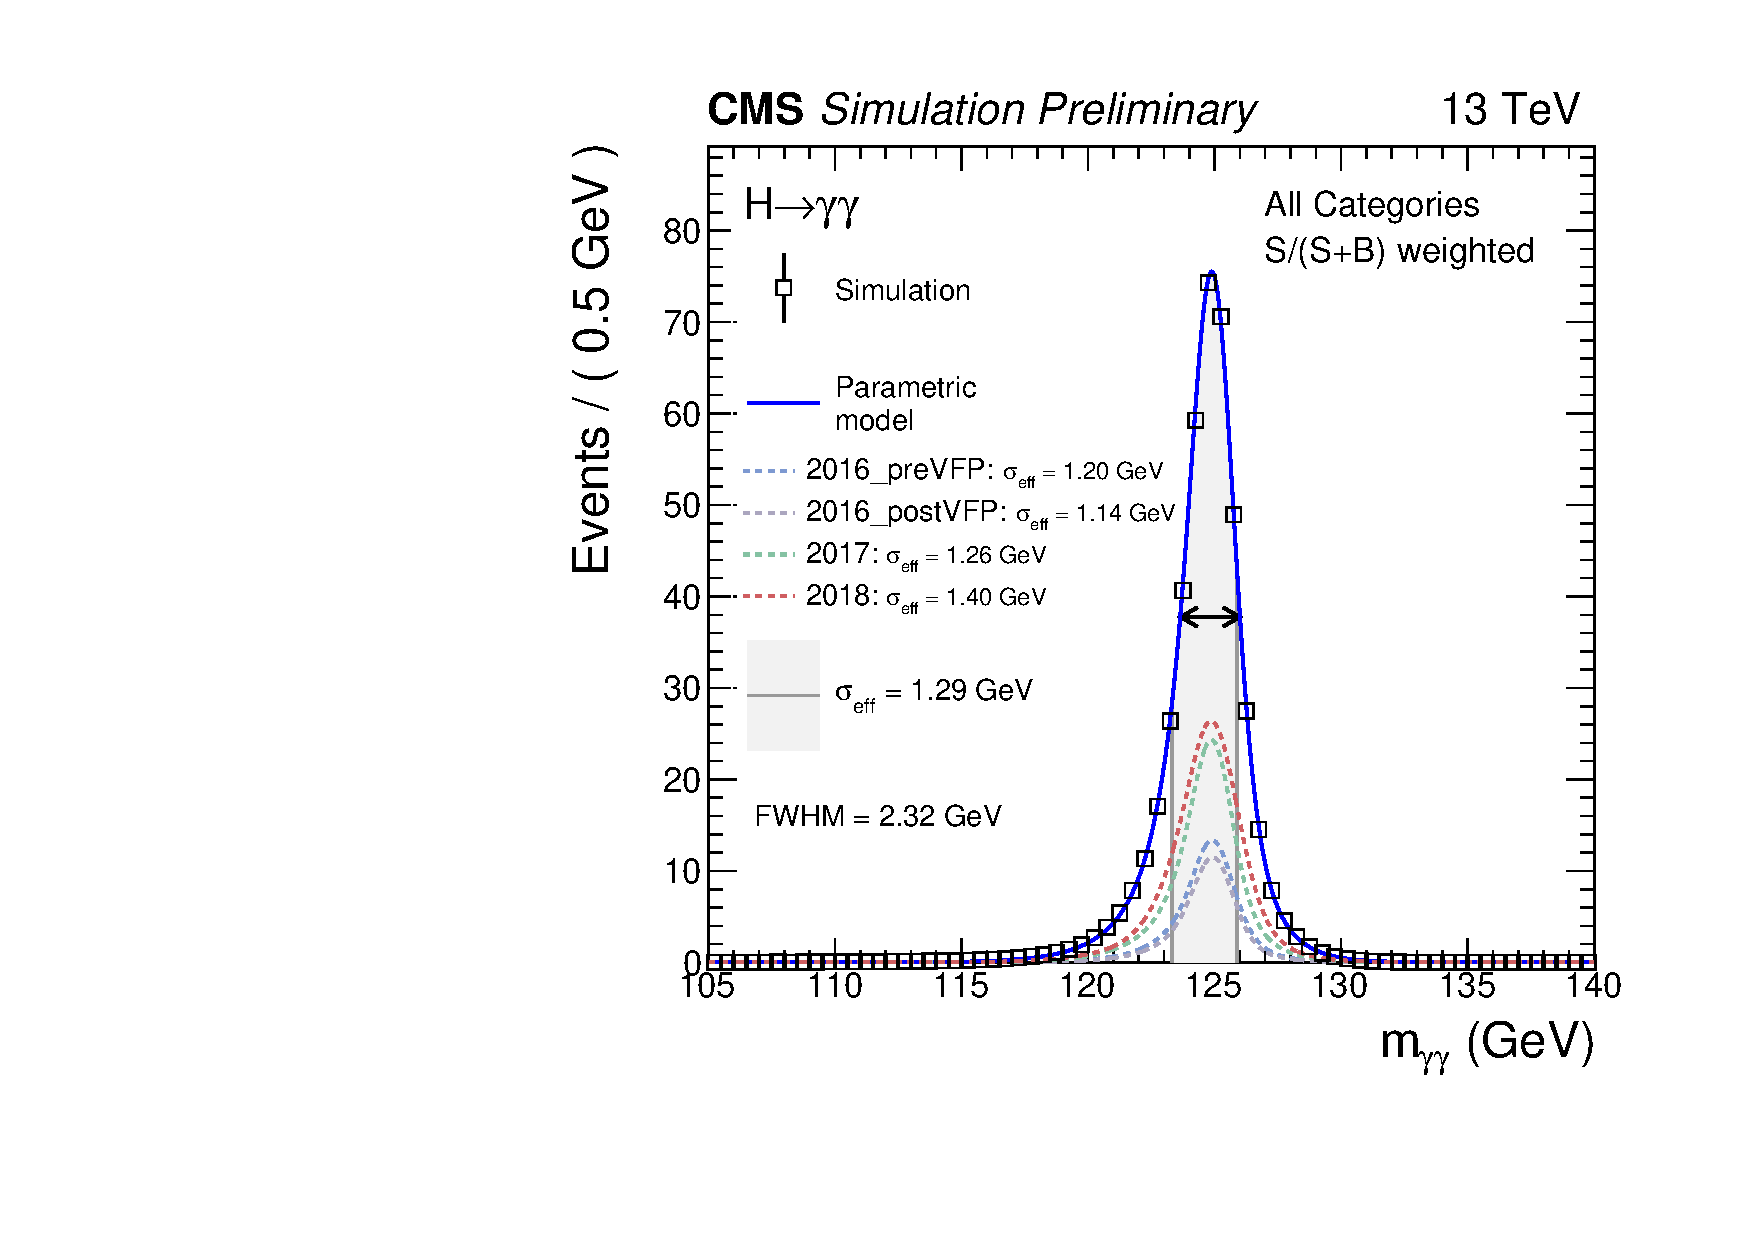
\includegraphics[width=\textwidth]{07-figures/smodel_wall.pdf}
        \end{minipage}
    }
            \end{center}
    \caption[Full Run 2 signal and background models]{Blinded signal + background model plots for the full Run 2 data-taking period. Both the unweighted sum of signal categories (upper left) and the S/(S+B)-weighted sum of signal categories (upper right) are shown. The best-fit background PDF choice (after an S+B fit to the data) is shown as a red line, along with the corresponding $\pm 1\sigma$ and $\pm 2\sigma$ uncertainty bands obtained from toy Asimov datasets. The signal modeling is also overlaid. A detailed description of the signal model is given as well (bottom).}
    \label{fig:model_run2}
\end{figure}





\begin{table}[]
\centering
\begin{tabular}{ccccc}
  \hline
  \hline
    category & $\sigma_{\textrm{eff}}$ & S & B & S/(S+B) \\
\hline
\multicolumn{5}{c}{UL2016\_preVFP} \\
\hline
BothEBUntaggedTag\_0 & 0.92 & 24.68 & 47.06 & 0.34 \\
BothEBUntaggedTag\_1 & 0.98 & 69.66 & 292.1 & 0.19 \\\
BothEBUntaggedTag\_2 & 1.18 & 98.33 & 751.31 & 0.12 \\
BothEBUntaggedTag\_3 & 1.46 & 163.51 & 2226.11 & 0.07 \\
NotEBEBUntaggedTag\_0 & 2.05 & 115.12 & 2679.16 & 0.04 \\
Total & 1.20 & 471.3 & 5995.74 & 0.07 \\
    \hline
\multicolumn{5}{c}{UL2016\_postVFP} \\
	\hline
BothEBUntaggedTag\_0 & 0.93 & 13.28 & 18.9 & 0.41 \\
BothEBUntaggedTag\_1 & 0.92 & 18.84 & 45.05 & 0.29 \\
BothEBUntaggedTag\_2 & 1.03 & 116.42 & 665.28 & 0.15 \\
BothEBUntaggedTag\_3 & 1.38 & 108.65 & 1271.94 & 0.08 \\
NotEBEBUntaggedTag\_0 & 1.99 & 98.69 & 2260.22 & 0.04 \\
Total & 1.14 & 355.88 & 4261.39 & 0.08 \\
    \hline
\multicolumn{5}{c}{UL2017} \\
\hline
BothEBUntaggedTag\_0 & 0.98 & 64.28 & 134.45 & 0.32 \\
BothEBUntaggedTag\_1 & 1.06 & 181.99 & 1002.72 & 0.15 \\
BothEBUntaggedTag\_2 & 1.29 & 242.21 & 2385.73 & 0.09 \\
BothEBUntaggedTag\_3 & 1.68 & 276.14 & 5283.5 & 0.05 \\
NotEBEBUntaggedTag\_0 & 2.25 & 225.16 & 5718.85 & 0.04 \\
Total & 1.26 & 989.78 & 14525.25 & 0.06 \\
    \hline
\multicolumn{5}{c}{UL2018} \\
	\hline
BothEBUntaggedTag\_0 & 1.14 & 81.45 & 214.22 & 0.28 \\
BothEBUntaggedTag\_1 & 1.19 & 263.45 & 1702.17 & 0.13 \\
BothEBUntaggedTag\_2 & 1.43 & 389.89 & 4435.63 & 0.08 \\
BothEBUntaggedTag\_3 & 1.78 & 343.68 & 7293.33 & 0.05 \\
NotEBEBUntaggedTag\_0 & 2.24 & 345.52 & 9572.98 & 0.03 \\
Total & 1.40 & 1423.99 & 23218.33 & 0.06 \\
\hline
\hline
\end{tabular}
\caption[Signal and background yields]{Signal and background yields for each category and year, along with values for $\sigma_{\textrm{eff}}$ and S/(S+B).}
\label{tab:yields}
\end{table}
